\documentclass[openany]{book}
\usepackage[utf8]{inputenc}
\usepackage{fullpage}
\usepackage{float}
\usepackage{graphics}
\usepackage{graphicx}
\usepackage{csquotes}
\usepackage{hyperref}
\usepackage{amsmath}
\usepackage{tikz}
\usepackage{pgfplots}
\usepackage{tikz-3dplot}
\usepackage{import}
\usepackage{color}
\usepackage{amssymb}
\usepackage{epstopdf}
\usepackage{bold-extra}
\usepackage{caption}
\usepackage{subcaption}	
\usepackage[T1]{fontenc}
\usepackage{xargs}
\usepackage{etoolbox}
\usepackage{multirow}

\bibliographystyle{unsrt} 

\setlength\parindent{0pt}
\raggedbottom
\begin{document}

		\begin{titlepage}
		\centering
		
		{\Huge Astrophysical S-factor calculation for selected reactions  \par}
		
		\begin{figure}[H]
			\centering
			
\includegraphics[width=0.5\linewidth]{logo.pdf}
			\label{fig:logo}
		\end{figure}
		{\Large Author:  \par}
		{\Large Carlos Alberto Calvachi Salas \par}
		{\Large 201822667 \par}
		\vfill
		{\Large\textit{Final project submitted in partial fulfillment of the requirements for the degree of} \par}
		\vfill
		{\Large\textit{Physicist} \par}
		\vfill
		{\Large Advisor:  \par}
		{\Large Neelima Govind Kelkar Ph.D. \par}
		\vfill
		{\Large Universidad de los Andes  \par}
		{\Large Physics Department  \par}
		{\Large January, 2023  \par}
		{\Large Bogotá, Colombia \par}
	\end{titlepage}


\chapter*{Acknowledgments}

To my Mom for everything you have done in our lives with infinite strength, courage and love. \\

To my family for their existence and memory. A deep special thanks for my aunt Mary for her unique continuous support and grandmother Marianita for her peculiar intensity in caring about us. \\

To professor Neelima for her essential guidance, expertise and encouragement during the development and preparation of this project.  \\ 

To my professors and fellow students for the diverse moments lived and the lessons learned. \\

To my university for partially financing my education with the special career credit.  \\

\chapter*{Abstract}

Despite the vast success of nuclear astrophysics in predicting the relative composition of the lightest elements in the early Universe, current theoretical and experimental knowledge of reactions at astrophysical low energies requires severe improvement. This work is centered in calculating the S-factor, which is a relevant quantity for low energy extrapolation. Initially, a literature survey is performed to present a diverse selection of models, which include empirical, potential, microscopical and R-matrix approaches. These models useful for S-factor computation at recurrent astrophysical environments, which generally comprehend Big Bang, stellar, explosive and exotic nucleosynthesis. Then, S-factor experimental data of relevant reactions is selected to be contrasted with predictions of potential and empirical models. Additionally, the effects of resonances and electron screening are analyzed for improving and consolidating the S-factor estimation. \\

A pesar del gran éxito de la astrofísica nuclear en la predicción de la composición relativa de los elementos más ligeros en el Universo temprano, el conocimiento teórico y experimental de las reacciones a energías astrofísicas bajas requiere una mejora sustancial. Este trabajo se centra en el cálculo del factor S, que es una cantidad relevante para la extrapolación a bajas energías. Inicialmente, una revisión de literatura es realizada con el fin de presentar una diversa selección de modelos, que incluye las aproximaciones empíricas, potencial, microscópica y de matriz R. Estos modelos son útiles para el cómputo del factor S en ambientes astrofísicos usuales, los cuales comprenden en general nucleosíntesis en ambientes como el Big Bang, las estrellas y de tipo exótico y explosivo. En seguida, los datos experimentales del factor S son contrastados con predicciones de modelos potenciales y empíricos. Adicionalmente, los efectos de las resonancias, así como del apuntalamiento electrónico, son analizados para mejorar y consolidar la estimación del factor S. \\

%Keywords 
%	Nuclear astrophysics
%	Astrophysical S-factor
%	Literature survey
%	Nuclear reactions
%	Resonant phenomena
%	Screening effect 
%	Astrophysical environments
%	Experimental data fitting 
	
	
\clearpage

\tableofcontents
\listoffigures
\listoftables

\newcommand{\reaction}[8]{
	
	\mathrm{{}^{#1}#2({}^{#3}#4, {}^{#5}#6){}^{#7}#8 }

}

\newcommand{\graph}[3]{
	
\begin{figure}[H]
	\centering
	\includegraphics{Graphs/#1.eps}
	\caption[#2]{#3}
	\label{fig:#1}
\end{figure}

}


\newcommand{\radiativeCapture}[1][p]{
	(#1, \gamma)
}

\newcommandx*{\Cfusion}[2][1=12, 2=12]{
	\mathrm{{}^{#1}C +  {}^{#2}C}
}

\newcommandx*{\Ofusion}[2][1=16, 2=16]{
	\mathrm{{}^{#1}O +  {}^{#2}O}
}

\newcommand{\ddexchange}{\mathrm{{}^{2}H(d, p){}^{3}H}}
\newcommand{\dRadiativeCapture}{\mathrm{{}^{2}H(p, \gamma){}^{3}He}}
\newcommand{\BeRadiativeCapture}{\mathrm{{}^{7}Be(p, \gamma){}^{8}B}}
\newcommand{\CRadiativeCapture}{\mathrm{{}^{13}C(p, \gamma){}^{14}N}}

\newcommandx*{\subGraph}[3][3 = 0]{
	\ifnumodd{#3}
	{\begin{subfigure}[b]{0.90\linewidth}
			\centering 
			\includegraphics[width=\linewidth]{Graphs/#1}
			\caption{#2\label{sfig:#1}}
	\end{subfigure}}
	{\begin{subfigure}[b]{0.48\linewidth}
			\centering 
			\includegraphics[width=\linewidth]{Graphs/#1}
			\caption{#2\label{sfig:#1}}
	\end{subfigure}}
}


\newcommand{\graphWrapper}[4]{
	\begin{figure}[H]
		\centering
		#1
		\caption[#3]{#4}
		\label{fig:#2}
	\end{figure}
}

\newcommand{\multiGraphs}[4]{
	\newcounter{n}
	\newcounter{m}
	\newcounter{l}
	\newcounter{a}
	\newcounter{b}

	\setcounter{n}{0}
	\setcounter{m}{0}
	\setcounter{l}{0}
	\setcounter{a}{0}
	\setcounter{b}{0}
	
	
	\def \textSubFigCaption {}
	
	
	\foreach \x in #1{
		\stepcounter{m}
	}
	
	
	
	\begin{figure}[H]
		\centering
		\foreach \x in #1{
			\stepcounter{n}
			%\foreach \y in \x {\stepcounter{a}\ifnumodd{\thea}{\y}{}}
			%\foreach \y in \x {\stepcounter{b}\ifnumodd{\theb}{}{\y}}
			%\ifthenelse{\then = \them \AND \isodd{\them}}{1}{0}
						\ifthenelse{\then = \them \AND \isodd{\them} }{\begin{subfigure}[b]{0.90\linewidth}}{\begin{subfigure}[b]{0.45\linewidth}}
					\centering
					\foreach \y in \x {
						\stepcounter{l}
						\ifnumodd{\thel}{\includegraphics[width=\linewidth]{Graphs/\y.eps}}
						{\caption{\y}}
					}
				\end{subfigure}
				\setcounter{l}{0}
				\foreach \y in \x {
					\stepcounter{l}
					\ifnumodd{\thel}{\label{sfig:\y}}{}
				}
			%\subGraph{16O18O}{$\Ofusion[16][18]$ reaction.}
			
		}
		\caption[#3]{#4}
		\label{fig:#2}
	\end{figure}
}


\chapter*{Introduction}

Astrophysics and nuclear physics are intimately connected by nucleosynthesis. The vast diversity of elements in the Universe is frequently explained by the study of subtleties involving nuclear reactions. Then, extensive attention has been provided to predict and measure the behavior of critical nuclear reactions. However, many current experiments are unable to reach the energy of stellar fusion, which is a considerable upset when predicting the distributions of most elements. This setback motivates why theoretical modeling is essential to extrapolate knowledge from the high energy achievable by earth experiments to low energy behavior relevant at stellar environments. The aim of this work is to calculate a relevant extrapolation quantity, the astrophysical S-factor, in a selection of few resonant and non-resonant nuclear reactions of interest. A diagram which illustrates the dependence among chapters is given in Figure \ref{fig:DependenceChart}. \\

In Chapter \ref{ch:nuclearAstrophysics}, nuclear astrophysics general fundamentals are presented. Initially, some elementary aspects about the nucleus, its composition and models are introduced. Then, selected topics on quantum mechanics including scattering, tunneling, perturbation and angular momentum theory are mentioned. Next, basic concepts on nuclear reactions are introduced. Finally, the astrophysical S-factor is defined and exemplified. \\

Later, in Chapter \ref{ch:reactionsInterest}, reactions of interest are introduced by classifying them with the astrophysical environment they are more relevant to. The selection includes reactions from Big Bang nucleosynthesis (BNN), stellar fusion, more particularly hydrogen burning (pp-chain), carbon, nitrogen and oxygen cycles (CNO and HCNO), and middle heavy fusion environments, involving heavy nuclei burning, with the alpha, neutron (s and r) and proton (p and rp) capture processes. Lastly, some active research topics are surveyed. \\

Then, astrophysical models for S-factor calculations are introduced in Chapter \ref{ch:sfactorModels}. This part begins by covering more sophisticated models, like microscopic, which are based on quantum-mechanical calculations including nuclear substructures, and matrix models, particularly the R-matrix formalism. Later, more phenomenological approaches are encountered including the potential models, which assume the existence of an effective interaction between nuclei and empirical formulas later. A distinctive feature of the latter is that it permits S-factor calculation directly with an energy dependent formula. Meanwhile, the vast majority of the former three models require the computation of the cross section of the reaction. \\

Finally, S-factor calculations are presented in Chapter \ref{ch:sfactorCalculations}. The purpose of this part is to compute the astrophysical S-factor for the non-resonant behavior of the light $\ddexchange$, $\dRadiativeCapture$ and middle $\Cfusion$, $\Ofusion$, $\Ofusion[16][17]$, $\Ofusion[16][18]$ and $\mathrm{{}^{12}C + {}^{16}O}$ heavy reactions. Additionally, it is evaluated how the non-resonant background is complemented with a Brieit-Wigner like resonant contribution for the selected $\CRadiativeCapture$ and $\BeRadiativeCapture$ reactions. In all the calculations, empirical formula fitting is performed to obtain the best estimations. In particular, in the case of the $\ddexchange$ reaction, S-factor calculations improve by introducing an additional enhancement factor, which accounts for the electron screening effect, to the background estimation formula.
 
\begin{figure}[H]
	\centering 
	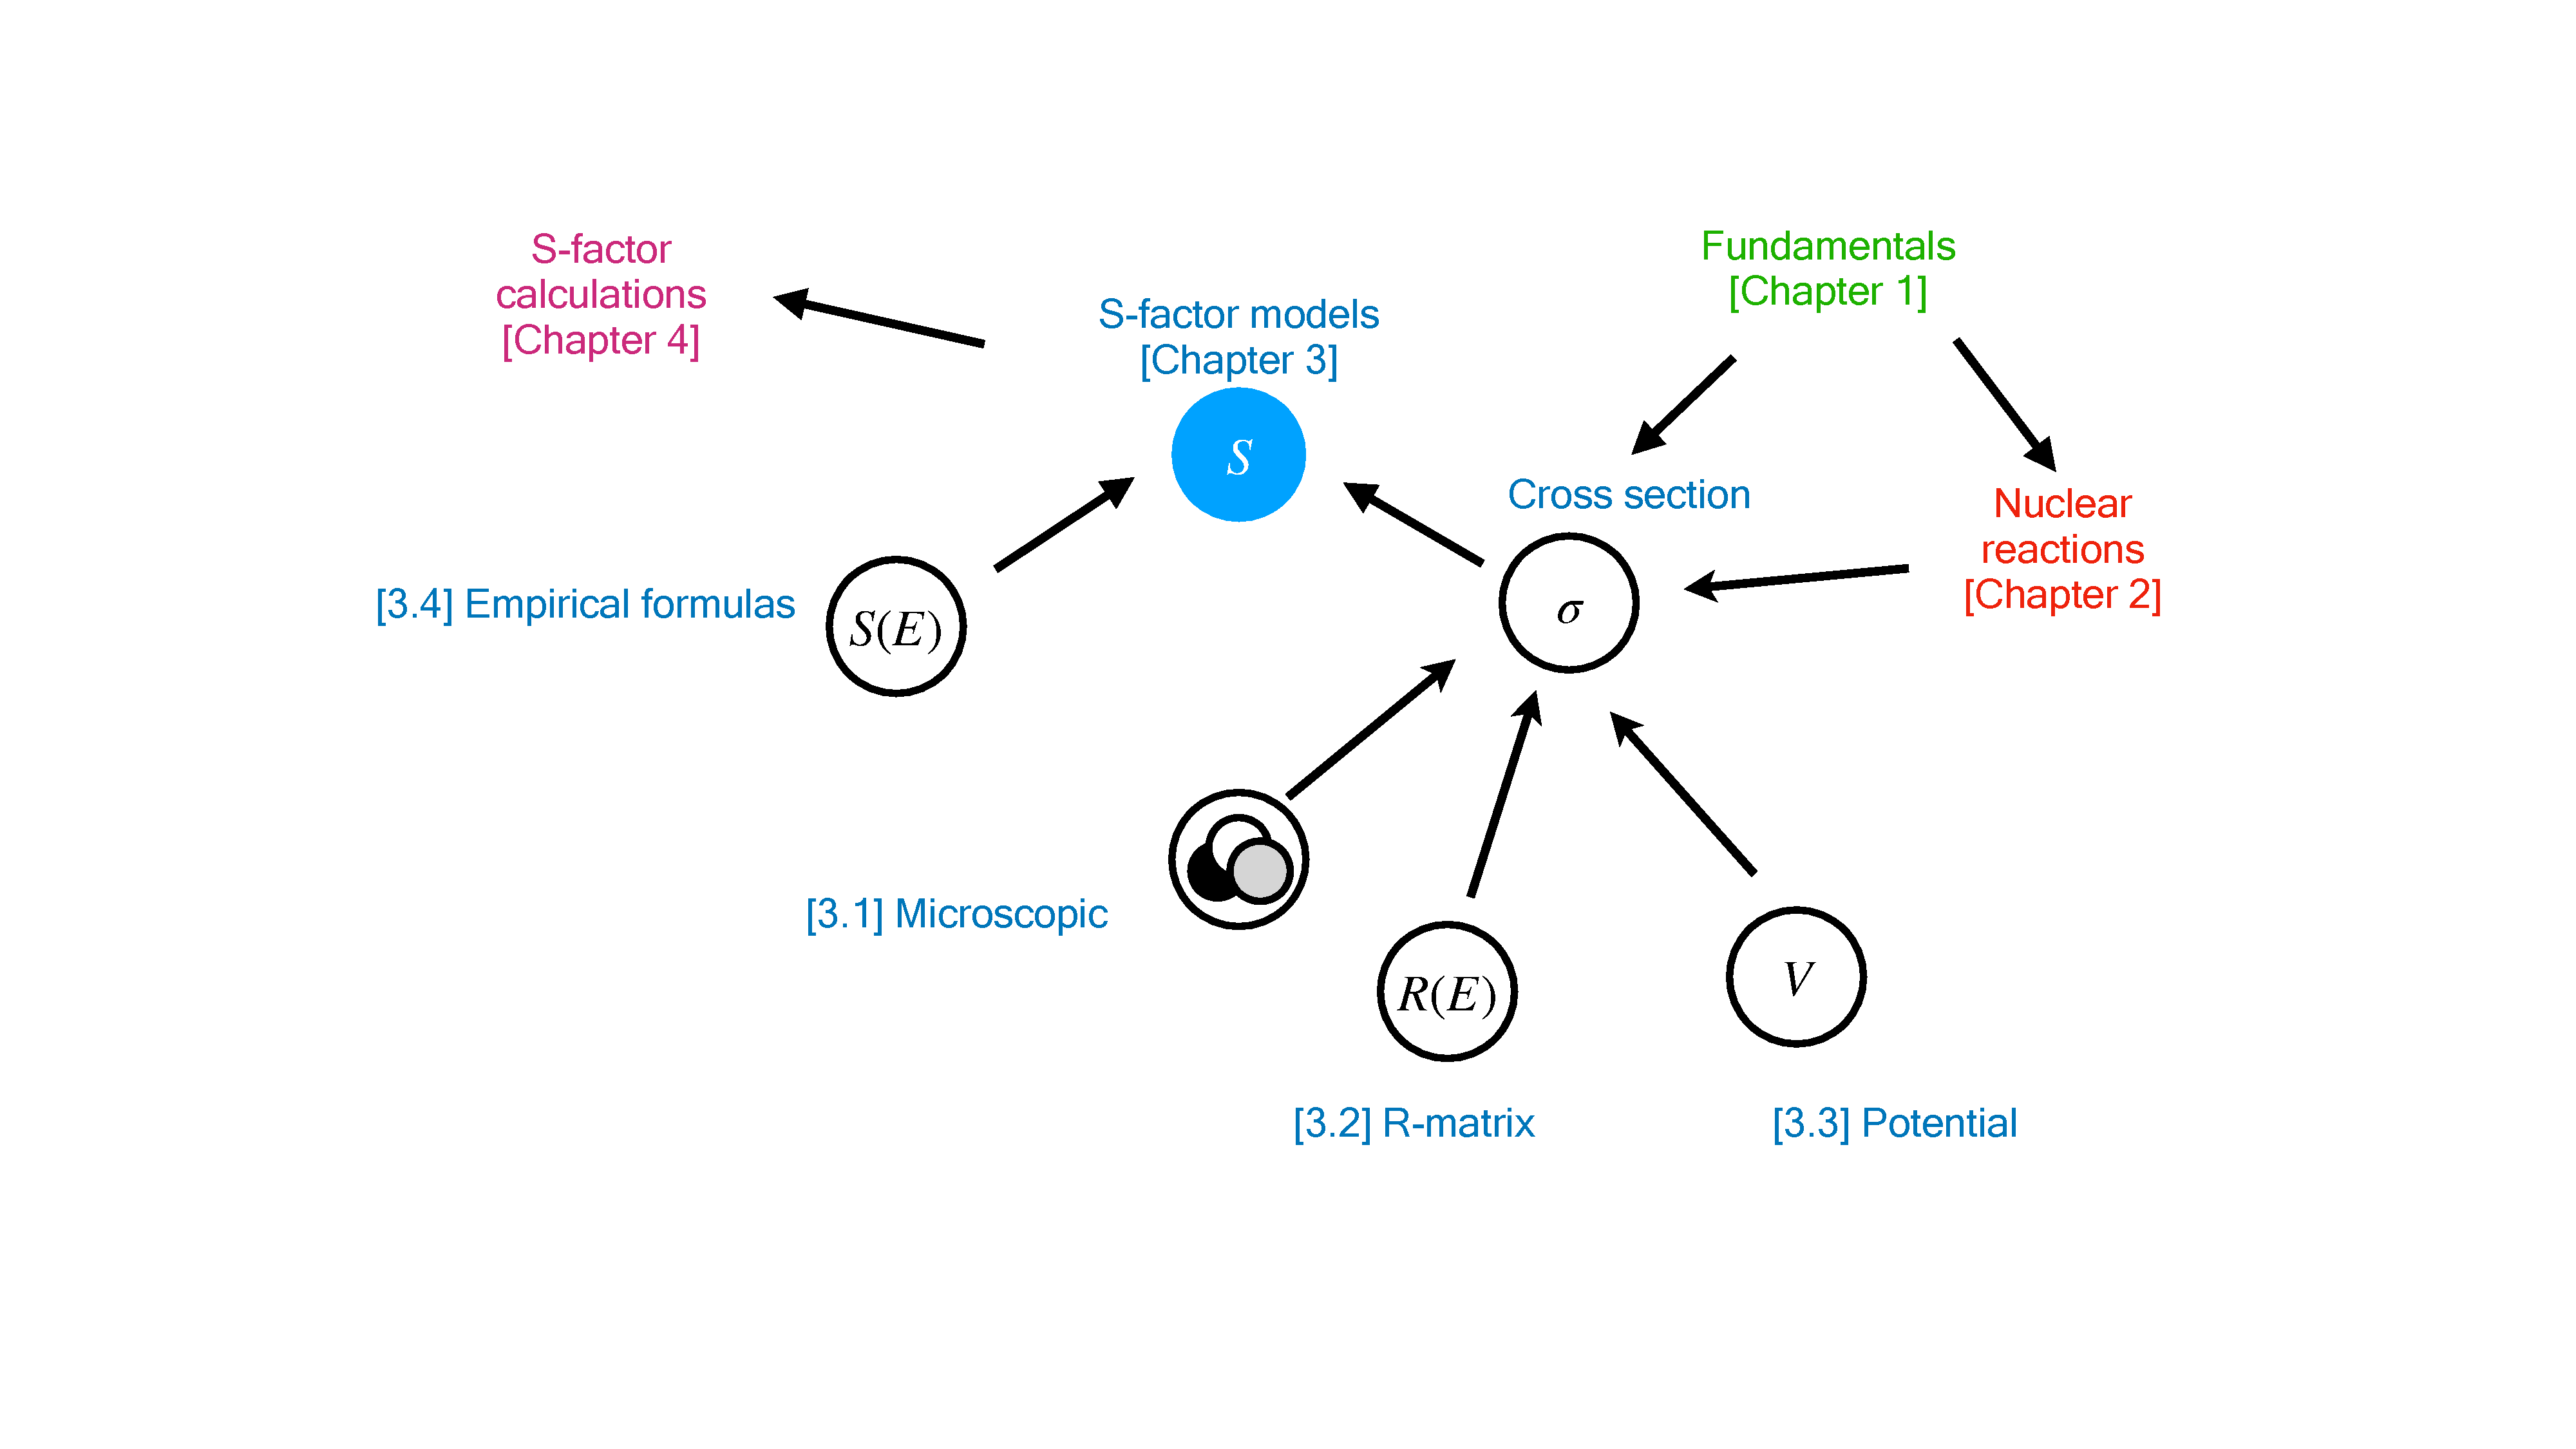
\includegraphics[scale=0.28]{Graphs/DependenceChart}
	\caption[Dependence chart.]{Dependence chart between chapters and S-factor model sections of Chapter \ref{ch:sfactorModels}.}
	\label{fig:DependenceChart}
\end{figure}

\chapter{Nuclear astrophysics fundamentals}  \label{ch:nuclearAstrophysics}

In order to apply nuclear astrophysics to the study of element production, there are essentials to be considered. The aim of this Chapter is to provide a general review of the main points relevant for nuclear astrophysics. Initially, some introductory aspects of the nucleus are reviewed. Then, selected quantum mechanics topics pivotal for nuclear phenomena understanding are surveyed. Later, aspects on nuclear structure and reactions are included. Lastly, the astrophysical S-factor is defined and exemplified. \\

The content included in this introductory Chapter was in part inspired from material offered by various textbooks. Some aspects of the nucleus were contributed by the Basdevant et al. textbook \cite{basdevant_rich_spiro_2004}. In the case of concepts, particularly nuclear structure, the material presented in the Heyde \cite{heyde_2004} and Bohr \& Mottelson \cite{bohr_mottelson_1998} books turn out to be useful. For scattering theory, tunneling phenomena topics the Illiadis \cite{iliadis_2015}, Joachain \cite{joachain_1975} and Newton \cite{newton_2002} textbooks were preferred respectively. Additionally, the book \cite{dick_2016} served as a source for perturbation theory and angular momentum discussions.

\section{General aspects about the nucleus} \label{sec:nucleiAspects}

The nucleus is a bound state of a system of nucleons with two types: protons and neutrons. While the former are positively charged and stable, the latter are uncharged and unstable.  They also have several quantum numbers associated to like angular momentum, spin, isospin and parity. Additionally, nucleons obey the Pauli-exclusion principle. Then, it is not possible to find them in the same single state. \\

Nuclear stability is explained by considering the effects of the repulsive long range Coulomb interaction and the attractive short range strong nuclear force. Particularly, protons and neutrons are bonded in the nuclei by the strong force which compensates electromagnetic repulsion. The classical way for quantifying nuclear stability is by computing the binding energy defined as: 

\begin{equation} \label{eq:restEnergy}
	B(A, Z) = Zm_pc^2 + (A-Z)m_nc^2 - E_0,
\end{equation}

where $Z$, $A$ are the atomic and mass number respectively and $m_p$ with $m_n$ is the pair of proton and neutron masses. In addition, $E_0 = Mc^2$ with $M$ being the mass of the nuclei. It is essential to be noticed that the mass of the nucleus usually is not equal to the sum of the masses of its nucleons. Namely, $M \neq Zm_p + (N - Z)m_n$. Then, it is possible to relate $B(A, Z)$ to a nuclear separation energy such that more stable nuclei have higher binding energy values. The shape of latter is pictured by considering most of the known nuclei in the graph of Figure \ref{fig:BindingEnergyCurve}.

\graph{BindingEnergyCurve}{Binding energy per nucleon curve}{Binding energy per nucleon $B/A$ characteristic curve. Each scatter-point represents a nucleus. The plot has an overall ascending behavior until it reaches the stability peak, which is located roughly below 9MeV. Then, at higher mass numbers, the behavior consists of a less sharper descent. $B/A$ values were calculated from data given by the JENDL database \cite{iwamoto_iwamoto_shibata_ichihara_kunieda_minato_nakayama_2020}.}

Each nucleus is characterized by the pair of numbers of protons and nucleons $(Z, A)$, and by a quantum state, which is usually comes with a unique set of quantum numbers like spin, angular momentum, parity. Additionally, a nucleus can be in the ground state, which is associated with the minimum energy state, or in an excited state, with a higher energy level. Nuclear identity is changed by different quantum mechanical ruled processes.  Strong, weak and electromagnetic interactions participate in determining the kinds of transformations that a nucleus have. 	All the processes have conservation laws related to the kind of interaction present. They impose restrictions to the nature of the interacting bodies, as well as to the values of the quantum numbers of their states. For example, while angular momentum is conserved in all reactions, parity or isospin conservation might be violated for specific weak force mediated processes.  \\

Decays are the first kind of classical nuclear identity changing processes. The general picture of this reaction is given by: 

\begin{equation} \label{eq:decay_general}
	X \rightarrow X' + A,
\end{equation}

where $X$ and $X'$ represent the decaying and surging nuclei respectively. Moreover, $A$ condenses all the decaying products. Usually this process privileges $X'$ to be more stable than $X$, which is the case of radioactive decay. Depending on the identity of $A$, decays can be classified. Processes are referred to alpha, beta and gamma when $A$ is a helium $\mathrm{{}^{4}He}$ nucleus, a pair of electrons and antineutrino $e^{-} + \bar {\nu} _{-}$ and a gamma ray $\gamma$ respectively. Alpha decay has the distinction of being mediated by strong and electromagnetic interaction and it is particularly common in middle to heavy nuclei. Beta decay has the feature of being mediated predominantly by the weak force, as well as it incorporates leptons, like electrons and neutrinos, which are considerably less massive than a nucleon and do not interact with the nuclear force. Gamma decay 
does not change the $(A, Z)$ pair of the nucleus and instead performs an electromagnetic transition by emitting a photon. \\

Finally, reactions are another central nuclear  process with the general form: 

\begin{equation} \label{eq:reactionGeneral}
	X + P  \rightarrow A,
\end{equation}

where $X$ is the target, $P$ is the projectile and $A$ represents the products.  As a general pattern, nuclei react towards reaching the stability peak. Then, fusion and fission are dominant when they are below and above the peak respectively. Further details about nuclear reactions will be explained throughout this document.

\section{Elements of quantum mechanics for nuclear physics} \label{sec:quantumMechanics}


Quantum mechanics governs the physics at the nuclear scale. In particular, some elements of quantum mechanics theory that are essential for the description of nuclear reactions. For instance, quantum mechanical treatment of scattering theory is critical for determining the behavior of the rates of the reaction. In addition, tunneling phenomena, which can only be explained from the non-classical behavior of nuclear physics, permits the existence of nuclear fusion. Finally, angular momentum and parity will be considered in this section from the point of view of conservation laws. 

\subsection{Scattering theory} \label{sub:scatteringTheory}

The path towards nuclear reaction study begins with the collision or scattering theory study. The central aim is to calculate the cross section, which is defined as:  

\begin{equation} \label{eq:crossSection_definition}
	\sigma  = \frac{\mathrm{Number \ of \ particles \ per \ unit \ time}}{(\mathrm{incident \ flux} )(\mathrm{total \ nuclei})}.
\end{equation}

Cross sections are probabilities with units of area. The probabilities are ruled by the laws of scattering theory, which can be understood as a subpart of quantum mechanics. Usually, instead of cross sections, computation of the differential cross section is the main interest.  Then, the cross section can be determined by integration. Particularly, this quantity has  a connection with quantum mechanics scattering amplitudes with the formula that will be defined latter. \\

As a starting  point, let the Schrödinger equation expressed in the most general form for one particle:  

\begin{equation}\label{eq:scattering_Schrodinger_general}
	i \hbar \frac{\partial}{\partial t} \Psi (\vec r, t)= \hat H \Psi (\vec r, t),
\end{equation}

where $\Psi(\vec r, t)$ is the wave function, which is dependent on position $\vec r$ and time $t$. Additionally, $\hat H$ is the Hamiltonian operator. The familiar definition of the classical Hamiltonian $H = T + V$, where $T$ and $V$ are the kinetic and potential energies, can be generalized quantum mechanically by considering the operators $\hat T$ and $\hat V$, which are related to the kinetic and potential energy operator respectively. Then, the Hamiltonian operator is defined as $\hat H = \hat T + \hat V$. \\

Notice that, according to equation \ref{eq:scattering_Schrodinger_general}, the transformation caused by $\hat H$ to the wave function is equivalent to the effect of the temporal evolution operator  $i \hbar \partial_t$ acting on the wave function. This equivalency shows how the temporal evolution of the state of the system, which is represented by the wave function, evolves given a particular degrees of freedom (kinetic term) and interactions (potential term). \\

There is a particular case in where the temporal evolution dependency of the wave function is expressed as a simple term. Consequently, the Schrödinger equation becomes separable. The ansatz is given by: 


\begin{equation}\label{eq:scattering_Schrodinger_separation}
	\Psi(\vec r, t) = \psi(\vec r)  \exp{\left(\frac{-iEt}{\hbar}\right)}, 
\end{equation}

where $E$ is a separation constant and $\psi(\vec r)$ is the contribution of the wave function which is only dependent on the position. Then, if this expression is replaced on equation \ref{eq:scattering_Schrodinger_general}, the time dependent factor is canceled out and then the time independent equation is expressed as:

\begin{equation}\label{eq:scattering_Schrodinger_timeIndependent}
	\hat H \psi (\vec r)  = E \psi (\vec r) .
\end{equation}

The previously announced constant $E$ corresponds to the eigenvalues of the Hamiltonian operator. As $\hat H$ is closely related to the total energy, the values of $E$ are interpreted as the possible observable energies of a system. For the particular case of a particle with one degree of freedom, the Schrödinger equation assumes the form of:

\begin{equation}\label{eq:scattering_Schrodinger_timeIndependent_point}
	-\frac{\hbar^2}{2m} \nabla^2 \psi (\vec r) + V \psi (\vec r)  = E \psi (\vec r),
\end{equation}

where $(-\hbar^2/2m) \nabla^2$, and $V$ correspond to the kinetic and potential operators, as well as $m$ refers to the mass of the particle. \\

When $\vec r$ is parametrized with spherical coordinates $(r, \theta, \phi)$, which is the case of most spherically symmetric situations is quantum mechanics, and certainly it is a central case in the study of nuclear structure and reactions, $\psi(\vec r)$ can be separated by a radial dependent term  $R(r)$, as well as an angular dependent term $Y(\theta, \phi)$, as given by:

\begin{equation}\label{eq:scattering_Schrodinger_separationVariables}
	\psi(\vec r) = R(r) Y(\theta, \phi).
\end{equation}

The term $Y(\theta, \phi)$ is also referred as a spherical Harmonic. In order to determine its shape, it is necessary to further separate it by an exclusive polar $\Theta(\theta)$ and azimuth $\Phi(\phi)$ dependent terms. Particularly, this separation is expressed as:

\begin{equation}\label{eq:scattering_Schrodinger_separationVariables_angular}
	Y(\theta, \phi) = \Theta (\theta) \Phi (\phi).
\end{equation}

If all the expressions of equations \ref{eq:scattering_Schrodinger_separationVariables} and \ref{eq:scattering_Schrodinger_separationVariables_angular} are performed, there are three resulting differential equations, with $l$ and $m$ as the two separation variables. Initially, the azimuthal equation is expressed as:

\begin{equation}\label{eq:scattering_Schrodinger_azimuthal}
	\frac{d^2\Phi(\phi)}{d\phi^2}  = -m^2 \Phi(\phi).
\end{equation}

This equation has solutions of the form: 

\begin{equation}\label{eq:scattering_Schrodinger_azimuthal_solution}
	\Phi(\phi) = e^{\pm im \phi}.
\end{equation}

On the other hand, the polar term is obtained by solving the differential equation: 

\begin{equation}\label{eq:scattering_Schrodinger_polar}
	\sin(\theta) \frac{d}{d\theta} \left( \sin \theta \frac{d\Theta(\theta)}{d\theta}\right) =  (m^2 - l(l+1) ) \Theta(\theta).
\end{equation}

This equation is not analytically solvable. Therefore, special functions are be used to span the solution. The form of such expansion is given by: 

\begin{equation}\label{eq:scattering_Schrodinger_polar_solution}
	\Theta(\theta) = P_l^{m}(\cos \theta), 
\end{equation}

where $P_l^{m}(\cos \theta)$ are special functions which are referred to as associated Legendre polynomials. \\

With both the $\phi$ and $\theta$ dependent forms known, it is convenient to redefine the spherical harmonic $	Y_{l}^{m}(\theta, \phi)$, given a set of $l$ and $m$ values, with a normalization condition such that orthogonality holds. This is achieved by fixing

\begin{equation}
	\int {Y_{l}^{m}(\theta, \phi) Y_{l'}^{m'}(\theta, \phi) d \Omega} = \delta_{ll'}\delta_{mm'},
\end{equation}

where $d\Omega$ represents the differential element of the solid angle. Therefore, if this condition is satisfied, the spherical harmonics can be expressed as:

\begin{equation}\label{eq:scattering_Schrodinger_sphericalHarmonics}
	Y_{l}^{m}(\theta, \phi) = \sqrt{\frac{2l + 1}{4 \pi} \frac{(l - m)!}{(l+m)!}}  P_l^{m}(\cos \theta) e^{im}. 
\end{equation}

It turns out that the terms $l(l+1)$ and $m$ are closely related to the orbital angular momentum and its projection in the $z$ axis. In particular, solutions of equation \ref{eq:scattering_Schrodinger_sphericalHarmonics} are viable only if $-l < m < l $ holds. \\

Returning back to the radial part of the solution for $\psi(\vec r)$, the differential equation corresponding to $R(r)$ is given by:

\begin{equation}\label{eq:scattering_Schrodinger_radial}
	- \frac{\hbar^2}{2 \mu}R''(r)  + 2R'(r) R(r) \left( V(r)  - \frac{\hbar^2l(l+1)}{2 \mu r^2}  \right  ) = E R(r).
\end{equation}

A useful way of reducing the complexity of equation \ref{eq:scattering_Schrodinger_radial} is by introducing the variable $u(r) = rR(r)$. Then, the term related to the first derivative disappears as it is shown:  

\begin{equation}\label{eq:scattering_Schrodinger_radial_u}
	- \frac{\hbar^2}{2 \mu}u''(r)  + u(r) \left( V(r)  - \frac{\hbar^2l(l+1)}{2 \mu r^2}  \right  ) = E u(r).
\end{equation}

The solution of the radial equation depends on the shape of the central potential $V(r)$. In the free particle scenario, with $V(r) = 0$, the solution of equation \ref{eq:scattering_Schrodinger_radial} is reduced to a superposition of special functions called Bessel regular $j_l$ and irregular $n_l$ spherical functions. Then, the radial solution related to a given value of $l$ is expressed as:


\begin{equation}\label{eq:scattering_Schrodinger_radial_solution}
	R_l(r) = \frac{C_1j_l(kr) + C_2n_l(kr)}{r},
\end{equation}

where $k = \sqrt(2Em/\hbar^2)$ and $C_1$ and $C_2$ are two adjustable constants. \\

Another case of special interest is given when a Coulomb potential is used. This is conveniently settled by introducing a parameter $\eta$ such that the potential is given by $V(r) = \eta/r$. Then, quite similarly when comparing with equation \ref{eq:scattering_Schrodinger_radial_solution}, the radial solution is given by: 

\begin{equation}\label{eq:scattering_Schrodinger_radial_solution_coulomb}
	R_l(r) = \frac{C_1F_{l\eta}(kr) + C_2 G_{l\eta}(kr)}{r},
\end{equation}

with $F_{l\eta}$ and $G_{l\eta}$ are referred as the regular and irregular Coulomb functions. More properties of the recently mentioned special functions are given in Appendix \ref{ap:specialFunctions}. \\

Regardless of the exact shape of the potential, the solution for $\psi(\vec r)$ can be expressed as the sum of all the contributions from solutions with different $l$, $m$, which is named as a partial wave expansion: \\

\begin{equation}   \label{eq:partialWaveExpansion_definition_general}
	\psi(r, \theta, \phi) =  \sum_{l} \sum_{m} {c_{lm}Y_{m}^{l}(\theta, \phi)R_l(kr)}.
\end{equation}

\subsubsection{Partial wave expansion}

Scattering theory develops from the method of partial waves to obtain the scatter state by matching the behavior of the wave functions from the interior, when the potential is considerable, to the exterior potential free region. Then, in general terms, It roughly consists on solving for the Schrödinger equation in free space and, with the potential given, expand in terms of an orthonormal basis of functions, like spherical Bessel and Neumann functions and spherical harmonics. Then, conditions are adjusted via boundary condition satisfying. A more thorough description is given in the textbook \cite{joachain_1975}.  \\

Initially, incident particles are modeled as plane waves since they are sufficiently far from the region of action of the interaction potential. Therefore, the incoming wavefunction is exemplified by: 

\begin{equation} \label{eq:scattering_waveFunction_incident}
	\psi_{-}(\vec r) \rightarrow A e^{ikz}, 
\end{equation}

where $A$, $k$, $z$ correspond to the amplitude, wave-number and displacement of the wave respectively. The selection of the $+z$ axis as the preferred axis obeys literature conventions. \\

Subsequently, when the particle gets scattered, the outgoing wavefunction $\psi_{+}(\vec r)$ accounts for the changes of the state of the system after the scattering process. In the case of $r \rightarrow \infty$, the wavefunction approaches to:

\begin{equation} \label{eq:scattering_waveFunction_outgoing}
	\psi_{+}(\vec r) \rightarrow \frac{f(\theta, \phi)}{r} e^{i k r}, 
\end{equation}

where $f(\theta, \phi)$ corresponds to the scattering amplitude, which is proportional to the amplitude of the radial-wave contribution of equation \ref{eq:scattering_waveFunction_outgoing}. This term has physical relevance since it is closely connected to the details of the interaction that causes the scattering. In particular, it has a relation with the differential cross section $d\sigma / d\Omega$, which is expressed as: 

\begin{equation}  \label{eq:scattering_diffCrossSection}
	\frac{d\sigma}{d\Omega} = |f(\theta, \phi)|^2.
\end{equation}

With this picture given, the entire wave function $\psi(\vec r)$ is approximated to the sum of the ingoing and outgoing contributions of equations \ref{eq:scattering_waveFunction_incident} and  \ref{eq:scattering_waveFunction_outgoing} as expressed as: 

\begin{equation} \label{eq:scattering_waveFunction_ansatz}
	\psi(\vec r) = 	\psi_{-}(\vec r) + \psi_{+}(\vec r).
\end{equation}

Now, it is sufficient to determine the constant $A$ and the differential cross section to fully describe the scattered system. This can be determined by normalization or by matching appropriate boundary conditions. The differential cross section, or its related quantities like the cross section, are determined by a wide variety of methods, which are expanded in Chapter \ref{ch:sfactorModels}.  \\

As a first step towards the determination of the constant is the expansion of the incident term in equation \ref{eq:scattering_waveFunction_incident} in terms of a linear combination of a convenient basis that actually solves the Schrödinger equation. In the case of $V = 0$, which happens at $r \rightarrow \infty$, the angular contribution of the wave function can be expressed in terms of spherical harmonics $Y_{m}^{l}(\theta, \phi)$ and the radial contribution in terms of Bessel functions $j_l(kr)$ as given by:

\begin{equation}   \label{eq:partialWaveExpansion_definition}
	\psi(r, \theta, \phi) =  \sum_{l} \sum_{m} {c_{lm}Y_{m}^{l}(\theta, \phi)j_l(kr)}.
\end{equation}

Then, the plane wave contribution to equation \ref{eq:scattering_waveFunction_outgoing}

\begin{equation} \label{eq:scattering_planeWave_expansion}
	e^{ikz} = 4\pi  \sum_{l = 0}^{\infty}  \sum_{m = -l}^{m=l} { i^l Y^{l}_{m}(\theta, \phi) j_l(kr)},
\end{equation}

where jl(kr) corresponds to the spherical Bessel function. \\

A result that relates cross sections and the probability current density is the optical theorem. The imaginary term of the scattering amplitude has a strong connection with the total cross section as it is shown by: 

\begin{equation}  \label{eq:crossSection_opticalTheorem}
	\sigma = \frac{4 \pi }{k} \mathrm{Im}(f(\theta = 0))).
\end{equation}

In fact, the relation of equation \ref{eq:crossSection_opticalTheorem} is distinguished as the optical theorem due to the analogous role of the imaginary term in the field optics. \\

Additionally, when considering a potential, it appears that the oscillatory asymptotic wave function is shifted $\delta_l$. This factor depends on the angular momentum $l$ and is related to the $S$-matrix as: \\

\begin{equation}  \label{eq:crossSection_Smatrix_definition}
	S_l = \exp {(2i \delta_l)}.
\end{equation}

The $S$-matrix elements have substantial relevance in determining the outcome of a scattering process. In particular, diagonal terms are related with incident and outgoing wavefunction coefficients while the mixed terms are more associated to absorption phenomena. As it will be reviewed in more detail, the $S$-matrix has a direct relation with the cross section. In particular, as a result of a partial wave expansion, this relation becomes explicit as:

\begin{equation}  \label{eq:crossSection_Smatrix_relation}
	\sigma \propto \sum_{l} (2l + 1) |S_l|^2. 
\end{equation}

Lastly, it is worth to be noticed that the effect of the spin has not been included up to this point. As a first approximation, the 
wavefunction ansatz with spin is given by:

\begin{equation} \label{eq:scattering_waveFunction}
	\psi(r, \theta, \phi, \xi) = \frac{u(r)}{r} Y_{l}^{m}(\theta, \phi) \otimes \chi(\xi).
\end{equation}

\subsubsection{Resonances} \label{ssub:scattering_resonances}

The current picture of scattering theory has considered reactions to, in an overall sense, behave smoothly and slowly varying. However, in some scenarios, there are sharp increments of the probability of interaction, like in the cross sections. Such phenomena are best described by a particular study on resonances. \\

As an starting point, the S-matrix can be re written as \cite{joachain_1975}: 

\begin{equation} \label{eq:scattering_resonant_Smatrix}
	S_l = \exp{(2i\delta_l)} = \exp(2i\xi_l) \frac{E - E_r - i\Gamma/2 }{E - E_r + i\Gamma/2 },
\end{equation}

where $E_r$ and $\Gamma$ are variables which will characterize the resonant state. More concretely, they are respectively related with the energy at the peak and the half width of the resonance. Additionally, the factor $\xi_r$ corresponds to a model parameter.  \\ 

With the S-matrix already defined, it is possible to express the scattering amplitude as: 

\begin{equation} \label{eq:scattering_resonant_scatteringAmplitude}
	f =  \frac{2l + 1}{k} \frac{\Gamma/2}{E - E_r - i\Gamma/2}P_l(\cos \theta),
\end{equation}

where $P_l(\cos \theta)$ corresponds to the Legendre polynomial of order $l$. Notice that the $\xi_r$ factor was dropped out of the scattering amplitude since it is embedded into an unitary factor.   Now, by making use of equation \ref{eq:scattering_diffCrossSection} and by integrating over the solid angle, it is possible to obtain the approximation of the total cross section $\sigma_{\mathrm{tot}} \sim \sigma_l$: 

\begin{equation} \label{eq:scattering_resonant_breitWigner}
	\sigma_l =  \frac{4\pi(2l + 1)}{k^2} \frac{\Gamma^2/4}{(E - E_r)^2 - \Gamma^2/4}.
\end{equation}

The previous result is widely referred as the Briet-Wigner formula. Particularly, it is observed that at $E = E_r$ the maximum value is reached, so then $E_r$ was regarded as the energy peak value. Additionally, the physical significance of the $\Gamma$ parameter is closely related with decay. In particular, an estimation of the time of a transition to decay $\tau$ is given by: 

\begin{equation} \label{eq:scattering_resonant_tau}
	\tau \sim \frac{\hbar}{\Gamma}.
\end{equation}

Then, for narrower resonances, there are associated higher decay times. The last expression is motivated by the dispersion relation that exists between energy uncertainty, which is closely related with the width of the resonance, and the time interval, which is associated with the value of $\tau$. \\

Additionally, when hard sphere effects are considered, and by considering the resonant to the S-matrix of equation \ref{eq:scattering_resonant_Smatrix}, the differential cross section is given by: 

\begin{equation} \label{eq:scattering_resonant_hardSphere_differentialCrossSection}
	\frac{d\sigma_l}{d\Omega} =  \frac{(2l + 1)^2}{k^2} \left | \exp(i\xi_l)\sin(\xi_l) + \exp(2i\xi_l) \frac{\Gamma/2}{(E_r - E) - i\Gamma/2} \right|^2  P^2_l(\cos \theta ).
\end{equation}

Then, the cross section is expressed as: 

\begin{equation} \label{eq:scattering_resonant_hardSphere_total}
	\sigma_l = \sigma^{(\mathrm{HS})}_{l} + \sigma^{(\mathrm{BW})}_{l} + \frac{4\pi(2l + 1)}{k^2} \left [ 2 \mathrm{Re} \left ( \exp(i\xi_l) \sin (\xi_l) \frac{\Gamma/2}{E_r - E - i\Gamma/2}\right )  \right ],
\end{equation}

where $\sigma^{(\mathrm{BW})}_{l}$ is the resonant contribution due to the Breit-Wigner formula and $\sigma^{(\mathrm{HS})}_{l} $ corresponds to the hard sphere term, which is expressed as: 

\begin{equation} \label{eq:scattering_resonant_hardSphere}
	\sigma_l = \frac{4\pi(2l + 1)}{k^2}  \sin^2 (\xi_l).
\end{equation}

Notice that the last term corresponds to a coupling of the resonant Breit-Wigner like and non resonant hard sphere S-matrix elements. Then, it is possible to distinguish between the resonant  and the background hard sphere contributions.
 
\subsubsection{Born approximation} \label{ssub:scattering_born}

An alternative approach for finding the scattered state is through approximating the integral Schrödinger equation. As an initial step, equation \ref{eq:scattering_Schrodinger_timeIndependent} is rearranged as:

\begin{equation} \label{eq:bornApproximation_operator}
 	(\nabla^2  + k^2 - U(r))\psi(\vec r) = 0.
\end{equation}

Then, it can be said that $\nabla^2 + k^2 - U$ corresponds to the Schrödinger operator. Since it transforms the wave function to zero,  $\psi(\vec r)$ can be estimated via the computation of the Green's function associated with that operator in the free case, when $U = 0$. The key feature of this operator is that it permits the wave function to be computed as: 

\begin{equation} \label{eq:bornApproximation_greenFunction}
		\psi(\vec r') = \psi_0(\vec r') + \int {G(\vec r, \vec r') U(\vec r')\psi(r') d^3\vec r'},
\end{equation}

where $\psi_0(\vec r)$ is the free particle solution and $G(\vec r, \vec r')$ is the Green's function connecting the position of the wave function to be calculated $\vec r$ and the positions of the integration region  $\vec r'$.  However, the equation is not determined since it includes the wave function in both sides. Then, if the Green's equation is solved and  if $\psi(r') \sim \exp(-i\vec k' \cdot \vec r')$, the scattering amplitude is found to be: 

 \begin{equation} \label{eq:bornApproximation_equation}
	f(\theta, \phi) = - \frac{1}{4\pi} \int {\exp { (i(\vec k - \vec k ' )\cdot \vec r ' )} U(\vec r') d\vec r'}.
 \end{equation}

In order to reduce this expression, the condition of elastic scattering on wave numbers shall be imposed. In particular, $|\vec k| = |\vec k'| $ holds for the initial $\vec k$ and final $\vec k'$ wave numbers. Therefore, the computation of the magnitude of the difference of the wave numbers $\delta \vec k$ is given by: 

\begin{equation} \label{eq:bornApproximation_waveNumber_difference}
	\begin{split}
	|\delta \vec k| &= (\vec k - \vec k')^2 \\
						   &= |\vec k|^2 - 2 \vec k \cdot  \vec k' + |\vec k'|^2 \\
						   &= 2|\vec k|^2(1 - \cos {(\theta)}) \\
						   &= 4 |\vec k|^2 \sin^2{\left(\frac{\theta}{2}\right)},
	\end{split}
\end{equation}

where $\theta$ is the angle separating $\vec k$ and $\vec k'$. In spherical coordinates, equation \ref{eq:bornApproximation_equation} can be reduced to:

\begin{equation} \label{eq:bornApproximation_scatteringAmplitude}
	f(\theta) =   - \frac{m}{2\pi\hbar^2} \int_{0}^{\infty} {\mathcal{F}\{V(r)\}dk}.
\end{equation}

The last formula corresponds to the first order contribution to the Born series. The total wavefunction is calculated by summing the terms with all the possible orders, as it is seen in the following expression: 

\begin{equation} \label{eq:bornApproximation_series}
	\psi = \sum_n{\psi^{(n)}w_n},
\end{equation}

where $\psi^{(n)}$ is the $n$th contribution to the Born series expansion and $w_n$ is the weight for that contribution. Further contributions imply computing iterations on the wave function. For instance, the $n+1$th order correction $\psi^{n+1}$ with a recurrence formula.


\subsubsection{Coulomb scattering}\label{ssub:scattering_coulomb}

The treatment, inspired principally in the review paper by \cite{descouvemont_baye_2010}, starts with a closely related result to the asymptotics of a coulomb wave function $\psi_C(r)$, which is given by:

\begin{equation}\label{rmatrix_coulombPsi_asymptotics}
	\psi_C(r) \rightarrow \frac{1}{(2\pi)^{3/2}} \left(\phi_1(r) + \phi_2(r)\right),
\end{equation}

where the first contribution to the wave function is given by:

\begin{equation}\label{rmatrix_coulombPsi_asymptotics_1}
	\phi_1 = \exp {i (kz + \nu 	\ln {k(r-z)}) },
\end{equation}

which corresponds to a shifted plane wave traveling in the $z$ axis. On the other hand, $\psi_2$ is expressed as: 

\begin{equation}\label{rmatrix_coulombPsi_asymptotics_2}
	\phi_2 = f_c(\Omega) \frac{\exp {i (kz - \nu 	\ln {k(r-z)}) }}{r},
\end{equation}

where $f_c(\Omega)$ corresponds to the scattering amplitude, which is defined as follows: 

\begin{equation}\label{rmatrix_coulombPsi_scatteringAmplitude}
	f_c(\Omega) = - \frac{\eta}{2k\sin^2 \left(\frac{\theta}{2}\right)} \exp{ 2i \left(\sigma_0 - \nu \ln \sin (\theta /2)\right)}.
\end{equation}

From this formula, the Rutherford formula for the differential cross section is derived. A more convenient way of expressing $\psi_C$ is by using the partial wave expansion. For example, a useful formula in this context is given by: 

\begin{equation}\label{rmatrix_coulombPsi_partialWaves}
	\psi_C(r) = \frac{1}{(2\pi)^{3/2}kr} \sum_{l=0}^{\infty} { (2l + 1) i^l e^{i\sigma_l} P_l(\cos \theta) F_{l\nu} (kr)}.
\end{equation}

The outgoing wave corresponds to a solution to the Schrödinger equation with a given potential. The radial solution has to be well behaved at $r = 0$. The asymptotic behavior of the function is given as: 

\begin{equation}\label{rmatrix_coulombPsi_u_asymptotics}
	u_l(r) = C_l (I_{l\eta}(kr) - U_lO_{l\eta}(kr)),
\end{equation}

with $I_{l\eta}(kr)$ and $O_{l\eta}(kr)$ as the ingoing and outgoing Coulomb functions and $U_l$ named as the scattering matrix, which has the form 

\begin{equation}\label{rmatrix_coulombPsi_collision}
	U_l = \exp {(2i\delta_l)},
\end{equation}

where $\delta_l$ corresponds to the phase shift. Then, the outgoing wave function $\Psi(r)$ is expressed as:

\begin{equation}\label{rmatrix_coulombPsi_outgoing}
	\Psi(r) = \frac{1}{(2\pi)^{3/2}} \frac{1}{2kr} \sum_{l=0}^{\infty} {(2l + 1)i^{l+1} \exp {(i\sigma_l)} P_l(\cos \theta) C^{-1}_l u_l(r) }.
\end{equation}

Also, the asymptotic outgoing wave is given by: 

\begin{equation}\label{rmatrix_coulombPsi_outgoing_asymptotics}
	\Psi_c(r) \rightarrow  \psi_c(r) + \frac{1}{(2\pi)^{3/2}} f(\Omega) \frac{\exp {(i(kr - \eta \ln {2kr}))}}{r},
\end{equation}

where the scattering amplitude of the outgoing process is given by: 

\begin{equation}\label{rmatrix_coulombPsi_outgoing_scatteringAmplitude}
	f(\Omega) = \frac{1}{2ik} \sum_{l=0}^{\infty} {(2l+1)\exp {(2i\sigma_l) (U_l - 1)P_l(\cos \theta) }}
\end{equation}

Finally, the total elastic differential cross section, as the incoming and outgoing wave numbers are equal, is given by: 

\begin{equation}\label{rmatrix_coulombPsi_total_scatteringAmplitude}
	\frac{d\sigma}{d\Omega} = |f_c(\Omega) + f(\Omega)|^2.
\end{equation}



\subsection{Tunneling phenomena} \label{sub:tunnelingPhenomena}

Perhaps one of the most intriguing phenomena of quantum mechanics is the ability of systems to be in classical forbidden regions. For example, given a barrier with amplitude $V$, it is possible to find non-vanishing wave functions in cases where a particle has subbarrier energies, $E < V$. \\

In fact, quantum tunneling is critical in understanding of decay, as well as it is critical to the explain the feasibility of nuclear reactions at the core of stars despite the considerable electromagnetic repulsion. In order to approach the study of tunneling, a useful approximation is made, which is named as WKB.  The initial step consists of proposing the following wave function ansatz \cite{newton_2002}: 

\begin{equation} \label{eq:WKB_ansatz}
	\Psi(r) = \Psi_0\exp{(\Phi(r))},
\end{equation}

where $\Phi_0$ is a constant that will be canceled and $\Phi(r)$ is the actual term of interest. \\

Thus, the Schrödinger equation transforms as: 

\begin{equation} \label{eq:WKB_schrodinger}
	\left(\Phi'' + \Phi'^{2} \right)\Phi = \left(\frac{2m}{\hbar^2} (U(r) - E)\right) \Phi.
\end{equation}

At this point, the substitution of the ansatz seems to have little effect on simplifying the Schrödinger equation. However,  if it is considered that $\Phi'' \ll \Phi'^{2}$, then $\Phi$ can be directly integrated and is expressed as:

\begin{equation} \label{eq:WKB_definition}
	\Phi(E) \approx -\frac{1}{\hbar}\int_{r_1}^{r_2} {\sqrt{2m(U(r)-E)}} dr,
\end{equation}

where $r_1$ and $r_2$ correspond to the lower and higher classical turning points respectively. In this opportunity, the negative choice for the square root was taken in order to account for the fact that the probability of transmission decreases within the non-classical region. Additionally, the expression of equation \ref{eq:WKB_definition} can be generalized for classical allowed regions with the particularity that solutions are going to be oscillatory since $\Phi(E)$ will turn to be imaginary. \\

It is critical to be noticed that the approximation does not work ideally for values close to the turning points. Then, rather than assuming the results of \ref{eq:WKB_definition} straightforwardly, the turning points related values are determined formulas which connect classical and non-classical allowed solutions. \\

Finally, with the last considerations stated, it is possible to compute the transmission probability $T$ in terms of the phase shift $\delta_l$ of the outgoing with respect to the incident wave, as it  is given by: 
 
\begin{equation} \label{eq:tunneling_transmissionProbability}
	T = e^{2i\delta_l}.
\end{equation}

The interested reader can find further details on this topic in  \cite{newton_2002}.

\subsection{Perturbation theory}\label{sub:perturbationTheory}

Despite the existence of exact solutions on various systems in quantum mechanics, it is more frequent to find that the solution of an arbitrary system is not expressible in a closed form. Particularly, given that an exact form for the nuclear force is almost unknown, finding exactly solvable systems in nuclear physics is a nonviable task. \\

Perturbation theory presents a handy framework for simplifying the computations when multiple interactions are present in the Hamiltonian, which can be expressed as: \\

\begin{equation} \label{eq:perturbationTheory_hamiltonian}
	H = H_0 + \lambda \delta H,
\end{equation}

where $H_0$ and $\delta H$ are the known and unknown Hamiltonians respectively. In addition, there is a parameter $\lambda$, with $0 \le \lambda \le 1$, which is introduced to parametrize the perturbation.  \\

The first case of study is when $\delta H$ is time independent.  The first shift is given by the estimated value of perturbed term of the Hamiltonian in the $n$th state, as it is given by: 

\begin{equation} \label{eq:perturbationTheory_timeIndependent_E1}
	E^{(1)}_n = \lambda \langle  n |\delta H| n \rangle,
\end{equation}

where $E^{(1)}_n$ corresponds to the first order correction of the energy associated with the $n$th state. Additionally, the states associated with the initial unperturbed state $\psi_n$ are corrected by \cite{dick_2016}:

\begin{equation} \label{eq:perturbationTheory_timeIndependent_psi1}
	\psi^{(1)}_n = \lambda \sum_{k \neq n}{\frac{\delta H_{kn}}{E_n - E_k}},
\end{equation}

where the transitions elements are defined as $\delta H_{kn} = \langle k |  \delta H | n \rangle $. A second order correction can be obtained, which is given by \cite{dick_2016}: 

\begin{equation} \label{eq:perturbationTheory_timeIndependent_E2}
	E^{(2)}_n = \lambda^2 \sum_{k \neq n} \sum_{k \neq n} {\frac{ {\left | \delta H_{kn} \right|}^2 }{E_n - E_k}}.
\end{equation}

Additionally, the second order correction term for the wave function can be also be computed but it is more sophisticated to be shown in this context. Further details about higher corrections are given in \cite{dick_2016}. One of the key applications of time independent perturbation theory is the determination of energy level shifts, more particularly in the calculation of the spin orbit coupling. It turns out that this perturbation is essential in nuclear structure determination, as well as in reactions involving effective potentials. This sort of shifting is illustrated in Figure \ref{fig:spinOrbitSplitting}.

\begin{figure}[H]
	\begin{center}
	\begin{tikzpicture}
		\draw [line width=1.5pt] (-6,2) -- (-2, 2); 
		\node [color=blue] at (-4, 2.3
		) {$l=1$};
		
		\draw [line width=1pt] (0,0) -- (4, 0); 
			\node [color=blue] at (2, 0.3
		) {$m_l=1$};
		
		\draw [line width=1pt] (0,2) -- (4, 2); 
			\node [color=blue] at (2, 2.3
		) {$m_l=0$};
		
		\draw [line width=1pt]  (0,4) -- (4, 4); 
			\node [color=blue] at (2, 4.3
		) {$m_l=-1$};
		
	
	\end{tikzpicture}
\end{center}

	\caption[Spin orbit splitting representation]{Illustration of level splitting due to orbit effect.}
	\label{fig:spinOrbitSplitting}
\end{figure}

The perturbed Hamiltonian associated with this interaction contains a coupling term which relates the orbital  $\vec L$ and spin $\vec S$ angular momentum operators. An example of such shifting in the context for the electromagnetic potential assumes the form:

\begin{equation} \label{eq:perturbationTheory_spinOrbit}
	\delta H_{\mathrm{SO}} \propto r^{-3} (\vec L \cdot \vec S).
\end{equation}

On the other hand, time-dependent perturbation theory, which happens when $\delta H$ has some dependence on time, is the other central case in the study of perturbation theory. The general picture is to represent a state $|\psi \rangle$ as a superposition of the evolution wave functions with time dependent coefficients $c_n(t)$. There, $|\psi \rangle$ is stated as \cite{basdevant_rich_spiro_2004}:

\begin{equation}\label{eq:perturbationTheory_timeDeependent_superposition}
	|\psi \rangle = \sum_{n} {c_n(t) \exp {\left(\frac{-iE_nt}{\hbar}\right)} |n \rangle}.
\end{equation}


Each coefficient can be determined by the information of the previous one. In particular, the first order coefficient is usually the leading contribution to the perturbative calculation which is determined by:

\begin{equation} \label{eq:perturbationTheory_timeDeependent_c}
	c^{1}_{n} = - \frac{1}{i\hbar} \int_{0}^{t} \langle n | \delta H (t') | m \rangle  \exp { \left[ -\frac{i}{\hbar}(E_m - E_n) \right] } dt', 
\end{equation}

where $E_n$ and  $E_m$ are the observable energies associated to the final $|n \rangle$ and initial  $|m \rangle$ eigenstates respectively. Further contributions are computed with iterative integration, in a similar form to what happens with the Born series in scattering theory. \\

An outstanding application of perturbation theory is the Fermi Golden rule for transition decay rates, which is given by:

\begin{equation} \label{eq:perturbationTheory_fermiGoldenRule_rate}
	\lambda_{m\rightarrow n} = \frac{2\pi}{k} |\langle m | \delta H| n \rangle|^2 \rho(E_n),
\end{equation}

where $\rho(E_n)$ corresponds to the density of states in the final state. Alternatively, for the cross section, equation \ref{eq:perturbationTheory_fermiGoldenRule_rate} is extended as: 

 \begin{equation} \label{eq:perturbationTheory_fermiGoldenRule_crossSection}
 	\sigma_{m\rightarrow n} = \frac{(2\pi)^4}{k^2} |\langle m | \delta H| n \rangle|^2 \rho(E_n).
 \end{equation}
 
Electromagnetic transitions are also modeled as perturbations. In this case, the perturbed Hamiltonian is proportional to an electromagnetic wave oscillating term as it is given by:

\begin{equation} \label{eq:perturbationTheory_radiativeTransition}
	\delta H \propto \cos(\omega t).
\end{equation}

Then, time-dependent perturbation theory calculations shall proceed by calculating the matrix elements associated with the perturbed contribution to the Hamiltonian. In particular, the transition goes from a bounded state $\phi_b$ to a  continuum state $\phi_c$.  A chart with a transition illustration is given in Figure \ref{fig:radiativeEMTransition}. \\  

\begin{figure}[H]
	\usetikzlibrary {arrows.meta,bending,positioning} 
\begin{center}
\begin{tikzpicture}
	\draw [-{Stealth}, line width=1pt] (2, 4) -- (2,0);
	\draw [line width=1.5pt] (0,0) -- (4, 0); 
	\draw [line width=1.5pt]  (0,4) -- (4, 4); 
	\draw [-{Stealth}, decorate, decoration={snake}, color=blue, line width=0.7pt] (2, 2) -- (5.87, 3);
	\node [color=blue] at (4.2, 2.95
	) {$\gamma$};
	
\draw (3, 3) circle (10pt);


\end{tikzpicture}
\end{center}

	\caption[Radiative transition illustration]{Depiction of an electromagnetic radiative transition.}
	\label{fig:radiativeEMTransition}
\end{figure}

Initially, the elements $\langle \phi_b | \delta H| \phi_c \rangle$ are calculated by integration. However, some terms of the transition matrix are anticipated to vanish due to the existence of symmetries in the potential. This convenient cancellation of some terms in the matrix imply that some transitions are forbidden. Then, the allowed transitions must obey certain rules which are related to as transition rules. \\


\subsection{Angular momentum}  \label{sub:quantumAngularMomentum}

Angular momentum is a relevant conserved quantity in physics, in particular in nuclear reactions.

\begin{equation} \label{eq:angularMomentum_definition}
	\hat J = \hat L + \hat S,
\end{equation}

where $\hat L$ and $\hat S$ correspond to the orbital angular momentum and spin operators respectively. \\

Some constraints are imposed to the angular momentum. For instance, its value is quantized. In the case of the $z$ axis projection, the $z$ component can assume values:

\begin{equation} \label{eq:angularMomentum_Lz}
	L_z = m\hbar, 
\end{equation}

where $m$ is an integer. Since the angular momentum has upper and lower bounds, given that it should represent classically a finite valued vector, $m$ is constrained to: 

\begin{equation} \label{eq:angularMomentum_mConstraint}
	-l, -l + 1, .... \leq m \leq 1, ....., l,
\end{equation}

where $l$ is another integer which at the same time parametrizes the total angular momentum. Particularly, the observables of the $\hat L^2$ operator assume the form:

\begin{equation} \label{eq:angularMomentum_L2}
	L^2 = l(l+1)\hbar^2. 
\end{equation}

The previous operators are worth to be used since they commute. Namely, 

\begin{equation} \label{eq:angularMomentum_commutator}
	[\hat L^2, \hat L_z] = 0.
\end{equation}

Therefore, it is possible to find common eigenvalues for both operators. In fact, it turns out that the spherical harmonics $Y^{l}_m(\theta, \phi)$ defined in equation \ref{eq:scattering_Schrodinger_sphericalHarmonics} are suitable for such requirements. Then, the aforementioned functions represent the possible observable states of total and $z$ component angular momentum.  \\

Any component of the angular momentum shall obey a commutation relation expressed as \cite{dick_2016}: 

\begin{equation} \label{eq:angularMomentum_conmutation}
	[J_a, J_b]  = i \epsilon_{abc} J_c,
\end{equation}

where the commutator of operators $J_a$ and $J_b$ depends on a number $\epsilon_{abc}$ which is part of the Levi-Civita tensor. The key property of this mathematical object is the totally anti symmetric property. In particular, it is evaluated as:

\begin{equation} \label{eq:angularMomentum_LeviCivitaTensor}
	\epsilon_{abc} = 	\left\{\begin{array}{l}
		\begin{split}
			1, \quad &abc\mathrm{\ is \ even \ permutation \ of \ 123} \\ 
			-1, \quad &abc\mathrm{\ is \ odd \ permutation \ of \ 123} \\
			0,	\quad &\mathrm{otherwise.}
		\end{split}
	\end{array}\right.
\end{equation}

When change of basis for addition of angular momentum is needed, a special procedure is required. Particularly, a change from the uncoupled to the coupled basis $|j_1j_2m_1m_2 \rangle \rightarrow |JM \rangle$ can be parametrized with the following expression:

\begin{equation} \label{eq:angularMomentum_coupledBaseExpansion}
 |JM \rangle = \sum_{J = j_1 - j_2}^{j_1 + j_2} \sum_{M = -J}^{J} {\langle j_1j_2m_1m_2 | JM \rangle  |j_1j_2m_1m_2\rangle},
\end{equation}

where $\langle j_1j_2m_1m_2 | JM \rangle $ are known as the Clebsh-Gordan coefficients. Further details about their computation are given in appendix \ref{sec:clebschGordan}. For reactions, it is particularly useful the case when there are more than two angular momentum operators to be added. For such cases, the Clebsh-Gordan approach can be generalized with the aid of the $3j$ and $6j$ symbols, which are also reviewed in appendix \ref{sec:clebschGordan}. \\

Another quantum number which is also associated with conservation laws is parity, which is symbolized as $\pi$. It is said that a system is invariant under parity changes when spacial transformation of the form $\vec r \rightarrow - \vec r$ do not affect the physics of the system. \\

The eigenstates of the parity operators are two: symmetric  or antisymmetric states. For example, a wavefunction $\psi(\vec r)$ is symmetric if $\psi(-\vec r) = \psi(\vec r) $ and antisymmetric if $\psi(-\vec r) = -\psi(\vec r) $. To a certain extent, party has a close relation with the concept of chirality and mirror symmetry. \\

A key difference with angular momentum conservation is that parity is a multiplicative, not additive property. This can be explained by defining the observables of the parity operator as:  

\begin{equation} \label{eq:parity_observables}
	\pi = 	\left\{\begin{array}{l}
		\begin{split}
			1, \quad & \psi(-\vec r) = \psi(\vec r) \\ 
			-1, \quad & \psi(-\vec r) = -\psi(\vec r) \\
		\end{split}
	\end{array}\right.
\end{equation}

Any symmetric transformation will not alter the party of the system while antisymmetric transformations will indeed invert the parity. Thus, symmetric and antisymmetric operators are associated with positive and negative observables respectively.  \\

Additionally, an essential connection between the orbital angular momentum and parity occurs. Particularly, the parity transformation by the spherical harmonics is given by:

\begin{equation} \label{eq:parity_sphericalHarmonics}
	Y^{l}_{m}(-\vec r) = (-1)^{l}Y^{l}_{m}(\vec r),
\end{equation}

where the factor $(-1)^{l}$ accounts for the fact that angular momentum states are symmetric and antisymmetric for even and odd $l$ order respectively. This feature is essential in discriminating the allowed transitions as it will be explained in section \ref{sub:nuclearTransitions}. 

\section{Nuclear structure} \label{sec:nuclearStructure}

Nuclear structure is presented in this section. Initial emphasis was  on nuclear model, with the classical examples of the liquid drop and nuclear shell models. Finally, aspects of quantum transitions and levels in the nuclei are introduced. 

\subsection{Nuclear models}  \label{sub:nuclearModels}

Stability depends closely on the binding energy. In particular, since the rest mass of the nucleus decreases with $B(A, Z)$, the more is the binding energy, the more stable is nucleus.

\subsubsection{Liquid drop model} \label{ssub:liquidDropModel}

A first approach when modeling the binding energy is a phenomenological model which is inspired in the physical description of a liquid drop. In particular, the predictions of the binding energies are determined by the fitting of the empirical formula: \\ 

\begin{equation} \label{eq:liquidDrop_bindingEnergy}
	B(Z,A )= a_1A - a_2A^{2/3} - a_3 \frac{Z(Z+1)}{A^{1/3}} - a_4 \frac{(A - 2Z)^2}{A}   +   a_5 A^{-1/2} \delta.
\end{equation}

The first term $a_1A$ accounts for the volume, given the close relation that the mass number has with the volume of the nucleus. Particularly, $A \sim r^3$, where $r$ is associated with an estimation of the radius of the nucleus. This terms is usually related to the gluing effect of the nuclear force. Then, if the nuclei is interpreted as a liquid drop, there is a cohesion effect due to accumulation of volume, which in the nuclear case corresponds to a higher number $A$. Consequently, stability is added to the nucleus.   \\

Secondly, the term $- a_2A^{2/3} $, is regarded as the surface term. It is repulsive since it represents the surface tension of the liquid drop, as $A^{2/3}  \sim r^2$. The instability effect is given by a wider distribution of nucleons inside the nucleus, which leans to tear them apart. \\

Next, the $ a_3 Z(Z+1)/A^{1/3}$ term corresponds to the Coulomb interaction. Thus, this term is repulsive due to the positive charge of the protons. Additionally, the term decays in a similar manner to the Coulomb potential given that $A^{-1/3} \sim r^{-1}$. \\

Subsequently, the $ -a_4 (A - 2Z)^2/A$ contribution is named as the asymmetrical term. Concretely, this is a repulsive term for contributions when the proton and neutron numbers are unequal, and therefore $A \neq 2Z$. This motivates why stable nuclei leans to equal the number of protons and neutrons.\\ 

Finally, the term $a_5 A^{-1/2} \delta$ corresponds to the pairing term. This is a hybrid term which can be repulsive or attractive dependent on the value of the $\delta$ parameter, which is given by:

\begin{equation} \label{eq:liquidDrop_deltaFactor}
	\delta = 	\left\{\begin{array}{l}
		\begin{split}
			1, \quad & Z \ \mathrm{and} \ A \  \mathrm{even} \\ 
			-1, \quad &  Z \ \mathrm{and} \ A \  \mathrm{odd} 	\\
			0, \quad & \mathrm{otherwise}.	\\
		\end{split}
	\end{array}\right.
\end{equation}

A more quantitative approach towards determination of the exact for of the parameters given in equation \ref{eq:liquidDrop_bindingEnergy} is by considering the collective behavior of the nucleus as a free Fermi Gas. The wave function is expressed as \cite{bohr_mottelson_1998}: 

\begin{equation}\label{eq:liquidDrop_FermiGas}
	\phi = C \exp (i \vec k \cdot \vec r) \chi \xi, 
\end{equation}

where $C$ is a constant, $\vec k$ and $\vec r$ are the wave number and position vectors of the wave and the pair $\chi$ with $ \xi$ corresponds to the spin and isospin wave functions respectively. \\

Initially, the wave function can be modeled as a 3D particle in the box constrained by a sufficiently long $V = L^3$. Then, the simplified expression, in Cartesian coordinates, of $\phi$ is given by:

\begin{equation}\label{eq:liquidDrop_FermiGas_wavefunction}
	\phi(x, y, z) = \sqrt{\frac{8}{L^3}} \sin \left( \frac{n_x \pi x }{L}\right)  \sin \left( \frac{n_y \pi y }{L}\right)  \sin \left( \frac{n_z \pi z }{L}\right),
\end{equation}

where $n_x$, $n_y$ and $n_z$ are the integers that permits the quantization of the wave functions in the $x$, $y$ and $z$ respectively. Additionally, the observed energies $E_{n_xn_yn_z}$ are given by: 

\begin{equation}\label{eq:liquidDrop_FermiGas_energies}
	E_{n_xn_yn_z} = \frac{\pi^2 \hbar^2 }{2mL^2} (n^2_x + n^2_y + n^2_z).
\end{equation}

All the complex interactions of the nucleus are modeled within this approach as a gas of $1/2$ fermions contained in the volume of the nucleus. As the exclusion principle rules identical particles, like nucleons, to occupy separated states, Fermi statistics holds. Particularly, the element density of states $dn$  is given by \cite{bohr_mottelson_1998}: 


\begin{equation}\label{eq:liquidDrop_FermiGas_density}
	dn = (2s + 1)(2s' + 1) \frac{1}{(2\pi \hbar)^3} V d^3k,
\end{equation}

where $(2s + 1)(2s' +1)$ corresponds to the degeneracy multiplicative factor due to iosospin and spin possible states. Actually, in the present free model, $s = 1/2$ and $s' = 1/2$, which is the case of simple fermions. Then, the total degeneracy factor corresponds to $(2s + 1)(2s' + 1) = 4$. Additionally, $V$ is the volume and  $ d^3k$ corresponds to the element of wave number. \\
 
It is critical to count all the allowed states in a given volume. In order to do that, it is worth to be noticed that within the sphere, all states are occupied until they reach an energy $E_F$, named as the Fermi energy, with is defined as \cite{basdevant_rich_spiro_2004}:

\begin{equation}\label{eq:liquidDrop_FermiGas_FermiEnergy}
	E_F = \frac{\hbar^2}{2m}(3\pi^2 n)^{2/3},
\end{equation}

where $n$ is the number density, which is equivalent to counts over volume. A related derived quantities are named as the Fermi momentum $p_F = \sqrt{2mE_F}$ and Fermi wave number $k_f = E_F/\hbar$.  Particularly, a connection of $k_f$ and with the particle count $N'$ is given by \cite{bohr_mottelson_1998}: 

\begin{equation}\label{eq:liquidDrop_FermiGas_momentum}
	p_F =  \left( 3 \pi^2 \hbar^3 \frac{N' }{V}\right)^{1/3}.
\end{equation}

The last result evidences the close relation of the Fermi momentum, and thus the Fermi energy, with the number density $n = N'/V$. Additionally, one of the key features of Fermi energy is its relation with kinetic energy of the gas. Since the nucleus has two kinds of fermions, namely protons and neutrons,  kinetic energy $K$ is given by:

\begin{equation}\label{eq:liquidDrop_FermiGas_KineticEnergy}
	K = \frac{3}{5} \left( N E^{(N)}_F + A E^{(A)}_F \right) \approx \frac{3}{5} A E_F,
\end{equation}

where $N$ and $A$ are the number of neutrons and protons inside the nucleus. Also, $E^{(N)}_F $ and $E^{(A)}_F$ are the Fermi energies corresponding to neutrons and protons respectively.  Additionally, when $N \sim Z \sim A/2$, the approximation used in the last equality is accurate. Then, when comparing with the volume term of equation \ref{eq:liquidDrop_bindingEnergy}, it is possible to estimate the volume constant $a_1$ as: 

\begin{equation}\label{eq:liquidDrop_FermiGas_volumeConstant}
	a_1= \frac{3}{5}E_F.
\end{equation}

However, up to this point, there is no special consideration for the effect of the surface of the nucleus. In fact, when constraining the nucleus, an excess on the number of states happens. Then, the kinetic energy of equation \ref{eq:liquidDrop_FermiGas_KineticEnergy} was actually overestimated. By considering these effects, the Fermi Gas model gives an expression for the surface term constant $a_2$ of \cite{basdevant_rich_spiro_2004}: 

\begin{equation}\label{eq:liquidDrop_FermiGas_surfaceConstant}
	a_2= \frac{3}{5}E_F \frac{ 3 \pi \hbar }{8 r_0 p_F},
\end{equation}

where $r_0 = 1.24\mathrm{fm}$ is a parameter associated with the radius which is common for all the nuclei. \\

Additionally, it is possible to deduce the asymmetric term by analyzing in more detail the first equality of equation \ref{eq:liquidDrop_FermiGas_KineticEnergy} by expanding the terms $E^{(N)}_F$ and $E^{(A)}_F$ and realizing that they would depend on the number densities of protons $n_p$ and neutrons $n_n$, which at the same time depends on the number of $N$ and $A$. Particularly, if $n_p = Z/A n_0$ and $n_n = N/A n_0$ for a common number density $n_0$, the kinetic energy equation can be re written as: 

\begin{equation}\label{eq:liquidDrop_FermiGas_asymmetric}
	K = \frac{3}{5}E_F \left [ N \left ( \frac{2N}{A} \right )^{2/3}  + Z \left ( \frac{2Z}{A} \right )^{2/3}  \right  ]. 
\end{equation}

Then, by Taylor expanding this expression around $N - Z$, it is possible to obtain, up to second order, 

\begin{equation}\label{eq:liquidDrop_FermiGas_asymmetric_approx}
	K = \frac{3}{5}E_F + \frac{1}{3}E_F \frac{(N - Z)^{2}}{A}. 
\end{equation}

While the first term is coincides with the volumetric term, the second is identified with the asymmetric term of equation \ref{eq:liquidDrop_bindingEnergy}. Then, it is possible to estimate $a_4$ as: 

\begin{equation}\label{eq:liquidDrop_FermiGas_asymmetricConstant}
	a_4 = \frac{1}{3}E_F.
\end{equation}

With respect to the Coulomb term, an estimation starts with the potential energy associated to an uniformly charged sphere of radius $R$, which is given by \cite{bohr_mottelson_1998}:

\begin{equation}\label{eq:liquidDrop_FermiGas_coulombEnergy}
	U = \frac{3}{5} \frac{Z^2e^2}{4\pi\epsilon_0 R},
\end{equation}

where $e$ is the electron charge and  $\epsilon_0 $ is the vacuum permittivity constant. Then, by approximating $Z^2 \approx Z(Z-1)$ and by parametrizing $R = r_0A^{1/3}$, which is consistent to the fact that all nucleons are evenly distributed throughout the sphere, the potential energy term is expressed as: 

 \begin{equation}\label{eq:liquidDrop_FermiGas_coulombEnergy_approximate}
 	U = \frac{3}{5} \frac{e^2}{4\pi\epsilon_0 r_0} \frac{Z(Z-1)}{A^{2/3}}.
 \end{equation}

Therefore, is possible to encounter an estimation for the Coulomb constant $a_3$ as:

 \begin{equation}\label{eq:liquidDrop_FermiGas_coulombConstant}
	a_3 = \frac{3}{5} \frac{e^2}{4 \pi \epsilon_0 r_0}.
\end{equation}

Finally, some approaches estimate $a_5 = (2/3)E_F$ \cite{bohr_mottelson_1998}. However, this assignation is not universal given that the pairing term has not a unique parametrization. \\

Despite the success of the liquid drop model, it does not fit accurately the binding energy of a selected nuclei which are more stable than expected from the model. In particular, it is said that the pair of number of protons and nucleons $(Z, A)$ of these nuclei are magic numbers. 

\subsubsection{Nuclear shell model}  \label{ssub:nuclearShellModel}

An alternative approach to the Liquid drop model is a model based on quantum mechanics. This model is closely related with the quantum mechanical modeling of the hydrogen atom. In particular, a great part of the nuclear shell model consists of solving Schrödinger equation with an appropriate potential. \\

Some nuclear binding energies cannot be completely reproduced by the liquid drop model. Particularly, the empirical formula of equation \ref{eq:liquidDrop_bindingEnergy} actually underestimates the binding energy for a selected list of more stable than expected nuclei. When analyzing those discrepancy, it was realized that their atomic masses showed a recurrence pattern which was out of the scope of the predictive capacity of the liquid drop model.  \\

A nucleus is said to be magic if it has a magic number of protons or neutrons. As well, it can be regarded as double magic if the number of protons and neutrons are both magic. Examples of this class of nuclei with double enhanced have $A = 4, 16, 40, 56, 100$ which are corresponding to $\mathrm{{}^{4}He}$, $\mathrm{{}^{16}O}$,  $\mathrm{{}^{40}Ca}$, $\mathrm{{}^{56}Ni}$ and $\mathrm{{}^{100}Sn}$ respectively. Being a magic nucleus implies having extra stability since all the shells are occupied by nuclei.  Spin orbit coupling causes energy levels to shift. This shifting is considerable strong that the modified lines form shells of closely related energies.   \\

The exact number of possible states in a given shell strongly depends on the unperturbed levels, as well as the value of the total angular momentum $j$ associated to that level.  The preferred expression for this effect is given by the LS coupling as introduced in section \ref{sub:perturbationTheory}. Then, since the spin orbit contribution comes with a negative sign, the levels with higher angular momentum will have the shift with the lower energy contribution. It is possible to notice this pattern in Figure \ref{fig:nuclerShellModelLevels}. Alternative couplings include the $jj$ coupling, which is specially relevant for heavy nuclei. In this case, the potential $V$ represents the effective potential of the core of the nucleus and is valid at certain radii. For example, the harmonic potential $V_{\mathrm{HO}}(r)$ is used, which is expressed as: 

\begin{equation} \label{eq:nuclearShell_harmonicOscillator}
	V_{\mathrm{HO}}(r) = \frac{1}{2}m\omega^2r^2,
\end{equation}

where $\omega$ is a parameter that is analogous to the angular frequency of the harmonic oscillator. \\

However, it is critical to notice that the potential has limited it diverges for large radius. Then, for more general computations, alternative potentials are needed.  For example, for a more accurate description of the nuclear shell model, the Woods-Saxon potential can be used to obtain better predictions. In order to explore improvement of nuclear shell, as anticipated earlier, a Woods-Saxon potential is introduced. Additionally, it is possible to adapt the Shell model to considering the effects of clustering as an essential element to understand the behavior of heavier nuclei. Also, hybridization follows when aspects of rotational and vibrational behavior are included in the description of the nuclei.  \\

Additionally, the nuclear shell model should be corrected to account for pairing, which is an essential phenomenon in nuclear physics, specially for heavier nuclei. Despite the success of the model to predict many magic numbers, more sophisticated calculations are required in order to make actually reliable computations on transitions and detailed nuclear structure. Nuclear levels beyond with $A$ above 100 are matter of controversies since the result on the models are heavily dependent on details of the shell structure. Actually, for super heavy nuclei with $A$ ranging from 200 to 300 an island of stability is expected to be found. Then, new magic numbers might appear at the scale or very heavy nuclei.  \\


\begin{figure}[H]
	\usetikzlibrary {arrows.meta,bending,positioning} 
\begin{center}
	\begin{tikzpicture}
		\draw [line width=1pt] (0, 0) -- (4, 0); 
		\draw [line width=1pt] (0, 5) -- (4, 5); 
		\draw [line width=1pt] (0,7.5) -- (4, 7.5); 
		\draw [line width=1pt] (0,8.95) -- (4, 8.95); 
		\draw [line width=1pt]  (0, 10) -- (4, 10); 
		
		\node [color=blue] at (-1, 0) {$n = 1$};
		\node [color=blue] at (-1, 5) {$n = 2$};
		\node [color=blue] at (-1, 7.5) {$n = 3$};
		\node [color=blue] at (-1, 8.95) {$n = 4$};
		\node [color=blue] at (-1, 10) {$n = 5$};

	\end{tikzpicture}
\end{center}

	\caption[Nuclear shell model levels picture]{Levels picture for the nuclear shell model with the first five magic numbers included. This chart was inspired by Figure 1 of reference \cite{tran_ong_hagen_morris_aoi_suzuki_kanada-enyo_geng_terashima_tanihata_2018}. }
	\label{fig:nuclerShellModelLevels}
\end{figure}


\subsection{Nuclear transitions}  \label{sub:nuclearTransitions}

Nuclear levels work quite in a similar way than atomic levels, as it was seen in the nuclear shell model. In the context of shell models, each nucleon can be associated with a state.  Additionally, as it happens in atomic physics, transitions between levels are allowed and some of these emit photons as a result. \\

When distinguishing between levels, there are critical variables to be included. Most notably, angular momentum and parity are critical to be included when analyzing nuclear reactions. These quantities are conserved when nuclear and electromagnetic interactions are involved. The inclusion of these conservation laws imposes constraints which permit the definition of the allowed transitions of the nucleus. The canonical way of imposing such conditions are the selection rules. Specifically, they involve restrictions on the values of angular momentum and parity.  \\

The electromagnetic interaction with the nucleus is described by an expansion of the electromagnetic wave in terms of partial waves, as it is given by \cite{joachain_1975}: 

\begin{equation}\label{eq:nuclearTransitions_waveExpansion}
	e^{i\vec k \cdot \vec r} = 4 \pi \sum_{l = 0}^{\infty}  \sum_{m = -l}^{m=l} {i^l Y^{*}_{lm} (\hat k)  Y_{lm} (\hat r) j_l(r)}, 
\end{equation}

where $\vec k$, $\vec r$ and $l$ correspond to the wave and position vectors, and an analogous quantity related to the orbital quantum number respectively. In fact, $j_l(kr)$ can be further expanded as \cite{blatt_weisskopf_1952}: 

\begin{equation}\label{eq:nuclearTransitions_jlExpansion}
	j_l(kr) \approx \frac{(kr)^l}{(2l + 1)!!}.
\end{equation}

 The double factorial factor is calculated by considering a sequence starting with $2l +1$ and continuing with multiplying the indeterminately non consecutive term. Namely, 

\begin{equation}\label{eq:nuclearTransitions_doubleFactorial}
	(2l + 1)!! = (2l +1)(2l-1)(2l -3 ) .... (2l + 1 - 2k) ... \ .
\end{equation}

The specific interpretation of the $l$ number is given in a the multipole expansion language, which is familiar from classical electrodynamics.  For instance, $l = 0, 1, 2$ are the monopole, dipole and quadrupole terms respectively. The strength of the contribution heavily decreases with the order.  \\

However, due to angular momentum restrictions, monopoles contributions are not included since the photon has a non-vanishing angular momentum. Instead, the leading contribution is given by the dipoles. Additionally, there are both electrical and magnetical origins for the radiation.  \\

Nonetheless, order 0 terms can be still considered alternative processes to electromagnetic emission. This is the case of internal conversion processes in where a inner shell electron is kicked off the nucleus by an internal excitation. In replacement, an electron with higher energy can decay to occupy the state of the missing electron. As a result of this rearrangement process, radiation with frequencies on the range of the X-range may be emitted. This kind of emission is usually referred as Auger radiation. An alternative process is pair production. However, it is not directly associated with a level transitioning and is more related with electron production.  \\

Continuing with the determinations of the terms of the multipole expansion, the computations are to some extent analogous to classical electrodynamics calculations with the notable difference that instead of functions, the different multipole expansion moments are operators in quantum mechanics. Particularly, the dipole moment is calculated as

\begin{equation}\label{eq:nuclearTransitions_dipole}
	p_m = \int r Y_{0m}^{*} \phi(r) dV, 
\end{equation}

where $\rho$ corresponds to the charge density of the nuclei and $Y^{0m}$ is the spherical harmonic with $l =1$ and $m$, which is used as an index in the sum to consider all the contributions due to values of the $\vec L_z$ operator. \\

In general, multipole electric moments, which specified $l$ and $m$ values,  can be calculated as follows \cite{blatt_weisskopf_1952}: 

\begin{equation}\label{eq:nuclearTransitions_quadrupole}
	Q_{lm} = \int r^{l}Y_{lm}^{*}(\theta, \phi) \rho(r) dV, 
\end{equation}

For example, for the specific case of the octopole case with $l=3$, this computation can be represented in Cartesian coordinates as \cite{simenel_keser_umar_oberacker_2013}: 

\begin{equation}\label{micro_TDHF_quadrupole}
	Q_3(t) =  \sqrt{\frac{7}{16\pi}} \int (2x^3 -  3x(y^2 + z^2)) \rho(\vec r) d^3 \vec r,
\end{equation}

where $x$, $y$ and $z$ are the coordinates respectively, as well as $\vec r $ corresponds to the position vector.  \\


\section{Nuclear reactions} \label{sec:nuclearReactions}

One of the main motivations in the field of nuclear astrophysics is to deduce the element distribution at various astrophysical environments from knowledge on nuclear reactions. When conditions are appropriate enough for nuclei to overcome the repulsive Coulomb barrier, they can interact to produce nuclei. This kind of process is essential in the synthesis of nuclei and it is pivotal to explain the vast diversity of elements in the Universe.  \\

In this section, a classification of nuclear reactions will be proposed. Although types of reactions are diverse, the focus on this section is on exploring classical examples of reactions with astrophysical relevance like scattering, exchange, capture and fusion. \\

Additionally, elements on kinematics of reactions will be analyzed. In particular, the relevance of the center of mass frame in the modeling of nuclear reactions will be included, as well as some quantities of interest when analyzing the motion of the reactant nuclei will be surveyed.  \\

Next, the connections between cross sections and reactions will be presented. This will be achieved by introducing a definition of the cross section with its quantum mechanical picture of a two body interacting system. Later, a connection between reciprocal or inverse reactions will be given. Additionally, the effect of the degeneracy of states due to spin is also included.  \\

Lastly, with the machinery of the last sub sections, reaction rates will be introduced. Initially, rates are defined in terms of cross section flux. Then, the concept of distribution averaged rate will be included. Particularly, the role of the Maxwell-Boltzmann distribution and Bose-Einstein for reactions involving nuclei only and photon will be explained. Then, the mechanism in which reaction rates are applied for modeling the differential equations of the abundances will be introduced.  \\

For the interested reader, further details on nuclear reactions are surveyed in \cite{bertulani_2010} with a specific review of strong force mediated direct reactions given in  \cite{bertulani_bonaccorso_2022}. \\

\subsection{Classification of reactions} \label{sub:classificationReactions}

There are a vast variety of reactions in the astrophysical context. Most of them are classified depending on the interactions involved, the kind of reactant and product nuclei or their relevance in a particular astrophysical environment. This section pretends to give a broad classification of the reactions of interest in this document.\\ 

Most of the relevant reactions to be studied are of the form: 

\begin{equation} \label{eq:nuclearReaction_general}
	0 + 1 \rightarrow 2 + 3,
\end{equation}

where the pairs $0$ and $1$, $2$ and $3$ represent the reactant and product pairs respectively. However, there are processes which involve more than two reactants and products. Also, there are some processes involving photons $\gamma$. Reactions with this characteristics are called radiative and their general form is the following:

\begin{equation} \label{eq:nuclearReaction_gammaCapture}
		0 + 1 \rightarrow 2 + \gamma.
\end{equation}

Additionally, electrons and neutrinos can be also incorporated to the reactions, specially in processes mediated by the weak force. Depending on the nature of the interaction involved in a particular process, a reaction can occur in a higher, medium and lower rate for nuclear, electromagnetic and weak force mediated processes. In the upcoming subsections, a general description of reactions of considerable interest for the document is given.  

\subsubsection{Scattering reactions} \label{ssub:scatteringReactions}

The first kind of reaction to be studied is scattering. In this case there is no change in the kind of nuclei. There is a subdivision depending if energy is conserved between the reactant nuclei. If it is such case, the scattering is elastic. Otherwise, it is inelastic. \\

The process of elastic scattering can be described, in classical terms, by nuclei get deflected after interacting as it is given in the following equation:

\begin{equation}  \label{eq:nuclearReaction_scattering_elastic}
	A + a \rightarrow A + a.
\end{equation}

Notice that the process has the form of $A(a, a)A$ where $A$ and $a$ are the interacting nuclei. \\

On the other hand, the inelastic scattering proceeds similarly to the elastic case with the crucial difference that the final state of the nucleus might not had arrived with the same energy as the initial counterpart. For example, a nucleus can be excited after the interaction and, then, it is possible to claim that energy was not conserved. An example of this case can be represented by:

\begin{equation}  \label{eq:nuclearReaction_scattering_inelastic}
	A + a \rightarrow A^{*} + a,
\end{equation}

where the $*$ symbol is an indicator that the initial $A$ nucleus ended up in an excited state, which is annotated as $A^{*}$. In these cases, usually the $a$ nucleus is considerably lighter than $A$.\\ 

Alternatively, there are more inelastic outcomes, or channels, that can be present in the scattering picture. Particularly, they can be expressed as: 

\begin{equation}  \label{eq:nuclearReaction_scattering_inelastic2}
	\begin{split}
	A + a 	&\rightarrow A + a^{*} \\
				&\rightarrow A^{*} + a^{*}.
\end{split}
\end{equation}

where $a^{*}$ is the excited version of the $a$ nucleus. \\

Each of these two cases are relevant for astrophysical contexts. The elastic scattering is a common process critical to be accounted in the calculation of abundances. Additionally, excited states can be associated with resonances which are characteristic features of the behavior of a particular reaction and they increase the probability of interacting. \\

\subsubsection{Capture reactions} \label{ssub:captureReactions}

Also, radiative capture processes are considered at astrophysical energies. Various models could be used for determining potentials. Its general form is given by:

\begin{equation}  \label{eq:nuclearReaction_capture}
	X + c \rightarrow  \gamma + X'.
\end{equation}

When $c$ is a proton, the reaction is called radiative proton capture \cite{brune_davids_2015}. In addition, under certain circumstances, $c$ can also be an alpha particle. This kind of reactions are usually slower than exchange reactions. Therefore, radiative capture reactions constrain the entire rate of the chain they belong to. For example, in the CNO cycle, the reaction rate of the cycle is given by the rate of the $\CRadiativeCapture$ reaction. \\

Radiative capture appears in various element production contexts like pp chain, CNO cycle and also in explosive environments like X-ray burst and supernovae. There is a particular importance of the reaction $\BeRadiativeCapture$ since its product is a part of the triple alpha chain, which eventually results in the production of $\mathrm{{}^{12}C}$. In turn, the last nucleus is of crucial importance to the production of heavier elements. 

\subsubsection{Exchange reactions}  \label{ssub:exchangeReactions}

Another common reaction happens when there are two reactants and two products. This process is expressed by:

\begin{equation}  \label{eq:nuclearReaction_exchange}
	X +  x_1 \rightarrow x_2 + X'.
\end{equation}

A case of special interest occurs when $X$ and $X'$ are considerable heavier than $x_1$ and $x_2$ nuclei. Then, this process can be regarded as if the $x_1$ and $x_2$ nuclei where exchanged, while the heavier nucleus $X$ transforms to $X'$. \\

This reaction proceeds depending which is the heaviest nuclei. In particular, there are two main mechanisms: stripping and pickup \cite{xu_takahashi_goriely_arnould_ohta_utsunomiya_2013}.\\ 

Stripping follows when $X'$ is heavier than $X$, and therefore $x_1$ is heavier than $x_2$. The form of this process is given by:

\begin{equation}  \label{eq:nuclearReaction_exchange_stripping}
	\begin{split}
		x_1		&\rightarrow x  +  x_2 \\
		X + x 	&\rightarrow X'.
	\end{split}
\end{equation}

On the other hand, pickup  occurs when $X$ is heavier than $X'$, and thus $x_2$ is heavier than $x_1$. This channel proceeds like:
 
 \begin{equation}  \label{eq:nuclearReaction_exchange_pickup}
 	\begin{split}
 		X 			&\rightarrow x + X' \\
 		x_1 + x  &\rightarrow x_2.
 	\end{split}
 \end{equation}

It is essential to be noticed that both reactions follow a two step process. The first step consists of a decay reaction with the particularity that it produces the nucleus $x$, which serves as a reactant in the following merging reaction. Ultimately, since $x$ appears in both sides on the two possible processes,  it is not distinguished neither as a product nor as a reactant in the simplified form of the exchange reaction of equation \ref{eq:nuclearReaction_exchange}. \\

$\ddexchange$ is an example of an exchange reaction relevant for BBN and pp-chain nucleosynthesis. 
 A thorough description of this reaction is achieved with the distorted wave Born approximation DWBA. In addition, reactions like $\mathrm{{}^{14}C(p, n){}^{14}N}$, $\mathrm{{}^{48}Ca(p, n){}^{48}Sc}$, $\mathrm{{}^{90}Zr(p, n){}^{90}Nb}$, which are relevant for heavy element processes, are also evaluated by similar physical techniques \cite{whitehead_poxon-pearson_nunes_potel_2022}. The DWBA broadly consists of using two potentials, one for each pair of reactants and products, and the other for the picking or stripping interaction. More detains are given in section \ref{ssub:potential_calculations_exchange}. \\

\subsubsection{Fusion reactions} \label{ssub:fusionReactions}

Although most of reactions in the nuclear astrophysical context can be regarded as fusions, the term is usually reserved when referring to reactions of the form:

\begin{equation}  \label{eq:nuclearReaction_fusion}
	X + Y \rightarrow a + X',
\end{equation}

where $X$, $Y$ and $X'$ are heavier nuclei than the product $a$. Reactions with $X = Y$ are pivotal in stellar nucleosynthesis as it will be seen in section \ref{sec:StellarFusion}.

\subsection{Kinematics} \label{sub:kinematics}

Definition of the $Q$ value. This determines if the reaction is exothermic or endothermic and thus it estimates the favorability of the process. This quantity is defined as: 

\begin{equation}\label{eq:nuclearReaction_Qvalue}
	Q = (\sum m_{\mathrm{react}} - \sum m_{\mathrm{prod}})c^2,
\end{equation}

where $\sum m_{\mathrm{react}}$ and  $\sum m_{\mathrm{prod}}$ correspond to the sum of the reactant and product nuclei respectively. If $Q > 0$, it means that energy was released and the reaction is exothermic. Reciprocally, in the case $Q < 0$ energy is absorbed and therefore the reaction is endothermic.  \\

Center of mass frame is preferred since there multiple nuclei are interacting as a common system. Then, kinematical variables shall be converted to the center of mass frame. Such transformations can imply coordinate changes. For instance, the center of mass of a two body system $\vec R$ is given by: 

\begin{equation}\label{eq:nuclearReaction_centerOfMass}
	\vec R = \frac{m_a \vec r_a + m_b \vec r_b}{m_a + m_b},
\end{equation}

where $m_a$ and $m_b$ are the masses and $\vec r_a $ and $\vec r_b$ are the positions of the reacting $a$ and $b$ nuclei respectively. \\

Another consequence of this introduction is a change on the shape of the Schrödinger equation. For a two-body with $a$ and $b$ initial nuclei, without considering centrifugal effects, the Hamiltonian is given by: 

\begin{equation}\label{eq:nuclearReaction_hamiltonian_twoBody}
	H = - \frac{\hbar^2}{2m_a} \nabla^2_a  - \frac{\hbar^2}{2m_b} \nabla^2_b + V_{ab}(r),
\end{equation}

with $\nabla^2_a$ and   $\nabla^2_b$ being the Laplacian operators corresponding to the  $\vec r_a $ and $\vec r_b$  coordinates respectively. Additionally, the central potential $ V_{ab}(r)$ is given in terms of a relative distance $r$ which is defined as $r = |\vec r_a - \vec r_b|$. \\

When the center of mass coordinates are used, it is possible to transformed the two body picture of equation \ref{eq:nuclearReaction_hamiltonian_twoBody} as: 

\begin{equation}\label{eq:nuclearReaction_hamiltonian_centerMass}
	H = - \frac{\hbar^2}{2\mu} \nabla^2  + V_{ab}(r),
\end{equation}

where the Laplacian $ \nabla^2$ is defined with center of mass coordinates and the reduced mass $\mu$ is defined as: 

\begin{equation}\label{eq:nuclearReaction_reducedMass}
	\mu = \frac{m_a m_b}{m_a + m_b}.
\end{equation}

\subsection{Cross sections} \label{sub:crossSections}

Cross section of a process is defined within the center of mass frame. In particular, a single particle quantum mechanical picture, with variables appropriately defined in the frame of the center of mass, can represent a two-body interaction, which is usually the case for nuclear reaction. \\

A connection between the cross sections and quantum mechanical variables is given by: 

\begin{equation}\label{eq:nuclearReaction_crossSection_quantumMechanics}
	\sigma = \frac{j_c r^2 }{j_b},
\end{equation}

where $j_b$ and $j_c$ are the magnitudes of the incident and outgoing current density probabilities respectively. Notice that the factor of $r^2$ gives $\sigma$ its characteristic area units. \\

There is not a unique way of determining the partial and total cross sections since its determination heavily depends  on the reaction type. Chapter \ref{ch:sfactorCalculations} is dedicated for considering multiple cross section calculations. Still, as anticipated from scattering theory, cross sections have relations with the $S$-matrix. \\

If a channel of the form $a + A \rightarrow b + B$ is considered, and its cross section $\sigma_{aA \rightarrow bB}$ is known, it is possible to information for the reciprocal reaction, which is defined as  $ b + B \rightarrow a + A$. Particularly, the cross section of the reversed reaction $\sigma_{bB \rightarrow aA}$  is given by  \cite{iliadis_2015}:

\begin{equation}\label{eq:nuclearReaction_reciprocal}
	  \sigma_{bB \rightarrow aA} = \frac{k^2_{aA}}{k^2_{bB}} \frac{(2j_a + 1)(2j_A + 1) }{ (2j_b + 1)(2j_B + 1) } \frac{1 + \delta_{bb}}{1 + \delta_{aA}} \sigma_{aA \rightarrow bB} ,  
\end{equation}

where the pair $k_{aA}$, $k_{bB}$ corresponds to the wave vectors associated with the reactants ans products respectively. The pairs $j_a$ with $j_A$ and $j_b$ with $j_B$ are associated with the total angular momentum number for their corresponding reactant and product nuclei respectively. Additionally, the terms $\delta_{aA}$ and  $\delta_{bB}$ are equal to one only if their indexed nuclei are the same, otherwise their value is zero. The introduction of this term accounts for corrections to the cross section when nuclei are indistinguishable. 

\subsection{Reaction rates} \label{sub:reactionRates}

The ratio that determines the number of nuclei per unit per unit volume time to be consumed is given by: 

\begin{equation}  \label{eq:reactionRate_generic}
	r_{ab} = N_aN_b \langle \sigma (v)  v \rangle,
\end{equation}

where $\sigma(v)$ is the cross section of a reaction, which depends on the relative speed $v$ of the $a$ and $b$ reactant nuclei. $N_a$ and $N_b$ are the number of $a$ and $b$ nuclei per unit volume respectively. Additionally, the  product $\sigma (v) v$ can be interpreted physically as a sort of flux of the reaction. \\

It is critical to observe that, rather than being a definite variable, the relative speed of the colliding nuclei has a spectrum of possible values. Particularly, at thermal equilibrium and non relativistic speeds, which is strongly predominant in most nuclear astrophysical scenarios, the Maxwell-Boltzmann distribution is preferred. The probability of finding a pair of nuclei with relative velocity  between $v$ and $v + dv$ is given by:

\begin{equation} \label{eq:reactionRate_maxwellBoltzmann}
	P(v)dv = 4\pi \left( \frac{\mu}{2\pi kT}\right)^{3/2} v^2 \exp{\left({\frac{\mu v^2}{2kT}}\right)}dv.
\end{equation}


where $\mu$ is the reduced mass of the reactant nuclei,  $k$ is the Boltzmann constant and $T$ is the reservoir temperature. Then, the average reaction flux $\langle \sigma v \rangle $, expressed in terms of the center of mass energy $E$, is given by \cite{ueda_sargeant_pato_hussein_2004}:

\begin{equation}  \label{eq:reactionRate_definition}
	\langle \sigma(v) v \rangle = \left(\frac{8}{\pi \mu (kT)^3 }\right)^{1/2}  \int_0^{\infty} { E \sigma(E) \exp\left({-\frac{E}{kT}}\right)  dE},
\end{equation}


A notable exception of this rule happens when a photon is one of the reactants. In that case, $v = c$ as special relativity imposes. On the other hand, since the photon is a relativistic boson, it is required the use of the Bose-Einstein statistics, which is defined as:  

\begin{equation} \label{eq:reactionRate_boseEinstein}
	P(E)dE = \frac{8\pi}{(hc)^3} \frac{E^2}{\exp{\left(\frac{E}{kT}\right)} - 1}.
\end{equation}

Additionally, there are extensions to the Maxwell-Boltzmann treatment. For example, more general distribution functions are used such as the Tsallis statistics \cite{haubold_kumar_2008}. This is useful at special astrophysical contexts like the Big Bang nucleosynthesis scenario which is further explored in section \ref{sec:BBN}. \\

 Reaction rates are fundamental in calculating the element ratios, which are determined by differential equation solving. Computation of the abundance of elements can be a complex task considering the fact that a nuclei can be produced or annihilated by multiple processes. A master equation for the time calculation of the abundance $N(t)$ of a particular nucleus is given by:
 
 \begin{equation}\label{eq:reactionRate_abundances}
 	\frac{dN}{dt} = \lambda_1 N_1(t) + \lambda_2 N_2(t)  + ... -  \lambda_1' N_1'(t) + \lambda_2' N_2'(t),
 \end{equation}

where $N_1(t), N_2(t), ...$ and $N_1'(t), N_2'(t), ...$ are the abundances of the elements which produce and consume the nucleus respectively. Similarly,  $\lambda_1, \lambda_2, ...$ and  $\lambda_1', \lambda_2', ...$ are quantities associated with the decay rates favorable and unfavorable to the production of $N$ respectively. It is central to be noticed that the abundance of an element usually depends of the abundances of other nuclei. Consequently, in order to actually equations like \ref{eq:reactionRate_abundances}, it is necessary to solve all the abundances simultaneously by solving a system of differential equations with all the relevant nuclei to be considered. Since abundance equations are first order, it is necessary, in addition to estimate the reaction rates, to guess an initial distribution of the elements in the Universe. The details on this selection is still a topic of active research. \\

However, equation \ref{eq:reactionRate_abundances} does not take into account the reaction rates of cross section. In order to do so, it is necessary to include the abundances of the process involved in a reaction. For example, the contribution to equation \ref{eq:reactionRate_abundances} of the channel $a + A \rightarrow b + B$ is going to be proportional to: 

\begin{equation}
		\left(\frac{dN}{dt}\right)_{aA \rightarrow bB} \sim r_{aA \rightarrow bB},
\end{equation}

where $N_a(t)$ and $N_b(t)$ are the abundances of the reactant nuclei and $ \sim r_{aA \rightarrow bB}$ is the reaction rate of the channel. This contribution can be positive or negative depending if the $N$ nuclei are produced or consumed by the reaction respectively. Therefore, a generalization of equation \ref{eq:reactionRate_abundances}, with the contributions of the cross sections, is given by: 

\begin{equation}\label{eq:reactionRate_abundances_general}
	\frac{dN}{dt} =  \sum_{k} {\lambda_k N_k}  - \sum_{l} {\lambda_l N_l} +  \sum_{m, n} {r_{mn}} - \sum_{o} {r_{o}},
\end{equation}

where the indices $k$ and $l$ tag the decays producing and consuming respectively. Additionally, the $m, n$ pair of indices corresponds to the nuclei which react to produce $N$ at a rate $r_{mn}$. Thus, the sign associated to this contribution is positive. Finally, the index $o$ accounts for the nucleus that consumes $N$ in a reaction with rate $r_0$. Therefore, its contribution is negative. \\


\section{The Astrophysical S-factor} \label{sec:sFactor}

While the cross section allows the calculation of rates, and thus it permits the modeling aspects on the performance of a nuclear reaction, it does not account for the low-energy behavior. Indeed, there is a pole on the cross section as $E \rightarrow 0$, which is intrinsic to the cross section definition in terms of the wave number, which depends on energy. Then, any result at very low energies based exclusively on the cross section is questionable since performing extrapolations at those energies only is a complex task. \\

This setback is specially relevant since cross section data is mostly known for the range of the MeV, which is accessible to laboratory experiments on Earth. Actually, a few light reactions involving mostly light nuclei report experimental data at the range of the keV. Although data from these energy ranges might be sufficient for studying reactions of the early Universe, which have associated energies of 0.1MeV, it is certainly more challenging when it comes to  which is closer to the range of interest in stellar nucleosynthesis. Additionally, some data point exhibit huge errors and only upper bounds on the cross section values could be known. \\

On the other hand, at high energies, the cross section damps rapidly due to the Gamow exponential decreasing factor. Then, cross sections are challenging to distinguish at very high energy. \\ 

Then, it is appropriate to propose a new variable which would take into account the divergent behavior at low energies and the exponential damping factor at high energy of the cross section. Additionally, the new quantity is required to behave smoothly and continuously for all energies. Such variable is the astrophysical S-factor, which will be reviewed in this section. 

\subsection{Definition} \label{sub:sfactorMotivationDefinition}

The astrophysical energy dependent formula is expressed as:

\begin{equation} \label{eq:sfactor_definition}
	S(E) = E \exp({2\pi\eta}) \sigma({E}).
\end{equation} 

It is directly proportional to the microscopic cross section of the process $\sigma(E)$ and it represents the rate of a certain nuclear reaction.  In particular, the astrophysical S-factor scales the cross section with an exponential factor $\exp({2\pi\eta}$ which compensates the Coulomb repulsion damping. The $\eta$ factor is defined as: 

\begin{equation} \label{eq:sfactor_sommerfeld}
	\eta = \frac{Z_1Z_2e^2}{4\pi\epsilon_0\hbar v}
\end{equation}

where $v$ corresponds to the relative speed between the reactants. At the same time, this speed can be expressed in terms of $E$, which is interpreted as the center of mass energy, as given by: \\

\begin{equation}\label{eq:sfactor_speed}
	v = \sqrt{\frac{2E}{\mu}},
\end{equation} 

where $\mu$ corresponds to the reduced mass of the reactant nuclei. \\

On the other hand, the linear factor $E$ is included in the S-factor definition in order to compensate the effect that the quantum mechanical $1/k^2 \propto 1/E$ factor adds to the cross section. Some variations are found in literature for the definition of the S-factor in order to further consider effects. This is the case of some fusion reactions as it is explained in section \ref{sub:resultsAnalysisNonResonant}. There is a strong relation of the astrophysical $S$ factor with the center of mass energy. Usually this relation depends on the square of the energy of the center of mass $E_{\mathrm{cm}}$. \\

\subsection{General applications} \label{sub:sfactorApplications}

One of the most outstanding S-factor applications is in calculating the reaction rate. For example, for a reaction with $a$ and $b$ as reacting nuclei, the rate $r_{ab}$ is given by:

\begin{equation}\label{eq:sfactor_reactionRate}
	r_{ab} = N_aN_b \frac{(8/\pi)^{1/2}}{\mu^{1/2}(kT)^{3/2}} \int_0^{\infty} {S(E) \exp {(-F(E))} dE},
\end{equation} 

where $N_a$ and $N_b$ are associated with the number of $a$ and $b$ nuclei, whereas the factor $F(E)$ is given by: 

\begin{equation}\label{eq:sfactor_Ffactor}
	F(E) = \frac{E}{kT} + \sqrt{\frac{E_G}{E}}.
\end{equation}

Notice that while the first term is related with the Boltzmann factor, the second is closer to the Sommerfeld parameter, given its $1/v \sim 1/\sqrt{E}$ dependence. Particularly, the variable $E_G$ is defined, in terms of the fine structure constant $\alpha$, as: 

\begin{equation}\label{eq:sfactor_Eg}
	E_G = 2\mu c^2 (\pi Z_1 Z_2 \alpha)^2.
\end{equation}

Usually integration is only noticiable at particular range of energies given by the factor $\Delta$, which is defined as \cite{ueda_sargeant_pato_hussein_2002}: 


\begin{equation}\label{eq:sfactor_delta}
	\Delta = 4 \sqrt \frac{E_0 kT}{3},
\end{equation}

where $E_0$ is the Gamow energy. A way of estimating the S-factor is by derivative expansions of threshold $S_{\mathrm{Th}}$ and Gamow $S_{\mathrm{G}}$ contributions, which are given by \cite{ueda_sargeant_pato_hussein_2002}: 

\begin{equation}\label{eq:sfactor_nonResonant_threshold}
	S_{\mathrm{Th}} =  \sum_{n = 0} ^{n_M} {\frac{1}{n!} S^{(n)} (0) E^{n}_0 \sum_{k=0}^{k_M} {\frac{P_{2k}(n)}{k! (12\tau)^k }} }, 
\end{equation}

where $P_{2k}(n)$ is a polynomial associated to the Legendre polynomials of order $2k$ evaluated at $n$, $S^{(n)}(0)$ is the nth derivative evaluated at 0, $E^n_0$ is the nth term of the energy and $\tau$ is defined as: 

\begin{equation}\label{eq:sfactor_nonResonant_tau}
	\tau = \frac{3E_0}{kT}.
\end{equation}

On the other had, with respect to the Gamow contribution, a suitable expression is given by 

\begin{equation}\label{eq:sfactor_nonResonant_Gamow}
	S_{\mathrm{G}}  = \sum_{n = 0} ^{n_M} {\frac{1}{n!} S^{(n)}(E_0)\sum_{r=0}^{n}(-1)^{r} \left (\begin{matrix}
			n \\
			r
	\end{matrix} \right) \sum_{k=0}^{k_M} {\frac{P_{2k}(n-r)}{k! (12\tau)^k }} }.
\end{equation}

In both cases, the parameters $k_M$ and $n_M$ correspond to maximum order of the S-factor and $\tau$ series respectively. \\


On the other hand, if resonances are included, it is possible to estimate the reaction flux $\langle \sigma (v) v \rangle$ by integrating the astrophysical S-factor with a Briet-Wigner term formula. The result is synthesized as \cite{ueda_sargeant_pato_hussein_2004}: 

 \begin{equation}\label{eq:sfactor_rate_resonant}
 	\langle \sigma (v) v \rangle= \left ( \frac{8}{\pi \mu (kT)^5} \right)^{1/2} S_r \frac{\Gamma^2}{4} \mathcal{I},
 \end{equation}

where $S_r$ and $\Gamma_r$ are parameters associated with the height of the resonance and the total width respectively. Additionally, the integral $\mathcal{I}$ is approximated as: 

 \begin{equation}\label{eq:sfactor_rate_resonant_integral}
	 \mathcal{I} = \int_{0}^{\infty} {\frac{\exp{(-f(x))}}{(x-x_r)^2 + \xi^2_r/4}}, 
\end{equation}

where $f(x) = F(kTx)$, $x_r = E_r/kT$ with $E_r$ being the energy peak of the resonance and $\xi_r = \Gamma_r/kT$. An alternative way of expressing $f$ is given by:

\begin{equation}\label{eq:sfactor_rate_resonant_f}
	f(x) = x + \sqrt{\frac{x_G}{x}}, 
\end{equation}

with $x_G = E_g/kT$. Some approximations may be applied when solving equation \ref{eq:sfactor_rate_resonant_integral}, which are mostly related on taking out the exponential factor  $\exp{(-f(x))}$ out of the integral. \\

At this point, it is desired to recall an analytical formula deduction for the Gamow energy in the context of existence of resonances is explained in detail in  \cite{kimura_bonasera_2013}. This is motivated by introducing Gamow peak maximization and this permits the modeling of resonant S-factor in terms of the analytical formula of resonances with parameters of the resonant peak. \\

One way of expressing the average flux of a reaction is given by: 

\begin{equation}\label{eq:potential_sfactor_flux}
	\langle \sigma v \rangle = \sqrt{\frac{8}{\mu \pi}} \frac{1}{(kT)^{3/2}} \int_0^{\infty} S(E) \exp {\left( - \frac{E}{kT} - \frac{b}{\sqrt E} \right) dE },
\end{equation}

where $b = 31.28Z_1Z_2A^{1/2} \ \mathrm{keV^{1/2}}$ . The desired parameter is optimized with the condition:

\begin{equation}\label{eq:potential_sfactor_condition}
	\frac{d}{dE} \left(- \frac{E}{kT} - \frac{b}{\sqrt{E}}\right)_{E = E_0} = 0
\end{equation}

to obtain the Gamow energy, which is defined as: 

\begin{equation}\label{eq:potential_sfactor_gamowEnergy}
	E_0 = \left(\frac{kTb}{2}\right)^{2/3}.
\end{equation}

This approach is based on Gamow peak approximation with strong resonances. These reactions are closely related with narrow resonances and they permit S-factor description of the resonant reactions.   \\

Finally, the smoothness and well behavior of the S-factor enhances the use of empirical fitting in extrapolating experimental data. In particular, this is a central approach used in Chapter \ref{ch:sfactorCalculations} for studying the behavior of reactions by using appropriate formulas which are commented in further detail in section \ref{sec:empiricalFormulas}. Particularly, this is useful for low energies when cross sections presents sharp behaviors as the value of $S(E = 0)$ is linked with appropriate estimation  \\


\chapter{Reactions of astrophysical interest}  \label{ch:reactionsInterest}

Nuclear reactions are part of the core of nuclear astrophysics. They are accountable for the production mechanism of elements in several astrophysical environments. In particular, specially relevant reactions play an outstanding role in key stages of nucleosynthesis, which are essential to explain the diversity of nuclear abundances. For example, some of these reactions are part of critical fusion chains of stars, have challenging extrapolation techniques to low energies, or exhibit exotic underling physical phenomena. \\

In this section, a relevant selection of reaction types will be reviewed. This chapter in centered in classifying them based on their relevant astrophysical environment rather than with respect to theoretical models, which are central in Chapter \ref{ch:sfactorModels}. Most of these processes are present in environments including the early universe or Big Bang, stellar and explosive. Additionally, a selection of some active research topics will be reviewed in the final part of the chapter. 

\section{Big Bang nucleosynthesis} \label{sec:BBN}

Primordial reactions were ruled by the competition between processes of production and disintegration, which were favored by baryon and photon abundances respectively. In the first instances of the Universe, the density of photons exceeded considerably that of the baryons, and then disintegration dominated. Later, in a period ranging from seconds to a couple of minutes after the beginning of the Universe, radiation damped to the point that atomic configurations were viable. At that moment, the first hydrogen atoms were formed, the reaction

\begin{equation} \label{eq:reaction_BBN_nEqp}
	n \leftrightarrow p + e^{-} + \bar v_{e}
\end{equation}

became favorable and the initial ingredients for Big Bang Nucleosynthesis (BBN) were provided. A critical feature of this process is that it consists of an equilibrium rather than a single way reaction \cite{coc_vangioni_2010}. In fact, the ratio between neutrons to protons can be with the expression \cite{patrignani_et_particle-data-group_2016}:

\begin{equation}\label{eq:reaction_neutronProtonRation}
	\frac{n}{p} = \exp {\left(- \frac{Q}{kT}\right)},
\end{equation}

This expression is derived by assuming neutron and proton abundances obey Boltzmann statistics. This way of modeling is consistent with the thermal equilibrium established in the Universe since its beginning. Moreover, it is remarkable how a relatively small neutron-proton mass difference $Q$ effectively explains why the reaction shifts to proton production as the Universe cools down. Additionally, it also motivates the fact that protons, but not neutrons, are stable particles. \\

Then, as the temperature of the Universe decreased, deuterium, the first fusion product consisting of a proton and neutron, appeared. Particularly, protons captured neutrons to produce the heavier $\mathrm{{}^{2}H}$ nucleus with the process:

\begin{equation} \label{eq:reaction_BBN_pn}
	p + n \leftrightarrow \gamma + \mathrm{{}^{2}H}.
\end{equation}

Subsequently, as the Universe expanded and cooled enough for photons to have lower energy than the binding energy of deuterium, fusion was imperative to continue by following the reaction:

\begin{equation} \label{eq:reaction_2Hpradiative}
	\mathrm{{}^{2}H} + p \rightarrow \gamma + \mathrm{{}^{3}He}.
\end{equation}

This is a channel which produces tritium $t = \mathrm{{}^{3}H}$. Although presented as a BBN reaction, it is also feasible in the context of stellar nucleosynthesis. Additionally, another process which consumes deuterium nuclei $d = \mathrm{{}^{2}H}$ proceed with neutron and proton exchange by following:

\begin{equation} \label{eq:reaction_2Hdn}
	\mathrm{{}^{2}H} + d \rightarrow n + \mathrm{{}^{3}He}.
\end{equation}

An alternative channel proceeds with the $(d, p)$ process, as it is given by: 

\begin{equation} \label{eq:reaction_2Hdp}
	\mathrm{{}^{2}H} + d \rightarrow p + \mathrm{{}^{3}H}.
\end{equation}

With sufficient tritium nuclei produced to allow fusion, two reactions appear to be relevant. The first possibility involves the light companion deuterium in an exchange reaction with the form:

\begin{equation} \label{eq:reaction_3Hd}
	\mathrm{{}^{3}H} + d \rightarrow n + \mathrm{{}^{4}He}.
\end{equation}

Then, the stable $\mathrm{{}^{4}He}$ is produced. This nucleus also gets involved in tritium nucleosynthesis by participating in the radiative $\alpha$ capture reaction: 

\begin{equation} \label{eq:reaction_3Halpha}
	\mathrm{{}^{3}H} + \alpha \rightarrow \gamma + \mathrm{{}^{7}Li}.
\end{equation}

This produces $\mathrm{{}^{7}Li}$ nuclei. Unlike other abundances of lighter elements, lithium abundance experiences consistency issues with Standard Big Bang theory since predictions overestimates the experimental value \cite{bertulani_2019}. \\

Alternatively, as more $\mathrm{{}^{3}He}$ nuclei become available, an exchange reaction of the form $(d, p)$ proceeds with $\mathrm{{}^{3}He}$ as the starting point to produce $\mathrm{{}^{4}He}$ as: 

\begin{equation} \label{eq:reaction_3Hed}
	\mathrm{{}^{3}He} + d \rightarrow p + \mathrm{{}^{4}He}.
\end{equation}

A similar process, which depends on neutron consummation $(n, p)$, is given by: 

\begin{equation} \label{eq:reaction_3Hen}
	\mathrm{{}^{3}He} + n \rightarrow p + \mathrm{{}^{3}H}.
\end{equation}

It is observed that a cyclic mechanism is established when $\mathrm{{}^{3}He}$ nuclei are consumed while protons are released and, reciprocally, the later are consumed by synthetizing the former as the process of equation \ref{eq:reaction_2Hpradiative} follows. Alternatively, if enough helium is present, an alpha capture processes follows as:

\begin{equation} \label{eq:reaction_3Healpha}
	\mathrm{{}^{3}He} + \alpha \rightarrow \gamma + \mathrm{{}^{7}Be}.
\end{equation}

Moreover, $\mathrm{{}^{7}Li}$ serves as an $\alpha$ particle source by capturing a proton as:

\begin{equation} \label{eq:reaction_7Lip}
	\mathrm{{}^{7}Li}+ p \rightarrow \alpha + \mathrm{{}^{4}He}.
\end{equation}

The previous process has the capacity to enhance $\mathrm{{}^{7}Be}$ abundance by providing alpha particles, as it was illustrated in equation \ref{eq:reaction_3Healpha}. Then, as the number of $\mathrm{{}^{7}Be}$ nuclei increases, a new $\mathrm{{}^{7}Li}$ nucleosynthesis mechanism is activated with the reaction:


\begin{equation} \label{eq:reaction_7Ben}
	\mathrm{{}^{7}Be} + n \rightarrow p + \mathrm{{}^{7}Li}.
\end{equation}

A summary with all previous BBN reactions with their related probabilities is depicted in Figure \ref{fig:nuclearReactionsBNN}.

\begin{figure}[H]
	\centering 
	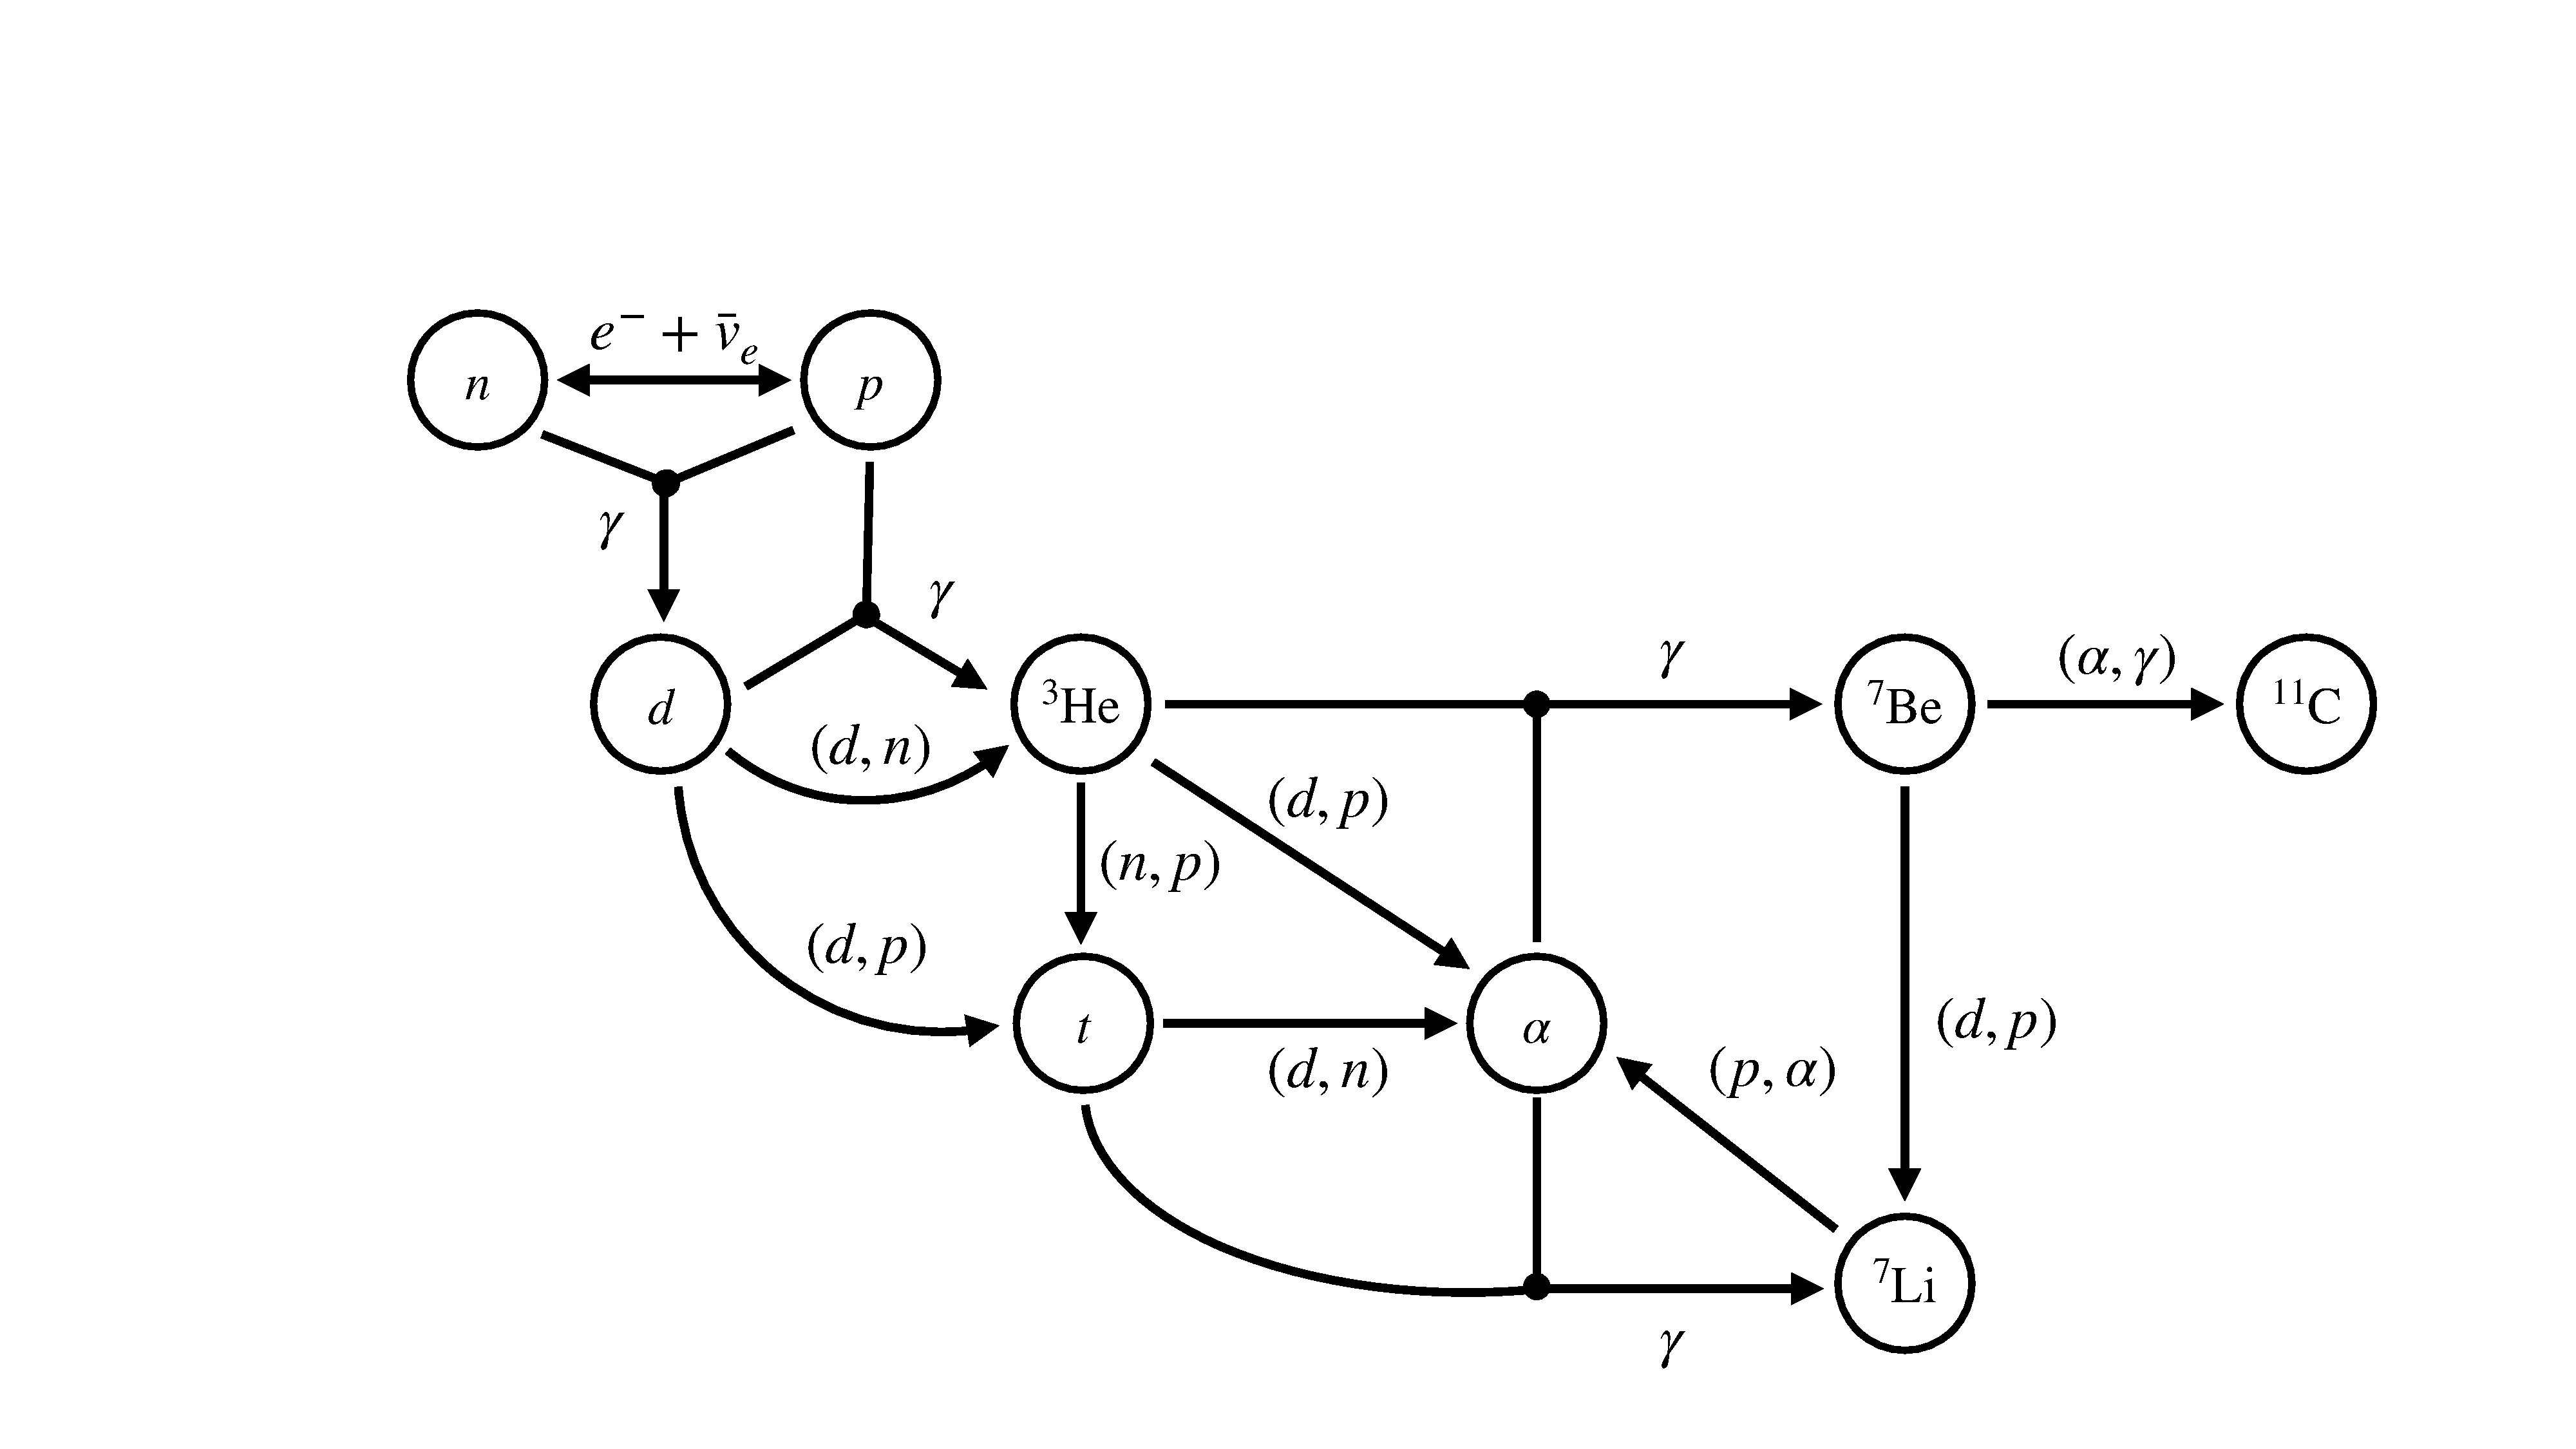
\includegraphics[scale=0.25]{Graphs/BBNchart.pdf}
	\caption[Nuclear reactions of Big Bang Nucleosynthesis]{Nuclear reactions of Big Bang Nucleosynthesis chart.}
	\label{fig:nuclearReactionsBNN}
\end{figure}


Furthermore, Big Bang nucleosynthesis can be extended beyond $\mathrm{Li}$ and $\mathrm{Be}$ to almost middle heavy production at very high temperatures \cite{wagoner_fowler_hoyle_1967}. Alternative processes use main products of the BBN reactions like $d$, $\mathrm{{}^{3}He}$, $\mathrm{{}^{4}He}$ or $\mathrm{{}^{7}Li}$ to produce heavier elements. For example, one of such reactions consists of successive alpha capture of $\mathrm{{}^{3}He}$ given by:


\begin{equation}\label{eq:reaction_BBN_chain}
	\mathrm{{}^{3}He({}^{4}He, \gamma){}^{7}Be({}^{4}He, \gamma){}^{11}C}.
\end{equation}

Alternatively, if enough lithium is available, $\mathrm{{}^{12}C}$ can be produced under specific conditions \cite{su-qing_kai-su_yong-shou_neng-chuan_zhi-hong_2010}. The chain involved begins with $\mathrm{{}^{8}{Li}}$ and requires $n$ capture and $(\alpha,n)$ exchange reactions to follow the process: 

\begin{equation}\label{eq:reaction_BBN_CNO_path}
	\mathrm{{}^{8}Li(n, \gamma){}^{9}Li(\alpha, n){}^{12}B(\beta){}^{12}C}.
\end{equation}

Appreciable heavier nuclei than $\mathrm{{}^{12}C}$ are not produced in the BBN framework. Instead, middle and heavy nuclei nucleosynthesis occur in stellar and explosive environments predominantly.


\section{Stellar fusion}  \label{sec:StellarFusion}

Much after the Big Bang, stars are formed through a process of gas accretion which forms environments with critical high temperatures and densities which allows the activation of fusion reactions for billions of years. During that period, stars remain stable due to the hydrostatic equilibrium established by the compensation of the compressing gravitational effect with the repulsive pressure exerted by fusion reaction produced radiation. In addition, stars are able to distribute their energy by maintaining convective heat exchanging mechanisms. \\

The diversity of the fusing nuclei at the core of stars heavily depends on their age and classification.  Initially, when the  temperature and density have just reached critical values,  hydrogen is the first element source of fusion reactions. Then, stars follow a sequence of nucleosynthesis processes which will produce heavier nuclei. A traditional survey of stellar fusion reactions is provided by the classical $\mathrm{B^{2}FH}$ paper \cite{burbidge_burbidge_fowler_hoyle_1957}. \\



In spite of the vast diversity of nucleosynthesis environments, a general classification of them is given by the categories encountered in the Hertzsprung-Russel (HR) diagram \cite{arsentieva_shevchenko_2021}.  Each category accounts for a region or cluster on the HR scatter plot with characteristic temperature and luminosity values for a certain stage in stellar evolution. The upcoming summary is based on the astrophysics textbook by Kundt \cite{kundt_2005}, further details should be consulted in that reference. \\

Brown dwarfs are the first of such classifications. These objects have a stellar magnitude which inhibited them to sustain a chain of hydrogen fusion. As a result, their luminosity is generally low. Their masses are roughly bounded by $M < 0.07M_{\odot}$. \\

Red dwarfs are the smallest objects which are able to sustain a chain of nuclear fusion reaction. Their color is red and their mass $ 0.07M_{\odot} < M < 0.5 M_{\odot} $ and low luminescence. Most of the stars on the Universe are in this group. However, at these mass values they are unable to burn helium \cite{kundt_2005}. \\

Main sequence branch, which is the current classification of the Sun, includes stars with middle mass with $ 0.5M_{\odot} < M < 2M_{\odot}$ approximately. Their color usually leans to yellow. They grow during their lives until they reach a red giant stage. \\

Asymptotic red giant is a superstar with the mass of $M > 2M_{\odot}$. They fuse $\mathrm{{}^{4}He}$ and even isotopes of carbon. Some stars of this kind release their material without explosion, like the case of the sun, while others are massive enough to collapse as a supernova given certain conditions which are going to be generally sketched later. In fact, it is critical to be annotated that mass is not the only criteria when determining the outcome of a star since variables like nuclear composition, density, angular momentum are eventually relevant.  \\

The supergiant and hypergiant are stars with high mass $M > 3M_{\odot}$ and gigantic size with radii $R \sim 1000R_{\odot}$. These stars are usually involved in highly explosive environments. One common kind is a IIA supernova, which is a mechanism of core collapse for stars that have reached iron as their ultimate product. On the other hand, a less common and more explosive example is a supernova of kind IA, which usually involve a binary system consistent of a red giant and a white dwarf. \\

White dwarfs are the remnants of the life of active stellar fusion. Their radius is close to the radius of the earth. Their stability is explained by repulsion degeneracy of their exterior layer of electrons. It is quite remarkable that this star is able to maintain hydrostatic equilibrium with mostly quantum-mechanical originated degeneracy pressure. Actually, these kinds of stars are critical for certain kinds of supernovae. \\ 

Neutron stars are compact objects which, like the white dwarfs, do not perform large-scale fusion sustainable reactions. Instead, their stability is explained by the repulsion generated by the fermionic degeneracy of their constituent neutrons. This explains the extremely compact nature of these objects since they are able to accumulate a mass comparable to that of the sun within a radius of a couple of tens of kilometers long. \\ 

Therefore, they are one of the most dense objects in the universe.  It has been speculated that  at the interior of these objects, a new state of matter, which is usually called the quark gluon plasma, is possible given the extreme conditions of degeneracy at these environments.\\ 

The next systems in compactness are black holes. These objects have self collapsed gravitationally to the point that even light cannot escape the gravitational binding at regions inside the event horizon. A first approach towards determining the mass limit of a star to become a black hole is known as the Chandasekar mass, which corresponds to 2.4 solar masses. However, a complete calculation should take into account particularities on the initial configuration of the star like its metallicity and element composition.  \\

\subsection{Light nuclei reactions} \label{sub:lightReactions}

Fusion reactions at stars start with hydrogen, which is originated from the Big Bang. Then, at the hot center of stars, a long chain of processes to produce $\mathrm{{}^{4}He}$, which is named as the pp chain, takes place.  Next, if stars have enough high temperatures, further heavy elements are produced from helium burning. This process is known as the triple alpha chain in where $\mathrm{{}^{12}C}$ and $\mathrm{{}^{16}O}$ nuclei are produced. Then, a series of cyclic reaction networks, which are referred to as CNO cycles, are present and expanded, for explosive and highly energetic environments, with the alternative  HCNO cycles. Finally, with most of the light nuclei produced, processes like $\Cfusion$ and $\Ofusion$, begin a new stage of nucleosynthesis ruled by middle heavy nuclei fusion.

\subsubsection{pp chain}

Much of the initial fusion at the core of a great extent of the lifetime of main branch stars like the sun consists of hydrogen fusion reactions. The interactions of pp-chain processes are mostly electromagnetic and strong force, with additional weak force mediated reactions. In addition, reaction rates of nuclear fusion processes depend on the interaction cross section and the abundance of the reactant nuclei. \\

The pp chain reactions and their connections are depicted in Figure \ref{fig:nuclerReactionppChain}

\begin{figure}[H]
	\centering 
	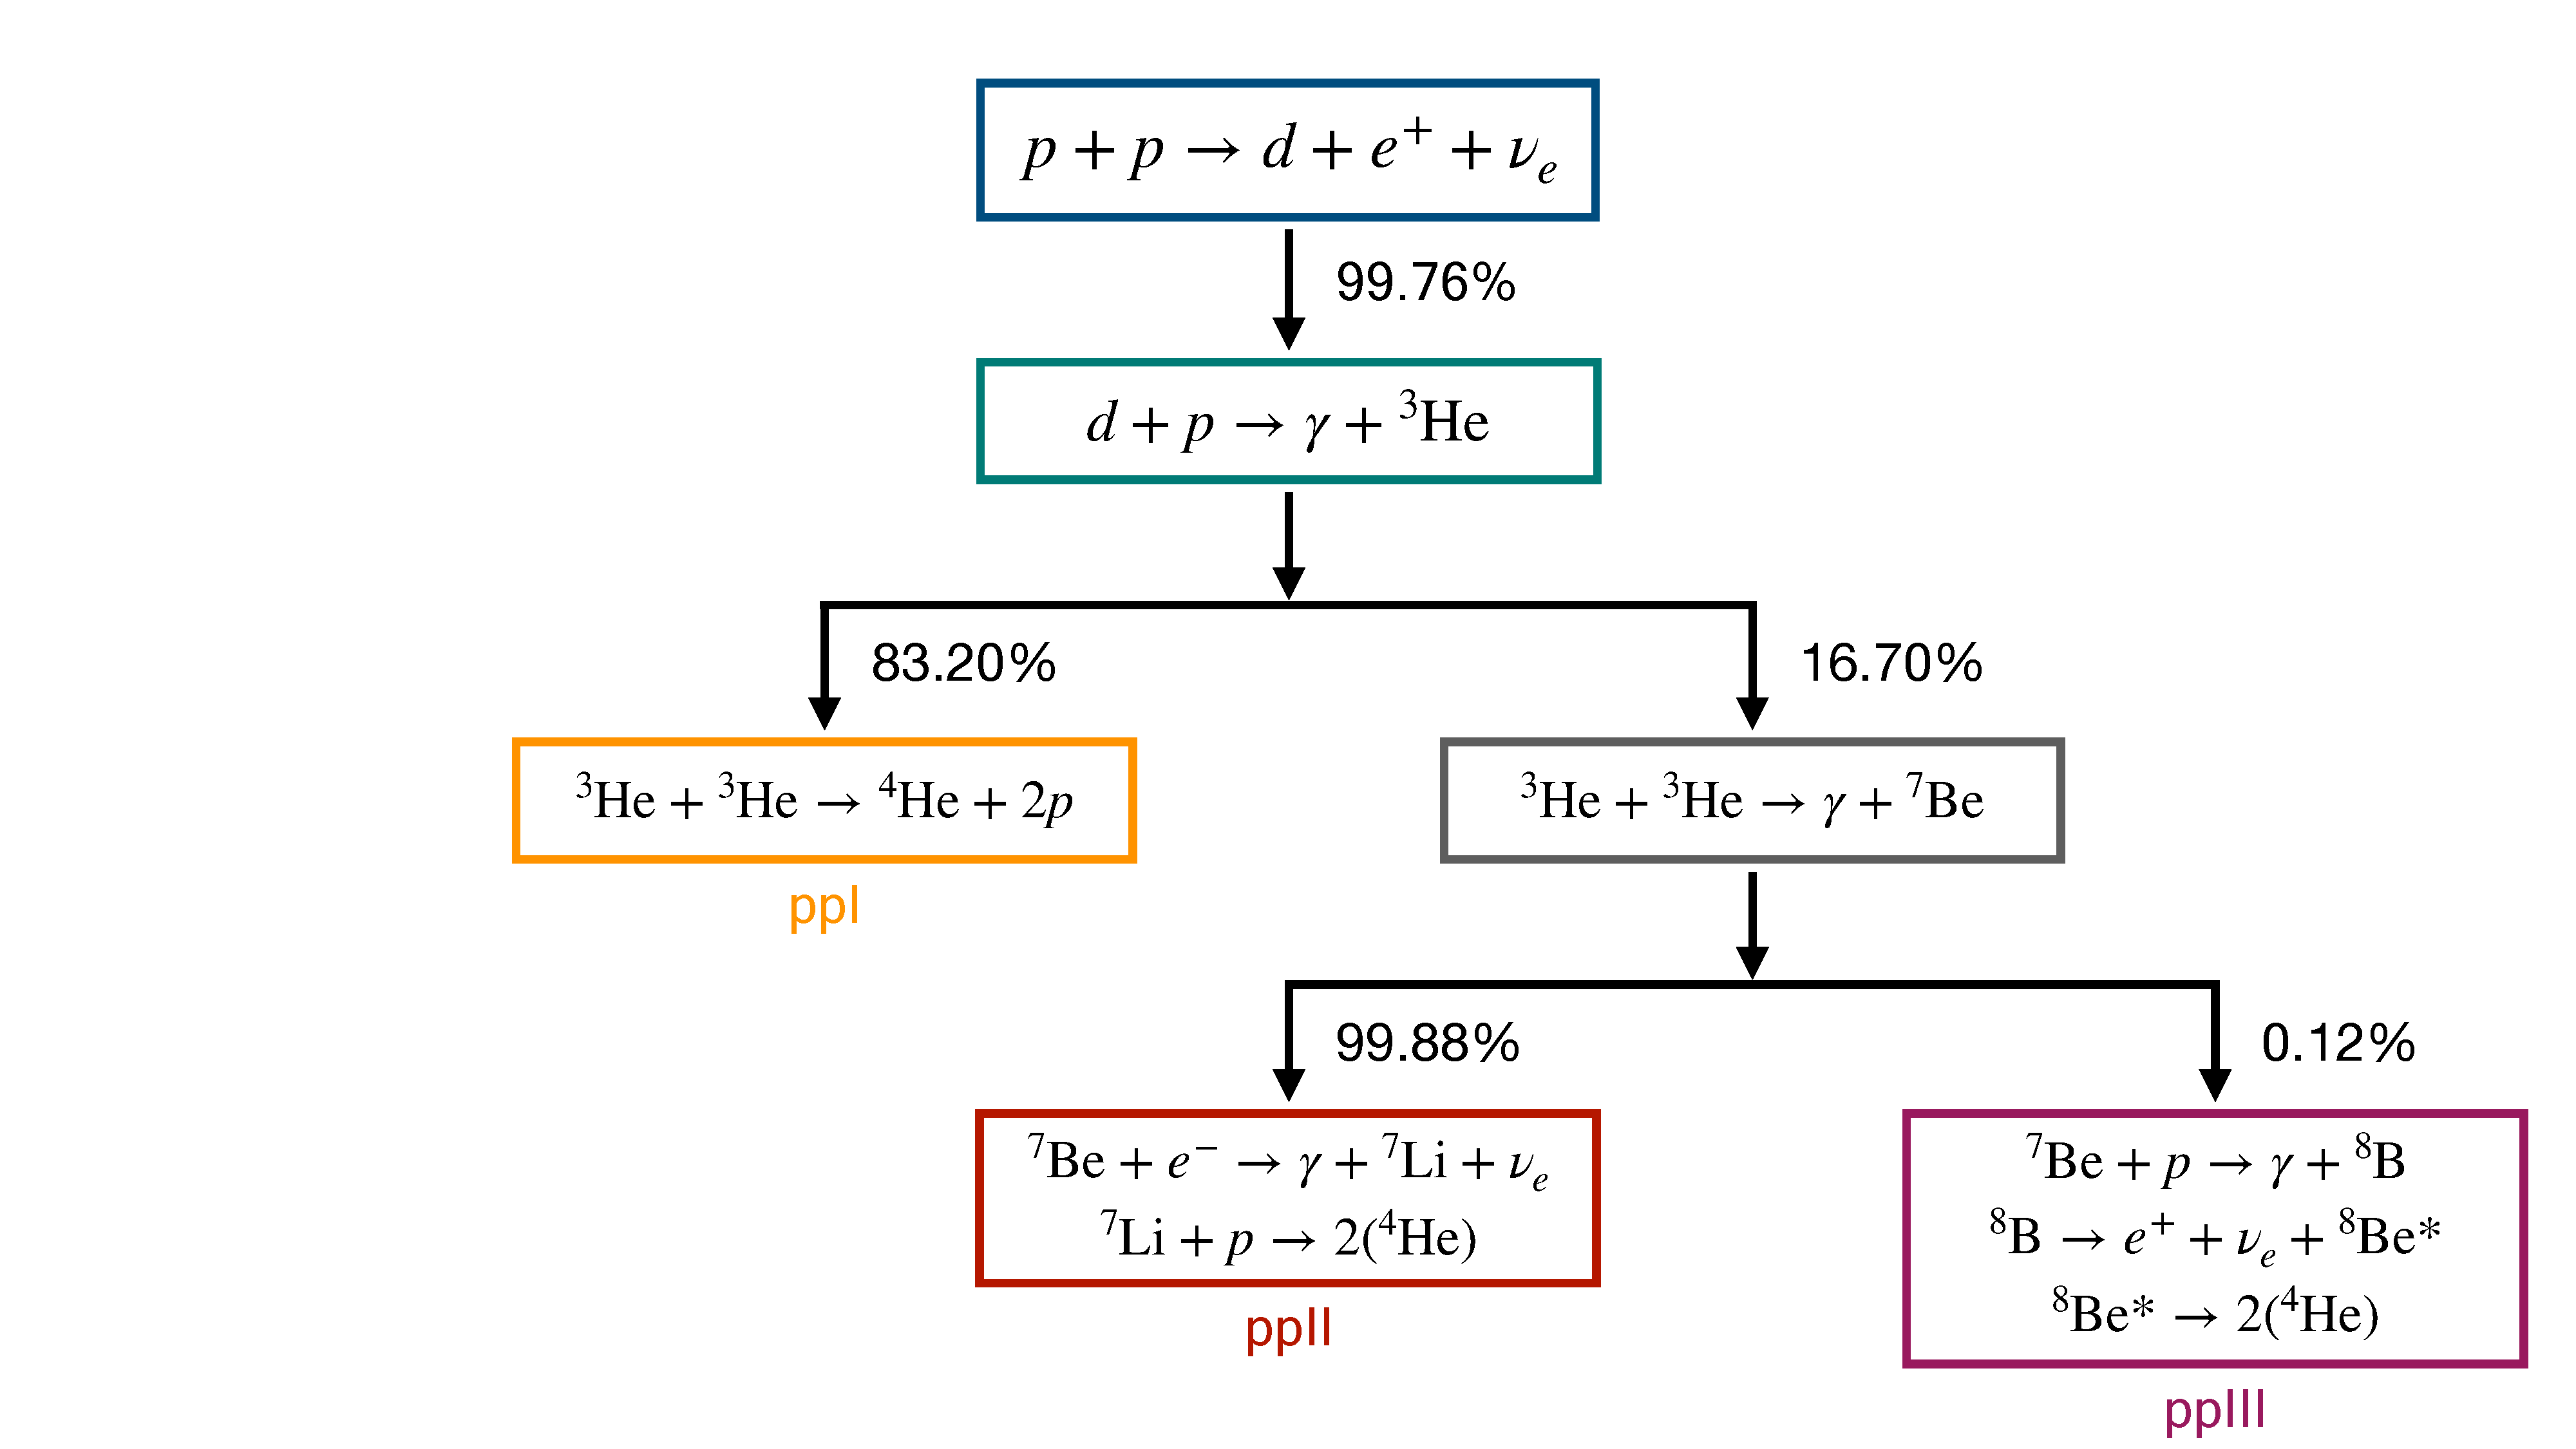
\includegraphics[scale=0.25]{Graphs/ppchart.pdf}
	\caption[Nuclear reactions of pp chain nucleosynthesis]{Nuclear reactions of pp chain nucleosynthesis. Probabilities were taken from \cite{bertulani_kajino_2016}.}
	\label{fig:nuclerReactionppChain}
\end{figure}


The initial reaction, which is the core process of hydrogen burning in stellar environments, proceeds as:  

\begin{equation} \label{eq:reaction_ppMain}
	p + p \rightarrow d + e^{+} + \nu_e.
\end{equation}

This first and critical pp reaction is mediated by the weak force. As a consequence of this fact, reaction times are long and therefore stars can sustain their stability driven by hydrostatic equilibrium for billions of years. Additionally, this reaction generates iirst synthesized nuclei of the chain, which is deuterium. \\

Then, when enough deuterium is available, a reaction to produce ${}^{3} \mathrm{He}$ follows. The exact form of this reaction is given by: 

\begin{equation} \label{eq:reaction_2Hpgamma3He}
	d + p  \rightarrow \gamma + {}^{3} \mathrm{He}.
\end{equation}

This reaction has the particularity of consuming $d$ very rapidly \cite{bertulani_2010}. Additionally, it opens three branches for the production of $\mathrm{{}^{4}He}$ due to ${}^{3} \mathrm{He}$ production \cite{fowler_1958}. The first branch (ppI) proceeds as by directly fusing $t$ as it is given by: 

\begin{equation} \label{eq:reaction_3Hep3He}
	 {}^{3} \mathrm{He} +  {}^{3} \mathrm{He} \rightarrow {}^{4}\mathrm{He} + 2p.
\end{equation}

The previous is the preferred process for stars at their initial stages since only $ {}^{3} \mathrm{He} $ is required. Alternatively, if a reasonable amount of ${}^{4}\mathrm{He}$ is present, stars may proceed with the two remaining branches of the pp chain with $\mathrm{{}^{7}Be}$ synthesis with the reaction: 

\begin{equation}  \label{eq:reaction_3He4He}
	{}^{3}\mathrm{He} +{}^{4}\mathrm{He} \rightarrow \gamma +  \mathrm{{}^{7}Be} .
\end{equation}

Subsequently, stars proceed with the second branch (ppII)  of the pp chain by synthesis of $\mathrm{{}^{7}Li}$ by means of electron capture, as it is given by:

\begin{equation}  \label{eq:reaction_7Beelectron}
	{}^{7}\mathrm{Be} + e^{-} \rightarrow \gamma +  \mathrm{{}^{7}Li} + \nu_e.
\end{equation}

Since a neutrino is produced, this reaction is also mediated by the weak force. Additionally, as it happens with pp initial process, reactions of equations \ref{eq:reaction_ppMain} and \ref{eq:reaction_7Beelectron} are key actors in solar neutrino production.  \\

Next, the second branch of the pp chain is completed with a predominantly nuclear mediated exchange reaction which involves a $(p, \alpha)$ process as given by: 

\begin{equation}  \label{eq:reaction_7Lialpha}
	{}^{7}\mathrm{Li} + p  \rightarrow 2\mathrm{{}^{4}He}.
\end{equation}

Since these nuclei are heavier than those on the first branch, $2\alpha$ were possible to be produced. Actually, a similar outcome is anticipated in the case of the third branch (ppIII). Instead of following the process of equation \ref{eq:reaction_7Beelectron}, the heavier $\mathrm{{}^{8}B}$ nucleus is produced by:

\begin{equation}  \label{eq:reaction_7Bep}
		{}^{7}\mathrm{Be}  + p \rightarrow \gamma +  \mathrm{{}^{8}B} .
\end{equation}

Then, a weak force mediated process leading to 2$\mathrm{{}^4He}$ production is given by: 

\begin{equation} \label{eq:reaction_8Bpositron}
	{}^{8}\mathrm{B} \rightarrow e^{+} + \nu_e + 	{}^{8}\mathrm{{Be}^{*}}.
\end{equation}

This process ends with an excited state ${}^{8}\mathrm{{Be}^{*}}$. Since this state is unstable and the $\mathrm{{}^{8}Be}$ nucleus can be modeled as a $2\alpha$ embedding, a cluster decay naturally follows as: 

\begin{equation} \label{eq:reaction_8Bdisintegration}
	{}^{8}\mathrm{{Be}^{*}} \rightarrow 2{}^{4}\mathrm{He}.
\end{equation}

The ppII is more unlikely than the ppIII chain \cite{bertulani_2010}. This might be explained by the fact that ppII proceeds in two  while ppIII in three steps. \\

As it is seen in the previous reactions, this chain ends with the production of $\mathrm{{}^{4}He}$. The chain stops here because this is the most stable nucleus of the light nuclei class. Additionally, this resulting nucleus is a relevant source of the production of heavier nuclei, in particular of the triple alpha process reactions. \\

\subsubsection{Triple alpha process}

When $\mathrm{{}^{4}He}$ abundance, as well as temperature and density conditions are sufficient to fuse helium, alpha capture processes take place. These conditions are not necessarily reached in all stars. In fact, the sun reaches this process at the last period of its lifetime. It is called triple alpha because it consists of three reactions involving $\alpha = \mathrm{{}^{4}He}$ particles \cite{coc_2012}. The initial of such reaction is:

\begin{equation}\label{eq:reaction_tripleAlpha_1}
	\mathrm{{}^{4}He + {}^{4}He \rightarrow  \gamma  + {}^{8}B}.
\end{equation}

Then, $\mathrm{{}^{8}B}$ it consumed by the next alpha capture with the form:

\begin{equation}\label{eq:reaction_tripleAlpha_2}
	\mathrm{{}^{8}B+ {}^{4}He \rightarrow  \gamma + {}^{12}C}. 
\end{equation}

Finally, the produced $\mathrm{{}^{12}C}$ nuclei can enter a CNO or HNCO cycle or capture an additional $\alpha$ with the reaction:

\begin{equation}\label{eq:reaction_tripleAlpha_3}
	\mathrm{{}^{12}C + {}^{4}He \rightarrow \gamma + {}^{16}O}.
\end{equation}

The resulting nuclei of this process is $\mathrm{{}^{16}O}$, which is a very stable since it is double magic. This reaction is completed with the production of another stable nuclei like $\mathrm{{}^{12}C}$. These two nuclei will have a substantial role in the production of heavier elements at the last stages of giant stars.

\subsection{CNO cycle}  \label{sub:CNOCycle}

When the star has capacity for completing the triple alpha process, their subproducts are available for additional nuclear reactions. In particular, with the presence of $\mathrm{{}^{12}C}$ nuclei, a series of capture reactions take place. These reactions conform the CNO cycle  \cite{wiescher_gorres_schatz_1999}. \\

The first cycle reactants include carbon, nitrogen and oxygen isotopes. The reaction proceeds as:  

\begin{equation} \label{eq:reaction_CNO_C}
	\mathrm{{}^{12}C  \rightarrow {}^{13}N  \rightarrow {}^{13}C  \rightarrow {}^{14}N  \rightarrow {}^{15}O  \rightarrow {}^{15}N \rightarrow {}^{12}C}.
\end{equation}

This fuels another nuclear capture cycle. In this case, the starting point are $\mathrm{{}^{14}N}$ nuclei and the cycle also involve oxygen and fluorine isotopes. In particular, the cycle is given explicitly by the reaction chain: 

\begin{equation} \label{eq:reaction_CNO_N}
	\mathrm{{}^{14}N  \rightarrow {}^{15}O \rightarrow {}^{15}N \rightarrow {}^{16}O  \rightarrow {}^{17}F  \rightarrow {}^{17}O  \rightarrow {}^{14}N}.
\end{equation}

There is even a third CNO cycle, which is far more uncommon and therefore is considerably less dominant than the second and first CNO cycle. In this case, the process is given by: 

\begin{equation} \label{eq:reaction_CNO_O}
	\mathrm{{}^{15}N  \rightarrow {}^{16}O  \rightarrow {}^{17}F \rightarrow {}^{17}O   \rightarrow {}^{18}F  \rightarrow {}^{18}O  \rightarrow {}^{15}N  }.
\end{equation}

All the previous cycles are coupled in the sense that the production of one element in one cycle may affect another cycle. In particular, CNOI fuels CNOII which at the same time feeds the CNOIII cycle. Particularly, Also notice that the three cycles begin with nuclei with consecutive atomic number. More concretely, carbon, nitrogen and oxygen nuclei begin the CNOI, CNOII and CNOIII cycles respectively.\\

There is also a CNOIV cycle, which is a version of the CNOIII with heavier nuclei. However, it is much less dominant than the CNOI cycle and relevant only in stellar fusion on heavy stars. The cycle is given by:

\begin{equation} \label{eq:reaction_CNO_O_4}
	\mathrm{{}^{16}O  \rightarrow {}^{17}F  \rightarrow {}^{17}O  \rightarrow {}^{18}F \rightarrow {}^{18}O   \rightarrow {}^{19}F  \rightarrow {}^{16}O  }.
\end{equation}


The last three processes are summarized in the illustration of Figure \ref{fig:CNOcyles}.


\begin{figure}[H]
	\centering 
	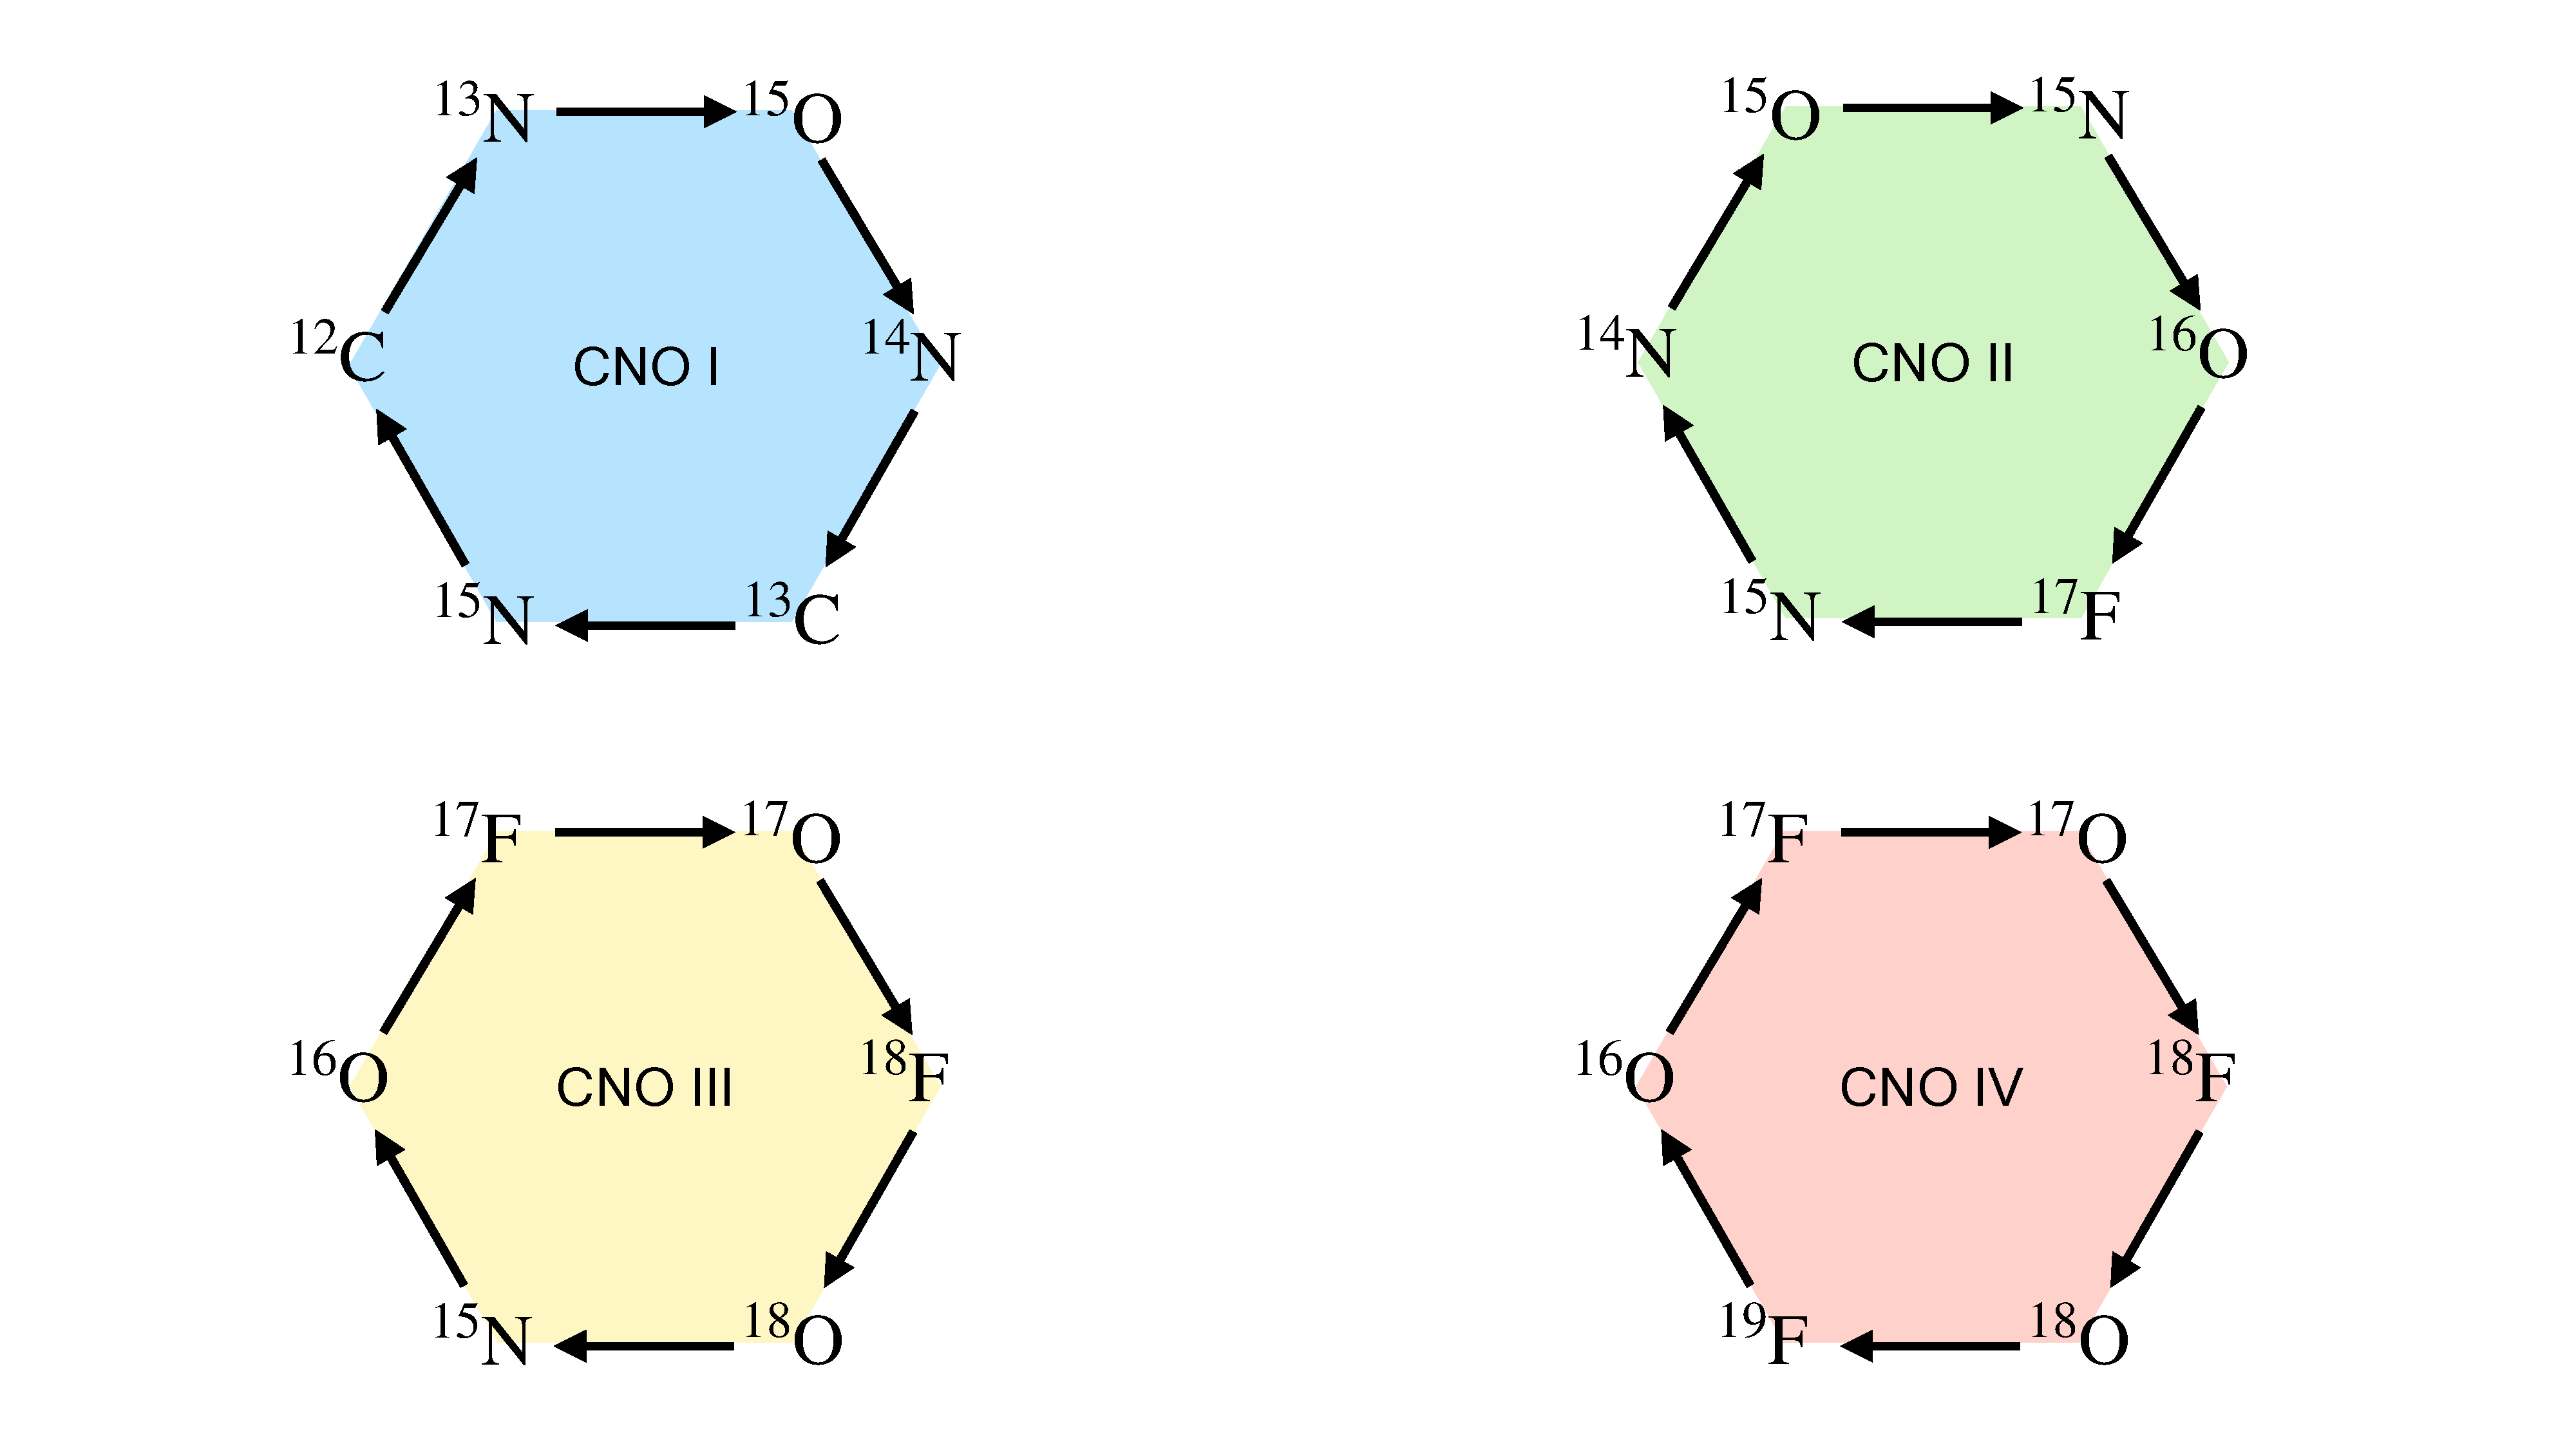
\includegraphics[scale=0.25]{Graphs/CNOchart.pdf}
	\caption[CNO I, II and III cycles representations]{CNO I, II and III cycles representations. Notice how products of the preceding cycles are sources of the next cycle. }
	\label{fig:CNOcyles}
\end{figure}


Notice that the cycle balance is established by the existence of proton capture and beta decay, which increases and decreases the atomic mass respectively. Then, any change in the rates of the previous reactions would alter the possibility of production of certain elements. In particular, at high enough temperatures, the rate of the proton capture process surpass that of the beta capture. Then, alternative products are synthesized and new processes form what is called hot CNO cycles. \\ 

At explosive environments, the CNO cycle is altered and it forms a new cyclic reaction chain called the HCNO cycle or hot CNO cycle.  New reactions are present given the more energetic conditions of this cycle. There are HCNOI, HCNOII and HCNOIII cycles, which are closely related with the CNOI, CNOII and CNOIII cycles respectively. For instance, the HCNOI proceeds as: 

\begin{equation} \label{eq:reaction_HCNO_C}
	\mathrm{{}^{12}C  \rightarrow {}^{13}N  \rightarrow \textcolor{blue}{{}^{14}O}  \rightarrow {}^{14}N  \rightarrow {}^{15}O  \rightarrow {}^{15}N \rightarrow {}^{12}C}.
\end{equation}

The colored term corresponds to the differing term in the cycle. Next, the HCNOII cycle is given by: 

\begin{equation} \label{eq:reaction_HCNO_N}
	\mathrm{{}^{15}N  \rightarrow {}^{16}O  \rightarrow {}^{17}F  \rightarrow \textcolor{blue}{{}^{18}Ne  \rightarrow {}^{18}F}  \rightarrow {}^{15}O \rightarrow {}^{15}N  }.
\end{equation}

The highlighted terms permit the cycle to reach a Ne isotope and are not present in the CNOII cycle. Lastly, the HCNO-III cycle proceeds like: 

\begin{equation} \label{eq:reaction_HCNO_O}
	\mathrm{{}^{16}O  \rightarrow {}^{17}F  \rightarrow {}^{18}Ne \rightarrow {}^{18}F  \rightarrow {}^{19}Ne  \rightarrow {}^{19}F \rightarrow {}^{16}O }.
\end{equation}

In contrast to the previous hot cycles, HCNOIII does not begin with the same nucleus as its non-hot analogue, the CNOIII cycle. Instead, it begins at $\mathrm{{}^{16}_{6}O}$ and, like the CNOIV cycle, is also able to produce neon nuclei in the process. \\

The previous hot HCNO cycles are represented in Figure \ref{fig:nuclerReactionppHCNO}.

\begin{figure}[H]
	\centering 
	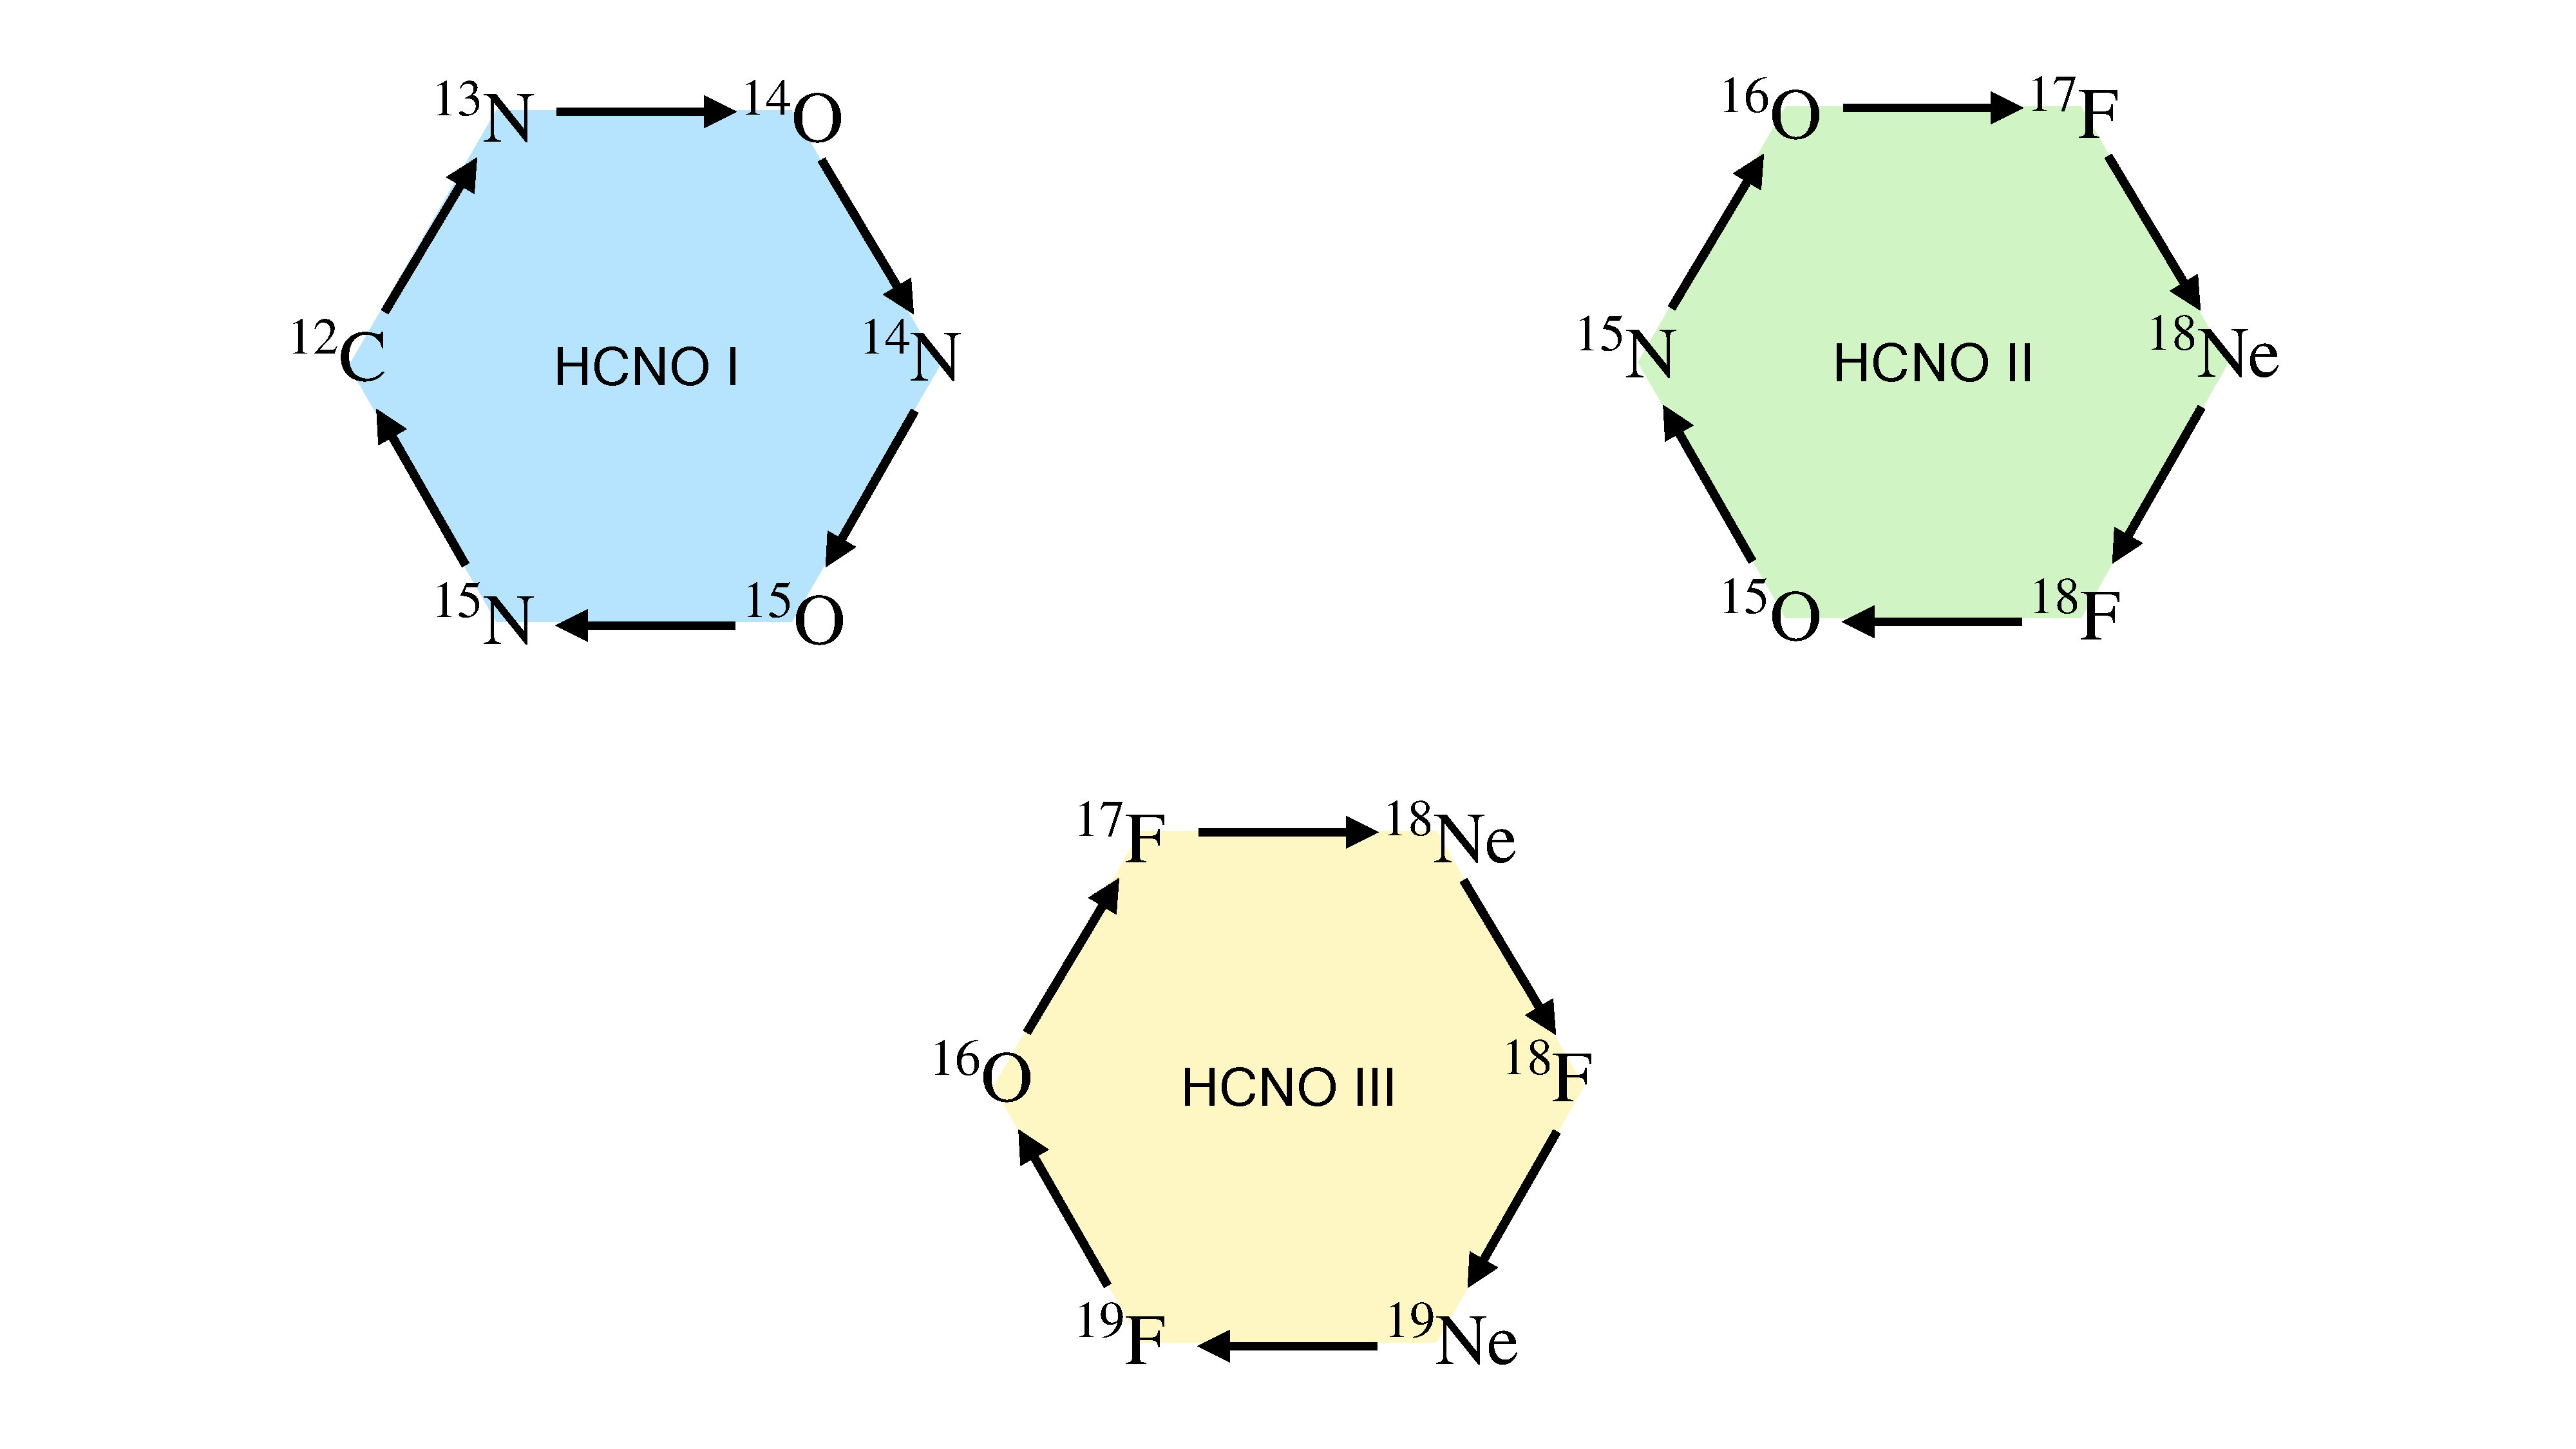
\includegraphics[scale=0.25]{Graphs/HCNOchart.pdf}
	\caption[Nuclear reactions of the HCNO cycles]{Nuclear reactions of the hot HCNO cycle.}
	\label{fig:nuclerReactionppHCNO}
\end{figure}

\subsection{Medium heavy nuclear reactions} \label{sub:mediumHeavyReactions}

When helium is on track of being consumed, temperatures and densities start to increase considerably as a consequence of stellar core contraction. Then, the fusion of middle heavy nuclei with $A < 28$, including carbon, neon, oxygen and silicon, occurs in different burning stages. During this period of time,  several nuclear reactions take place, which include the multi-channel $\mathrm{{}^{12}C + {}^{12}C}$ and $\mathrm{{}^{16}O + {}^{16}O}$ fusion reactions, as well the neon, magnesium, silicon reaction sequence. \\

\subsubsection{Carbon burning}\label{ssub:reactions_carbonBurning}

The first stage of middle heavy burning involves the $\mathrm{{}^{12}C}$ nucleus, which is synthesized in the triple alpha and the CNO processes. Given the high carbon abundance after helium is nearly exhausted, the star forms a carbon core which progressively transforms as the $\Cfusion$ reaction advances. There are three main channels for carbon fusion. The first is given by: 

\begin{equation} \label{eq:reaction_C12fusion_alpha20Ne}
	\mathrm{{}^{12}C + {}^{12}C \rightarrow {}^{4}He + {}^{20}Ne}. 
\end{equation}

It produces neon, which has a great relevance in further nucleosynthesis stages, and $\alpha$ particles. Alternatively, the second channel, which also produces neon, proceeds as:

\begin{equation} \label{eq:reaction_C12fusion_p23Ne}
	\mathrm{{}^{12}C + {}^{12}C \rightarrow p + {}^{23}Ne}. 
\end{equation}

In this case, a proton is released, and a new isotope of Ne is also produced. Lastly, carbon burning follows with the third channel, which is the magnesium producing reaction:

\begin{equation} \label{eq:reaction_C12fusion_n23Mg}
	\mathrm{{}^{12}C + {}^{12}C \rightarrow n  + {}^{23}Mg}. 
\end{equation}

The previous reactions illustrate how $\Cfusion$ is a source of $\alpha$, $n$ and $p$, which are essential ingredients of further nucleosynthesis processes like alpha capture, r-process and s-process. Additionally, the overall performance of the reaction considerably depends on temperature, the kind of solar model to be used and the alpha to proton ratio $R_\alpha/R_p$  \cite{pignatari_hirschi_wiescher_gallino_bennett_beard_fryer_herwig_rockefeller_timmes_et_2012}. \\

Another factor affecting the $\Cfusion$ reaction is its correlation with other fusion reactions involving $\mathrm{{}^{13}C}$ nuclei \cite{notani_esbensen_fang_bucher_davies_jiang_lamm_lin_ma_martin_et_2012}. Particularly, it is possible to constraint cross section values of the $\Cfusion$ reaction with an analysis on the $\mathrm{{}^{12}C + {}^{13}C}$ reaction \cite{zhang_wang_tudor_bucher_burducea_chen_chen_chesneanu_chilug_gasques_et_2020}. This comparison in viable given the similarities of the resonances present in the cross sections of the aforementioned reactions. For example, one of the main  neon producing channel of the $\mathrm{{}^{12}C + {}^{13}C}$ is given by: 

\begin{equation}\label{eq:middleFusion_12C13C}
	\mathrm{{}^{12}C + {}^{13}C \rightarrow p + {}^{24}Na}.
\end{equation} 

\subsubsection{Oxygen burning}\label{ssub:reactions_oxygenBurning}

Later, oxygen starts to burn after carbon and neon. A key fact to explain this delay is that oxygen is a very stable nucleus given its double magic property. Massive stars ranging 15 to 30 $M_{\odot}$ are ideal environments to produce oxygen burning at their cores. Most $\mathrm{{}^{16}O}$ nuclei are produced by the triple alpha $\mathrm{{}^{12}C(\alpha, \gamma){}^{16}O}$ reaction involving carbon. Additionally, some ratios of nuclei like  $\mathrm{{}^{12}C/{}^{13}C}$, $\mathrm{{}^{14}N/{}^{15}N}$, $\mathrm{{}^{16}O/{}^{17}O}$,  $\mathrm{{}^{16}O/{}^{18}O}$, and $\mathrm{Na/Fe}$ impact the performance of the oxygen fusion reaction \cite{eleid_meyer_the_2004}. \\

As it happens with the $\Cfusion$ case, $\Ofusion$ has associated several channels. One relevant channel of the oxygen fusion reaction occurs in the following manner:

\begin{equation} \label{eq:reaction_O16fusion_alpha28Si}
	\mathrm{{}^{16}O + {}^{16}O \rightarrow {}^{4}He + {}^{28}Si}. 
\end{equation}

A key feature of this channel is the production of the $\mathrm{{}^{28}Si}$ which will be critical for the silicon burning process. Alternatively, the neutron producing channel related to oxygen burning, which is analogous to the reaction of equation \ref{eq:reaction_C12fusion_n23Mg}, proceeds as: 

\begin{equation} \label{eq:reaction_O16fusion_n31S}
	\mathrm{{}^{16}O + {}^{16}O \rightarrow n + {}^{31}S}. 
\end{equation}

Additionally, as it happens with the reaction of equation \ref{eq:reaction_C12fusion_p23Ne}, the proton releasing channel is relevant and proceeds like: 

\begin{equation} \label{eq:reaction_O16fusion_p31P}
	\mathrm{{}^{16}O + {}^{16}O \rightarrow p + {}^{31}O}. 
\end{equation}

As it was anticipated earlier, there are more carbon and oxygen fusion reactions than the previously mentioned. A larger picture with most of the channels involved in carbon and oxygen fusion reactions is represented in Figure \ref{fig:COchannels}. The entire spectrum involves a wide list of products in which $\alpha$, $n$, $p$ and $2p$, $2\alpha$, $\alpha p$, $\alpha n$ are included. In the case of oxygen, the channels are given by \cite{kuronen_keinonen_tikkanen_1987}:  

\begin{equation}\label{eq:middleFusion_experimental_16O16O_channels}
	\begin{split}
		\Ofusion &\rightarrow \mathrm{n + {}^{31}S} \\
		&\rightarrow \mathrm{p + {}^{31}P} \\
		&\rightarrow \mathrm{\alpha + {}^{28}Si} \\
		&\rightarrow \mathrm{2p + {}^{30}Si} \\
		&\rightarrow \mathrm{\alpha + p + {}^{27}Al} \\
		&\rightarrow \mathrm{2\alpha + {}^{24}Mg} \\
		&\rightarrow \mathrm{n + p + {}^{30}P}. \\
	\end{split}
\end{equation}

Middle heavy fusion reactions have in common Coulomb barriers in the range of MeV. Additionally, at energies beyond the barrier, it is usual to encounter an almost non-resonant behavior in the cross sections. However, as the energy decreases, the effects of nuclear structure are more noticeable. Particularly, molecular effects are relevant since various degrees of freedom like rotation or vibration are allowed. Therefore, new possible transitions enhance reaction probabilities. \\

In order to account for new degrees of freedom, clustering is used for modeling these nuclei. For example, $\mathrm{{}^{12}C}$ can be interpreted as a $3\alpha$ cluster. Similarly, the $\mathrm{{}^{16}O}$  has a structure of a $4\alpha$ wrapper. Then, nuclear attraction can be represented by nucleon-nulceon, or alternatively cluster-cluster interactions. The former is privileged when calculations are performed with all the nucleons while the latter assumes an effective interaction among the constituent alpha particles of the nuclei.  \\

\begin{figure}[H]
	\begin{center}
	\begin{tikzpicture}

		\node (center) at (0, 0) {$\mathrm{{}^{16}O + {}^{16}O}$};
		
		%\node (CH1) at (6, 3) {$\mathrm{{}^{4}He + {}^{28}Si}$};
		%\node (CH2) at (3, 3) {$\mathrm{p + {}^{31}P}$};
		%\node (CH3) at (0, 3) {$\mathrm{d + {}^{30}P}$};
		%\node (CH4) at (-3, 3) {$\mathrm{\alpha \alpha + {}^{30}P}$};
		%\node (CH5) at (-6, 3) {$\mathrm{n + {}^{31}{S}}$ };
		
		\node (CH1) at (3, 6) {$\mathrm{\alpha + {}^{28}Si}$};
		\node (CH2) at (3, 3) {$\mathrm{p + {}^{31}P}$};
		\node (CH3) at (3, 0) {$\mathrm{d + {}^{30}P}$};
		\node (CH4) at (3, -3) {$\mathrm{\alpha \alpha + {}^{30}P}$};
		\node (CH5) at (3, -6) {$\mathrm{n + {}^{31}{S}}$ };
		
		\draw[-stealth] (center) -- (CH1);
		\draw[-stealth] (center) -- (CH2);
		\draw[-stealth] (center) -- (CH3);
		\draw[-stealth] (center) -- (CH4);
		\draw[-stealth] (center) -- (CH5);
		
		\node (center2) at (10, 0) {$\mathrm{{}^{12}C + {}^{12}C}$};
		
		\node (CH6) at (13, 6) {$\mathrm{\alpha + {}^{20}Ne}$};
		\node (CH7) at (13, 3) {$\mathrm{p + {}^{23}Na}$};
		\node (CH8) at (13, 0) {$\mathrm{d + {}^{22}Na}$};
		\node (CH9) at (13, -3) {$\mathrm{\alpha \alpha + {}^{16}O}$};
		\node (CH10) at (13, -6) {$\mathrm{n + {}^{23}{Mg}}$ };
		
		\draw[-stealth] (center2) -- (CH6);
		\draw[-stealth] (center2) -- (CH7);
		\draw[-stealth] (center2) -- (CH8);
		\draw[-stealth] (center2) -- (CH9);
		\draw[-stealth] (center2) -- (CH10);
		
	\end{tikzpicture}
\end{center}

	\caption[Carbon and oxygen burning main channels.]{Reaction chart of carbon and oxygen burning channels.}
	\label{fig:COchannels}
\end{figure}

The $\Ofusion$ is not the only oxygen fusion reaction.  Isotopes $\Ofusion[16][17]$, $\Ofusion[16][18]$ also make an impact in the production of heavier elements, as it was anticipated earlier, and in constraining the $\Ofusion$ reaction. Additionally, $\Ofusion[16][17]$, $\Ofusion[16][18]$ also present many channels. Some of them are listed as \cite{thomas_chen_hinds_meredith_olson_1986}: 

\begin{equation}\label{eq:middleFusion_experimental_16O17O_channels}
	\begin{split}
		\Ofusion[16][17]  & \rightarrow \mathrm{n + {}^{32}S} \\
		&\rightarrow \mathrm{p + {}^{32}P} \\
		&\rightarrow \mathrm{\alpha + {}^{29}Si} \\
		&\rightarrow \mathrm{2n + {}^{31}S} \\
		&\rightarrow \mathrm{2p + {}^{31}Si} \\
		&\rightarrow \mathrm{\alpha + p + {}^{28}Al} \\
		&\rightarrow \mathrm{2\alpha + {}^{25}Mg} \\
		&\rightarrow \mathrm{n + p + {}^{31}P}. \\
	\end{split}
\end{equation}

Reciprocally, the latter is related with reactions like the following:

\begin{equation}\label{eq:middleFusion_experimental_16O18O_channels}
	\begin{split}
		\Ofusion[16][18] &\rightarrow \mathrm{n + {}^{33}S} \\ 
		&\rightarrow \mathrm{p + {}^{33}P} \\
		&\rightarrow \mathrm{\alpha + {}^{30}Si} \\
		&\rightarrow \mathrm{2n + {}^{32}S} \\
		&\rightarrow \mathrm{2p + {}^{32}Si} \\
		&\rightarrow \mathrm{2p + n + {}^{31}Si} \\
		&\rightarrow \mathrm{\alpha + p + {}^{29}Al} \\
		&\rightarrow \mathrm{\alpha + n + {}^{29}Si} \\
		&\rightarrow \mathrm{2\alpha + {}^{26}Mg} \\
		&\rightarrow \mathrm{n + p + {}^{32}P} \\
		&\rightarrow \mathrm{2n + p + {}^{31}P}. \\
	\end{split}
\end{equation}

A key feature of these alternative reactions is that they have associated elastic and inelastic states. For example, channels involving excited $\mathrm{{}^{18}O^{*}}$ nuclei could increase the cross section of the reaction of equation \ref{eq:middleFusion_experimental_16O18O_channels}.  \\

Additionally, as carbon and oxygen can react while coexisting in a certain period of stellar nucleosynthesis. The $\mathrm{{}^{12}C + {}^{16}O}$ reaction is a classical example. In fact, this process shares with $\Cfusion$ the distinct feature of presenting resonances at energies below the Coulomb barrier \cite{torilov_maltsev_zherebchevsky_2021}. These gross structures can be studied with the information of the alternative reaction $\mathrm{{}^{12}C + {}^{18}O}$ \cite{chan_bohn_vandenbosch_sielemann_cramer_bernhardt_bhang_chiang_1979}, which can be interpreted to have an analogous role to the $\mathrm{{}^{12}C + {}^{13}C}$ reaction in the study of $\Cfusion$ resonances. A general treatment of the cross section of these reactions is given by 
superimposing the resonant and non-resonant contributions. Namely, 

\begin{equation}\label{eq:middleFusion_sumResonantNonResonant}
	\sigma^{(\mathrm{tot})} = \sigma^{(\mathrm{res})} + \sigma^{(\mathrm{non-res})},
\end{equation}

where $\sigma^{(\mathrm{res})}$ and $\sigma^{(\mathrm{non-res})}$ are the resonant and non-resonant cross sections respectively. \\

Additionally, like in the case of the previously reviewed middle heavy fusion reactions, $\mathrm{{}^{12}C + {}^{16}O}$ is a multi-channel reaction with the form:

\begin{equation}\label{eq:middleFusion_experimental_12C18O_channels}
	\begin{split}
		\mathrm{{}^{12}C + {}^{16}O} &\rightarrow \mathrm{p + {}^{27}Al} \\
		&\rightarrow \mathrm{2p + {}^{26}Mg} \\
		&\rightarrow \mathrm{\alpha + 2p + {}^{22}Ne} \\
		&\rightarrow \mathrm{\alpha  + {}^{24}Mg} \\
		&\rightarrow \mathrm{n + 2p + {}^{25}Mg} \\
		&\rightarrow \mathrm{\gamma + {}^{28}Si}. \\
	\end{split}
\end{equation}

Notice that, like $\Cfusion$ and $\Ofusion$, alpha particles, protons and neutrons were produced, in addition to neon and magnesium isotopes which permit the continuation of nucleosynthesis of heavier elements. 

\subsubsection{Neon, magnesium and silicon burning} \label{ssub:reactions_neonMagnesiumSiliconBurning}

After carbon is exhausted, neon burning proceeds. A key difference with both carbon and oxygen is that neon does not present a direct Ne - Ne reaction with multiple channels. The high Coulomb barrier is a central reason why direct fusion is unlikely. Instead, It comprehends various reactions to obtain a net fusion reaction which involves magnesium. One of the main sources of neon, as well as magnesium, comes by extending the tripe alpha process as \cite{kaeppeler_wiescher_giesen_goerres_baraffe_eleid_raiteri_busso_gallino_limongi_et_1994}:

\begin{equation}\label{eq:reaction_4chain}
	\mathrm{{}^{12}C(\alpha, \gamma){}^{16}O(\alpha, \gamma){}^{20}Ne(\alpha, \gamma){}^{24}Mg.}
\end{equation}

$\mathrm{{}^{20}Ne}$ is the main Ne nuclei which is produced from the extended triple alpha $\mathrm{{}^{16}O(\alpha, \gamma){}^{20}Ne}$ reaction. Additionally, it is also included as a subproduct of $\Cfusion$ burning. It also $\alpha$-decays back to oxygen with the inverse $\mathrm{{}^{20}Ne(\alpha, \gamma){}^{16}O}$ reaction. Conversely, it also contributes with an $\alpha$ capture to produce $\mathrm{{}^{24}Mg}$. Additionally, the $\mathrm{{}^{23}Na}$, a product of $\Cfusion$, is also involved in neon burning. It produces the former and $\mathrm{{}^{26}Mg}$ via $(p, \alpha)$ and $(p, \alpha)$ processes respectively. A summary of the previously stated reactions relevant to the Ne process are listed as \cite{arnett_1974}:

\begin{equation}\label{eq:reaction_neon_processes}
	\begin{split}
		\mathrm{{}^{23}Na(\alpha, p){}^{26}Mg}, \\
		\mathrm{{}^{23}Na(p, \alpha){}^{20}Ne}, \\
		\mathrm{{}^{20}Ne(\alpha, \gamma){}^{24}Mg}, \\ 
		\mathrm{{}^{20}Ne(\gamma, \alpha){}^{16}O}.
	\end{split}
\end{equation}

Two main conclusions can be inferred from the previous lines. On the one hand, the net $\mathrm{{}^{20}Ne + {}^{20}Ne}$, which involves the last two reactions, is founded to be: 

\begin{equation}\label{eq:reaction_neon_net}
	\mathrm{{}^{20}Ne + {}^{20}Ne \rightarrow {}^{24}Mg + {}^{16}O}.
\end{equation}

On the other hand, a simplified alternative which condenses the previous reactions, without considering $\alpha$, $p$ and $\gamma$, is obtained by adjusting stoichiometric coefficients to get a net reaction with the form: 

\begin{equation}\label{eq:reaction_sodium_net}
	\mathrm{4{}^{23}Na \rightarrow 2 {}^{26}Mg + {}^{24}Mg + {}^{16}O}.
\end{equation}

Then, neon burning produces the two magnesium isotopes $\mathrm{{}^{26}Mg}$ and $\mathrm{{}^{24}Mg}$. A key aspect that the last nuclei have in common is their involvement in the MgAl cycle. This process takes place on asymptotic branch stars, massive stars and novae. Initially, $\mathrm{{}^{25}Mg}$ nucleus reacts to produce $\mathrm{{}^{26}Al}$ by the process $\mathrm{{}^{25}Mg(p, \gamma){}^{26}Al}$. Alternatively, $\mathrm{{}^{24}Mg}$ is also a source of $\mathrm{{}^{26}Al}$ by the process $\mathrm{{}^{24}Mg({}^{3}He, p){}^{26}{Al}}$. Then $\mathrm{{}^{26}Al}$, which is related to an unlikely long-lived isotope associated with an isomer state,  $\beta^{+}$ decays back to magnesium and particularly to the isotope $\mathrm{{}^{26}Mg}$ \cite{lotay_doherty_janssens_seweryniak_albers_almaraz-calderon_carpenter_champagne_chiara_hoffman_et_2022}. \\

Additionally, $ \mathrm{{}^{24}Mg}$ contributes to the production of silicon by the capture reaction: 

\begin{equation}\label{eq:reaction_magnesium_alphaCapture}
		\mathrm{{}^{24}Mg + \alpha \leftrightarrow {}^{28}Si + \gamma}.
\end{equation}

Silicon burning is another process that bridges middle to heavy nucleosynthesis. As it is the case of the last reaction, the main process is an alpha capture with the form \cite{bodansky_clayton_fowler_1968}:   \\

\begin{equation} \label{eq:reaction_28Sialpha}
	\mathrm{{}^{28}Si +{}^{4}He \rightarrow {}^{32}S + \gamma}.
\end{equation}

However, rather than a forward reaction, an equilibrium is established by considering also the reciprocal photodisintegration process:

\begin{equation}\label{eq:reaction_S_equillibrium}
	\mathrm{{}^{32}S + \gamma \rightarrow  {}^{28}Si+ \alpha}.
\end{equation}

It is to be noticed that, in sharp contrast with $\Cfusion$ and $\Ofusion$ reactions, as well to a minor extent with the net neon burning of equation \ref{eq:reaction_neon_net}, the fusion reaction

\begin{equation} \label{eq:reaction_28Sifusion_alpha56Fe}
	\mathrm{{}^{28}Si + {}^{28}Si \rightarrow {}^{4}He + {}^{52}Fe }
\end{equation}

is generally not viable in a single step at stellar conditions mainly due to the high Coulomb barrier which effectively avoids the process to be considerable. Instead, it would actually take several alpha capture steps to produce $\mathrm{{}^{52}Fe}$ as it will be observed in the next section. \\

As there is carbon coexisting with Si and Mg nuclei, scattering reactions $\mathrm{{}^{12}C + {}^{24}Mg}$ as well as in the $\mathrm {{}^{12}C + {}^{30}Si}$ might occur with a characteristic maximum of the S-factor at energies of astrophysical interest \cite{montagnoli_stefanini_jiang_colucci_goasduff_brugnara_mazzocco_siciliano_scarlassara_corradi_et_2020}.


\section{Heavy nuclei reactions} \label{sec:heavyReactions}

After carbon, oxygen, neon and silicon combustion are over, heavier elements with $A > 28$ are produced at the last stages of the life of a star. Depending on the astrophysical context, they may be synthesized by extended reaction chains, which ultimately ends with iron core formation in massive stars, or in explosive environments like supernovae or high energy X-ray events, which are ideal scenarios for the production of the  heaviest elements in the Universe. In this section, a special emphasize is given to the production of $\mathrm{{}^{52}Fe}$ through alpha capture and related reactions within stellar fusion context. Additionally, the critical neutron capture s and r processes will be reviewed, with their analogous p and rp in the case of proton capture will be analyzed. 

\subsection{Alpha reactions} \label{sub:alphaProcesses}

Initially, as it was reviewed in previous sections, when $\alpha$ fusion become possible, and if sufficient conditions are given, the triple alpha fusion reaction, which ends in the production of $\mathrm{{}^{16}O}$, starts. Then, after the silicon burning stage, $\mathrm{{}^{28}Si}$ synthesis is reached by similar alpha capture means. Next, alpha reactions acquire a relevant role in increasing the mass number of nuclei. A chain of alpha capture reactions, which is usually referred to as the alpha ladder, is given by the sequence of reactions:

\begin{equation}  \label{eq:reaction_alphaLatter}
	\mathrm{{}^{28}Si \rightarrow {}^{32}S \rightarrow {}^{36}Ar \rightarrow {}^{40}Ca \rightarrow {}^{44}Ti  \rightarrow {}^{48} Cr \rightarrow {}^{52}Fe}.
\end{equation}

In order to produce heavy nuclei by this process, captures must dominate photodisintegrations, which are increasingly favored as the chain advances due to the accumulation of emitted photons which were produced on each step of the alpha capture chain. Eventually, photodisintegration overcomes alpha capture when the chain completes the process:

\begin{equation}  \label{eq:reaction_52Fealpha}
	\mathrm{{}^{52}Fe +{}^{4}He \rightarrow {}^{56}Ni} + \gamma.
\end{equation}

Later, when $\mathrm{{}^{56}Ni}$ nuclei are produced, it is no longer viable to keep the chain going due to the excess of photodisintegration events. Beyond that peak, it is more likely that a nucleus would disintegrate via alpha or cluster decay. Then, as  $\mathrm{{}^{56}Ni}$ decays to $\mathrm{{}^{56}Fe}$, the last core of stars, made by iron, is formed. Since iron burning is not viable, stellar hydrostatical equilibrium is no longer sustainable and, in the great majority of cases, an explosive event imperatively follows. \\

However, reactions involving alpha particles are not limited to alpha capture or decay. Other exchange reactions which increases $(\alpha, n), (\alpha, p)$ and decreases $(p, \alpha), (n, \alpha)$ the mass number take place in nucleosynthesis. Additionally, if certain stability and environmental conditions are given,  it is possible to find processes involving double alpha absorption and emission  Namely, $(\alpha \alpha, n)$, $(\alpha \alpha, p)$, $(\alpha \alpha, \gamma)$ and $(n, \alpha \alpha), (p, \alpha \alpha), (\gamma, \alpha \alpha)$ respectively. All of them are summarized in Figure \ref{fig:alphaChart}.

\begin{figure}[H]
	\centering 
	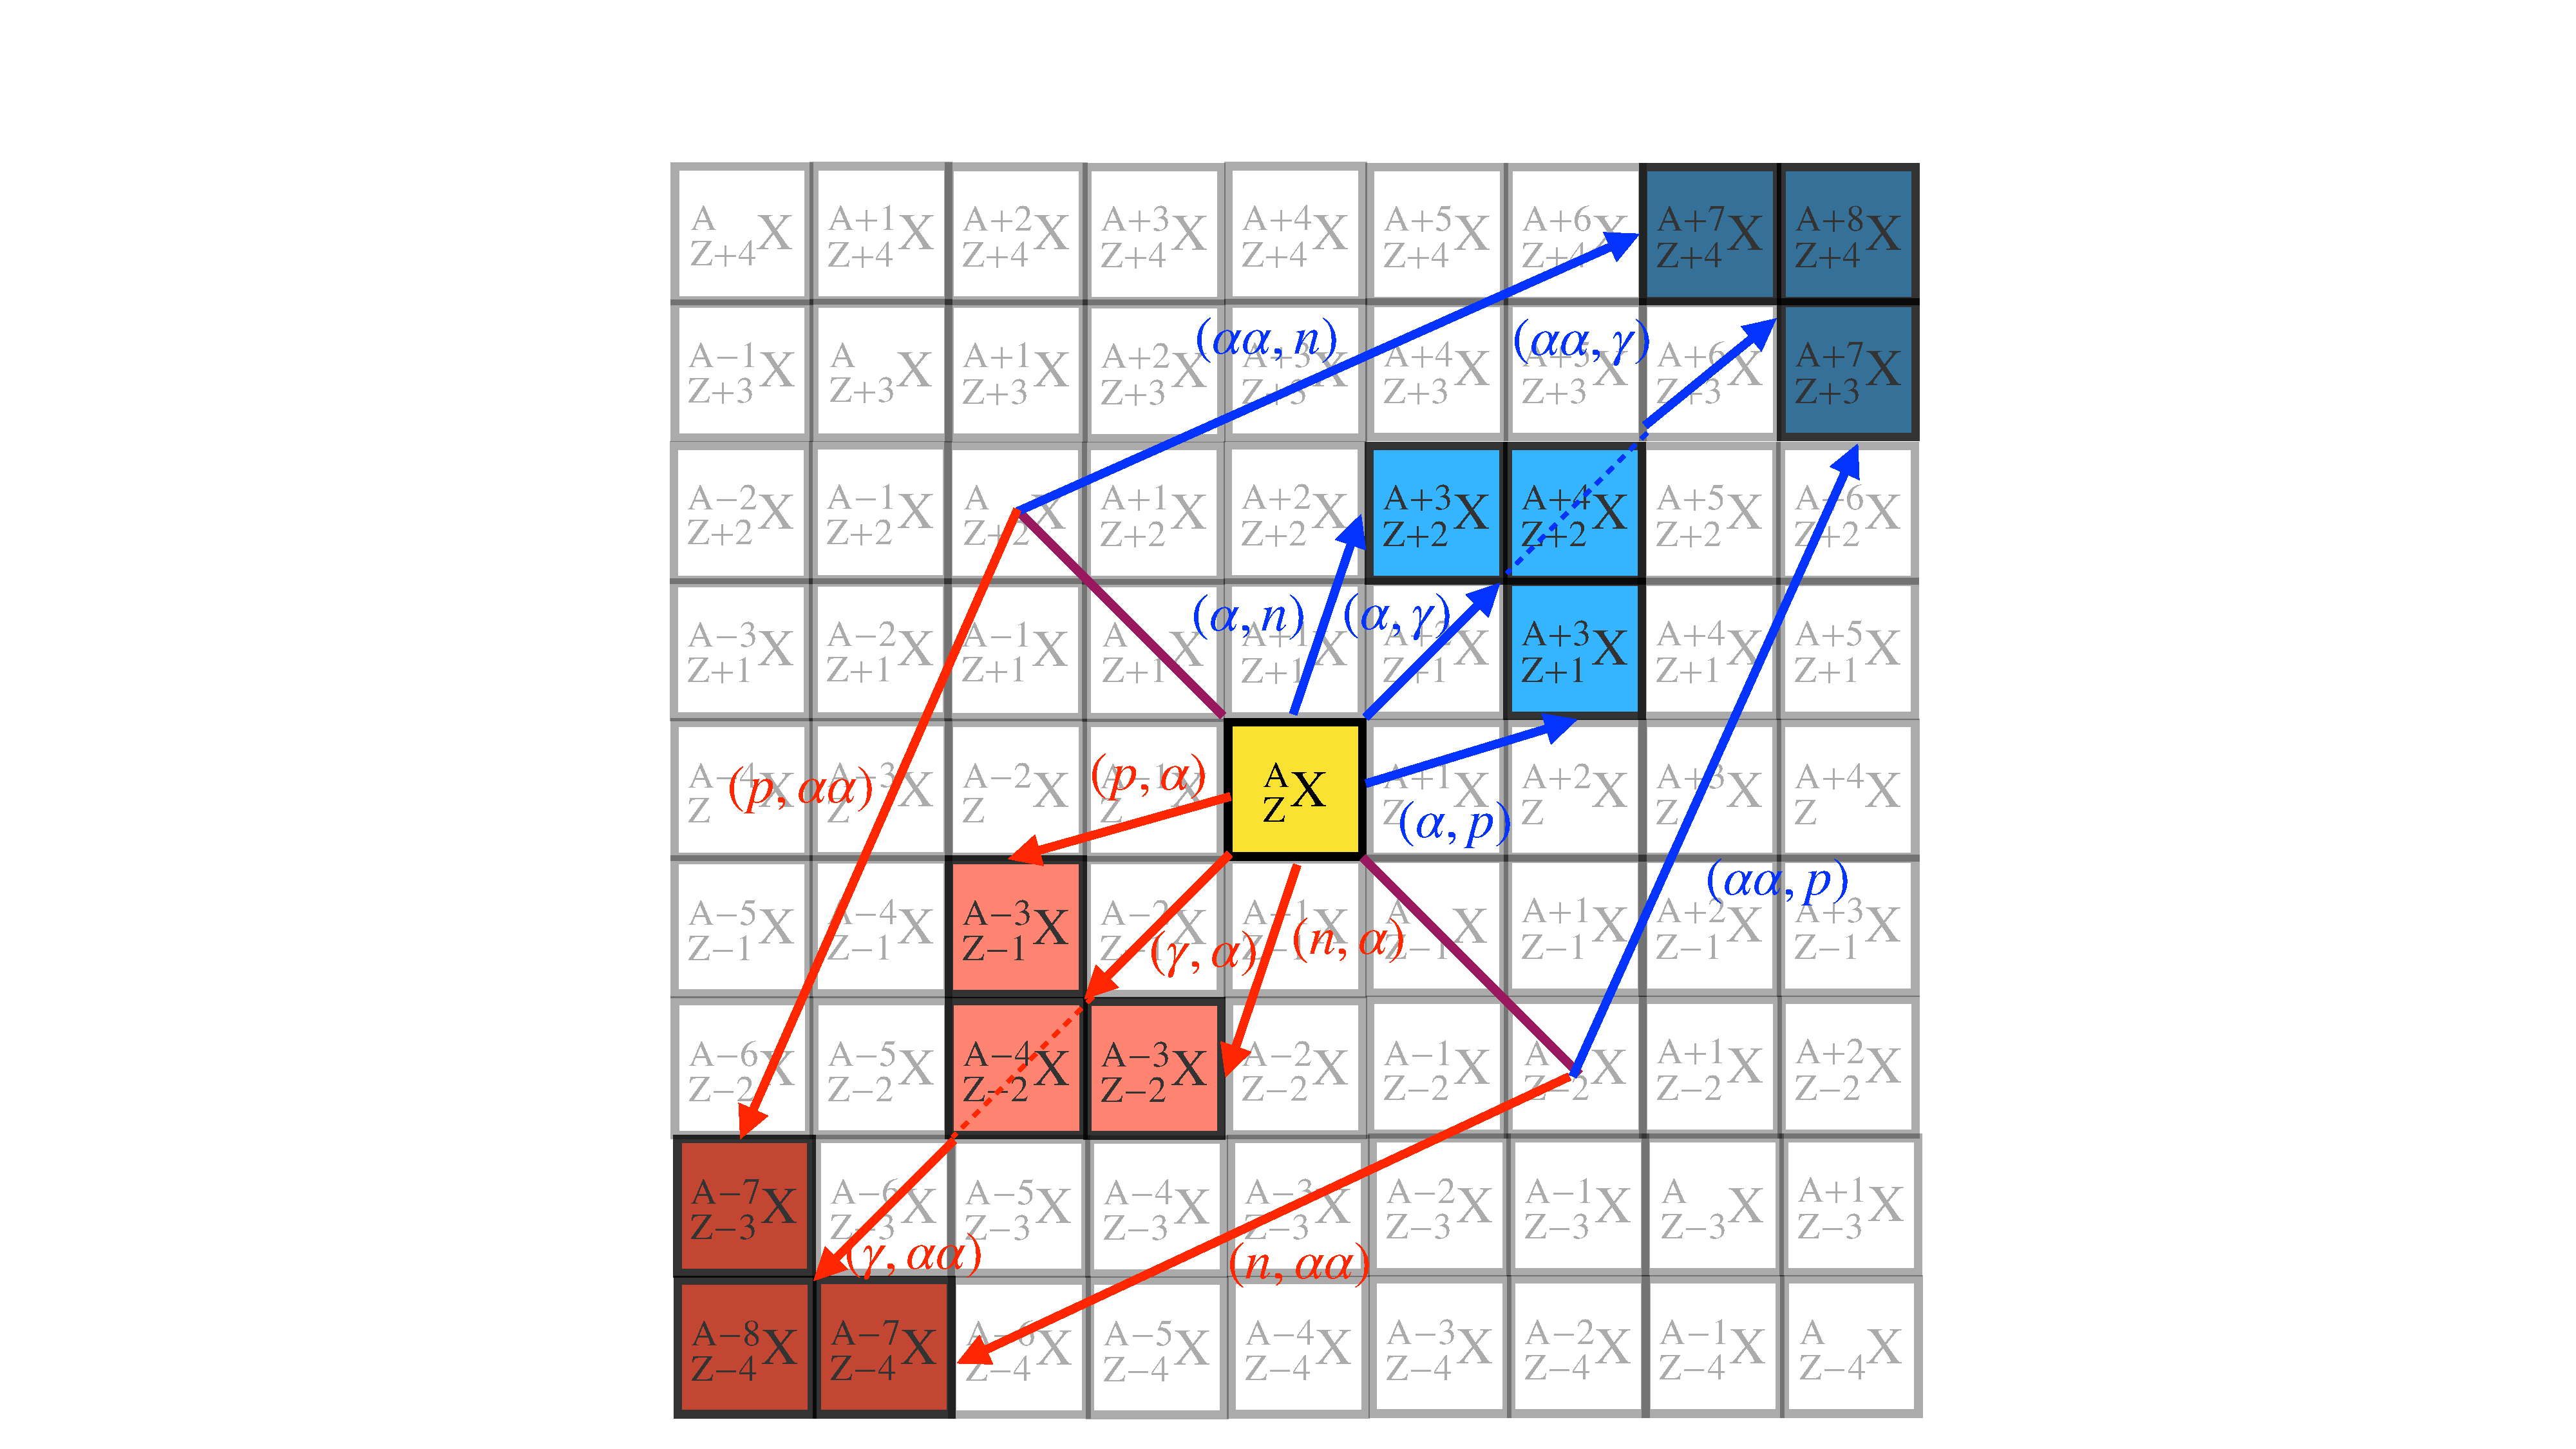
\includegraphics[scale=0.25]{Graphs/alphaChart.pdf}
	\caption[Alpha reactions chart]{Alpha reactions chart. }
	\label{fig:alphaChart}
\end{figure}

Additionally, as the mass number of nuclei growths, cluster decay becomes feasible given the increasing instability of the very heavy. Examples of cluster nuclei such as  $\mathrm{{}^{23}F}$, $\mathrm{{}^{22,24,26}Ne}$, $\mathrm{{}^{28,30}Mg}$, $\mathrm{{}^{32}Si}$, $\mathrm{{}^{38,42}S}$ and $\mathrm{{}^{46}Ar}$ appear to be relevant in the context of superheavy nuclear decay \cite{maroufi_dehghani_alavi_2019}. \\


\subsection{The s and r processes} \label{sub:srProcesses}

Heavy nuclei neutron capture occurs with the relative slow paced s-process, and the more rapid r-process. This difference in the rate of these processes is correlated with the characteristics of the astrophysical environments in where they are involved. While the former are typical in the case of nuclei production within the valley of stability in asymptotic giant branch stars, the latter occurs in extremely high neutron density scenarios associated with certain kind of supernovae, X-ray events or white dwarf to neutron star mergers. \\

The s-process involves neutron capture periods are comparable to the competing $\beta$ decay reaction.  The main sequence to produce the s-process is given by: 

\begin{equation}\label{eq:reaction_sprocess_source}
	\mathrm{{}^{14}N(\alpha, \gamma) {}^{18}F(\beta^+, \nu) {}^{18}O(\alpha, \gamma) {}^{22}Ne(\alpha, n) {}^{25}Mg}.
\end{equation}

This process contributes to explain nuclei diversity with $A > 60$ \cite{kappeler_2005} and it stops when the most stable heavy nucleus $\mathrm{{}^{209}Bi}$ is reached \cite{iliadis_2015}. Additionally, $\mathrm{{}^{13}C(\alpha, n){}^{16}O}$ also contributes to neutron production. However, the responsible for the $\mathrm{{}^{13}C}$ pocket is not entirely well understood s-process known and unknown \cite{lattanzio_lugaro_2005}. \\

Beyond $\mathrm{{}^{209}Bi}$, the s-process is truncated.  Further neutron rich nucleosynthesis with $A>209$ is exclusively explained by the r-process \cite{qian_vogel_wasserburg_1999}. However, the later also produces neutron rich nuclei below the bismuth threshold and therefore it coexists with the s-process. Nonetheless, r-process reactions are more favored at explosive environments related to core collapse to neutron star mergers. For example, explosive environments take place within 8-10 $M_{\odot}$ with a network involving about 3600 different processes \cite{wanajo_tamamura_itoh_nomoto_ishimaru_beers_nozawa_2003}. \\

Additionally, the radiative capture of neutrons $(n, \gamma)$ are fueled by the $(p, n)$ and $(\alpha, n)$ source reactions. The standard production takes place with nuclei with $A \sim 66$ and if enough neutrons are produced, the $\alpha$-particle freeze out, which a phenomenon that inhibits long neutron capture chains, is overcome and nuclei reach the limit of $A \sim 100$ \cite{woosley_hoffman_1992}. \\

After the freeze out, the limit for these chains is fixed by the neutron dripline. Nuclei with masses beyond that boundary are extremely unstable such that any neutron absorption will cause they to decay. When the chain touches the drip line, nuclei generally start $\beta$ decay by following specific isotones with a fixed magic number of neutrons $N = 126$ and proton number ranging $Z=64-78$ \cite{suzuki_shibagaki_yoshida_kajino_otsuka_2018}. \\

One example of a astrophysical context which allows r-process is given by explosive high entropy core collapse environments. High and rapid neutron flux is ejected and the density is given by: 

\begin{equation}\label{eq:reaction_density}
	\rho(t) = \rho_1 \exp \left( - \frac{t}{\tau}\right) + \rho_2 \left( \frac{\Delta}{\Delta + t}\right)^2.
\end{equation}

The first term is rapidly decaying and the second is parametrized with the $\Delta$ variable. Further details on this model are given in \cite{meyer_2002}. \\

Additionally, antineutrino capture assumes a role in the r-process given that they enhance neutron production by the reaction:

\begin{equation}\label{eq:reaction_antineutrino_hatne}
	\bar {\nu}_{e} + p \rightarrow n + e^{+}.
\end{equation}

In fact, given the energy and luminosity dominance of antineutrinos over neutrinos, which are associated with the competing reaction 

\begin{equation}\label{eq:reaction_antineutrino_ne}
	\nu_e + n \rightarrow p + e^{-},
\end{equation}

implies that neutrino wind, which is produced in environments like high entropy core collapse, boosts additional neutron production \cite{meyer_mclaughlin_fuller_1998}. However, electron capture does not play a noticeable role in r-process nucleosynthesis \cite{langanke_martinez-pinedo_zegers_2021}. \\

\subsection{The p and rp processes} \label{sub:pProcesses}

These proton capture processes work similarly than their corresponding neutron capture analogous given that p and rp are the slow and high paced processes respectively. The main objective of these reactions is to explain the neutron deficient nuclei. In particular, among the huge network of about  20 000 cross sections involved in p-process nucleosynthesis, only 35 neutron-deficient stable nuclei, which are named as p-nuclei, are present \cite{harissopulos_lagoyannis_spyrou_zarkadas_galanopoulos_perdikakis_becker_rolfs_strieder_kunz_et_2005}. \\

In addition to proton capture, photodisintegration occurs in three main processes with the form $(\gamma, n)$, $(\gamma, p)$ and $(\gamma, \alpha)$ during the p-process.  This process is partially fueled by the reaction $(\alpha, \gamma)$ which is involved in a competence with the neutron source $(\alpha, n)$ alternative channel. Then, certain combinations of the previous reactions permit $\mathrm{{}^{74}Se}$ and $\mathrm{{}^{78}Kr}$, the first and second of the lightest p-nuclei, to be produced. An example of a reaction chain associated with the former given by \cite{quinn_spyrou_simon_battaglia_couder_deyoung_dombos_fang_gosrres_kontos_et_2013}: 

\begin{equation}\label{eq:reactions_74Se_pProcess}
	\mathrm{{}^{74}Ge(p, \gamma){}^{75}As(p, n){}^{75}Se(\gamma, n){}^{74}Se}.
\end{equation}

Other p-nuclei are $\mathrm{{}^{92, 94}Mo}$, $\mathrm{{}^{96, 98}Ru}$, $\mathrm{{}^{138}La}$,  $\mathrm{{}^{180}Ta^{m}}$ \cite{delaeter_2008}. One distinguishable aspect is that they have recent, but not entirely certain, abundance calculations.  Additionally, alpha induced reactions are relevant in the production of further stable p-nuclei, which include $\mathrm{{}^{154}Sm}$,  $\mathrm{{}^{162}Dy}$, $\mathrm{{}^{166}Er}$ and $\mathrm{{}^{197}Au}$ \cite{le_duy_hung_2021}. \\

Ideal astrophysical scenarios are accretion neutron stars, in where reaction networks with elements up to $\mathrm{Xe}$ are expected to be formed. These heavy nuclei are reached because of the $\alpha p$ process, which consists of reactions $(\alpha, p)$ and $(p, \gamma)$ alternating to keep  heavier nuclei production. However, a first end point for the p-process in encountered $Z \le 54$ due to the existence of the $\mathrm{SnSbTe}$ cycle, which constraints the reaction chain to the production of $\mathrm{{}^{106}Te}$, $\mathrm{{}^{107}Te}$ and $\mathrm{{}^{108}Te}$ \cite{schatz_aprahamian_barnard_bildsten_cumming_ouellette_rauscher_thielemann_wiescher_2001}. In particular, instead of capturing more protons, an alpha decay truncates the chain. \\

Then, in the context of higher $A$, the more rapid and explosive rp process takes place. Some nuclei which react as $(\alpha, \gamma)$ are $\mathrm{{}^{72}Ge}$, $\mathrm{{}^{91,92}Ge}$, $\mathrm{{}^{92}Mo}$, $\mathrm{{}^{104}Pd}$, $\mathrm{{}^{116,118}Sn}$ whereas $(p, \gamma)$ reactions are found on $\mathrm{{}^{104,105,106}Pd}$ and  $\mathrm{{}^{96}Mo}$ nuclei \cite{harissopulos_spyrou_lagoyannis_zarkadas_becker_rolfs_strieder_hammer_dewald_zell_et_2005}. In fact, production of p-nuclei with $140 \le A \le 200$ is considerable sensible to $(\gamma, \alpha)$ disintegration \cite{kiss_szucs_gyurky_fulop_farkas_kertesz_somorjai_laubenstein_frohlich_rauscher_et_2011}. Eventually, the stopping point of this chain is given by the proton drip line. This drip-line is extended by a chain of Ge, As, Se, Br, Kr, Sr isotopes with $Z > N$ \cite{cai_chen_yuan_jian-jun_2022}.  When this boundary is reached, nuclear repulsion is considerable enough to inhibit additional proton capture. Then, nuclei approach the stability valley by $\beta^{+}$ decaying at special stopping points which coincide with magic number values. \\

Although abundance enhancement is predicted for selected magic numbered nuclei, masses of proton-rich above $A =60$ have been not measured entirely. The rp-process in key for high temperature burning and in neutron stars with respect X-ray emission phenomena. Masses are critical when establishing the capture-photodisintegration equilibrium point. Examples of such nuclei with a required higher precision mass measurements range from $\mathrm{{}^{61}Ga}$ to $\mathrm{{}^{73}Kr}$. Additionally, some neutron deficient nuclei are also candidates for diproton emission are  $\mathrm{{}^{64}Zn}$,  $\mathrm{{}^{59}Ge}$, $\mathrm{{}^{63}Se}$, $\mathrm{{}^{67}Kr}$, $\mathrm{{}^{71}Sr}$ \cite{brown_clement_schatz_volya_richter_2002}, which may prevent further proton accumulation to occur.

\section{Active research topics} \label{sec:activeResearch}

Some active research topics in the nuclear astrophysics field are generally introduced. A special emphasize is given to discrepancies in Big Bang nucleosynthesis abundances estimations. Additionally, challenges associated to core collapse are described from both the nuclear reaction and stellar perspectives. Finally, a short list of selected topics including core neutron star physics, very heavy nuclei and neutrino reaction are also presented. \\

Although Big Bang nucleosynthesis theory explains, to a great extent, the average composition of most of the light elements in the Universe, particularly $\mathrm{{}^{1}H}$ to   $\mathrm{{}^{4}He}$, it does not completely account for the abundance of heavier elements. $\mathrm{{}^{7}Li}$ is one of such cases where the nuclear astrophysics prediction differs from its experimental value since the $\mathrm{{}^{7}Li/H} \sim 10^{-10}$ abundance is about a factor of 3 lower than theoretically expected. A solution to this discrepancy can be achieved by replacing the classical Boltzmann with the alternative Tsallis statistics. The former is parametrized with a factor $q$, which is related to the departure from the latter. Values for the lithium problem are ranging $1.069<q<1.082$  \cite{bertulani_2019}. \\ 

Additionally, core collapse is a phenomenon that, although widely present in many nuclear astrophysics applications, is not entirely explained by current astrophysical models. Thus,  theoretical predictions of the abundances of middle and heavy nuclei are still uncertain \cite{arcones_bardayan_beers_bernstein_blackmon_messer_brown_brown_brune_champagne_et_2017}. In fact, the complexity of core collapse involves modeling the last instances in the lifetime of a star which in general comprehends challenges associated with inherent aspects of nuclear reactions, as well as it requires consistent stellar models. \\

With respect to the nuclear reactions part, low-energy experimental data of key reactions is usually absent since most experiments are performed within a higher energy window than the values of actual astrophysical interest. Then, despite increasing theoretical and instrumentation efforts, low-energy extrapolations of cross sections and S-factors are still considerably uncertain to accurately predict many middle heavy nuclei abundances \cite{carlson_carpenter_casten_elster_fallon_gade_gross_hagen_hayes_higinbotham_et_2017}. Current experiments in detection of heavy nuclei are essential to determine the distribution of elements, specially in events like the fusion of neutron stars. \\ 


On the other hand, from stellar modeling perspective, star collapse understanding is sensible to changes in initial conditions of stars which are classified depending on the kind and age of the star with respect to the Universe. Additionally, core collapse modeling is as well challenged by the accuracy of current knowledge of explosive environments like supernovae with mechanisms not completely well explained \cite{bertulani_kajino_2016}, like is the case of the Ia type supernova. This uncertainty is also present when studying neutron star mergers, which is a topic of recent active research due to the potential production of super heavy nuclei with $A > 100$ at these environments.  \\

A closely related topic to core collapse is the study of the core of a neutron star, which is believed to have the conditions to host new exotic states of matter characterized by extreme highly density and degeneracy. A new state of matter, which is called the quark-gluon plasma, has been proposed to be present in such extreme scenarios. Particularly, the pressure $p$ generated  by a degenerate object is given by \cite{kundt_2005}: 

\begin{equation}\label{eq:reaction_degenerate}
	p \sim \rho^{\gamma},
\end{equation} 

where $\rho$ is the density and $\gamma$ a coefficient associated with the equation of state. This state could simulate conditions on the primordial Universe when quarks were not bounded in structures like protons or neutrons \cite{bertulani_kajino_2016}. Additionally, its study could shed light on black hole formation mechanisms and could explain how matter is affected during that process. \\

Under extreme nucleosynthesis scenarios, heavy and superheavy nuclei production is widely known to take place. However, clarifying their synthesis mechanisms is essential to explain the physics underling very unstable nuclei formation, which might be critical in understanding highly explosive processes mediated by rapids r and rp processes. For example, heavy nuclei reactions like the $Z = 119, 120$ fusion with form $\mathrm{{}^{26}Mg + {}^{248}Cm \rightarrow {}^{274-xn}Hn +xn}$ have been studied. The $x$ is a convention for a number ranging from 3 to 5. The proposed main fusion mechanism is explained by a three-step process with steps: quasifission, when nuclei are held together, symmetrization, which occurs when clusters are exchanged, and complete fusion, when the remaining unified nucleus is completed \cite{adamian_antonenko_2022}. \\

Another example of very high nuclei involves isotopes of $\mathrm{Hs}$, $\mathrm{Mt}$, $\mathrm{Ds}$ and $\mathrm{Rg}$ with relative light targets constrained by $Z = 6-18$. If they react, currently unobserved isotopes like $\mathrm{{}^{285}Cn}$, $\mathrm{{}^{294, 295}Lv}$, $\mathrm{{}^{295, 296}Lv}$ and $\mathrm{{}^{295-298}Og}$, which extend the stability island boundaries, are expected to be produced. More detailed information on these processes is given in \cite{adamian_antonenko_2022}.  \\


Another topic related to special reactions is neutrino nucleosynthesis. Although neutrinos are present in several classical reactions, they are nucleosynthesis catalysts of core collapse given the amount of energy they have. They can trigger neutrons and protons production and then affect the rates of s, r, p and rp processes.  A relevant chain of neutrino and anti-neutrino pair begins with an electron capture

\begin{equation}\label{eq:reaction_neutrino}
	X + e^{-}\rightarrow X' + \nu 
\end{equation}

and ends by returning to the initial $X$ nucleus via the $\beta$ decay process: 

\begin{equation}\label{eq:reaction_neutrino_2}
	X' \rightarrow X + e^{-} + \bar \nu.
\end{equation}

Still, neutrinos are challenging to model theoretically to the extent that their study is an unsolved issue motivates extensions of the standard model of particle physics. For example, some of them oscillate due to quantum-mechanical effects. Additionally, alternative channels are associated with  two neutrino double beta decay with the from

\begin{equation}\label{eq:reaction_neutrino_doubleBeta}
	X \rightarrow X' + 2e^{-} + 2\bar \nu.
\end{equation}

This is a frontier topic as it is involved in decays of several nuclei ranging form Ca to Te, which affect heavy nuclei production. More information about cutting edge neutrino nucleosynthesis is given in \cite{bertulani_kajino_2016}. \\

\chapter{Astrophysical S-factor models} \label{ch:sfactorModels}

There are several methods for estimating the astrophysical S-factor. Each method is more convenient depending on the nature of the reaction. For example, method accuracy can vary depending on  the reaction type or the existence of resonant phenomena. Additionally, the methods are based on a specific approach when modeling the S-factors. In this section, the principal methods of estimating the astrophysical S-factors will be reviewed.

\section{Microscopic models} \label{sec:microscopicalModels}

Microscopic models use nuclear substructures and their interactions to provide a low level quantum mechanical description of nuclei. An initial example of such approach is given by the interaction picture of the Hamiltonian $H$ is given by: 

\begin{equation} \label{eq:micro_hamiltonian}
	H = \sum_{k} T_k + \sum_{k} V_k (r) + \sum_{k \neq j} V_{kj}(r),
\end{equation}

where $T_k$ corresponds to the kinetic energy term of the $k$th nucleon. Similarly, $V_k(r)$ is the onsite contribution related with field potential, which is felt by every nucleon, and the terms $V_{kj}$ corresponds to a two nucleon interaction across nucleons labeled as $k$ and $j$. \\

In order to find the Hamiltonian, a concrete form of a potential is then introduced. For example, the shape of a $NN$ (nucleon) potential, is included to model nucleon to nucleon interactions. Additionally, a surprising feature of the nuclear force is that a three nucleon interaction is also possible. At the fundamental level, quantum chromodynamics predicts the gluing of quarks by themselves and complex couplings. An example of a Hamiltonian with such interaction included is:

\begin{equation} \label{eq:micro_hamiltonian_NNN}
	H = \sum_{k} T_k + \sum_{k} V_k (r) + \sum_{k \neq j} V_{kj}(r) +   \sum_{k, j ,l } {V_{k, j, l}}.
\end{equation}

This direct approach is preferred in the context of light nuclei modeling. However, in the case of heavier nuclei, this approach in usually no longer feasible since nuclear interactions are complex to model individually even for few nucleons. Actually, it is challenging to compute nucleon wave functions individually and then to make reliable predictions on the physics of the entire heavy nuclei. Instead, several techniques are used to simplify the picture offered by this many nucleons and their interactions microscopical formalism. \\

One of such ideas consists of modeling the nucleus as a consequence of collective behavior. This approach is closely related to extending the Fermi nuclear model and it pretends to model the nucleus as a whole system. Examples are provided by modeling the nucleus as waves (random phase approximation) or as a fermionic molecule (antisymmetric fermionics molecular dynamics).  \\

Other proposal is to consider that the nucleus consists of various shells occupied by their nucleons. This is closely related to the nuclear shell model presented in section \ref{ssub:nuclearShellModel} with more sophisticated interactions and components to be considered. Some models leans to consider a number of cores with some valence nucleons (N-core shell model), while others (no core shell model ) aim to explain the nucleus without a central core. Pairing is included by considering the couplings within nucleons on their shells.  \\

A related technique to shell modeling is mean field potential. The general idea of this approach is that all the nucleons generate a collective potential, which is felt by all the nucleons. Wave functions are estimated by a guessing process. This is related with the Hartee-Fock formalism applied to nuclear physics. Alternatively, density functional theory is also included within this framework. Additionally, as it happens with shell models, pairing is included via interactions between components. \\

An alternative approach is to consider the nucleus to be a wrapper of minor nuclei. Then, this approach extends nucleon to cluster interactions, which considerably reduces the complexity of the computations. In order to achieve this result, a potential is introduced for interactions of clusters, for instance the $\alpha-\alpha$ potential. Then, the nuclear physics of the nucleus is described as the composite effect of the interactions of its contained clusters. \\

Finally, not all the models can be uniquely identified with one of the previous approaches. In contrast, they might combine various advantageous aspects of the previous approaches in order to improve nuclear modeling.\\

\subsection{\textit{Ab initio} models} \label{sub:microscopical_abinitio}

These models start from first principles without prior empirical or phenomenological assumptions. 
On the other hand, clusters consider the system of interacting nuclei as a whole. In particular, there are models based on \textit{ab initio} assumptions about a particular set of nuclei.  \\
 

\subsubsection{No core shell model} \label{ssub:abInitio_NCSM}

This model starts with a general picture for the Hamiltonian of all nucleons, which is expressed as \cite{barrett_navratil_vary_2013}: 

\begin{equation}\label{eq:micro_NCSM_hamiltonian}
	H = \frac{1}{A} \sum_{a < b} \frac{(\hat p_a - \hat p_b)^2}{2m} + \sum_{a<b} V_{\mathrm{NN}, ab} +  \sum_{a<b < c} V_{\mathrm{NNN}, abc},
\end{equation}

where $a, b, c$ are indexes conveniently chosen to consider all the possible $NN$ and $NNN$ interacting nucleons without repetition. Their respective potentials are $V_{\mathrm{NN}, ab}$ and  $V_{\mathrm{NNN}, abc}$.  Additionally, the first term corresponds to the relative kinetic energy. \\

One convenient expression for the potential energy, as seen by the center of mass, is given in close analogy with the harmonic oscillator. Particularly, that potential, which is labeled as $U_{\mathrm{CM}}$, is given by:

\begin{equation}\label{eq:micro_NCSM_potentialHarmonic}
	U_{\mathrm{CM}} = \frac{1}{2} A m \Omega^2 \vec {R}^2,
\end{equation}

with $\Omega$ being the frequency of the harmonic oscillator basis, $A$ the total number  and $m$ corresponds to the mass of nucleons. Additionally, $\vec {R}^2$ has the form: 

\begin{equation}\label{eq:micro_NCSM_R}
	\vec R = \frac{1}{A}\sum_{}^{A} \vec r_k, 
\end{equation}

where $\vec r_k$ is the position of the $k$th nucleon. \\

In order to solve a system with this approach, there is a special basis to be formed in terms of combinations of the positions. Thus, a generalization on the usual coordinates is needed, which is a term closely related to the Jacobi coordinates. For instance, the first Jacobi coordinates vector is given by: 

\begin{equation}\label{eq:micro_NCSM_jacobi0}
	\vec \xi_0 = \sqrt{A} \vec R.
\end{equation}

Also, if the interest is to measure the difference between the first two nucleon systems, the second Jacobi coordinate is better to be used. It has the expression: 

\begin{equation}\label{eq:micro_NCSM_jacobi1}
	\vec \xi_1 = \sqrt{\frac{1}{2}} (\vec r_1 - \vec r_2).
\end{equation}

Later, the third coefficient, which is estimated with tools of the previous coefficients, is given by: 

\begin{equation}\label{eq:micro_NCSM_jacobi2}
	\vec \xi_1 = \sqrt{\frac{2}{3}} ( \frac{1}{2}(\vec r_1 - \vec r_2) - \vec r_3).
\end{equation}

If the iteration continues, a generalized coefficient of order $A - 1$ is given by: 

\begin{equation}\label{eq:micro_NCSM_jacobiA-1}
	\vec \xi_{A-1} = \sqrt{\frac{A-1}{A}} \left( \frac{1}{A-1}(\vec r_1 +  \vec r_2 + ... + \vec r_{A - 1}) - \vec r_A  \right).
\end{equation}

This approach considers that the nuclear phenomena are explained by taking into account the nucleons of the outer or valence shell and the pairing of the outer nucleons. Then, it is said that the model does not recognize an actual core, so that it is called no core shell model \cite{barrett_navratil_vary_2013}. \\


NCSM gives an alternative of other shell models since its modeling strategy is centered in proposing nuclear collective behavior \cite{freer_horiuchi_kanada-enyo_lee_meisner_2018}. The Hamiltonian for the nucleon $k$ on this formalism is given by: 

\begin{equation}\label{eq:micro_NCSM_Hamiltonian}
	H_k = -\frac{\hbar^2}{2m} \nabla^2_k + \frac{1}{2} m \Omega^2 r^2_k,
\end{equation}

where $\Omega$ corresponds to the angular frequency of collective nuclear vibrations. \\

Additionally, there are alternatives to express the NCSM formalism by considering a symmetric operator based approach. This is given in terms of the creation $c^{\dagger}$ and annihilation $c$ operators. Then, the Hamiltonian is expressed as $H_k$ is expressed as: 

\begin{equation}\label{eq:micro_NCSM_symmetric_Hamiltonian}
	H_k = \hbar \Omega \left (c^{\dagger}_{x, k} c_{x, k} + c^{\dagger}_{y, k} c_{y, k} +  c^{\dagger}_{z, k} c_{z, k} +  \frac{3}{2}  \right).
\end{equation}

The last term of the previous equation shows a base term  $3\hbar\Omega/2$ which is expected ground state energy of a three dimensional harmonic oscillator. \\

An application to nuclear reaction for a collision within this framework is given by a description of the initial nucleus $A - a$, which is the target, which collides with the projectile $a$. In all cases, isospin, parity and angular momenta are considered. A basis function of the composite state of the system is given by \cite{barrett_navratil_vary_2013}:

\begin{equation}\label{eq:micro_noCoreShell_basis}
	| \Phi^{J^{\pi} T}_{\nu r} \rangle  = \left [ |A -a \alpha_1 I^{\pi_1}_1 T_1 \rangle | a \alpha_2  I^{\pi_2} T_2 \rangle  Y_l (\Delta \hat r)\right] \frac{\delta(r - |\Delta \vec r|)}{r  |\Delta \vec r|}, 
\end{equation}

where $\nu$ corresponds to a collection of uniquely identifying quantum numbers, $\pi_1$ and $\pi_2$ are associated with the parties of the reactants. Similarly, the pair $T_1$ and $T_2$ is related with the isospins, and $\alpha_1$ and $\alpha_2$ are indicators of the energy state of the reactants and  $\Delta \vec r$ corresponds to the separation vector between clusters with mass numbers $A - a$ and $a$.\\

Then, when continuum is incorporated, the expression for the wave function takes $\Psi$ the form \cite{dohet-eraly_navratil_quaglioni_horiuchi_hupin_raimondi_2016}:  \\

\begin{equation}\label{eq:micro_noCoreShell_continuum}
	| \Psi^{J^{\pi} T} \rangle  = \sum_{\lambda} c_\lambda | \lambda J^{\pi} T \rangle  + \sum_{\nu} { \int {r^2 \frac{\gamma_\nu(r)}{r} \hat {\mathcal{A} }  | \Phi^{J^{\pi} T}_{\nu r} \rangle dr} },
\end{equation}

where $T$ is the isospin, $\nu$ is a set of selected quantum numbers, $\gamma_\nu$ is the continuous amplitude and $c_\lambda$ is the coefficient for the discrete amplitude. Additionally, $\mathcal{A}$ assumes the role of an antisymmetrization operator, which is defined as \cite{freer_horiuchi_kanada-enyo_lee_meisner_2018}: 

\begin{equation}\label{eq:micro_noCoreShell_antisymmetrization}
	\mathcal{A} = \frac{(A - a)! a!}{A!}  \sum_{P} \mathrm{sgn} (P) P,
\end{equation}

where $P$ represents each of the possible permutation and $\mathrm{sgn}(P)$ accounts for the sign of the permutation. \\ 

Finally, an example of NCSM applied to the study of  $\mathrm{{}^{7}Be}$,  $\mathrm{{}^{8}B}$ nuclei is provided by the \textit{ab initio} approximation made by  \cite{navratil_bertulani_caurier_2006}. One of the free parameters of the model is $\Omega$, which permits the definition of energies of the form $N\hbar \Omega$, where $N$ is an integer, to parametrize the numerical solution of the system. Particularly, the spectroscopic factor $S$, which is a measure of the incidence of microscopical phenomena in the cross section, can be estimated by: 

\begin{equation}\label{eq:micro_NCSH_application_S}
	S = \int { \left| g (r) \right|^2 r^2 dr },
\end{equation}

where $g(r)$ corresponds to a form factor of the channel cluster characterized with $A - 1$, with $A$ being the mass number, $I_1$ for the isospin, $l$ for the orbital and $J$ for the angular momentum and $r$ is associated with the norm of the vector: 

\begin{equation}\label{eq:micro_NCSH_application_r}
	\vec r  = \frac{1} {A - 1}( \vec r_1 + \vec r_2 + ... + \vec r_{A-1}) - \vec r_A,
\end{equation}

where $\vec r$ has the role of the relative difference between the position of the last nucleon $\vec r_A$ with respect to the average of the rest. This parameter is useful when parametrizing the radial components of the wave function. \\

One of the properties of the form factor is its asymptotic behavior, which is closely related with the Coulomb wavefunctions. The particular expression is given by: 

\begin{equation}\label{eq:micro_NCSH_application_asymptotics}
	r g_{lj}(r) \rightarrow C_{lj} W_{-\eta , l + 1/2} (2k_0r), 
\end{equation}

where $k_0 = \sqrt{2\mu E_0/\hbar^2}$ with $E_0$ the nucleon separation energy. Additionally, $W$ corresponds to the Whittaker function evaluated with the parameters $\eta$ for the Sommerfeld parameter and $l$ for the relative angular momentum. In order to complete the picture, the asymptotpic normalization coefficient $C_{lj}$ is added.  \\


\subsubsection{Electroweak reaction models} \label{ssub:micro_abinitio_electroweak}

Electroweak phenomena like beta decay can be studied with the no core shell model framework \cite{atkinson_navratil_hupin_kravvaris_quaglioni_2022}. In particular, a cluster expansion may be introduced in order to facilitate computations. The relevant variables are the angular momentum parity pair $J^\pi$, the isospin $T$. The operator, which is referred as the Gamow-Teller, is defined as: 

\begin{equation}\label{eq:micro_NCSM_beta_asymptotics}
	B = \frac{1}{2} \langle \Psi || \mathcal{GT} || \Psi ' \rangle, 
\end{equation}

where $\Psi$ and $\Psi'$ are the incident and outgoing wave functions respectively. Additionally, the Gamow-Teller operator is given by: 

\begin{equation}\label{eq:micro_NCSM_beta_GToperator}
	\mathcal{GT} = \sum_{k = 1}^{A} \hat \sigma_k \hat \tau_k^{\tau},
\end{equation}

where $\hat \sigma_k$ corresponds to the operators associated with the Pauli matrices and $\hat \tau_k$ are the isospin raising operators, which is similar to $L^{+}$ in quantum mechanics. Additionally, $A$ corresponds to the mass number. \\ 

Further computations regarding to equation \ref{eq:micro_NCSM_beta_asymptotics} are performed on top of expanding the transition matrix coefficient: 

\begin{equation}\label{eq:micro_NCSM_beta_transition}
	\langle \Psi | \hat O |  \Psi ' \rangle,
\end{equation}

where $\hat O$ corresponds to a suitable operator for one body. The computations now proceed with a similar path to what was described in the ansatz of equation \ref{eq:micro_noCoreShell_continuum}. \\

A key of the predictions of this model is half live $T_{1/2}$ for the $1/2^{+}$ state. The general phenomenological expression gives a proportionality relation of: 

\begin{equation}\label{eq:micro_NCSH_beta_halflive}
	T_{1/2} \propto \frac{1}{g^2_A B},
\end{equation}

where $g_A$ corresponds to the coupling constant associated with the Gamow-Teller interaction.\\

Alternatively, modern theories \textit{ab initio} electroweak reactions use correlated a variational version of the stochastic  Monte Carlo method to make accurate predictions \cite{marcucci_nollett_schiavilla_wiringa_2006}. Special NN  potentials are used to achieve this objective. For example, one of such potentials, the AV18, has the form: 

\begin{equation}\label{eq:micro_modernTheories_AV18_NN}
	v_{ab} = \sum_{p} v_p(r_{ab}) O^{p}_{ab},
\end{equation}

where the index $p$ accounts for the components and the operator $O$ is defined as:

\begin{equation}\label{eq:micro_modernTheories_AV18_O}
	O^{p}_{ab} = [1, \vec \sigma_a, \vec \sigma_b, S_{ab}, \vec L \cdot \vec S ] \otimes [1, \vec \tau_a \cdot \vec \tau b],
\end{equation}

where $1$ is the identity operator, $\vec \sigma_a \cdot \vec \sigma_b$ corresponds to the dot product of the Pauli matrices with labels $a$ and $b$. Similarly, $\vec L \cdot \vec S$ denotes the product of the relative orbital angular momentum and spin operators respectively. Additionally, $\vec \tau_a \cdot \vec \tau_b$ represent the product of the Pauli matrices for isospin.  \\

In the specific case of weak processes, the total cross section is given by:

\begin{equation}\label{eq:micro_modernTheories_weak_crossSection}
	\sigma^{(\beta)} (E) = \int {2\pi \delta (E_0 - E_f) \frac{1}{v} 	{g \frac{d\vec p_e}{(2\pi)^3} \frac{d\vec p_\nu}{(2\pi)^3} }  },
\end{equation}

with $\vec v_e$ and the integration variables $\vec v_\nu$ label electron and neutrino momentum.   In addition, $E_0$ and $E_f$ account for the initial and final energies. The element matrix in contained within the term $g$, which is defined as:

\begin{equation}\label{eq:micro_modernTheories_weak_crossSection_g}
	g = \sum_{s_e s_\nu} \sum_{M_1 M_2} {\frac{1}{(2J_1 + 1)(2J_2 + 1)}|\langle f | H_{W} |0 \rangle|^2 },
\end{equation}

where $s_e$ and $s_\nu$ are the indexes running for electron and neutrino spin values, as well as $M_1$ with $M_2$ corresponds to the pair of projections of the angular momentum. Additionally, the label $f$ and $0$ denote final and initial states respectively and $H_W$ denotes the Hamiltonian of the weak interaction. \\

An alternative way to express $g$ is given by:

\begin{equation}\label{eq:micro_modernTheories_weak_crossSection_g_alternative}
	g = (2\pi)^2 G^{2}_V L_{\sigma \tau} N^{\sigma \tau},
\end{equation}

with $G_V$ as the Fermi constant and $L^{\sigma \tau}$ and $N^{\sigma \tau}$ as the lepton and nuclear tensors. These factors are allowed to be expressed in terms of multipole expansion. \\

From the stochastic point of view, another method is the variational Monte Carlo, which is used for estimating the bound states wave functions. The form of the trial wave function is given by:

\begin{equation}\label{eq:micro_modernTheories_variationalMonteCarlo}
	| \Psi_V \rangle = \left[ 1 + \sum_{a < b < c} U_{abc}\right]  \left[ \mathcal{S}  \prod_{a < b \le A } {(1 + U_{ab})}\right] | \Psi_J\rangle ,
\end{equation}

with $\mathcal{S}$ as the symmetrization operator and the terms of the form $U_{ab}$ are associated with the correlation operators. Additionally, $|\Psi_J\rangle$ is referred to as the Jastrow wavefunction.  These have a direct connection with the $O^{p}_{ab}$ in the frame of NN interactions, as given in equation \ref{eq:micro_modernTheories_AV18_O}. The related formula is given by:

\begin{equation}\label{eq:micro_modernTheories_variationalMonteCarlo_correlation}
	U_{ab} = \sum_{p} u_{p}(r_{ab}) O^{p}_{ab},
\end{equation}

where $u_{p}(r_{ab})$ is associated with the radial wave function evaluated at position $r_{ab}$. Meanwhile, the operators $U_{abc}$ correspond to three correlations.  \\

Depending on the case, $|\Psi_J \rangle$ assumes a different form. For the simplest case, which corresponds to a type s shell, the Jastrow wave function is given by:

\begin{equation}\label{eq:micro_modernTheories_variationalMonteCarlo_Jastrow}
	| \Psi_J \rangle  = \left[ \prod_{a < b \le A }{f^{d}_{abc}} \right] \left[ \prod_{a < b \le A }{f_d(r_{ab})} \right] |\Phi_A \rangle
\end{equation}

with $f_d(r_{ab})$ and $f^{d}_{abc}$ as the two and three body correlation functions. Additionally, the state $|\Phi_A \rangle$ is obtained from the Slater determinant of the states of the nucleons, which are determined by a convenient selection of basis functions.  \\

\subsection{Many body models}  \label{sub:microscopical_manybody}

The nucleus can be modeled as a many body system. Naturally, the nucleons are the components of this bounded system. In addition, the interactions between the components of the nucleus are nuclear interactions of a certain shape and form.  Many body models take into account the different bodies that make up the nuclei. Therefore, cross section determination is reduced to the analysis of a many body quantum mechanics problem with all the nuclear compounds. Also, nuclei deformation can be considered in models. \\

\subsubsection{Three body models}

One particularity of the nuclear interaction is that there are three body forces presents.  These contributions are considered only when three nucleons interact and are known as $NNN$ interactions  \cite{grigorenko_danilin_efros_shulgina_zhukov_1998}. The existence of this novel type of nuclear forces is partially explain by the fact that quarks, the ultimate constituencies of nucleons, have the ability of coupling with not only other quarks, but also with themselves. \\

One of the advantage of this approach is that cluster effects can be considered. A description of $NNN$ interactions applied to clusters are given in  \cite{grigorenko_danilin_efros_shulgina_zhukov_1998}. This study is centered in modeling the $\mathrm{{}^{8}Li}$ or $\mathrm{{}^{8}B}$ nuclei, a three force picture composed of: $\alpha$, $t$ and a nucleon $N$ is used.  \\

The starting point consists of assigning the wave function of the system  $\Phi$  the form:  \\

\begin{equation}\label{eq:micro_threeBody_wavefunction}
	\Phi = \Psi(X, Y) \prod \Phi_k, 
\end{equation}

where $\Phi_k$ represent the wave function of each of the $k$ clusters. Then, $\Psi(X, Y)$ can be assigned to a contribution due to the three body interaction. This interaction is parametrized by the coordinates $X$ and $Y$,  which are related with angular momentum considerations and are known as Jacobi coordinates. \\

Now, the $\Psi(X, Y)$ function can be splitted in an asymptotic two nucleon like interaction $\Psi^{(2)}$ and the actual pure three force wave function $\Psi^{(3)}$ . Then, $\Psi(X, Y)$ can be expressed as: 

\begin{equation}\label{eq:micro_threeBody_splitting}
	\Psi(X, Y) = \Psi^{(2)}(X, Y) +  \Psi^{(3)}(X, Y).
\end{equation}

The three body term can be defined in terms of hyperspherical harmonics, which are one of the approaches towards the characterization of the $NNN$ interaction. Particularly, $ \Psi^{(3)}(X, Y)$ is given by: 


\begin{equation}\label{eq:micro_threeBody_psi3}
	\Psi^{(3)}(X, Y) = \rho^{-5/2} \sum_{K, \nu}^{\mathcal{K}} {\chi_{K, \nu}(\rho) \mathcal{J}_{K, \nu} (\theta, {\hat n}_x, {\hat n}_y ) },
\end{equation}

where $\nu$ is a collection of quantum number which includes rotations from the $x$ and $y$ coordinates $l_x$ and $l_y$, the orbital angular momentum $L$ and the spins $S$, $S_x$. Also, the hyperspherical harmonic $\mathcal{J}_{K, \nu}$ depends on a rotation angle $\theta$ and unitary vectors in the $x$ and $y$ axes ${\hat n}_x$ and ${\hat n}_y$ respectively. Additionally, $\rho$ is a quantity that absorbs the dependence of $\Psi^{(3)}$  with respect to the Jacobi coordinates and can be associated as a radial distance.  Particularly, this dependence is expressed as: 

\begin{equation}\label{eq:micro_threeBody_rho}
	\rho = \sqrt{ \frac{12}{7} X^2 + \frac{7}{8} Y^2}.
\end{equation}

The index $K$ helps tag each term contributing to equation \ref{eq:micro_threeBody_psi3}, which can be interpreted as a generalize partial wave expansion with $K$ having an analogous role to $l$ in the classical three dimensional picture. In fact, $\mathcal{K}$ is the truncation value of the $K$-series. Additionally, the generalized radial-like part of the expansion corresponds to  $\chi_{K, \nu}$. Its asymptotic behavior is given as: 

\begin{equation}\label{eq:micro_threeBody_chiAsymptotics}
	\chi_{K, \nu} \rightarrow \rho^{-5/2} \exp{ (- \kappa \rho)},
\end{equation}

where $\kappa = \sqrt{2mE_{\mathrm{3-sep}}}$ has an analogous to the wave number with $m$ and $E_{\mathrm{3-sep}}$ being defined as the nucleon mass and separation energy of the three body system. \\
	
On the other hand, the two body term of the wave functions is given by the asymptotic behavior of the Coulomb terms for the subsystems tagged with $x$ and $y$. Particularly, $\Psi^{(2)}$ is expressed as: 

\begin{equation}\label{eq:micro_threeBody_psi2}
	\Psi^{(2)}(X, Y) =  \sum_{\alpha} {f_\alpha (\rho) \psi_{l_xj_x}(X) \psi_{l_yj_y}(Y) }, 
\end{equation}

where $\alpha$ is an index running through all the values of $l_x$, $l_y$, $j_x$ and $j_y$. Also, like it happens with the expression of $chi_{K, \nu}$ of equation  \ref{eq:micro_threeBody_chiAsymptotics}, the functions $\psi$ obey asymptotics. In this concrete case, the extreme behavior is given as: 

\begin{equation}\label{eq:micro_threeBody_psi2_asymptotic}
	\psi_{l_{z}j_{z}} = W_{-\eta_{z}, l_x + 1/2}(2K_{z}(Z)),
\end{equation}

where the index $z$ and $Z$ can be replaced by $x$ and $X$ in the case of $\psi_{l_{x}j_{x}}$ and, reciprocally, by $y$ and $Y$ for $\psi_{l_{y}j_{y}}$. Furthermore, $W$ corresponds to the Whittaker functions, which are closely related to the Coulomb functions, evaluated with the Sommerfeld parameter $\eta_{z}$ for the $x$ and $y$ labeled subsystems.Additionally, the functions $f_\alpha$ are associated with the spectroscopic factors for each contribution to the expansion of equation \ref{eq:micro_threeBody_psi2}. \\

\subsubsection{Hartree-Fock method} \label{ssub:micro_HartreeFock}

The following description of the Hartree-Fock method is mostly comprehended in \cite{heyde_2004}. This approach accounts for the nuclear modeling as if there was a global interaction which is produced and felt by all nucleons. This implies that the potential can be parametrized such that the nucleus would have a density distribution $\rho(\vec r)$ as:

\begin{equation}\label{eq:micro_hartreeFock_potential}
	U(\vec r) = \int \rho (\vec r') V(\hat r, \hat r') d \vec r ',
\end{equation}

where the primed variables run through all the mass distribution of the nucleus. Additionally, the potential $V(\hat r, \hat r')$ corresponds to the bare interaction between points parametrized by the calculation and element position rectors, which are denoted as $\hat r$ and $\hat r'$ respectively. \\

Now, there is a relation of the density and the wave function. Particularly, by considering the Born interpretation, it is possible to express the potential as: 

\begin{equation}\label{eq:micro_hartreeFock_potential_waveFunction}
	U(\vec r) = \sum_\alpha \int \phi_\alpha^{*} (\vec r')  V(\hat r, \hat r') \phi_\alpha(\vec r') d \vec r ',
\end{equation}

where $ \phi_\alpha(\vec r') $ corresponds to the wave function with quantum numbers $\alpha$ which include all the possible states to be occupied and they mainly distinguish among principal, orbital, angular, azimuthal quantum numbers. \\

With this picture given, the Schrödinger equation is now expressed as: 

\begin{equation}\label{eq:micro_hartreeFock_schrodinger}
	-\frac{\hbar^2}{2m} \nabla^2 \phi_\beta(\vec r) + U(\vec r)  \phi_\beta(\vec r), = \epsilon_\beta  \phi_\beta(\vec r), 
\end{equation}

where $\epsilon_\beta$ corresponds to the eigenvalue of energy associated to the $\beta$ state. \\

In order to model an actual system which would consider states $\alpha$ and $\beta$, an antisymmetrization process in needed. Then, the joint wavefunction can be expressed as: 

\begin{equation}\label{eq:micro_hartreeFock_antisymmetrization}
	\phi_{\alpha, \beta}(\vec r, \vec r') = \phi_\alpha (\vec r) \phi_\beta  (\vec r' ) - \phi_\beta (\vec r') \phi_\alpha  (\vec r ). 
\end{equation}

Therefore, the Schrodinger equation has been converted to a differential coupled equation. However, these equations are considerably challenging to solve. Then, a variational approach is needed. \\

In particular, one of the conditions is to seek the following expression to hold

\begin{equation} \label{eq:micro_hartreeFock_optimal}
	\delta \langle \Psi | H | \Psi \rangle = 0,
\end{equation}

where $\Psi$ considers the wavefunction in terms of the nucleon positions. Particularly, it is expressed as: 

\begin{equation} \label{eq:micro_hartreeFock_Psi}
	\Psi = \hat{\mathcal{A}}  \phi_{\alpha_1} ...  \phi_{\alpha_A} (A),
\end{equation}

where $A$ is the nucleus mass number and each $\phi_{\alpha_k}$ consists of the individual wave function associated with the $k$th nucleon. \\

Additionally, it is possible to express the basis of the solution of the wave function as: 

\begin{equation} \label{eq:micro_hartreeFock_basis}
	\Phi = \sum_{k} a_k \Phi_k,
\end{equation}

where coefficients $a_k$ are optimized for a convenient set of guessing wave functions $\Phi_k$. Notice that one of the consequences of this model is the variational finding of the density distributions.   \\


However, in this approach, the wave functions are not known in advance. Then, a stochastic process of determining the basis of the quantum state is included in the computation algorithm of the Hartree-Fock method. \\

As a complement to the bare formalism, pairing could be included to refine deviations from experimental data predictions. \\

An application of the Hartree-Fock is given in \cite{leanh_minhloc_2022}. This study was centered in radiative capture reactions: $\BeRadiativeCapture$ and $\mathrm{{}^{7}Li(n, \gamma){}^{8}Li}$. The radial differential equation implementation was given by: 

\begin{equation}\label{eq:micro_hartreeFock_implementation_schrodinger}
	\hat H \psi_{\alpha} \psi_{\alpha}(r) = \epsilon_\alpha \psi_{\alpha} (r), 
\end{equation}

where $\alpha$ concerns the principal $n$ orbital $l'$ and total $j'$ angular momentum quantum numbers. Additionally, the effective Hamiltonian operator $\hat H$ is expressed as: 

\begin{equation}\label{eq:micro_hartreeFock_implementation_hamiltonian}
	\hat H =  \left[\frac{\hbar^2}{2m^{*}(r)} - \frac{l(l+1)}{r^2}  + V(r) - \frac{d}{dr} \left (\frac{\hbar^2}{2m^*(r)} \right) \frac{d}{dr} \right] , 
\end{equation}

where $m^{*}(r)$ corresponds to the nucleon effective mass, which accounts for the mass distribution of the nucleus. This is a unique feature of the Skyrme Hartree Fock approach.  Additionally, the third term corresponds to the correction of the Hamiltonian to consider the $r$ dependence of the mass distribution. \\

In order to get rid of the final term of equation \ref{eq:micro_hartreeFock_implementation_hamiltonian} and thus reduce the expression to a more familiar one, the wavefunction is re-written as: 

\begin{equation}\label{eq:micro_hartreeFock_implementation_wavefunction_alternative}
	\psi_\alpha = \sqrt{\frac{m^{*}_q}{m}} \phi_\alpha,
\end{equation}

where $m^{*}_q$ is associated with the mass density by considering the effects of the charge $q$. Additionally, $m$ is the mass and $\phi_\alpha$ is the modified wave function. With these variables, equation \ref{eq:micro_hartreeFock_implementation_schrodinger} transforms to:

\begin{equation}\label{eq:micro_hartreeFock_implementation_schrodinger_modified}
	\left \{ \frac{\hbar^2}{2\mu} \left [ - \frac{d^2}{dr^2} + \frac{l'(l'+1)}{r^2} \right] + V'_b(\epsilon_\alpha, r) \right \} \phi_\alpha = \epsilon_\alpha \phi_\alpha(r).
\end{equation}

As result, the familiar kinetic term, namely the radial and centrifugal contributions, were retrieved. In return, however, the potential $V'_b$ was modified an energy dependence $\epsilon_\alpha$. \\

The last results correspond to the solutions for the bounded states. In order to compute the scattering states $\xi$, which correspond to the case where the energy is a continuous variable, is given by: 

\begin{equation}\label{eq:micro_hartreeFock_implementation_schrodinger_scattered}
	\left \{ \frac{\hbar^2}{2\mu} \left [ - \frac{d^2}{dr^2} + \frac{l(l+1)}{r^2} \right] + V'_s(\epsilon_\alpha, r) \right \} \xi_\beta = \epsilon_\alpha \phi_\xi(\beta),
\end{equation}

where $V'_s$ corresponds to the potential which permits the computation of the scattering state. Additionally, the index $\beta = \left \{ l, j\right \}$ runs through all the possible values of unbounded orbital $l$ and total $j$ angular momenta numbers. \\

In order to actually solve the system, it is necessary to compute $m^{*}(r)$. This is done by considering particularities of the structure of the nucleus within the Hartree-Fock formalism. Concretely, this radial dependent mass-like term is found by obtaining the optimal solution by the variational arguments surrounding equation \ref{eq:micro_hartreeFock_optimal}. \\

An additional application is found in the study of $\Ofusion$ reaction with a time dependent approach \cite{simenel_keser_umar_oberacker_2013}. This takes the particular advantage of incorporating nuclear structure details like the higher order quadrupole behavior. \\

The dynamics of the quantum mechanical system begins with in the Heisenberg picture, which is represented by the following relation:  

\begin{equation}\label{micro_TDHF_evolution}
	i\hbar \frac{d\rho}{dt} = [H[\rho], \rho],
\end{equation}

where $\rho$ is the density matrix of the system and the functional $H[\rho]$, which turns out to be the Hamiltonian which is computed based on the form of $\rho$. \\

One of the key distinguished features of the fusion reactions is that their cross sections can be estimated as an angular momentum number $l$ weighted sum of the tranmission coefficients. Particularly, since nuclei are identical for the $\Ofusion$ reaction, only even terms of $l$ are considered. Then, the estimation of the cross section is given by: 

\begin{equation}
	\sigma(E) = \frac{\pi \hbar^2}{2 \mu E} [L (L + 3 ) + 2],
\end{equation}

where $L$ corresponds to the maximum value at which the series truncates. An alternative method for computing the cross section is by simplifying the transmission probability $P_L$ with the Hill-Wheeler approximation, which is reviewed in more detail in section \ref{ssub:potential_calculations_WKB}. \\

However, the previous picture needs to be completed with information about the structure of the nucleus. Multipole contributions may be necessary to be implemented in the cross section to improve calculation and it thus require a quantum mechanical operator. In this case the relevant order is that associated with the octupole of equation \ref{micro_TDHF_quadrupole}. The contribution due to this term in the moment $S$ is given by:

\begin{equation}\label{micro_TDHF_quadrupole_calculation}
	S_3(E) = - \frac{1}{\pi\hbar \epsilon} \int Q(t)  \sin{\left( \frac{Et}{\hbar }\right)}dt, 
\end{equation}

where $E$ is a parameter that appropriately determines the form of the time $t$ dependent transition. \\ 

One of the main purposes of the Hatree-Fock formalism is the computation of the energy and, by adjusting the wave functions with a reasonable guess on $\rho$, to obtain the optimal solution. In this case,  the function to be minimized, as it is expected by considering that the Hartree-Fock method is strongly associated with a variational method. The expression of the aforementioned function is given by:

\begin{equation}\label{micro_TDHF_energy}
	E = \min_{\rho_n, \rho_p} \left(E_0[\rho_n, \rho_p] + \int (\rho_n - \rho_{n-\mathrm{TDHF}} )v_n dr +   \int (\rho_p - \rho_{p-\mathrm{TDHF}} )v_p dr \right), 
\end{equation}

where the indexes $n$ and $p$ correspond to neutron and proton respectively. The functions to be adjusted are $\rho_n$ and $\rho_p$. $E_0$ is the energy functional related to time dependent Hartree-Fock calculations. Additionally, $v_{n,p}$, which play the role of Lagrangian multipliers, model the constraints relevant to minimization. Lastly, the terms $\rho_{n-\mathrm{TDHF}}$ and  $\rho_{p-\mathrm{TDHF}}$ correspond to the TDHF guessed density matrix functions.

\subsubsection{Random phase approximation (RPA)} \label{ssub:micro_RPA}

Finite amplitude method is a short cut when solving random phase approximation equations, which are obtained from linearization of the time dependent Hartree-Fock Hamiltonian, which is expressed as  \cite{sasaki_kawano_stetcu_2022}. \\

\begin{equation}\label{eq:micro_RPA_singleHamiltonian}
	H = \sum_{q} (h^{\mathrm{even}}_q + h^{\mathrm{odd}}_q),
\end{equation}

where $q$ is a tag for each nucleon. The even contribution is given by:

\begin{equation}\label{eq:micro_RPA_singleHamiltonian_even}
	h^{\mathrm{even}}_q = - \vec \nabla \cdot \frac{\hbar^2}{2m^{*}_q} + U_q - i \vec W_q \cdot (\vec \nabla \times \vec \sigma) + \delta_{qp} V_c
\end{equation} 

and the odd term has the form:

\begin{equation}\label{eq:micro_RPA_singleHamiltonian_odd}
	h^{\mathrm{odd}}_q = \vec S_q \cdot \vec \sigma - \frac{i}{2} (\vec \nabla \cdot \vec A_q + 2 \vec A_q \cdot \vec \nabla).
\end{equation} 

Additionally, the Coulomb potential is calculated by: 

\begin{equation}\label{eq:micro_RPA_coulomb}
	V_{C} = e^2 \int { \left( \frac{\rho_p}{|\vec r - \vec r'|} \right) d^3\vec r' } - e^2 \left(\frac{3}{\pi}\right)^{1/3}\rho^{1/3}_p.
\end{equation} 

The wave functions are linearized up to first order of a newly introduced parameter $\eta$ as: 

\begin{equation}\label{eq:micro_RPA_linearization_X}
	\psi_k(\vec r, \sigma, q) = \phi_k(\vec r, \omega, q) +  \eta \sum_{m}X^{q}_{mk} \phi_m(\vec r, \sigma, q)
\end{equation} 

and 

\begin{equation}\label{eq:micro_RPA_linearization_Y}
	\psi^{'*}_k(\vec r, \sigma, q) = \phi_k(\vec r, \sigma, q) +  \eta \sum_{m}Y^{q}_{mk} \phi^{*}_m(\vec r, \sigma, q)
\end{equation} 

Then, the master matrix equation of the random phase approximation is given by: 

\begin{equation}\label{eq:micro_RPA_matrix}
	\left[ \left(\begin{matrix}
		A & B \\
		B^{*} & A^{*}
	\end{matrix}\right) - \omega \left(\begin{matrix}
		1 & 0 \\
		0^{*} & -1
	\end{matrix}\right)  \right] \left( \begin{matrix}
		X^{q'}_{nj} \\
		Y^{q'}_{nj}
	\end{matrix}\right) = - \left( \begin{matrix}
		f^{q'}_{mk} \\
		f^{q'}_{km}
	\end{matrix}\right),
\end{equation}

with $A$ and $B$ matrices referred as the RPA matrix approximation matrices, which are dependent on the wave function $\phi$ and the individual Hamiltonian $h_q$. On the other hand,  $f$ is dependent on the external potential $V_{\mathrm{ext}}$. \\ 

With the finite amplitude method, equation \ref{eq:micro_RPA_matrix} simplifies to: 

\begin{equation}\label{eq:micro_FAM_X}
	\omega | X_k(\omega) \rangle = (h_0 - \epsilon_k) | X_k(\omega) \rangle + \hat {P} \{V_{ext}(\omega) + \delta h (\omega)\} |\phi_k \rangle 
\end{equation}

and 

\begin{equation}\label{eq:micro_FAM_Y}
	- \omega \langle X_k(\omega) | =  \langle Y_k(\omega) | (h_0 - \epsilon_k) + \langle \phi_k | \{V_{ext}(\omega) + \delta h (\omega)\}  \hat{P},
\end{equation}

where $\hat{P}$ is the projector operator on the $\{\phi_k\}$ basis, $\epsilon_\mu$ are the eigenenergies of the $h_0$ operator and the $\delta h(\omega)$ term is defined as:

\begin{equation}\label{eq:micro_FAM_deltah}
	\delta h(\omega) = \frac{h(\langle \psi^{'}_k| \psi_k \rangle ) - h_0}{\eta}.
\end{equation}

All the previous equations were given in the reciprocal $\omega$ representation.  \\

This formalism permits the calculation of giant resonances with $E1$ or $M1$ contributions, particularly the transition strength is given by: 

\begin{equation}\label{eq:micro_FAM_transitionStrength}
	\frac{dB(E, V_{\mathrm{ext}})}{dE} =  - \frac{1}{\pi} \mathrm{Im} \left[\sum_{q} \sum_{m, k} {f^{q*}_{mk}X^{q}_{mk} + f^{q*}_{km}Y^{q}_{mk} } \right].
\end{equation}

Paring correlations are included in the $h^{\mathrm{even}}$ and $h^{\mathrm{odd}}$ terms. \\


Additionally, the Hatree-Fock-Bogoliubov (HFB) can be complemented with a modified version of the RPA which in known as the quasi particle random phase approximation (QRPA) \cite{chimanski_in_escher_peru_younes_2022}. An adaptation of the Hatree-Fock method was complemented by Bogoliubov for the specific needs of the nuclear physics. More particularly, the random wave approximation is used in this context.  \\

The quasiparticles are used to form the Hartree-Fock. The occupation operator of creation $c^{\dagger}_\alpha$ is given by:

\begin{equation}\label{eq:micro_HFB_creation}
	c^{\dagger}_\alpha = \sum_{k} [U^{*}_{ak} \eta^{\dagger}_k + V_{ak} \eta_k]
\end{equation}

Reciprocally, the annihilation operator $c_\alpha$ is given by: 


\begin{equation}\label{eq:micro_HFB_annihilation}
	c_\alpha = \sum_{k} [V^{*}_{ak} \eta^{\dagger}_k + U_{ak} \eta_k],
\end{equation}

$\eta_k$ and  $\eta^{\dagger}_k $ are respectively are the annihilation and creation operators.  The base state is given in terms of the vacuum analogous state $| 0 \rangle$. One of the main properties of the HFB state is that: 

\begin{equation}\label{eq:micro_HFB_base}
	\eta_k |0\rangle = 0.
\end{equation} 

These permit the construction of the states. Also, $\alpha$ and $\beta$ are the index for quantum numbers. Additionally, where the operators $U$ and $V$ play the role of position and momentum operators. \\

One of the advantages of the elements is the relation with quantum mechanical objects like the density matrix: 

\begin{equation}\label{eq:micro_HFB_densityMatrix}
	\rho_{\alpha \beta} = \sum_k {V_{ak}V^{*}_{\beta k}}.
\end{equation}

With this picture, the excited states ${\hat {\theta}}^{\dagger}$ can be deduced as:

\begin{equation}\label{eq:micro_QHFB_excited}
	{\hat {\theta}}^{\dagger} = \sum X \eta^\dagger_x \eta^\dagger_y   + Y \eta_{-x} \eta_{-y}.
\end{equation}

Now, $X$ and $Y$ are solved by a similar approach to what is presented in equation \ref{eq:micro_RPA_matrix}. The idea is the restoration of the initial excited to the angular momentum number states $|\theta \rangle \rightarrow | JM \rangle$. The elements of the operators $O$, of the deformed wave, and the quadrupole operator $\hat Q$ is given by: 

\begin{equation}\label{eq:micro_QHFB_quadrupole}
	\langle  O | \hat Q|  JM \rangle. 
\end{equation}

The form of the excited state in terms of guessing wave functions with $\phi_\alpha$ and $\phi_\beta$ is given by:

\begin{equation}\label{eq:micro_QHFB_densityGround}
	Z_{\alpha, \beta} = \sum {X (V_\alpha U_\beta - V_\alpha U_\beta) + Y (U^{*}_\alpha V_\beta - U^{*}_\alpha V_\beta)}. 
\end{equation}

This can be interpreted as an antisymmetric operator. 



\subsection{Shell models}\label{sub_microscopical_shell}


One of the approaches towards extending the shell model of section \ref{ssub:nuclearShellModel} is by considering a hierarchy of shells. Then, the most internal shell is referred as the core while the external, which is composed by the most energetic and less bounded nucleons, as valence shell. The Hamiltonian that  distinguish between core and valence nucleons is given by  \cite{dong_wang_michel_ploszajczak_2022}:

\begin{equation}\label{eq:micro_shellGamow_hamiltonian}
	H = \sum_k  \left( \frac{p^2_k}{2m_k} + U_{\mathrm{core}} \right) + \sum_{k < l} \left( {V(\vec r_k - \vec r_l) - \frac{\vec p^2_k \cdot \vec p^2_l}{M}} \right),
\end{equation}

where the left summation contains the kinetic and potential terms affecting one nucleon at the time while the second summation considers the $\mathrm{NN}$ potential $V$ and the correction couplings of unequal momenta. In fact, a restriction on the indices, namely $k < l$, was included in order to avoid double counting the interacting nuclei. \\   

A convenient regrouping of the potential terms of equation \ref{eq:micro_shellGamow_hamiltonian} permits to differentiate basis $U_{\mathrm{basis}}$ and residual potentials $V_{\mathrm{res}}$. The former, which generally accounts for the mean field contribution for the potential, 

\begin{equation}\label{eq:micro_shellGamow_basis}
	U_{\mathrm{basis}} = \sum_l (  U_{\mathrm{core}} + U_0).
\end{equation}

were $U_0$ correspond to the base term for the potential, which can be associated with a calibration constant for $U_{\mathrm{basis}}$. On the other hand, the residual interaction potential is defined by: 

\begin{equation}\label{eq:micro_shellGamow_residual}
	V_{\mathrm{res}} =  \sum_{k < l} \left( {V(\vec r_k - \vec r_l) - \frac{\vec p^2_k \cdot \vec p^2_l}{M}} \right) - \sum_k U_0,
\end{equation}

where $M$ and $m_k$ accounts for the masses of the nucleus and the $n_k$ nucleon respectively. This is the characteristic parametrization which identifies a Gamow shell model. \\

With the terms just presented, it is possible to define a differential equation that effectively explains the state of the clustered system. Such equation is given within the coupled channel formalism. Particularly, there the incoming and outgoing channels, which are labeled as $c$ and $c'$ respectively. Then, it is possible to find a differential equation for the radial wave function term $u_c(r)$ as:

\begin{equation}\label{eq:micro_shellGamow_coupledCahnnel}
	\sum_c \int_0^\infty {(H_{c', c} (r', r) - E O_{c', c}(r', r )) \frac{u_c(r)}{r}} = 0,
\end{equation}

with $E$ as the center of mass energy and $r'$ as an integration variable which accounts for the final state and the extended structure of the nuclear shell. Then, as the process involves a transition of the form $c \rightarrow c'$, matrix elements for the Hamiltonian $H_{c', c} (r', r)$ and $O_{c', c}(r', r )$ are introduced in the differential equation. The former is defined by:

\begin{equation}\label{eq:micro_shellGamow_coupledCahnnel_hamiltonian}
	H_{c', c} (r', r) = \langle r', c' | \hat H |  r, c \rangle. 
\end{equation}

Additionally, the normed transition matrix is given by:

\begin{equation}\label{eq:micro_shellGamow_coupledCahnnel_normOperator}
	O_{c', c} (r', r) = \langle r', c' |  r, c \rangle. 
\end{equation}

Despite completing the necessary elements to introduce the coupled channels differential equation, some additional normalization factors might be needed to appropriately model the cross section of a process. Such corrections are taken into account via the in introduction of spectroscopic factor. For the specific case of  Gamow shell model relating $\mathrm{{}^{9}Li}$ with $\mathrm{{}^{8}Li}$ transitions, the squared of the spectroscopic factor $S^2_{l}$, for angular momentum number value $l$,  which ultimately is the relevant variable when considering normalization, is given by:

\begin{equation}\label{eq:micro_shellGamow_spectroscopic}
	S^2_{l} = \int {\sum \frac{|\langle \Psi_A | a^{\dagger}(k)| \Psi_{A-1} \rangle |^2}{2J_A + 1}} dk,
\end{equation}

where the squared transition matrix $|\langle \Psi_A | a^{\dagger}(k)| \Psi_{A-1} \rangle |^2$ accounts for the reaction involving the $\mathrm{{}^{9}Li}$ and $\mathrm{{}^{8}Li}$ with $A = 9$. Particularly, the $a^{\dagger}(k)$ can be broadly interpreted as the creation operator which acts of the $\Psi_{A-1}$, which represents the state of initial $\mathrm{{}^{8}Li}$ nucleus, with the final state $\Psi_{A}$, which is associated with the resulting  $\mathrm{{}^{9}Li}$ nucleus. Additionally, the degeneracy due to the angular momentum $J_A$ was accounting by the $2J_A + 1 $  correcting factor in the denominator. \\


\subsubsection{Two center shell model}

Modified harmonic oscillator potential with radius dependence frequency $\omega(R)$. It includes de overlapping of two cores. This study was centered to describing $\Ofusion$ scattering reaction. The Hamiltonian $H$ is given by  \cite{tazawa_1974}: 

\begin{equation}\label{eq:micro_twoCenterShell_Hamltonian}
	H = -\frac{\hbar^2\nabla^2}{2m} + \frac{1}{2}m (\omega^2_x  x^2  + \omega^2_y y^2 + \omega^2_z (|z| - R)^2),
\end{equation}

where $\omega_x$, $\omega_y$ and $\omega_z$ correspond to the frequencies of the $x$, $y$ and $z$ axes. Additionally, there is an anisotropic in the $z$ axis term since it is given in terms of the quantity $|z-R|$, which is added to include the two cores in the model. \\

When solving the Schrödinger equation for the wave equation $\phi$ with the previous Hamiltonian, the separation of variables ansatz used is expressed as: 

\begin{equation}\label{eq:micro_twoCenterShell_anzats}
	\phi = u (x) v (y) \psi (z),
\end{equation}

where $u$ and $v$ are functions dependent on $x$ and $y$ while $\psi$ is the solution of the differential equation, given in terms of $z$. \\

Now, there are actually two solutions to be consider which, in broad terms, corresponds to the bounding and antibounding states of this molecular two core system. Each of this solutions is associated with the quantum number $n_+$ if it is antibounded and $n_-$ is the bounded states. The asympotic behavior of the previously introduced numbers is given by 

\begin{equation}\label{eq:micro_twoCenterShell_solution_asymptotic}
	n_\pm = n \pm \frac{1}{\sqrt{2\pi} n!} \left(\frac{m \omega_z R^2}{2 \hbar}\right)^{(2n+1)/2} \exp {\left(\frac{-m\omega_zR^2}{4\hbar }\right)},
\end{equation}

where $n$ is the integer which $n_\pm$ leans to as $r \rightarrow \infty$. Additionally, it is observed that the asympotics includes to some extent the harmonic oscillator behavior. \\

In order to account for the composite effect of the two cores, the state of the system $\psi$ can be given by: 

\begin{equation} \label{eq:micro_twoCenterShell_solution_system}
	\psi_\pm = \frac{1}{\sqrt{2(1 + \langle  \phi_1|  \phi_2 \rangle)}} (\phi_1 \pm \phi_2)
\end{equation}

with $r$ as the separation of the two cores which are parametrized withe functions $\phi(r/2) $ and $ \phi(-r/2)$.  \\

Additionally, it is possible to define a global state of the system $\psi$ in terms of the eigenfunctions $\psi_+$ ans $\psi_-$, which have associated energies $E_+$ and $E_-$. Then $\psi$ may be expressed as: 

\begin{equation}\label{eq:micro_twoCenterShell_solution_superposition}
	\psi(r) =  \exp {\left(-\frac{iE_+ t}{\hbar}\right)} \psi_{+}(r) +   \exp {\left(-\frac{iE_+ t}{\hbar}\right)}  \psi_{-}(r).
\end{equation}

The term permits to understand the system as if the states $ \psi_{\pm}$ where the basis vectors with their evolution operators. \\


\subsection{Molecular models}
\label{sub:microscopical_molecular}

This approach consist of guessing individual wavefunctions of nucleons and then aggregate isospin and spin considerations to obtain a full model. There are two main approaches to be reviewed: wave packet dynamics (WPD) and antisymmetrized molecular dynamics (AMD). 

\subsubsection{Wave packet dynamics}

This model is highly applicable to nuclei like $\Cfusion$ \cite{diaz-torres_wiescher_2018}. It starts with the following ansatz \cite{neff_feldmeier_langanke_2011}: 

\begin{equation}\label{eq:micro_FMD_state}
	| \Psi \rangle = \mathcal{A} \{ |\Psi_1 \rangle \otimes ... \otimes |\Psi_A \rangle \}.
\end{equation}

The wave packets are structured with the spin and a factor of $\xi$ has the form to distinguish between charged (protons) and uncharged (neutron). This accounts for the isospin symmetry:

\begin{equation} \label{eq:micro_FMD_wavePacket}
	|\Psi_k \rangle = \exp {\left ( - \frac{(\vec x - \vec b_k)^2}{2a_k} \right)} \otimes |\chi^{\uparrow}_k,  \chi^{\downarrow}_k \rangle \otimes |\xi_k \rangle, 
\end{equation}

The parameters $a_k$ and $\vec b_k$ are adjusted in order to fit appropriately the wave functions. Note that this has the form of a wave packet with the spin  $\chi$ and isospin  $\xi$ respectively. \\

The full states are configured as: 

\begin{equation} \label{eq:micro_FMD_generalState}
	| J^{\pi} M E_n \rangle = \sum_{aK}{c^{(n)}_a | \Psi J^\pi MK \rangle} , 
\end{equation}

where $J$ and $M$ correspond to the total angular momentum and the projection angular momentum respectively. And $\pi$ is the parity and $a$ and $K$ are the indexes which parametrize the coefficients of the expansion.  \\

Additionally, an overlap function is defined, in the context of regular generalized model belonging to the cluster formalism,  as: 


\begin{equation} \label{eq:micro_FMD_overlap}
	\psi = \int r^2 \sqrt{\langle \Phi(r) | \Phi(r') \rangle } \langle \Phi(r') | J^{\pi} E \rangle dr',
\end{equation}

where the $\Phi$ functions are related with the cluster wave functions. \\

\subsubsection{Antisymmetrized molecular dynamics}

A related approach is given by antisymmetrized molecular dynamics which is a full-microscopical. A general overview of this model is given in \cite{taniguchi_kimura_2021}. It starts with a superposition expressed as 

\begin{equation}\label{eq:middleFusion_AMD_waveFunction}
	\Psi = \sum_k c_k P^{J}_{MK} \Phi,
\end{equation}

where $c_k$ are constants and $P^{J}_{MK}$ is the projector that acts on wave functions $\Phi$ with the form:

\begin{equation}\label{eq:middleFusion_AMD_waves}
	\Phi = \frac{1 + \pi P_r}{2} \hat{\mathcal{A}} \{\phi_1 ... \phi_A\}.
\end{equation}

Each $\phi_k$ is obtained in a similar way to what was presented in equation \ref{eq:micro_FMD_wavePacket}. Additionally, this model permits the derivation of decays, which can be used to determine the time lasting of excited states to decay into reaction products. The decay expression is given by: 

\begin{equation}\label{eq:middleFusion_decayRate}
	\Gamma_{A_1 + A_2} = 2 P_l(ka) \frac{3\hbar^2}{2\mu a^2} \theta^{2}_{A_1 + A_2},
\end{equation}

where $a$ is the channel radius, $P_l$ is the penetrability factor and $\theta$ is defined as: 

\begin{equation}\label{eq:middleFusion_decayRate_theta}
	\theta^{2}_{A_1 + A_2} (a)= \frac{a}{3} \left|ay^{(A_1 + A_2)}_l(a)\right|^2,
\end{equation}

which depends on the overlap $y^{(A_1 + A_2)}_l(a) $ coefficients that, for the case of $\Cfusion$ with total $A_1 +	 A_2 = 24$ given by: 

\begin{equation}\label{eq:middleFusion_decayRate_overlap}
	y^{(A_1 + A_2)}_l(a) = \sqrt { \left (\begin{array}{c}
			A_1 + A_2 \\ A_1
		\end{array} \right) } \left \langle  \left.\frac{\delta(r - a)}{a^2} \Phi_{A_1} \Phi_{A_2} Y(\hat r)\right| \Psi \right \rangle
\end{equation}


On the other hand, a closely related model is given in terms of a linear chain, usually of alpha particles. More details are specified in \cite{baba_taniguchi_kimura_2022}. The direct product of the wave packet functions can be expanded as, which is given as an alternative formulation: 

\begin{equation}\label{eq:micro_linearChain_waveFunction}
	\phi_k = \prod_{\alpha} {\exp \left [- v_\alpha \left ( r_\alpha - \frac{Z_{k\alpha}}{\sqrt v_\alpha} \right )^2 \right]} \otimes \chi_k \otimes \xi_k,
\end{equation} 

with $\alpha$ as the running index, $\xi_k$ corresponds to the spin state, which is given by the combination of: 

\begin{equation}\label{eq:micro_linearChain_chi}
	\chi_k = a_k \xi_{\uparrow} + b_k \xi_\downarrow,
\end{equation} 

where the weighting coefficients $ a_k$ and $b_k $ parametrizes the expression of $\chi_k$ as a linear combination of the possible observable states $\xi_{\uparrow}  $ and $\xi_\downarrow$, which correspond to spin up and down respectively. On the other hand, $\xi_k$ correspond to the isospin part, which takes different values for the case that a nucleon is a proton or neutron. \\


It is possible to distinguish directions in nuclei. This distinction affects the symmetries on the wave function. Thus, an alternative re writing of the state is usually given as: 

\begin{equation}\label{eq:micro_linearChain_2state}
	\phi_\pm = \frac{1}{\sqrt{2}} (\phi_L \pm \phi_R),
\end{equation} 

where $\phi_+$ corresponds to the symmetric and $\phi_-$ to the antisymmetric combinations of the left and right handed $\phi_L$ and $\phi_R$ wave functions respectively.  \\

When it comes to resonance parametrization, this models shares the features of WPD. Additionally, wave functions of cluster structured approaches frequently exhibit overlapping. A general expression of the function $\O $ is given by:  

\begin{equation}\label{eq:micro_linearChain_overlapping}
	O(r) = \frac{|\langle \Phi | \hat P | \Psi \rangle |^2}{|\langle \Phi | \hat P | \Phi \rangle | |\langle \Psi | \hat P | \Psi \rangle |},
\end{equation} 

where $\Psi$ is the wave function calculated with the antisymmetrized molecular dynamics and the $\Phi$ considers the linear alignment of the nuclei. Particularly, the general shape of this wave function is given by: 

\begin{equation}\label{eq:micro_linearChain_chainWaveFunction}
	\Phi = \hat P^{\pi} \hat {\mathcal{A}}   \{ {\phi (-r/2)  \phi (r/2) } \},
\end{equation} 

where $r$ is the relative distance. The term considers two contributions with reflective values of $r$. Each of the $\phi$ terms has associated different values of quantum numbers. \\

Finally, time dependent antisymmetric molecular dynamics methods (AMD) can be extended to consider time in calculations \cite{freer_horiuchi_kanada-enyo_lee_meisner_2018}. In particular, the time extended expression has reasonable similarities with the resulting equations from the time dependent perturbation theory calculations. Particularly, the Gaussian center positions $X$, which are time dependent variables, are given as solutions of a time evolution equation:

\begin{equation}\label{eq:micro_AMD_timeDependent}
	i \hbar \sum_{j\rho} C_{k\sigma, j\rho} \frac{dX_{j\rho}}{dt} = \frac{\partial}{\partial X_{k\sigma}^{*}} \frac{\langle \Phi | H | \Phi \rangle }{\langle \Phi | \Phi \rangle},
\end{equation}

with $\Phi$ corresponding to the wave function calculated by the AMD method, the pairs of indexes $k$ with $j$ and $\rho$ with $\sigma$ correspond to indicators of the nucleon number and $x$, $y$ or $z$ axis name respectively. Additionally, the constant $C_{k\sigma, j\rho}$ defined as: 

\begin{equation}\label{eq:micro_AMD_timeDependent_constants}
	C_{k\sigma, j\rho} = \frac{\partial^2}{\partial X_{k\sigma}^{*} \partial X_{j\rho}} \ln {\langle \Phi | \Phi \rangle }.
\end{equation}


\subsection{Cluster models} \label{sub:microscopical_cluster}

Despite the fact that many body microscopical models are general enough to explain many kinds of nuclear phenomena, calculations may be complex to perform as the number of nucleons growth. Therefore, in order to tackle the complexity issue, physically consistent models with less constituents are needed. \\

One proposal for reducing the number of entities is to model the nucleus as a bounded system of clusters. A cluster is a selected subsystem usually composed by more than one nucleon. Then, the nucleus at large is represented by the resulting cover of all of its clusters.   \\

\begin{figure}[H]
	\begin{center}
	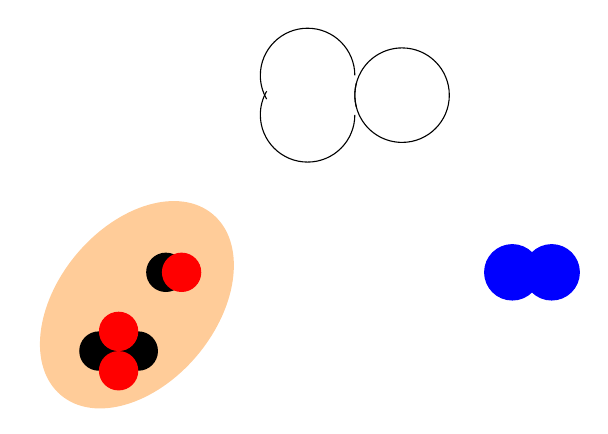
\begin{tikzpicture}		
		\fill[orange, fill opacity=0.4] (0.6,0.2)[rotate = 50] ellipse (1.5 and 1.0);
		
		\fill[black] (0.25, 0) circle (0.25);
		\fill[black] (-0.25, 0) circle (0.25);
		\fill[red] (0, 0.25) circle (0.25);
		\fill[red] (0, -0.25) circle (0.25);
		
			
		\fill[black] (0.6, 1.0) circle (0.25);
		\fill[red] (0.8, 1.0) circle (0.25);
		
		
		%\filldraw [blue] (2,2) -- (2,3) -- (3, 3) -- (3, 2) -- (2,2);
			
		\draw (3,3) arc (0:-210:0.6);
		\draw (3,3.5) arc (0:210:0.6);
		
		\draw (4.2,3.25) arc (0:-195:0.6);
		\draw (4.2,3.25) arc (0:195:0.6);
		
		
		\filldraw[blue] (5, 1) circle (10pt);
		\filldraw[blue] (5.5, 1) circle (10pt);
		
		
		%\draw (4, 4.5) arc(0:-300:0.6)  ;
		
		%\filldraw [green] (3, 3) circle (0.05) ;
		%\filldraw [blue] (4, 4.5) circle (0.05) ;
		
	\end{tikzpicture}
\end{center}

	\caption[Clustered $\mathrm{{}^{6}Li}$ nucleus]{Artistic representation of a clustered $\mathrm{{}^{6}Li}$ nucleus. The nucleus covers a two cluster system with an $\alpha$ particle and a deuterium as its constituencies.  }
	\label{fig:microscopical_cluster}
\end{figure}


An example of clustering is given with the $\mathrm{{}^{6}Li}$ nucleus depicted in Figure \ref{fig:microscopical_cluster}. With this picture, it is observed how the number of interacting bodies has decreased from 6 nucleons to 2 clusters: the  $\mathrm{{}^{4}He}$ and deuterium nucleus.  \\

Additionally, it is said that the $\alpha$ particle and the deuterium nucleus are the core and the valence clusters respectively. This classification is analogous to the core and valence electrons used in atomic physics. In particular, the core corresponds to the $\alpha$ particle cluster since it has more nucleons than the valence cluster which is the $d$ nucleus.  \\

On the other hand, in order to give this kind of models physical significance, selected interactions between clusters are introduced. The $NN$ and $NNN$ forces are standard examples of such needed interactions. In addition, since the constituents usually have many nucleons, extended object parameters like mass and charge density distributions may be encountered. \\

The mass and nuclear density of the nuclei can be modeled as a Woods-Saxon distribution as follows:

\begin{equation} \label{eq:micro_density}
	\rho(r) = \frac{\rho_0}{1 + \exp{\left(\frac{r - R}{a}\right)}}.
\end{equation} 


\subsubsection{RGM and GCM } \label{ssub:micro_RGM_GCM}

Microscopical cluster light nuclei study is also applied for more general systems \cite{freer_horiuchi_kanada-enyo_lee_meisner_2018}. The general approach when introducing microscopical cluster models is to construct a composite state $\Phi(\vec S_1, ..., \vec S_n)$ on top of the antisymmetrization of the product of the clusters which constitute the nuclei. An expression consistent with the previous description is given by:

\begin{equation}\label{eq:micro_cluster_generalizedWaveFunction}
	\Phi(\vec S_1, ..., \vec S_n)  = N \hat {\mathcal {A}} \{ \phi_1 (\vec S_1) ...  \phi_n (\vec S_n)\}.
\end{equation}

with $N$ as appropriate normalization constant, which usually is set to $1/\sqrt{A!}$ when all nucleons are considered within the model. Additionally, the variables $\vec S_1, ..., \vec S_n$ are interpreted as the relative positions of the clusters with respect to the center of the nuclei.  \\

Then, microscopic cluster calculations are splitted in two main approaches. On the one hand,  the resonant group method (RGM) provides a picture of the state of the nucleus $	\Psi_{\mathrm{RGM}}$ as being composed on the cluster states and an intercluster wave function. Particularly, the state is give by:

\begin{equation}\label{eq:micro_cluster_RGM_waveFunction}
	\Psi_{\mathrm{RGM}} =  \hat {\mathcal{A}} \{\phi_1 \phi_2 \zeta (\xi) \},
\end{equation}

where $\xi$ is a parameter that permits the description of the intercluster coordinate system. \\

On the other hand, an alternative method uses a more extended approach and exploits the use of the relative position vectors $\vec S_1, ..., \vec S_n$. This way of proceed in labeled as generator coordinate method  (GCM) and the expression of the state calculated by this approach $	\Psi_{\mathrm{GCM}}$ is expressed as: 

\begin{equation}\label{eq:micro_cluster_GCM_waveFunction}
	\Psi_{\mathrm{GCM}} = \int f(\vec S_1, ..., \vec S_n) \hat P \Phi(\vec S_1, ..., \vec S_n) d\vec S_1 ... d\vec S_n,
\end{equation}

where the function $ f(\vec S_1, ..., \vec S_n) $ is estimated with intrinsic information about the structure of the nuclei. \\

\subsubsection{Connection formulas} \label{ssub:connectionFormulas}

A more detailed survey on cluster models \cite{beck_2012}. There are equivalent relations between the RGM and GCM models, the two principal models of the cluster approach. The wave function of a state can be given as

\begin{equation}\label{eq:micro_cluster_equivalency_RGM}
	\Psi = \Phi^{-1}_{cm} \int f(R) \Phi(R) dR,
\end{equation}

where $\Phi^{-1}_{cm}$ corresponds to the center of mass wave function and $f(R)$ is a factor referred as the generator function. This is the picture given within the generate coordinate method (GCM). \\

The alternative picture is by the resonance group method, which is descete and is formulated as:

\begin{equation}\label{eq:micro_cluster_equivalency_GCM}
	\Psi = \hat{\mathcal{A}} \psi_1 \psi_2 g(r), 
\end{equation}

with the function $g(r)$, which is responsible for overlapping consideration, has the form of the integral: 

\begin{equation}\label{eq:micro_cluster_equivalency_GCM_g}
	g(r) = \int f(R) \Gamma(r, R) dR,
\end{equation}

where $\Gamma(r, R)$ serves as the kernel of the transformation that defines the $g(r)$ function. Then, it is possible to conclude that both methods seems to be similar as they are described by a single integration. The generator function is estimated with the Hill-Wheeler approximation, as it permits a determination of the penetration factor, which is closely related with the $\Gamma(r, R)$ parameter. \\

Additionally, this $g(r)$ term may be discretized and approximated by a series as given by: 

\begin{equation}\label{eq:micro_cluster_equivalency_GCM_g_series}
	g(r) = \sum_n f(R_n) \Gamma(r, R_n),
\end{equation}

where $n$ is the index running though all the estimations. For the specific case of a two clusters, the $\Gamma(r, R)$ term might be expanded as an expression compatible with a partial waves expansion. More concretely, the formula is:

\begin{equation}\label{eq:micro_cluster_gamma}
	\Gamma(r, R) = 4\pi \sum_{lm} {\Gamma_l(r, R) Y^{l}_m(\Omega_r) Y^{l}_{m*}(\Omega_r)},
\end{equation}

with $\Omega_r$ as the generalized solid angle and $l$ and $m$ as the secondary and azimuthal quantum numbers. The generator function, within this framework, can be then defined as the solution of the equation: 

\begin{equation}\label{eq:micro_cluster_g_equation}
	\int [H_l(R, R') - E N_l(R, R') f_l(R')] dR' = 0.
\end{equation}

A minimization condition is settled. The particular expressions of the matrix elements are $ H_l(R, R') = \langle  \Phi(R) | H | \Phi(R') \rangle $ and $ N(R, R') = \langle  \Phi_l(R) | \Phi_l(R') \rangle $. \\


\subsubsection{Hyperspherical model}\label{ssub:micro_cluster_hyperspherical}

Break up effects for four to five body model can be also addressed. This phenomena is relevant when considering collision of middle to heavy nuclear reactions. The following description follows closely the approach to the model made by  \cite{shubhchintak_descouvemont_2022}. The hyperspherical coordinates, which are useful when describing the effects of clustering, are frequently parametrized with the Jacobi $\vec x$ and $\vec y$ coordinates. In particular, this was used for a nucleus with the form $C + n + n$. Namely, with one core $C$ and two neutrons $n$. \\

When introducing the Schrödinger equation for this kind of cluster approaches, it is necessary to modify the kinetic energy operator. If cylindrical like coordinates for the  $(\rho, \phi')$ are used, with 

\begin{equation}\label{eq:micro_cluster_breakup_rho}
	\rho = \sqrt{x^2 + y^2}
\end{equation}

and with 

\begin{equation}\label{eq:micro_cluster_breakup_phi}
	\phi' = \arctan \left( \frac{y}{x}\right),
\end{equation}


Their eigenfunctions of the generalized kinetic operator are defined as: 

\begin{equation}\label{eq:micro_cluster_breakup_hyperspherical}
	\mathcal{Y} = \phi (\phi') [Y^{l_x}(\Omega_x) \otimes Y^{l_y} (\Omega_y)],
\end{equation}

where $l_x$ and $l_y$ are the angular momentum values for $\vec x$ and $\vec y$ while $\phi$ corresponds to a wave function which is defined as: 

\begin{equation}\label{eq:micro_cluster_breakup_wavefunction}
	\phi(\phi')  = C (\cos \phi')^{l_x}   (\sin \phi')^{l_y} P_n^{l_y + 1/2, l_x + 1/2} \cos (2\phi'),
\end{equation}

where $C$ is a normalization constant and the polynomials $P_n^{l_y + 1/2, l_x + 1/2} \cos (2\phi')$ are generalizations of the Legendre with a particular form. The integer $n$ is defined as: 

\begin{equation}\label{eq:micro_cluster_breakup_n}
	n = \frac{K - l_x - l_y}{2},
\end{equation}

where $K$ plays the role of a fifth dimensional angular momentum. Also, a more general hyperspherical harmonics can be introduced by considering the spin of external neutrons. More concretely, when the spinor $\chi$ is introduced, the modified spherical harmonics $\mathcal{Y}'$ is given by 

\begin{equation}\label{eq:micro_cluster_breakup_hyperspherical_spinor}
	\mathcal{Y}^{jm}_{\nu K}(\Omega) = [\mathcal{Y}^{l_xl_y}_{KL} \otimes \chi^{S}]^{jm}.
\end{equation}

With the previous picture considered, the wave function, for a three body interaction, is expressed as: 

\begin{equation}\label{eq:micro_cluster_breakup_wavefunction_complete}
	\Psi^{jm\pi} = {\rho}^{-5/2} \sum_{K} \sum_{\nu} {\chi^{j\pi}_{\nu K} (\rho) \mathcal{Y}^{jm}_{\nu K} (\Omega_{\rho})}.
\end{equation}

Usually the series is truncated at $K'$. On the other hand, the radial functions $\chi$ are solutions to the scattering-like differential equation: 

\begin{equation}\label{eq:micro_cluster_breakup_differentialEquation}
	\left[ -\frac{\hbar^2}{2m} \left( \frac{d^2}{d\rho^2} - \frac{(K + 3/2)(K + 5/2)}{\rho^2}  \right)   \right ] \chi^{j\pi}_{\nu K} (\rho)   + \sum_{\nu' K'} V^{j\pi}_{\nu' K', \nu K}(\rho) \chi^{j\pi}_{\nu'K'}(\rho) = E^{j\pi}  \chi^{j\pi}_{\nu K}.
\end{equation}

Notice that the difference between primed (incident) and non-primed (outgoing) quantum numbers make equation \ref{eq:micro_cluster_breakup_differentialEquation} to be coupled. Additionally, $V^{j\pi}_{\nu' K', \nu K}$ represents the matrix elements of the two-potential. Additionally, since this picture is fifth dimensional and includes spin, the term $(K + 3/2)(K + 5/2)$ differs to the three dimensional analogous $l(l +1)$ description as it contains higher and fractional numbers $3/2$ and $5/2$ in contrast to the $0$ and $1$ for the traditional quantum mechanical picture. \\

\subsubsection{More applications} \label{ssub:micro_cluster_moreApplications}

An application of microscopical cluster theory can be found in systems like $\mathrm{{}^{12}C}$ and $\mathrm{{}^{24}Mg}$ which can be modeled as a three cluster nuclei with the form $\alpha + \alpha + \alpha$ and $\mathrm{{}^{16}O + \alpha + \alpha}$ respectively  \cite{descouvemont_2021}. The Jacobi coordinates for the three body model are given as: 

\begin{equation}\label{eq:middleFusion_threeBody_cluster_x}
	\vec x = \sqrt{ \frac{A_1A_2}{A_1 + A_2}} \vec r 
\end{equation}

and 

\begin{equation}\label{eq:middleFusion_threeBody_cluster_y}
	\vec y = \sqrt{ A_c\frac{A_1 + A_2}{A_c + A_1 + A_2}} \vec R, 
\end{equation}

where $A_c$, $A_1$ and $A_2$ correspond to the mass numbers of the core and the valence clusters respectively. Then, the wave function assumes the shape: 

\begin{equation}\label{eq:middleFusion_threeBody_waveFunction}
	\Psi^{JM\pi} = \sum_{l_xl_y} \sum_{K = 0}^{\infty} { \hat{ \mathcal{A}} {\phi_1 \phi_2 \phi_3} \otimes  \mathcal{Y}^{l_x l_y}_{KJM}(\Omega^4) \chi^{J\pi}_{l_x l_y K}(\rho)}.
\end{equation}

There are various approaches to include resonances. One is to introduce a rotation in position and momentum space. This converts the Schrödinger equation as: 

\begin{equation}\label{eq:middleFusion_threeBody_resonances_rotation}
	H(\theta) \Psi (\theta) = E(\theta) \Psi (\theta),
\end{equation}

where $\theta$ corresponds to the rotation angle. The advantage of this strategy, which is referred as the complex scaling method, is that states with resonances are not affected by the transformation. Particularly, the eigenvalues are given by: 

\begin{equation}\label{eq:middleFusion_threeBody_resonances_rotation_eigenValues}
	E(\theta) = E_R - i \frac{\Gamma}{2},
\end{equation}

where $E_R$ and $\Gamma$ correspond to the energy peak and width of the resonances.\\

Alternatively, under the complex absorbing potential method, the Hamiltonian can be modified by introducing a new term accountable for the resonant behavior. Such transformation has the form: 

\begin{equation}\label{eq:middleFusion_threeBody_resonances_complexAbsorption}
	H(R', R) \rightarrow H(R, R') - i \eta W(R) \delta(R - R'),
\end{equation}

with the complex potential term as: 

\begin{equation}\label{eq:middleFusion_threeBody_resonances_complexAbsorption_potential}
	W(R) = \theta(R - R_0) (R - R_0)^{\beta},
\end{equation}

where $R_0$ relates to a radius free parameter and $\theta$ corresponds to the step function and the exponent $\beta = 4$ usually. \\

$NN$ forces included with additional aspects of the study of microscopic models for the context of study of the deuterium reactions $\mathrm{{}^{2}H(d, \gamma){}^{4}He}$, $\mathrm{{}^{2}H(d, p){}^{3}H}$ and $\mathrm{{}^{2}H(d, n){}^{3}He}$ reactions \cite{arai_aoyama_suzuki_descouvemont_baye_2013}. One of such approaches towards cluster models was based on the resonating group method (RGM) with the Minnesota potential, which accounts for the tensor force effect of the aforementioned reactions. A multichannel behavior was incorporated in the model. \\

Another application can be found in the context of  $\Cfusion$ (3$\alpha$) \cite{dufour_descouvemont_1997}. Middle heavy nuclei can be modeled as cluster collections. In the case of $\mathrm{{}^{12}C}$, it corresponds to $3 \alpha$. Then, the carbon nucleus is regarded as a compounded system of three identical particles. Cluster approach permits a description of the systems as a triangle conformed by the three alpha particle and parametrized by position like variables coordinates $\vec S_1 $, $\vec S_2$ and $\vec S_3$. Then, the $\mathrm{{}^{12}C}$ wavefunction $\Phi_{3\alpha}$ is expressed within this formalism as: 

\begin{equation}\label{eq:micro_multicluster_3alpha}
	\Phi_{3\alpha} = \hat {\mathcal{A}} \left\{ \Phi_\alpha (\vec S_1) \Phi_\alpha(\vec S_2) \Phi_\alpha(\vec S_3) \right\},
\end{equation}

where $\Phi_\alpha (\vec S_1)$,   $\Phi_\alpha (\vec S_2)$ and 
$\Phi_\alpha (\vec S_3)$ are the wavefunctions for the three alpha clusters. Then, since these are fermionic-like indistinguishable particles, the antisymmetrization operator  $\hat {\mathcal{A}} $ was introduced. \\

An interaction with a nucleon with a three cluster system requires the introduction of an additional variable $\vec R$, which accounts for the position from, approximately, the center of the triangle to the nucleon. The picture of the composite state related to the last description has the form: 

\begin{equation} 	\label{eq:micro_multicluster_abc}
	\Phi^{N}_{3\alpha} = \Phi_\alpha \left (-\frac{1}{13} \vec R + \vec S_1 \right )  \Phi_\alpha \left (-\frac{1}{13} \vec R + \vec S_2 \right )  \Phi_\alpha \left (-\frac{1}{13} \vec R + \vec S_3 \right )  \Phi_N \left( \frac{12}{13} \vec R \right),
\end{equation}

where $\Phi_N$ corresponds to the wave function of the nucleon $N$ and the center or core like $3\alpha$. The exact form of $\vec S_1$, $\vec S_2$ and $\vec S_3$ depends on the spacial orientation of the cluster. Since it involves rotations in various planes, a better picture of the state of the system is given by:

\begin{equation} 	\label{eq:micro_multicluster_eulerAlgles}
	\Omega = (\alpha, \beta, \gamma),
\end{equation}

where the triple $\Omega$ is determined by the Euler angles $\alpha$, $\beta$ and $\gamma$. \\

\section{Matrix models}  \label{sec:matrixModels}

The matrix models permit approaching of resonances with an appropriate fitting of free parameters. In particular, the main formalism in this approach is the R-matrix model. A classical and more reviews are found in the  \cite{lane_thomas_1958} and \cite{descouvemont_baye_2010}. \\

\subsection{Calculable R-matrix} \label{sub:rmatrix_calculable}

This section is inspired to a great extent on the R-matrix review paper by Descouvemont \& Baye \cite{descouvemont_baye_2010}. The approach of this part is to present the coupled channel picture relevant to the theory. Later, R-matrix definitions will be presented. Then, an some concepts related to Coulomb scattering will be reviewed and expanded. Next, relevant aspects of radiative capture calculations will be included. Finally, an application example will be developed.

\subsubsection{Coupled channels picture} \label{ssub:rmatrix_calculable_coupled_channels}

In order to describe the state of the system $	|c\rangle$ of coupled internals states is given by: 

\begin{equation}\label{rmatrix_channels_state}
	|c\rangle = i^{l_c} [[\phi^{(1)}_{cI_1} \otimes  \phi^{(2)}_{cI_2}]_{I_c} \otimes Y_{l_c}(\Omega_c) ]^{(JM\pi)},
\end{equation}

where the two wave functions $\phi^{(1)}_{cI_1}$ and $\phi^{(2)}_{cI_2}$ are coupled with the direct product. They have associated spins which are labeled as $I_1$ and $I_2$, as well as a channel spin $I_c$, which is the result of the addition of the previous angular momenta. Additionally, the spherical harmonics $Y_{l_c}(\Omega_c)$ is parametrized with the solid angle $\Omega_c$ and with the relative angular momentum number $l_c$. All the previous variables are considered within the framework of transitioning to the $J, M$ angular momentum basis with parity $\pi$. \\

Additionally, an orthonormality condition is imposed for the channel states, which is expressed as: 

\begin{equation}\label{rmatrix_channels_orthonormality}
	\langle c| c' \rangle = \delta_{cc'}.
\end{equation}

The composite system is going to be thus formed as a combination of the channel states. More concretely, this is given by: 

\begin{equation}\label{rmatrix_channels_systemState}
	\Psi(r_c) = \sum_{c} \hat {\mathcal{A}} |c \rangle \frac{u_c}{r_c}(r_c),
\end{equation}

where $\hat{\mathcal{A}}$ corresponds to the antisymmetrization operator. Then, when this wave function is considered in the Schrödinger equation, a coupled channel equation arises, which corresponds to the expression:

\begin{equation}\label{rmatrix_channels_coupledEquation}
	[T_c + V_c(r) + E_c - E]u_c(r) + H =0,
\end{equation}

where $T_c$ is the kinetic operator defined as:

\begin{equation}\label{rmatrix_channels_kineticOperator}
	T_c = -\frac{\hbar^2}{2\mu_c} \left(\frac{d^2}{dr^2} - \frac{l_c(l_c + 1)}{r^2}\right).
\end{equation}

Also, the term $V_c(r)$, which corresponds to the matrix elements of the local potential, is given by:

\begin{equation}\label{rmatrix_channels_V}
	V_c(r) = \langle c | V | c \rangle. 
\end{equation}

Additionally, the term $H$ corresponds to the non local part of the potential, which is given in the terms of:

\begin{equation}\label{rmatrix_channels_nonLocal}
	H = \sum_{c'}{\int_{0}^{\infty} W_{cc'}(r, r')u_{c'}(r') dr'},
\end{equation}

with $W_{cc'}$ even further defined as: 

\begin{equation}\label{rmatrix_channels_nonLocal_W}
	W_{cc'}(r, r') = \langle c | \delta (r_c - r) V \hat{\mathcal{A}} \delta (r_{c'} - r')|  c' \rangle - V_c(r)\delta_{cc'}\delta (r- r'),
\end{equation}

where $V_c(r)$ labels a channel potential and $V$ corresponds to the many body potential, which may take into account NN interactions. \\

\subsubsection{R-matrix definition and parametrization} \label{ssub:rmatrix_calculable_definition_parametrization}


Solution of the Bloch-Schrödinger equation with the form of a Green's function equation:

\begin{equation}\label{rmatrix_BlochSchrodinger}
	(H_l + \mathcal{L}(B) - E)G_l(r, 'r) = \delta(r - r'),
\end{equation}

where the operator $\mathcal{L}(B)$, which is known as the surface Bloch operator,  is given by:

\begin{equation}\label{rmatrix_Bloch_operator}
	\mathcal{L}(B) = \frac{\hbar^2}{2\mu} \delta(r - a) \left(\frac{d}{dr} - \frac{B}{r}\right),
\end{equation} 

with $B$ as the boundary parameter which is frequently introduced within the R-matrix formalism. \\


With the last terms just presented, the R-matrix is specifically defined as: 

\begin{equation}\label{rmatrix_Bloch_rmatrix}
	R_l(E) = \frac{\hbar^2}{2\mu a} G_l(a, a).
\end{equation} 

Alternatively, the R-matrix is given by:

\begin{equation}\label{rmatrix_u_rmatrix}
	R_l(E) =  \frac{u_l(a)}{au'_{l}(a) - Bu_l(a)}.
\end{equation} 

Then, the wave function, which is a solution of the inhomogeneous Green's function differential equation is given by:

\begin{equation}\label{rmatrix_BlochSchrodinger_inhomogeneous}
	(H_l + \mathcal{L}(B) - E)u^{\mathrm{(Int)}}_l = \mathcal{L}(B) u^{\mathrm{(Ext)}}_l ,
\end{equation}

with the continuity conditions on both the radial wave function and its first order derivative. Then, the internal wave function is given as:

\begin{equation}\label{rmatrix_Bloch_internalWaveFunction}
	u^{(\mathrm{Int})}_l(r) = \int_{0}^{a} G_l(r, r') \mathcal{L}(B) u^{\mathrm{Ext}} (r') dr'.
\end{equation} 


\subsubsection{Coulomb asymptotic behavior} \label{ssub:rmatrix_calculable_coulomb}

This discussion starts as an extension of the Coulomb scattering section \ref{ssub:scattering_coulomb}. One of the main consequences of this incorporation is a change on the shape of the asymptotic behavior. More particularly, the incoming term Coulomb term is given by:

 \begin{equation}\label{rmatrix_channels_incomingCoulomb}
 	\Psi_{1C}(r) \rightarrow  \psi_C\phi^{(1)}_{cI_1} \phi^{(2)}_{cI_2}.
 \end{equation}

Meanwhile, the outgoing term has the form:


\begin{equation}\label{rmatrix_channels_outgoing}
	\Psi_{2C}(r) \rightarrow \frac{1}{(2\pi)^{3/2}} \sum_{c' \alpha} \frac{\exp {[i(k_{c'}r - \eta_{c'} \ln {(2k_{c'}r )})]}}{r} f^{c\alpha}_{c'\alpha'}(\Omega)  \phi^{(1)}_{cI_1} \phi^{(2)}_{cI_2},
\end{equation}

where $\alpha$ correspond to a set of quantum numbers that would fully parametrize the states of the system. Therefore, the final state $\Psi$ is approached by: 

\begin{equation}\label{rmatrix_channels_state_final}
	\Psi(r) \rightarrow \Psi_{1C}(r) + \Psi_{2C}(r).
\end{equation}

The function can be further expanded and it could include a change of basis. More particularly, the modified state $	\overline \Psi(r)$ may be written as:

\begin{equation}\label{rmatrix_channels_state_final_change}
	\overline \Psi(r) = i \frac{\pi^{1/2}}{(2\pi)^{3/2} k} \sum_{J\pi} \sum_{Il} C^{-1}_c \sqrt{2l + 1} \exp (i\sigma_l) K \Psi(r),
\end{equation}

where $\Psi(r)$ corresponds to the solution of equation \ref{rmatrix_channels_systemState} and $K$ is defined in terms of Clebsh Gordan coefficients as: 

\begin{equation}\label{rmatrix_channels_state_final_clebshGordan}
	K = \langle I_1 I_2 M_1 M_2 | IM\rangle \langle IlM0 | JM\rangle.
\end{equation}


The reduced differential cross section for the inlesatic process $c\rightarrow c'$ is given by:

\begin{equation}\label{rmatrix_difcrossSection_ccprime}
	\frac{d\sigma_{c\rightarrow c'}}{d\Omega} = C \sum_{\alpha} \sum_{\alpha'} |f^{c\alpha}_{c'\alpha'}|^2,
\end{equation}

where the spin constant $C$ is defined as:

\begin{equation}\label{rmatrix_difcrossSection_spinConstant}
	C = \frac{1}{(2I_1 + 1)(2I_2 + 1)},
\end{equation}

where $I_1$ and $I_2$ correspond to the spin values of the reactants and products. They account for the spin degeneracy correction. \\

Now, the expression of the cross section is given in terms of the collision matrix as:

\begin{equation}\label{rmatrix_crossSection_ccprime}
	\sigma_{c\rightarrow c'} = \frac{\pi}{k^2} C \sum_{J\pi} {(2J +1) \sum_{Il} \sum_{I'l'} |U^{J\pi}_{c'I'l'cIl}|^2},
\end{equation}

with $J$ and $\pi$ as the total angular momentum and parity quantum numbers and $I$ and $I'$ as the incoming and outgoing channel angular momentum number. Reciprocally, $l$ and $l'$ holds for the reciprocal angular momentum number of the $c$ and $c'$ channels respectively.\\

\subsubsection{Radiative capture reaction considerations} \label{ssub:rmatrix_calculable_radiative_capture}

In the specific case of radiative capture, the collision matrix is given by: 

\begin{equation}\label{rmatrix_radiativeCapture_U}
	U = \sqrt{\frac{2J_f + 1}{2J + 1}} A \frac{\langle \Psi^{J_f\pi_f} || \mathcal{M}^{\sigma \lambda} ||  \Psi^{J \pi}_{Il} \rangle }{C_{Il}},
\end{equation}

where the term $A$ is given by:

\begin{equation}\label{rmatrix_radiativeCapture_A}
	A = \sqrt{\frac{8\pi(\lambda + 1)}{\hbar v \lambda [(2\lambda + 1)!!]^2}}.
\end{equation}

It is possible to reduce the transition matrix elements. Particularly, by using the Wigner-Eckart, the matrix element is given by:

\begin{equation}\label{rmatrix_radiativeCapture_transitionMatrix}
	\langle \Psi^{J_fM_f\pi_f} | \mathcal{M}^{\sigma \lambda}_\mu |  \Psi^{J M \pi}_{Il} \rangle = (J\lambda M \mu | J_fM_f) \langle \Psi^{J_f\pi_f} || \mathcal{M}^{\sigma \lambda} ||  \Psi^{J \pi}_{Il} \rangle,
\end{equation}

where $\mu$ is an index of a component of the non-reduced matrix element $\mathcal{M}^{\sigma \lambda}_{\mu}$, which is analogous to the role that $m$ plays in classical angular momentum description. The general form of the amplitude for electric transitions is given by: 

\begin{equation}\label{rmatrix_radiativeCapture_M}
	\mathcal{M}^{E\lambda}_{\mu} = eZ^{(E\lambda)}_{\mathrm{eff}} r^{\lambda} Y^{\lambda}_{\mu} (\Omega),
\end{equation}

with $e$ the electric charge and the effective charged $Z^{(E\lambda)}_{\mathrm{eff}}$ defined as: 

\begin{equation}\label{rmatrix_radiativeCapture_effectiveCharge}
		Z^{(E\lambda)}_{\mathrm{eff}} = Z_1\left(- \frac{m_2}{m}\right)^{\lambda} + Z_2 \left(\frac{m_1}{m}\right)^{\lambda}.
\end{equation}

On the other hand, the reduced matrix is given by: 

\begin{equation}\label{rmatrix_radiativeCapture_reducedMatrix_expression}
	\langle \Psi^{J_f\pi_f} || \mathcal{M}^{\sigma \lambda} ||  \Psi^{J \pi}_{Il} \rangle = e \frac{Z^{(E\lambda)}_{\mathrm{eff}}}{\sqrt{4\pi (2J_f + 1)}} \sum_{I_fl_fl_0}(-1)^{I_f - J} Z \int_0^{\infty} {u^{J_f}_{I_fl_f}(r) r^\lambda u^{J}_{I_fl_0} (r)dr}, 
\end{equation}

with the coefficients $Z$ defined as: 

\begin{equation}\label{rmatrix_radiativeCapture_Zcoefficients}
	Z = (-1)^{J + J'} \sqrt{(2\lambda + 1)(2J+ 1)(2J' + 1)(2l + 1)(2L + 1)} K ,
\end{equation}

where the term $K$ is terms of 3j and 6j symbols as: 

\begin{equation}\label{rmatrix_radiativeCapture_3j6j}
	K  = \left(\begin{matrix}
		l & L & \lambda \\
		0 & 0 & 0
	\end{matrix}\right) \left\{ \begin{matrix}
		l & L & \lambda \\
		J' & J & I
\end{matrix} \right\}.
\end{equation}

\subsubsection{Calculation application} \label{ssub:rmatrix_calculable_calculationapplication}

The wave function can be splitted in two parts. One represents the behavior behind the boundary with $r < a$, which is named as $u^{(\mathrm{Int})}$ while the other accounts for above the barrier radial part $u^{(\mathrm{Ext})}$. The total is given by: 

\begin{equation}\label{rmatrix_internal_external}
	u_l = u^{(\mathrm{Int})}_l +  u^{(\mathrm{Ext})}_l.
\end{equation} 

With respect to asymptotic expressions, the external function has the form: 

\begin{equation}\label{rmatrix_external_asymptotic}
	u^{(\mathrm{Ext})} = C_l [I_l(kr) - U_l O_l(kr)],
\end{equation} 

while the internal has the form of a superposition of bounded wave functions, which is expressed as: 

\begin{equation}\label{rmatrix_internal_asymptotic}
	u^{(\mathrm{Int})} = \sum_{l=0}^{N} c_k \phi_k(r),
\end{equation} 

where the set of functions $\{\phi_k(r)\}$ serves as a basis for the internal solutions. Some specific shapes for these functions may be conveniently selected to reproduce cross section data. \\

When it comes to defining details on radiative capture calculations, it is necessary to compute the transition elements of the form $\langle u_f | r^\lambda| u \rangle $, with $u_f$ as the final wave function state and $u$ as the initial wave function. This computation process follows as:

\begin{equation}\label{rmatrix_radiativeCapture_integral}
	\langle u_f | r^\lambda| u \rangle  = \int_0^{\infty} u_f r^\lambda u  dr =  \int_0^{a} u_f^{(\mathrm{Int})} r^\lambda u^{(\mathrm{Int})}  dr + \int_a^{\infty} u_f^{(\mathrm{Ext})} r^\lambda u^{(\mathrm{Ext})}  .
\end{equation}

This integral can be solved by considering both the internal and external contributions related to the wave function. For the former, the integral can be approximated as: 

\begin{equation}\label{rmatrix_radiativeCapture_integral_internal}
	\int_0^{a} u^{(\mathrm{Int})}_f r^\lambda u^{(\mathrm{Int})}  dr  = \sum_{k, k'} c_{f, k'} c_{k} \int_0^{a} \phi_{k'} r^\lambda \phi_{k}dr, 
\end{equation}

where $k$ and $k'$ correspond to the wave numbers of the contributions of the incoming and outgoing channels. Additionally, as the computation is restricted to the region $r < a$, the integral of the right of equation \ref{rmatrix_radiativeCapture_integral_internal} is evaluated with the bounded wave functions $\phi$. \\

On the other hand, for the external computations, the expression is given as: 


\begin{equation}\label{rmatrix_radiativeCapture_integral_external}
	\int_a^{\infty} u^{(\mathrm{Ext})}_f r^\lambda u^{(\mathrm{Ext})}  dr = C C_f \int_a^{\infty} W (2\kappa r) r^{\lambda} (I(kr) - U O(kr)) kr, 
\end{equation}

where $\kappa$ is a variable associated with the wave number of external states. Additionally, the scattered picture was given by using the incoming and outgoing wave functions. 

\subsection{Phenomenological R-matrix} \label{sub:rmatrix_phenomenological}

Obtaining the R-matrix from the Schrödinger equation is usually a complex task. In particular, when the number of channels grow, the R-matrix functions are more challenging to compute. This complexity issue motivates the need of an approach which leans to simplifying the formalism.  \\

\subsubsection{Motivation} \label{ssub:rmatrix_phenomenological_motivation}


Instead of solving the Schrödinger equation, it is possible to obtain specific formulas that account for the R-matrix  behavior up to a certain degree of certainty.  \\

The broad idea of this approach is to parametrize the scattering states of system.  The model includes free parameter $a$ which is called the radius channel. This serves as an estimated value such that at radius $r > a$ the electromagnetical interaction becomes relevant, which is where the radiative region is located. In contrast, in the interior region, with $r < a$, the nuclear force is the dominant interaction. \\

Additionally, boundary conditions are added as an external input. Recall that at the boundary, where $r = a$, the solution to the logarithmic derivative of the Schrödinger equation is imposed to be continuous since this condition implies simultaneous continuity on both the wave function and its first order derivative. Then, an non-dimensional quantity $f$, which is closely related with the logarithmic derivative, is introduced and it is defined as \cite{iliadis_2015}:

\begin{equation}\label{eq:rmatrix_f}
	f = a\left.\frac{1}{u(r)} \frac{du(r)}{dr}\right|_{r = a}.
\end{equation}

With the channel radius defined, the value of $f(r = a)$ is fixed as a boundary condition, which is usually referred as $B$.  Then, these parameters are also considered as free since they are adjusted. This value allows to define an specific parametrization of the variables of the reaction. \\

Next, $f$ can be expanded in power series as following: 

\begin{equation}   \label{eq:rmatrix_f_powerSeries}
	f(r) = f(a) + \left.\frac{df}{dr}\right|_{r = a} (r - a) +  \frac{1}{2!} \left.\frac{d^2f}{dr^2}\right|_{r = a} (r - a )^2  ... \ .
\end{equation}


Since the formulation of the R-matrix is strongly inspired by the modeling of resonant reactions, a natural starting point is the Breit-Wigner approximation. Particularly, when angular momentum $l$ is considered, the cross section associated to a single resonance is expressed as:

\begin{equation}  \label{eq:rmatrix_breitWigner}
	\sigma = \frac{\pi}{k^2} \sum_{l} (2l + 1) \frac{\Gamma^{(1)}_{l} \Gamma^{(2)}_{l} }{(E - E_l)^2  + \Gamma^2_l }, 
\end{equation}

where $k$ is the wave number, $E_l$ is the energy peak,  $\Gamma^{(1)}_{l}$ and $\Gamma^{(2)}_{l}$ are the partial widths for the reactant species and $\Gamma$. summed and then averaged corresponds to the total width, which is defined as: 

\begin{equation}  \label{eq:rmatrix_totalWidth}
	\Gamma_l = \Gamma^{(1)}_{l} + \Gamma^{(2)}_{l}. 
\end{equation}


Within the Breit-Wigner formalism, the energy peak and the width can be expressed terms of $f$. Before introducing the exact form of the relation, it is necessary to define additional variables that would help to expressed the aforementioned physical observable quantities.  \\

One of such variables is the penetration factor $P_l$, which is defined as: 

\begin{equation}  \label{eq:rmatrix_penetrationFactor}
	P_l = \frac{a}{(k_1 f(r = a ))^2 + \left(k_2 \left.\frac{df}{dr}\right|_{r = a} \right)^2 }.
\end{equation}

This parameter is useful when expression the reaction width as: 

\begin{equation}   \label{eq:rmatrix_width_penetration}
	\Gamma_l = 2C_l\gamma^2_l,
\end{equation}

where $\gamma$ is another variable named as reduced width,  which is defined as: 

\begin{equation}   \label{eq:rmatrix_reducedWidth}
	\gamma_l = \left(\frac{\partial f}{\partial E}\right)^{-1}_{E_\lambda}
\end{equation}


Then, equations \ref{eq:rmatrix_width_penetration} and \ref{eq:rmatrix_reducedWidth}  where obtained by approximating $f$ up to first order in the expansion.\\

\subsubsection{R-matrix and related definitions} \label{ssub:rmatrix_phenomenological_definitions}

A convenient rearrangement of terms can converge to the definition of a special variable, which is called the R-matrix, as: 

\begin{equation}  \label{eq:rmatrix_definition1}
	R= \sum_\lambda {\frac{\gamma_{\lambda c} \gamma_{\lambda c'}}{E - E_k}}, 
\end{equation}

where $\gamma_{\lambda c'} $ and $\gamma_{\lambda c}$ are quantities which would play an analogous, but not necessary exact, role to reduced widths. Similarly, the R-matrix poles $E_k$ are associated but not always equal to the energy peaks. \\

It is now possible to define the connections between the observed, in the experimental sense, and their correspondent R-matrix parameters. Then, a pole of the matrix $E_\lambda$ differs from the actual experimental value $E_l$ as:

\begin{equation}  \label{eq:rmatrix_energyPole}
	E_\lambda =  E_l - \Delta, 
\end{equation}

where the energy shift is given by: 

\begin{equation}  \label{eq:rmatrix_energyShift}
	\Delta = -(S_c(E) - B_c)\gamma_{\lambda c}.
\end{equation}

At this point, it is worth to be noticed that $S_l = 0$ for the case of uncharged reaction pictures. Then, for such situations, $E_\lambda = E_l$ holds and therefore there the energy pole and the actually observed energy peak are equivalent. However, within the R-matrix formalism, a shift appears when relating these two energy like terms in therms of $S_l$, which is frequently referred as the shift factor. \\

\subsubsection{Parametrizations} \label{ssub:rmatrix_phenomenological_parametrizations}

There is more than a single parametrization for matrix models \cite{brune_2002}. Usually the alternative formulations surge from the need to express the parameters of the model in order to facilitate the imposition of boundary conditions.  

\begin{equation}\label{eq:rmatrix_E}
	\mathcal{E} = e - \sum_{c}{\gamma_c \gamma^{T}_c (S_c - B_c)}.
\end{equation}

This matrix $\mathcal{E}$ obeys the eigenvalue equation:

\begin{equation}\label{eq:rmatrix_E_values}
	\mathcal{E}\vec a_k = E_k \vec a_k.
\end{equation}

The width in the formalism is given by:

\begin{equation}\label{eq:rmatrix_width}
	\Gamma_{kc} = \frac{2P_c \hat {{\gamma}^2_{kc}}}{1 + \sum_{c}{\hat {{\gamma}^2_{kc}} \left(\frac{dS_c}{dE}\right)_{\hat{E}_c}  }}.
\end{equation}

The symbols with $\hat {{\gamma}^2_{kc}}$ has the expression: 

\begin{equation}\label{eq:rmatrix_width_reduced}
	\hat {{\gamma}^2_{kc}} = a^{T}_{k} \gamma_c.
\end{equation}

Additionally, it is possible to simplify the last expressions by imposing: 

\begin{equation}  \label{eq:rmatrix_spacialboundaryCondition}
	B = f(r = a). 
\end{equation}

Then, with this parametrization, $\Delta = 0$ and thus the formal and width parameters become equivalent. Naturally, equation \ref{eq:rmatrix_spacialboundaryCondition} is usually  the preferred for R-matrix calculations. \\

\subsubsection{Empirical} \label{ssub:rmatrix_phenomenological_empirical}

It is possible to estimate the phase shift with the R-matrix formalism. There are two main contributions: the background, which is usually non-resonant, and the resonant. \\

The last introduction of the R-matrix for was based on the requisite of narrow resonance. However,  is possible to describe reactions with multiple channels and to generalize the assumptions made in the Breit-Wigner formalism with the same R-matrix definition. Particularly, extended resonances and non-resonant behavior can be also analyzed withing this theoretical framework.\\

Further approaches in the context of the R-matrix have different forms depending on the inclusion of effects of channels and spins. The first approximation is given by considering a single channel. Additionally, spin effects and the related formulae are included in the R-matrix formalism. Angular momentum and parity conservation can be included within R-matrix calculations. \\

Then, with all the variables considered, an empirical formula obtained from the R-matrix formalism is given by:

\begin{equation} \label{eq:rmatrix_sfactor}
	S(E) = S_r \frac{\Gamma^2/4}{(E-E_r + \Delta)^2 + (\Gamma/2)^2}.
\end{equation}

\subsection{Applications} \label{sec:Calculable R-matrix}

Applications of the R-matrix formalism to a wide range or reactions. Analytical formulas were used to describe the S-factor behavior of non resonant $\ddexchange$, $\mathrm{{}^{2}H(d, n){}^{3}He}$ reactions and the resonant behavior, with a formula inspired in the R-matrix formalism, of the $\mathrm{{}^{3}He(d,p){}^{4}He}$ (one resonance) and $\mathrm{{}^{7}Li(d, \alpha){}^{4}He}$ (two resonances) reaction \cite{sparta_pizzone_bertulani_hou_lamia_tumino_2020}. \\

Resonances arrives from poles. Deviations from Breit-Wigner resonance prediction. A description on the physical consideration of poles in the scattering (S-matrix) is given in \cite{ramirezjimenez_kelkar_2018}. For broad resonances, the Breit-Wigner formula can be expanded. Meaning that 

\begin{equation}\label{eq:rmatrix_generalizedBW}
	\sigma_l = \frac{4\pi(2l+1)}{\epsilon_{lr}} \frac{(\Gamma_{lr}/2 )^2}{(k^2 - \epsilon_{lr})^2 + (\Gamma_{lr}/2)^2} P \left(\frac{\Gamma_{lr}}{2\epsilon_{lr}}\right),
\end{equation}

where the term $P$ permits the expansion in Taylor series which effectively corrects the Briet-Wigner formula behavior as: 

\begin{equation}\label{eq:rmatrix_generalizedBW_expansion}
	P \left(\frac{\Gamma_{lr}}{2\epsilon_{lr}}\right) = 1 - \frac{1}{4} \left(\frac{\Gamma_{lr}}{2\epsilon_{lr}}\right)^2 + \frac{1}{8} \left(\frac{\Gamma_{lr}}{2\epsilon_{lr}}\right) ^4 + ... .
\end{equation}


In primordial nucleosynthesis, the R-matrix can be also applied in the framework of $\mathrm{{}^{3}He}$ reactions study  \cite{desouza_iliadis_coc_2019}. Analysis of the BNN reaction $\mathrm{{}^{3}He(d, p){}^{4}He}$. The model uses Bayesian analysis to improve parameter fitting. The likelihood of a parameter is given by:

\begin{equation}\label{eq:rmatrix_bayesian_likelihood}
	\mathcal{L}(S|\theta) = \prod_{k=1}^{N} \frac{1}{\sqrt{2\pi \sigma^2} } \exp {\left[- \frac{(S_k - S_k(\theta))}{2\sigma^2}\right]},
\end{equation}

where $\theta$ considers the parameters to be optimized and $S_k$ corresponds to experimental S-factor values. Likewise, Bayesian fitting methods are also common when implementing R-matrix formalism. Particularly, the parameter set used is given by \cite{odell_brune_phillips_2022}:

\begin{equation}\label{eq:rmatrix_parameterSet}
	\theta_{R} = \{E_r, \gamma^{2}_d, \gamma^{2}n, U_e\},
\end{equation}

with $E_r$, $\gamma^{2}_d$, $\gamma^{2}n$ and $U_e$ as the energy peak, the deuterium and neutron widths and the screening potential parameter respectively. The case of study was the $\mathrm{{}^{3}H(d, n){}^{4}He}$ reaction.\\

Additionally, R-matrix is also used in lithium deuterium capture \cite{grineviciute_lamia_mukhamedzhanov_spitaleri_lacognata_2015} with the channel $\mathrm{{}^{6}Li(d, \alpha){}^{4}He}$, a three level fit is used with two $2^{+}$ resonances and a $0^{+}$ non coherent state. Also in reaction $\mathrm{{}^{10}B(p, \alpha){}^{7}Be}$, R-matrix estimates two main resonances are present at $E = 1.05, 1.36\mathrm{MeV}$ with $E_x = 9.74$MeV in both cases \cite{kolk_macon_deboer_anderson_boeltzig_brandenburg_brune_chen_clark_danley_et_2022, sieverding_randhawa_zetterberg_deboer_ahn_mancino_martinez-pinedo_hix_2022}. Resonance scattering of the $\mathrm{{}^{10}B + p}$ system,  which is associated with the $\mathrm{{}^{1}H({}^{10}B, p){}^{10}B}$ scattering. Resonances where found with $E_x = 10.503, 11.26, 11.589, 11.691 \ \mathrm{MeV}$ with states $J^{\pi} = 5/2^{+}, 7/2^{+}, 3/2^{+}, 5/2^{+} \ \mathrm{MeV}$ respectively \cite{kaur_guimaraes_zamora_assuncao_alcantara-nunez_delara_zevallos_ribeiro_lichtenthaler_pires_et_2022}. \\

R-matrix is also used in the study of carbon and oxygen reactions  $\mathrm{{}^{12}C(\alpha, \gamma){}^{16}O}$ \cite{schurmann_gialanella_kunz_strieder_2012}. The transitions analyzed where $3^{-}$ and $4^{+}$ with three levels and $a = 5.5\mathrm{fm}$ and $1^{-}$ with ${2}^{+}$ with five levels. The low energy S-factor extrapolation is estimated as $S_0 = 161 \pm 19_{\mathrm{stat}^{\mathrm{+8}_{-2\mathrm{sys}}}}$. \\


Hybrid models with potential and R-matrix are also used in literature \cite{sparenberg_2005}, in this case in the context of the $\mathrm{{}^{12}C} + \alpha$ reaction. The total R-matrix considers both potential and resonant contributions with 

\begin{equation}\label{eq:rmatrix_potentialResonant}
	R(E) = 	R_{\mathrm{pot}}(E) + \sum_{\lambda = 1}^{L} \frac{\sigma^2_\lambda}{E_\lambda - E},
\end{equation}

where $R_{\mathrm{pot}}(E)$ corresponds to the R-matrix non resonant contribution. Potential term can be constructed from elastic scattering phase shifts. Particularly, this expansion is expressed as:

\begin{equation}\label{eq:rmatrix_potentialResonant_potential}
	U_\mathrm{pot}(E) = U_0(k^2) \prod_{m=1}^{M} \frac{k_m + k}{k_m - k},
\end{equation}

where $k_m$ are the poles of the phase shifts, which are obtained by fitting.\\ 

In other reactions, $\mathrm{{}^{16}O(n, \alpha){}^{13}C }$ serves to estimate the helium quantity at environments of high neutron absorption. However, the reciprocal reaction,  $\mathrm{{}^{13}C(\alpha, n){}^{16}O }$ is more accessible to determine experimentally. The differential cross section is given by \cite{prusachenko_bobrovsky_bondarenko_bokhovko_gurbich_ketlerov_2022}: \\


\begin{equation}\label{eq:rmatrix_differentialCrossSection_experimental}
	\frac{d\sigma}{d\Omega}(\theta) = \frac{S_n(\theta)\gamma(\theta)}{N_\alpha \eta \epsilon \Omega},
\end{equation}

where $S_n$, $\gamma$, $N_\alpha$, $\eta$, $\Omega$ correspond to the number of counts effective counts, the correction factor due to multiple scattering, incident $\alpha$ particles, intrinsic efficiency of the detector, number of $\mathrm{{}^{13}C}$ atoms per unit area and the solid angle respectively. \\

In proton capture, reaction $\mathrm{{}^{12}C(p, \gamma){}^{13}N }$. The resonances are associated with energies $0.421$, $1.570$, $8.371$ MeV with $\lambda = 1, 2, 3$ respectively and states $1/2^{+}$, $3/2^{-}$, $1/2^{-}$ correspondingly. Additionally,  the width is given by the contribution of the internal and external terms \cite{burtebaev_igamov_peterson_yarmukhamedov_zazulin_2008}:



\begin{equation}\label{eq:rmatrix_width_internalExternal}
	\gamma = \gamma^{(\mathrm{int})} + \gamma^{(\mathrm{ext})}.
\end{equation}

On the other hand, the cross section can be expressed as: 

\begin{equation}\label{eq:rmatrix_crossSection_m}
	\sigma(E) = \frac{\pi}{2k^2} \sum_{JlI} (2J + 1) |M_{JlI}|^2,
\end{equation}

where the term $M_{JlI}$ is approximated in a different manner for electrical and magnetical transitions. One of such approaches takes into account the low wave length approximation.  \\

R-matrix is also present when modeling reactions where excited states are relevant. Resonant $0^{+}$ is relevant when correcting the behavior of the S-factor beyond the resonance. Additionally, multiple excited states of $\mathrm{{}^{14}N^{*}}$ are considered. The energies are given as \cite{chakraborty_deboer_mukherjee_roy_2015}: 

\begin{equation}\label{eq:rmatrix_excited_14N}
	\begin{split}
		\mathrm{{}^{14}N^{*}} & \rightarrow 2.31\mathrm{MeV} \\
		& \rightarrow 4.92\mathrm{MeV} \\
		& \rightarrow 3.95\mathrm{MeV} \\
		& \rightarrow 5.11\mathrm{MeV}, \\
	\end{split}
\end{equation}

with the spectroscopic factor being defined as:

\begin{equation}\label{eq:rmatrix_spectroscopic_parametrization}
	C^2S_{J_f l_f} =  \left (\frac{C_{J_fl_f}}{b_{l_fj_f}} \right)^2,
\end{equation}

where $C^2$ is related with the square of the isospin Clebsh-Gordan coefficients and $C_{J_fl_f}$ to the ANC and $b_{l_fj_f}$ as the single particle ANC.

Additionally, with respect to the same reaction and  for the same reaction, an R-matrix analysis of the S-factor of the $\CRadiativeCapture$ reaction, with transition $1^{-} \rightarrow 1^{+}$ permitted the definition of parameters $E_R = 511.3 \pm 0.5 \mathrm{keV}$, $\Gamma_R = 34.5 \pm 1.1 \mathrm{keV}$ andf $\omega \gamma = 6.2 \pm 0.3 \mathrm{eV}$. The channel radius used was $a = 6.8 \mathrm{fm}$ \cite{genard_descouvemont_terwagne_2010}. \\

Quite similar, $\mathrm{{}^{15}N(p, \gamma) {}^{16}O}$ R-matrix approximation with two levels. The parametrization used fixed the boundary condition $B_c = S_c(E_2)$. The spectroscopic factor is determined in terms of the reduced-width dimensionless parameters as  \cite{barker_2008}:  

\begin{equation}\label{eq:rmatrix_spectroscopic_reduced}
	\theta^2_f = C^2S \theta^2_0,
\end{equation}

with $\theta^2_0$ defined as:

\begin{equation}\label{eq:rmatrix_spectroscopic_reduced_theta0}
	\theta^2_0 = \frac{a_p}{2} \frac{u^2(a_p)}{\int_{0}^{a_p} {u^2(r) dr} },
\end{equation}

where $a_p$ corresponds to the channel radius of proton and $u$ is the wave function. \\

Returning to the case of the $\mathrm{{}^{14}N}$ study, 
the value of the channel radius is set to $a = 5.5\mathrm{fm}$ and the extrapolated S-factor was determined as $S(0) = 1.70 \pm 0.07 \pm 0.10 \mathrm{keV-b}$, where the last errors are the statistical and systematic respectively. The computations mostly considered s and p waves. The transition is given to 	6.79MeV. The proton and gamma widths were given by $\Gamma_p =  0.97 \pm 0.05 \mathrm{keV}$ and $\Gamma_\gamma = 9.9 \pm 0.5 \mathrm{meV}$. In addition to the $1/2^{+}$ resonant contribution, non resonant transitions $1/2^{}-$, $3/2^{-}$, $5/2^{-}$ were also analyzed \cite{angulo_champagne_trautvetter_2005}. Also $\mathrm{{}^{14}N(p, \gamma){}^{15}O}$ radiative capture reaction was analyzed with the R-matrix formalism.  Parameters where found using different values for channel radius and ANC coefficient. The calculation yields the values $E_{R} = 259 \mathrm{keV}$, the resonant state with the form $J^{\pi} = 1/2^{+}$ \cite{formicola_imbriani_costantini_angulo_bemmerer_bonetti_broggini_corvisiero_cruz_descouvemont_et_2004}. \\

\section{Potential models} \label{sec:potentialModels}


Since nuclear force is an interaction which is far from being analytically parametrized, or even closely parametrize, models with effective interactions, which have associated potentials, are of substantial interest when modeling nuclear reactions.  \\

The main approach is to consider nuclei as objects sensible to a common interaction, which is estimated by an effective potential, generated by the reactant nuclei. Exact shapes of such potentials are given in section \ref{sub:potential_effective}. Then, as it is explained in section \ref{sub:potential_calculations}, calculations are performed to obtain cross sections, and then astrophysical S-factors. Additionally, potentials can be modified to include features like folding and non-locality. Further details about these two aspects are given in sections \ref{sub:potential_folding} and \ref{sub:potential_nonlocality} respectively.

\subsection{Effective potentials} \label{sub:potential_effective}

These interactions are also modeled by effective potentials which account qualitatively for the nature of the underlying physics behind the nuclear reactions. In particular, different kind of potentials offer a particular shape of the interaction which make them suitable for the modeling of concrete reactions.

\subsubsection{Electromagnetic standard potential} \label{sub:potential_effective_EM}

The effective interaction between nuclei is referred as a composite effect of the electromagnetic and nuclear interactions.  \\

The first interaction is considered due to the electromagnetic repulsion between the nuclei. In a first approach, the  substructure of the nuclei is ignored. Then, nuclear charged cloud is modeled as uniformly charged sphere. Therefore, the corresponding potential is given by:

\begin{equation} \label{eq:potential_EM}
	V_{\mathrm{EM}}(r) = 	\left\{\begin{array}{l}
		\begin{split}
			\frac{Z_1Z_2e^2}{4\pi\epsilon_0R}\left(\frac{3}{2} - \frac{r^2}{2R^2}\right), \quad &r \le R \\ 
			\frac{Z_1Z_2e^2}{r}, \quad &r > R	
		\end{split}
	\end{array}\right.
\end{equation}

Initially, the potential descends as a parabolic term in the interior region of the sphere and then it decays in the familiar $1/r$ form outside of the sphere. 


\subsubsection{Electron screening}\label{ssub:empirical_screening}

In some nuclear reactions, the Coulomb barrier is lowered due to the damping of electromagnetic potential caused by electron shielding. For example, in the case of $\ddexchange$ reaction, which is studied later in this document, the electron screening effect is considerable at low energies \cite{raiola_migliardi_gyurky_aliotta_formicola_bonetti_broggini_campajola_corvisiero_costantini_et_2002}. In addition to the $d +d$ channel, the reactions  $d+\mathrm{{}^{3}He}$, $\mathrm{{}^{3}He}+\mathrm{{}^{3}He}$, $p+\mathrm{{}^{7}Li}$, $p+\mathrm{{}^{11}B}$, $\alpha+\mathrm{{}^{12}C}$ and $\Cfusion$ also present this phenomenon \cite{assenbaum_langanke_rolfs_1987}. \\


There in not a unique approach to generalize the Coulomb potential. A reasonable choice is offered by the cosine damped screening potential, which is expressed as  \cite{koyuncu_soylu_2018}: 

\begin{equation}\label{eq:middleFusion_screening_dampedPotential}
	V_{\mathrm{SC}}(r) = \frac{Z_1Z_2 e^2}{r}(1+ br)\exp {\left(-\frac{r}{\lambda_D}\right)} \cos {\left(\frac{cr}{\lambda_D}\right)}. 
\end{equation}

In addition to the Coulomb term, this potential includes a first order polynomial $1 + br$ such that the empirical parameter $b$ measures how much the screened system deviates from Coulombic behavior. Next, an exponential factor is added to account for the screening effect damping. In particular, $\lambda_D$ corresponds to a characteristic length which defines the screened region. This parameter is referred to as the Debye screening wavelength, which is conventionally defined as:

\begin{equation}\label{eq:middleFusion_screening_debayWavelegth}
	\lambda_D = \sqrt{\frac{\epsilon_0kT}{ne^2}},
\end{equation}

where $n$ as the number density of the screening environment. Finally, $c$ is another empirical which serves to model the frequency of oscillations of stellar plasma. 

\subsubsection{Hybrid electromagnetic and nuclear potential} \label{sub:potential_hybrid}

Additionally, there are potentials in where the nuclear and electromagnetic contributions are not necessarily added. This is the case of the potential of Yakovlev et. al model \cite{yakovlev_beard_gasques_wiescher_2010} which consists of an estimation of the potential that is similar to the parabolic potentials with free parameters that attempt to account for the effects of the nuclear and electromagnetic interactions.  \\

\begin{equation} \label{eq:potential_Yakovlev}
	V_{\mathrm{YAK}}(r) = 	\left\{\begin{array}{l}
		\begin{split}
			E_c\left(3 - \frac{r^2}{R_c^2}\right), \quad &r \le R_{c1} \\ 
			\frac{Z_1Z_2e^2}{r}, \quad &r > R_{c1}	
		\end{split}
	\end{array}\right.
\end{equation}

\subsubsection{Empirical nuclear potentials} \label{sub:potential_effective_empirical}
Secondly, in order to account for the nuclear force, an short-distance attractive potential is needed to be included. However, unlike the electromagnetic interaction, nuclear potentials might not be deduced  in a closed and fundamental form such as the expression given in \ref{eq:potential_EM}. Consequently, these  potentials are usually phenomenological and account for specific purposes. In fact, there is a an extent list of potentials available in literature which are used for modeling the interactions of different kind of reactions. \\

For instance, in a first approximation, there is the step potential to be used as: 

\begin{equation} \label{eq:potential_squareWell}
	V_{\mathrm{SqW}} = -V_0\theta(R - r).
\end{equation}

Then, at $r > R$ the potential vanishes, which is the case for the short-ranged nuclear force. In contrast, if $r < R$, the potential assumes a minimum value of $-V_0$, which is consistent with the attractive regime of the nuclear interaction. However, an un physical descent at $r = R$ should not occur and then a continous potential can be used. \\

Next, in order to model potentials, continuous potentials are required. For example, for alpha particle interactions, a Gaussian potential has the form \cite{dubovichenko_2012}:

\begin{equation} \label{eq:potential_gaussianExponential}
	V_{\mathrm{GE}}(r) = - V_0 \exp{(-\alpha r^2 )}.
\end{equation}

 Alternatively, a hybrid of first and second order exponential terms is presented with a new cluster potential \cite{bass_1977, dubovichenko_dzhazairov-kakhramanov_2009}:

\begin{equation} \label{eq:potential_cluster}
	V_{\mathrm{CL}}(r) = - V_0 \exp{(-\alpha r^2 )} + V_1 \exp{(\beta r)}.
\end{equation}

The potential has both attractive and repulsive associated to the $V_0$ and $V_1$ heights respectively. There are odds at Gaussian potential to a first order exponential decaying term, which is parametrized with the variable $\beta$. \\

Additionally, cross section deduced potential  $\Cfusion$ and $\Ofusion$, the potential \cite{bass_1977}. Then, a nuclear empirical potential formula is given by: 

\begin{equation}\label{potential_empirical_exp1}
	V_n(s) = - \frac{da_2}{r^2_0} \frac{R_1R_2}{R_1 + R_2} 	\exp \left( - \frac{s}{d}\right),
\end{equation}

where $R_1$ and $R_2$ are estimations for the radius of the interacting nuclei  and $s$ is defined as: 

\begin{equation}\label{potential_empirical_exp1_s}
	s = r - R_1 - R_2,
\end{equation}

with $s$ as the effective radius. On the other hand, a double exponential potential arises with the lyrics:

\begin{equation}\label{potential_empirical_exp11}
	V_n(s) = - \frac{R_1R_2}{R_1 + R_2} g(s),
\end{equation}

where $g(s)$ is given by:

\begin{equation}\label{potential_empirical_exp11_g}
	g(s) = \frac{1}{A\exp (s/d_1) + B\exp(s/d_2)},
\end{equation}

with $A$ and $B$ as amplitude like terms and $d_1$ with $d_2$ as the pair of diffuseness parameters. Ultimately, the potential has the form:

\begin{equation} \label{eq:potential_doubleExponential}
	V_{\mathrm{DE}}(r) = - V_0 \left(e^{\alpha_1 r} + e^{\alpha_2 r} \right)^{-1}.
\end{equation}

It modifies single term exponential decrease by adding an additional term with $\alpha_2$ as the new parameter.

Additionally, an effective nuclear potential that models heavy ion reaction has the form \cite{koyuncu_soylu_2018}: 

\begin{equation}\label{eq:middleFusion_analytical_proximity}
	V_{\mathrm{N}}(\zeta) = 4\pi\gamma b \frac{C_1C_2}{C_1 + C_2} \phi(\zeta),
\end{equation}

where $\gamma$, $b$, $C_1$ and $C_2$ are model parameters while $\phi(\zeta)$ corresponds to a hybrid  polynomial and exponential function given by:

\begin{equation} \label{eq:middleFusion_analytical_proximity_phi}
	\phi (\zeta) = 	\left\{\begin{array}{l}
		\begin{split}
			\frac{1}{2}(\zeta - \zeta_0)^2 - a_1(\zeta - \zeta_0)^3, \quad & \zeta \le \zeta_1 \\ 
			-a_2\exp {(-\zeta/a_3)}, \quad & \zeta > \zeta_1
		\end{split}
	\end{array}\right.
\end{equation}

with $\zeta$ a radius related variables which parametrizes the potential and $\zeta_1$ the connection value. At $\zeta < \zeta_1$, the reaction behaves as a polynomial interpolation while at $\zeta > \zeta_1$ is an exponential function. \\


\subsubsection{Yukawa potential}\label{ssub:potential_effective_Yukawa}

%Context 

Despite various efforts, early nuclear models did not 
entirely account for the particularities of nucleon attraction. These primitive approaches felt short at effectively explaining how it sharply decreased at large distances while being overwhelming strong at short scales. Then, Japanese physicist Yukawa proposed a model which provided consistent results by regarding the nuclear force as an exchange interaction mediated by massive particles. \\

%System
Since this interaction implies the existence of a massive mediator, the strategy focuses on extending the better known equation for the classical electric potential to account for the effects of the predicted particle mass. More concretely, the differential equation which satisfies the Yukawa potential is given by \cite{basdevant_rich_spiro_2004}: 

\begin{equation} \label{eq:potential_Yukawa_PoissonEquation}
	(\nabla^2 - \mu^2)V_\mathrm{Y}(\vec r) = -\rho(\vec r),
\end{equation}

where $\vec r$ is position vector and $\mu$ is a factor proportional to the mass which determines how strong is the damping of the nuclear force. In particular, if $\mu=0$, which is the case of a massless mediator, it assumes the form of the Poisson equation. Additionally, the equation also includes the source function $\rho(\vec r)$ which assumes a similar role than the charge density in electromagnetism. Further details on the derivation of this relation concerns the potential formulation of the relativistic Klein-Gordon equation for massive free particles. \\

Next, the source function is parametrized as a point particle density distribution. This is achieved by introducing a Dirac delta factor $\delta(\vec r)$. Subsequently, the source assumes the form: 

\begin{equation} \label{eq:potential_Yukawa_pointDistribution}
	\rho(\vec r) = -g^2 \delta(\vec r),
\end{equation}

where $g$ is a constant related to the strength of the nuclear interaction which has an analogous role to the elementary electric charge $e$. Additionally, the negative sign was included in order to account for the attractive nature of the strong interaction.  \\

%Calculation

With the source function just considered, it is observed that solving equation \ref{eq:potential_Yukawa_PoissonEquation} is equivalent to computing a Green's function. This calculation proceeds by applying the inverse Fourier transform to the function representation in the reciprocal space. Then, since the remaining integral can be solved analytically, it is possible to find a closed form for the Yukawa potential, which is expressed as:
 
\begin{equation} \label{eq:potential_Yukawa}
	V_{\mathrm{Y}}(r) = -\frac{g^2}{4\pi r}e^{-\mu r},
\end{equation}

% Interpretation
where $r = |\vec r|$ corresponds to the separation between interacting nucleons. This resulting potential includes a Coulomb term complemented with an exponential damping factor. At this point, it is worth to be noticed that the introduction of a non-zero mass of the mediator actually explains this rapid decaying behavior of the nuclear force. In fact, the existence of such massive particle was confirmed with the detection of the pion after the Yukawa interaction was originally formulated.



\subsubsection{Woods-Saxon potentials} \label{sub:potential_effective_woodsSaxon}

In order to the potential to be more realistic, a Woods-Saxon potential consider a smooth behavior \cite{singh_sukhvinder_kharab_2013A}.

\begin{equation} \label{eq:potential_WoodsSaxon}
	V_{\mathrm{WS}}(r) = \frac{-V_0}{1 + \exp  \left({\frac{r-R}{a}}\right)},
\end{equation}

where $V_0$ represents the potential depth, $a$ the parametrization and $R$ a computed radius which is defined as: 

\begin{equation} \label{eq:potential_WoodsSaxon_radius}
	R = r_0(A_1^{1/3} + A_2^{1/3}).
\end{equation}

This kind of model is used by E1, M1 and E2 transitions and calculations of spectroscopic factors  \cite{bertulani_1996}. For example, in the case of $\BeRadiativeCapture$ \cite{kabir_nabi_2021}. An alternative expression of the Woods-Saxon potential is given by \cite{salamon_baran_vertse_2016}:

\begin{equation} \label{eq:potential_WoodsSaxon2}
	V_{\mathrm{WS}} = -V_0 f(r),
\end{equation}

where $f(r)$ corresponds to a Fermi-Dirac distribution given by:

\begin{equation}  \label{eq:potential_WoodsSaxon2_fermiDirac}
	f(r) = \frac{1}{1 + \exp {\left(\frac{r- R}{a}\right)}}.
\end{equation}

Then, alternative potentials are designed or used based on the Woods-Saxon work. For example, surface effected, which is related to the derivative, is a distribution like the following term: 

\begin{equation}  \label{eq:potential_WoodsSaxon2_surfaceFermiDirac}
	f_{\mathrm{S}}(r) = \frac{\exp{\left(\frac{r - R}{a}\right)}}{\left(1 + \exp {\left(\frac{r- R}{a}\right)}\right)^2}.
\end{equation}

And the generalized Woods-Saxon potential is now expressed as: 

\begin{equation} \label{eq:potential_GeneralWoodsSaxon}
	V_{\mathrm{GWS}} = -V_0 f(r) - V_1 	f_{\mathrm{S}}(r).
\end{equation}

In addition to the Woods-Saxon and generalized Woods-Saxon potential, it is possible to include cut-off inclusion for numerical implementations. As an example, a Woods-Saxon potential can be solved analytically with $l = 0$ with cut off procedure \cite{salamon_baran_vertse_2016}. \\

Additionally, a cut off for a Woods-Saxon can be implemented with potentials as \cite{kabir_irgaziev_nabi_sagheer_2022}:

\begin{equation}\label{eq:potential_woodsSaxon_cutOFF}
	V_{\mathrm{CWS}} = - V_1 \theta(- (r- R_{max})) \frac{1}{1 + \exp {\frac{r - R}{a}}},
\end{equation}

where $R_{max}$ corresponds to the cut off radius which is useful for  numerical computations. Additionally,  modified energy dependent diffuseness parameter $a$ is an additional strategy to generalize the potential found \cite{singh_sukhvinder_kharab_2013A}. \\

Alternatively, an energy dependent empirical parametrization for the Woods-Saxon diffuseness is given by \cite{singh_sukhvinder_kharab_2013A, singh_sukhvinder_kharab_2013B}:

\begin{equation}\label{eq:potential_WoodsSaxon_a_energyDependet}
	a(E) = a_0 \left[1 + \frac{r_0}{r_1(A_P^{-1/3} + A_T^{-1/3} ) (1 + \exp (\frac{E/V_{BO} - b_1}{b_2}))}\right],
\end{equation}

where $A_P$ and $A_T$ are the mass numbers of the projectile and target nuclei respectively. The remaining of parameters are obtained by fitting. \\

Additionally, corrections may be incorporated to describe the extended structure of the nuclei, which helps to smooth the characteristic transition of the Woods-Saxon potential. A formula that accounts for the previously mentioned aspects is proposed to be expressed as \cite{kabir_irgaziev_nabi_sagheer_2022}: 

\begin{equation}\label{eq:micro_doubleFolding_potential_N}
	V_{\mathrm{N}}(r) = - V_0 \frac{f(r)}{1 + \exp {\left( \frac{r - R}{a}\right)}},
\end{equation}

where $V_0$, $R$ and $a$ are the potential depth,  radius shift and diffuseness parameters of the unmodified Woods-Saxon distribution respectively. Additionally, in this case, there is a form factor $f(r)$, which is defined as: 

\begin{equation}\label{eq:micro_doubleFolding_potential_formFactor}
	f(r) =  1+ \sum_k{ b_k \exp ( {-c_k(r - R_k)^2}) }.
\end{equation} 

The index $k$ runs through all the Gaussian like terms with amplitude $b_k$, decaying factor $c_k$ and shift $R_k$. Usually few terms are required to approximately model phenomena. When $b_k = 0$, the potential takes the form of the original Woods-Saxon potential.  \\


\subsubsection{Spin orbit contribution} \label{sub:potential_effective_spinOrbit}

As it was anticipated with the description of the nuclear shell model in section \ref{ssub:nuclearShellModel}, spin orbit coupling is commonly relevant when performing nuclear physics calculation. Specially, it is noticeable at low energies. \\

In order to account for that effect, there effective potential of the interaction shall be modified by accounting for the angular momentum coupling. In the context of nuclear reactions, this coupling consists of an extra interaction between the relative orbital angular momentum $\hat L$ of the interacting nuclei and the spin $\hat S$ of the nuclei. \\

The exact form contribution to the potential associated with this effect is expressed as \cite{ghasemi_sadeghi_2018}:

\begin{equation}  \label{eq:potential_spinOrbit}
	V_{\mathrm{SO}}(r) = k\langle L \cdot S \rangle  \frac{1}{m_{\pi}r} \frac{d}{dr} V(r),
\end{equation}

One of the consequence of spin orbit coupling, is the introduction of a first derivative term. It is quite remarkable that the result of equation \ref{eq:potential_spinOrbit} is valid for any central potential.  \\

Now, in order to compute the   $  \langle L \cdot S \rangle$ coupling, a common approach is to proceed by expanding the operator finding the coupling. Then, the resulting term is expressed as: 

\begin{equation}  \label{eq:potential_spinOrbit_LSexpansion}
	\langle L \cdot S \rangle =  \frac{1}{2}[j(j+1) - l(l+1) - s(s+1)].
\end{equation}

Is not always the case, specially for large heavy nuclei, that the LS coupling is the ideal one to be used. Instead, some models include the $jj$ coupling. This alternative approach defines as the good quantum numbers the total angular momentum of the reactant nuclei.

\subsubsection{Optical potentials} \label{sub:potential_effective_optical}

The general form of the optical potential is given by \cite{amer_penionzhkevich_2021}:

\begin{equation}  \label{eq:potential_Optical}
	V(r) = V_R(r) + iW_R(r),
\end{equation}

where $V_R(r)$ and $W_R(r)$ correspond to the real and imaginary parts of the potential respectively. Usually, the real term contains the relevant electromagnetic and nuclear interactions while imaginary term accounts for absorption to inelastic channels. \\

In fact, this model is referred as optical since imaginary term is used in optics to model the damping effect of light when entering a dissipation medium. Analogously, in the optical model, the imaginary term counts for a dismissal of the probability of a particular process due to absorption to inelastic channels. \\

For example, $\Cfusion$ and $\Ofusion$ density dependent M3Y nucleon interaction $3\alpha$ microscopical calculation and clustering resonant group method is studied in \cite{assuncao_descouvemont_2015} A coupled wave function $u^{J\pi}_c(r)$ is obtained by solving the differential equation: 

\begin{equation}\label{eq:middleFusion_coupledChannels}
	- \frac{\hbar^2}{2\mu} \left[ \frac{d^2}{dr^2} - \frac{l(l+1)}{r^2}\right]u^{J\pi}_c(r) + \sum_{c'}{V^{J\pi}_{cc'} u^{J\pi}_{c'} } = (E - E^{c}_1 - E^{c}_2) u^{J\pi}_c(r),
\end{equation}

where $E^{1}_{c}$ and $E^{2}_{c}$ are the energies of the reactant nuclei. Additionally, the imaginary term of the optical potential is given by a Woods-Saxon like term with the shape:

\begin{equation}\label{eq:middleFusion_coupledChannels_opticalPotential}
	W_{cc'}(r) = - \frac{W_0}{1 + \exp { \frac{r - R_0}{a}}} \delta_{cc'}.
\end{equation}


\subsection{Calculations}  \label{sub:potential_calculations}

The potentials just introduced are useful for the calculation of cross sections and, therefore, S-factors. The connection between potentials and cross sections depends on the kind of reaction to be modeled. In the general approach, cross sections are directly computed form wave functions,  which are numerically estimated from the numerical solution of the Schrödinger equation. \\

\subsubsection{WKB approximation} \label{ssub:potential_calculations_WKB}

Fusion cross section calculations using the WKB approximation method are closely related with the Barrier penetration model (BPM). In this model,  the factor $\Phi(E)$, which was introduced in section \ref{sub:tunnelingPhenomena} and in equation \ref{eq:WKB_definition}, is calculated for the effective potential, which consists of the sum of the nuclear, electromagnetic and centrifugal terms. The last term is associated with an specific $l$ value. Then, it is possible to compute the transmission coefficient $T_l$ for each value of $l$ as it is given by \cite{koyuncu_soylu_2018}:

\begin{equation} \label{eq:potential_WKB_transmission}
	T_l =  \frac{1}{1 + \exp ({\Phi(E)} )}.
\end{equation}

Some authors calculate $\Phi(E)$ by considering a change in the centrifugal term of the potential $V_{\mathrm{Cent}}$ in order to introduce a term consistent with the connection formulas of the WKB formalism. It particular, accordingly to this approach, the centrifugal contribution to the potential shall be modified as: 

\begin{equation} \label{eq:potential_WKB_modified_centrifugal}
	V_{\mathrm{Cent}} = \frac{(l + 1/2)^2 \hbar^2}{2\mu r^2}.
\end{equation}

Subsequently, a summation over all the values of $l$ is performed until convergence is achieved. It turns out that there is a direct relation with the fusion cross section and the referred sum as it is expressed by \cite{koyuncu_soylu_2018, nobre_chamon_gasques_carlson_thompson_2007}:

\begin{equation} \label{eq:potential_WKB_crossSection}
	\sigma = \frac{\pi}{k^2} \sum_{l}{(2l + 1)T_l},  
\end{equation}

where $k = \sqrt{2\mu E / \hbar^2}$ and $\mu$ corresponds to the reduced mass of the reactant nuclei.  \\

It is quite remarkable that the calculation of the cross section of a sophisticated process like the fusion reaction can be reduced to a discrete sum of transmission coefficients. In fact, the expression of equation \ref{eq:potential_WKB_crossSection} does not need to take into account the outcome of the initial or final state. It also, it permits the evaluation of the cross section without considering further details about the structure of the fusing nuclei.  \\

However, the BPM has the main disadvantage that does not account for couplings that might exist among the sub components of the nuclei. In particular, this approach, at it will be detailed later in this work, lens to underestimate the cross-section values for nuclei. In order to overcome this issue, further models, like the zero point motion model (ZPM), are introduced in literature \cite{duarte_gasques_oliveira_zagatto_chamon_medina_added_seale_alcantara-nunez_rossi_et_2015, nobre_chamon_gasques_carlson_thompson_2007}.   \\  

There are ways for simplifying equation   \ref{eq:potential_WKB_transmission}. This is done by introducing the Hill-Wheeler approximation, which states that the barrier penetration probability is approximated by \cite{hill_wheeler_1953}:

\begin{equation}\label{eq:potential_hillWheeler}
	P_{\mathrm{HW}}(x) = \frac{\exp(x)}{1 + \exp(x)},
\end{equation}

with the factor $x$ defined as: 

\begin{equation}\label{eq:potential_hillWheeler_x}
	x_L = \frac{E - V_B(L)}{\epsilon_0}.
\end{equation}

Therefore, the fusion cross section related to the Hill-Wheeler is given by \cite{esbensen_2012}:

\begin{equation}\label{eq:potential_hillWheeler_crossSection}
	\sigma_f = \frac{\pi \hbar^2}{2\mu E} \sum_{L} (2L + 1)   \frac{\exp(x_L)}{1 + \exp(x_L)}.
\end{equation}

Another approximation is given by estimating the potential with a parabolic form as \cite{singh_sukhvinder_kharab_2013B}:

\begin{equation}\label{eq:potential_parabolicApproximation}
	V_l(r) \approx V_l - \frac{\mu \omega^2_l}{2}(r - R_l)^2,
\end{equation}

with $V_l$ related by: 

\begin{equation}\label{eq:potential_parabolicApproximation_Vl}
	V_l  = V_B + \frac{l(l+1) \hbar^2}{2\mu r^2},
\end{equation}

where $V_B$ is the potential barrier. \\

Then, by using the parabola approximation, it is possible to find an analytical formula for the cross section by approximating the $L$-series of equation \ref{eq:potential_hillWheeler_crossSection} with an integral. This approximation gives what is called the Wong's formula with the form:

\begin{equation}\label{eq:potential_wong}
	\sigma_f = \pi R^2 \frac{\epsilon_0}{E} \ln (1 + \exp (x_0)).
\end{equation}

Additionally, there are empirical alternatives to the calculation of S-factor by introducing additional free parameters. For instance, in the Yakovlev et. al potential model, the S-factor is parametrized in two regions and it uses two free parameters.  The details of this model are going to be introduces, as they given in \cite{yakovlev_beard_gasques_wiescher_2010}. 

For the first region, which consists of energies below the Coulomb barrier $E_c$, the astrophysical S-factor is estimated as:

\begin{equation}  \label{eq:potential_Yakovlev_sfactor_belowBarrier}
	S(E) = S_0 \exp ({\Psi(E)} ),
\end{equation}

with $\Psi(E)$ defined as: 

\begin{equation}  \label{eq:potential_Yakovlev_psiWKB}
	\Psi(E) = 2\pi\eta(E) + \Phi(E),
\end{equation}

where $\eta(E)$ is the Sommerfeld parameter, and $\Phi(E)$ is the wavefunction calculated by the WKB, which is given in equation \ref{eq:WKB_definition} with $m = \mu$, where $\mu$ corresponds to the reduced mass of the colliding nuclei. Further details on the calculation of the last parameter are presented in section \ref{sub:tunnelingPhenomena}. \\

It is worth noticing that $S_0$ corresponds to a free parameter closely related with the S-factor value extrapolation at zero energy. In addition, as it happens usually to free parameters, $S_0$ is determined by fitting the model with experimental data. \\

On the other hand, for the second region, which corresponds to energies above the barrier, the S-factor is given by:

\begin{equation}  \label{eq:potential_Yakovlev_sfactor_aboveBarrier}
	S(E) = S(0) \exp ({2\pi\eta(E)}) \sqrt{\frac{Ec}{E}} \left( 1 + \xi\frac{E - E_c}{E} \right),
\end{equation}

where $\xi$ is the other free parameter which accounts for the deviation from Coulombic behavior of the S-factor.  \\

\subsubsection{Exchange reactions} \label{ssub:potential_calculations_exchange}

A quantitative revision of the exchange reaction, which is heavily inspired in what is described by \cite{xu_takahashi_goriely_arnould_ohta_utsunomiya_2013}, is continued from discussion presented in section \ref{ssub:exchangeReactions}, which is briefly summarized next. \\

Since the form of the reaction is $A(a, b)B$, there are four interacting nuclei and two substeps that account for the global behavior of the reaction. In fact, depending on  $a$ and $b$ nuclei, there are two options the reaction to proceed. The first option is related with $ a \rightarrow x + b$,  $A + x \rightarrow B$ and happens when $a$ is heavier than $b$. In contrast, the second option has the processes: $a + x \rightarrow b$ and $A \rightarrow B + x$, which are possible if $a$ is lighter than $b$. More details of such steps are presented in section \ref{ssub:exchangeReactions} \\

It is desirable that exchange reaction to be reduced to a transition involving only an incident and outgoing effective nuclei. This is achieved if the pair of reactants $a$ and $A$, as well as the pair of products $b$ and $B$, are considered as composite systems. Hence, the process will be reduced to a $(aA) \rightarrow (bB)$ transitions with $(aA)$ and $(bB)$ being coupled states of aforementioned pairs. The simplest way of coupling reactants and products is by considering their elastic scattering states. \\

In order to compute scattering states, it is required to proceed with solving the Schrödinger equation for the scattering scenario of $aA$ and $bB$ with an adequate potential. Then, the wavefunction for $aA$ and $bB$ scattering, named as  $\phi_c$ and $\phi_c'$ respectively will be computed. \\

Then, with the scattering wavefunctions already calculated, the differential cross section is obtained by:

\begin{equation} \label{eq:exchange_differential}
	\frac{d\sigma}{d\Omega} = \frac{1}{4\pi} K \frac{1}{E E_f} \frac{k_f}{k}\frac{m^2_B}{m^2_A} \sum_{slj} { \frac{S^2_F}{2s + 1}\sum_{m} |t|^2},
\end{equation}

where $E$ is the center of mass energy and $E_f$ is the final energy.  $CS^2$ accounts for the spectroscopic factor, and $K$ is a constant with value:

\begin{equation} \label{eq:exchange_constant}
	K = 	\left\{\begin{array}{l}
		\begin{split}
			\frac{(2J_B + 1)}{(2J_A + 1)}, \quad &\mathrm{\ stripping} \\ 
			\frac{(2J_b + 1)}{(2J_a + 1)}, \quad &\mathrm{\ pickup}
		\end{split}
	\end{array}\right.
\end{equation}

The last result is consistent with the differentiated reaction mechanisms associated to the stripping and pickup reactions. Particularly, the factor pretends to average over all spin configurations on the channel in where the intermediate nuclei is consumed.  Additionally, $t$ is a term related with the exchange term which is approximated by the distorted Born wave approximation (DWBA). \\

This approach is privileged for exchange reaction calculations. The transition matrix $T^{cc'}$ is expressed as: 

\begin{equation}\label{eq:exchange_matrix}
	T^{cc'} = \left \langle  \phi_c \left| \frac{\phi}{r} \right |  \phi_c' \right \rangle,
\end{equation}

where $\phi_c $ and $\phi_c'$ are the unbounded wavefunctions for the entrance and exit channels while $\phi/r$ is given in terms of the bounded intermediate state wave function $\phi$ and it is referred as the form factor. \\

The total cross section $\sigma$ associated with a particular state $J^{\pi}$ is given by: 

\begin{equation} \label{eq:exchange_crossSection}
	\sigma = K \frac{1}{E E_f} \frac{k_f}{k} \frac{m^2_B}{m^2_A} \sum_{slj} { \frac{S^2_F}{2s + 1}\sum_{m} \sum_{l_{c'}} \left|\sum_{l_{c}} T^{cc'}\right|^2},
\end{equation}

where the last summations run with initial $l_{c}$ and final $l_{c'}$ angular momentum indexes respectively. \\

Notice that the previous result shows the picture of a two potential interacting. The expression can be obtained by taken into account the Born series approximation and to apply it for the case that interaction between $A$ with $a$ and $B$ with $b$ is considerable larger than the merging-breaking middle state. \\

The wave is said to be distorted given that it does not correspond to a plain wave, which is a case that is treated in standard Born approximation. Instead,  $\phi_c $ and $\phi_c'$ are solutions to the scattering $A + a \rightarrow A + a$ and $B + b \rightarrow B + b$ quantum mechanical situations. \\
 
\subsubsection{Radiative capture reactions}   \label{ssub:potential_calculations_radiativeCapture}

Given that photons are emitted in these processes, it is essential to model the reaction as the composed effect of  all electromagnetic transitions going from a bounded to a continuum state.  \\

General approach towards radiative capture calculations are given in electromagnetic transitions of the nuclei \cite{goldhaber_weneser_1955}.\\

In fact, each transition is classified depending of its origin and multipolarity. The first criteria distinguish whether the transition has electric or magnetic nature. The second item is related to the order of the contribution in terms of the multipole expansion. For example, E1 and M1 corresponds to an electric and magnetic transition of first order, which corresponds to electric and magnetic dipoles respectively. The usual order of relevance of the contributions is given by: 

\begin{equation}  \label{eq:radiativeCapture_order}
	E1 < M1 < E2 < M2 < .... < E\lambda < M\lambda,
\end{equation}

where $\lambda$ symbolizes the multipolarity. In addition to the familiar case where $\lambda = 1$, which corresponds to a dipole, radiations with $\lambda = 2$ and $\lambda = 3$ are associated with quadrupole and octopole terms of the multipole expansion respectively. When observing the sequence of equation \ref{eq:radiativeCapture_order}, it is possible to claim that the strength of the contribution decreases with higher multipolarity. This occurs since higher order terms in the expansion have rapidly decaying electric and magnetic fields. Additionally, electric transitions are stronger than magnetic transition in a factor of $c^2/v^2$, which is noticeable given that energies are non-relativistic. Then, if two radiations have the same $\lambda$, the field kind criteria is used to determine the dominant contribution. \\

Some transitions are forbidden since they do not follow the selection rules of angular momentum and parity conservation. Actually, same $\lambda$ electric and magnetic are incompatible, since they carry different parity values and a transition must have a single determined value. Additionally, as it happens in all reactions, the total angular momentum is conserved. Then, all the spin, orbital and total  contributions should be considered. In all cases, given the radiative nature of the reaction, photon angular momentum and parity must be taken into account for conservation calculation. \\

With respect to angular momentum conservation, it is necessary to first consider all the contributions in the reaction. Since the radiative capture process has the form $A(a, \gamma)B$, there are three nuclei and one photon to be considered. Each nuclei has a spin state associated with it, which are usually labeled as $s_A$, $s_a$ and $s_B$ for the $A$, $a$ and $B$ respectively. Additionally, for the case of the system conformed by the reactants, there is a relative orbital angular momentum $l$. Then, a total angular momentum $J_x$ for the reactants can be defined as: 

\begin{equation}  \label{eq:radiativeCapture_angularMomentum_reactants}
	J_x = l + s = l + (s_A + s_a),
\end{equation}

where $s$ is regarded as the channel spin. The last equation presents the addition of three angular momenta, which has an special treatment with generalized Clebsh-Gordan coefficients. Next, it is necessary to consider the products contributions. With respect to the photon, the multipole order $\lambda$ is interpreted as the angular momentum contribution. Then, as photon has a spin value of $s_\gamma = 1$, the total angular momentum $J$ of the final state of the $B$ nucleus is given by: 

\begin{equation}  \label{eq:radiativeCapture_angularMomentum_final}
	J = J_x - \lambda.
\end{equation}

Then, an angular momentum subtraction, which can be treated with similar procedures than two angular momenta addition.  With this picture given, it is imperative the use of Clebsh-Gordan coefficients. In particular, if equation \ref{eq:radiativeCapture_angularMomentum_final} is expand as: 

\begin{equation}  \label{eq:radiativeCapture_angularMomentum_expanded}
	\begin{split}
		J  &= J_x - \lambda \\
			&= (l + s) - \lambda \\
			&= l + (s - \lambda) \\
			&= s + (l - \lambda)
	\end{split}
\end{equation}

it is visible that there are multiple ways of grouping angular momentum. Although $J$ is the same for all cases,  this is specially relevant when boosting calculation simplicity since a change of the grouping might be useful to perform calculations in a preferred basis. This motivates the use of the 9j coefficients, which are associated with generalized angular momentum addition. Further details of this coefficient is given in section \ref{sec:clebschGordan} of appendix \ref{ap:specialFunctions}. \\

In addition, parity must be considered for each reactant. For example, as photon has a value of parity closed related with the multipolarity $\lambda$. Then, if the parity of some of the reactants is known, it is possible to find the parity of the resulting $B$ nucleus, which is labeled as $\pi$.  Additionally, the kind of field producing the reaction is also relevant since electric and magnetic fields transform differently under inversion of coordinates transformation. The conservation rule associated with initial $\pi_1$ and final $\pi_2$ parties is given by:  

\begin{equation} \label{eq:radiativeCapture_parity}
	\pi_1 \pi_2 = 	\left\{\begin{array}{l}
		\begin{split}
			(-1)^{\lambda}, \quad & \mathrm{E\lambda} \\ 
			(-1)^{\lambda + 1}, \quad & \mathrm{M\lambda}
		\end{split}
	\end{array}\right.
\end{equation}

In the last equation, $\mathrm{E\lambda}$ and $\mathrm{M\lambda}$ denote electric and magnetic transitions with multipolarity $\lambda$.  Notice that there is a factor of $(-1)^\lambda$ present in both cases. This is motivated by the way that angular momentum eigenstates, more particularly spherical harmonics, transform under the parity operator action. More details are given in equation \ref{eq:parity_sphericalHarmonics} of section \ref{sub:quantumAngularMomentum}. Additionally, electric and magnetic parity values only differ by a factor of -1. This discrepancy is due to the fact that electric fields remain unchanged under parity transformations, since they are formal vectors, while magnetic fields are inverted under such transformation, given their axial or pseudovector nature.   \\

With this picture of conservation laws in the radiative capture reactions already given, it is imperative to find a suitable form for the cross sections. As anticipated earlier, these are computed based on electromangetic transitions. The classical approach towards cross section calculation is by using time dependent perturbation theory with the electromagnetic field generated by the exiting photon as the perturbed interaction. This excitation can be modeled in terms of an electromagnetic operator $\mathcal{O}$ \cite{huang_bertulani_guimaraes_2010}. Then, a first sketch of the cross section $\sigma_m$ is given by: 

\begin{equation}  \label{eq:radiativeCapture_crossSection}
	\sigma_m = \sum_{k}{|\langle k | \mathcal{O} | m \rangle|^2} C_{klm},		
\end{equation}

where $C_{klm}$ is a constant which depends on many factors, which will be considered progressively throughout the section. The sum considers all possible states with specific values of angular momentum, parity and polarity. \\

More specifically, the cross section can be expanded terms with of all multipolarity. This conforms a multipole expansion  parametrized with the $\lambda$ value, as it is given by: 

\begin{equation}  \label{eq:radiativeCapture_crossSection_l}
	\sigma_m = \frac{\pi}{k^2} \sum_{l} C \frac{E^{2\lambda +1}}{(2\lambda+1)!!} B(l), 		
\end{equation}

where $B(l)$ is the reduced factor with effectively contains all nuclear physics potential picture. However, contributions with $\lambda = 1, 2$ are usually strongly enough to overcome higher multipolarity order. Then, it is usual to find the series to be truncated up to considering E2 or M2 radiation. Additionally, the quantum mechanics term corresponds to the term $\pi/k^2$ factor which shared among other cross section definitions. \\

Furthermore, the spin constant $C$ is given by: 

\begin{equation} \label{eq:radiativeCapture_spinConstant}
	C =  \frac{ 2J + 1}{2(2s + 1) (2J_x + 1)}, 
\end{equation}

where the dividing terms correspond to the degeneracy correction which appears when computing the average over all possible channels. Notice that a factor of the form $2j +1$ is related with angular momenta $J$, $s$ and $J_x$ while the diving factor of $2$ is counting for the two possible polarizations of the photon.  \\

In order to compute the reduced factor, which ultimately contains the relevant transition matrix, with its general form being defined by:

\begin{equation}  \label{eq:radiativeCapture_reducedFactor}
	B(l) \propto   |{\langle k | \mathcal{O} | m \rangle}|^{2}_{l}.
\end{equation}

 it is necessary to distinguish how to compute electric $B^{(E)}_{l}$ and magnetic $B^{(M)}_{l}$ factors. These classical expression are given in \cite{goldhaber_weneser_1955}. In the former case, the corresponding formula is given by: 

\begin{equation} \label{eq:radiativeCapture_reduced_E}
	B^{(E)}_{\lambda} =   \left \langle \phi  \left|  \int  r^\lambda \rho(\vec r) Y^{\lambda}_{m} (\theta, \phi) d^3 \vec r \right| \chi \right \rangle , 
\end{equation}

where $(r, \theta, \phi)$ represents the triple of spherical coordinates related with the integration factor $d^3 \vec r $,  $\rho(\vec r)$ is the charge density of the nucleus and
$\phi$ corresponds to the wave function of initial bounded state of the composite nuclei while $\chi$ is related with the final wave function of the unbounded stats which appears as a result of the interaction with a suitable potential.  In other words, $\phi$ and $\chi$ are the solution for the Schrödinger equation for bounded $E < 0 $ and unbounded $E > 0$ energies with an effective potential like those reviewed in section \ref{sub:potential_effective}. On the other hand, the magnetic reduced factor is given by: 

\begin{equation} \label{eq:radiativeCapture_reduced_B}
	B^{(M)}_{\lambda} =  \left \langle  \phi  \left|  \int  \vec \nabla r^{\lambda+1} \times \vec J (\vec r) Y^{\lambda}_{m} (\theta, \phi) d \Omega \right|   \chi  \right \rangle ,  
\end{equation}

with $\vec J$ as the current density.  Note that the electric and magnetic contributions contain the $\lambda$ and $\lambda + 1$ exponents, as it is motivated by observing the result of equation \ref{eq:radiativeCapture_parity}. \\

In order to simplify equations \ref{eq:radiativeCapture_reduced_E} and 
\ref{eq:radiativeCapture_reduced_B}, it is necessary to provide additional information on the multipole terms. Namely, $  r^\lambda \rho(\vec r)$ for electric and $\vec \nabla r^{\lambda+1} \times \vec J (\vec r)$ for magnetic contributions. One parametrization is based on effective variables which represent electric and magnetic parameters are given. Effective charge is used in order to compute the terms of the multipole expansion. For electric transitions, this term $Q$ is calculated by:

\begin{equation} \label{eq:radiativeCapture_Electric_charge}
	Q =  \left(\frac{m_a}{m}\right)^{\lambda}q + \left(\frac{m_b}{m}\right)^{\lambda}q',
\end{equation}

where $m_a$ and $m_b$ are the reactant masses, $m$ is the total mass and $\lambda$ represents the multipolarity. \\

On the other hand, in the case of magnetic transitions, the effective charge is replaced by effective magnetic moment.
The term is more intricate than the electric analogous. Magnetic operators in the radiative capture framework are given by \cite{tursunov_turakulov_kadyrov_blokhintsev_2021}:

\begin{equation}\label{eq:potential_calculations_radiativeCapture_magneticM}
	\mathcal{M}^{M}_{1\mu} = \sqrt{\frac{3}{4\pi}} \sum_{j=1}^{A}{\mu_N \left(\frac{A_2Z_1}{AA_1} + \frac{A_1Z_2}{AA_2}\right) \hat l _{r \mu} + 2(\mu_1\hat S_{1\mu} + \mu_2\hat S_{2\mu})},
\end{equation}

with $\mu_N$ as the nuclear magnetron, $\hat l_{j\mu}$ as the projection of the orbital angular momentum, $j$ is an index for the particle. Also, the index $\mu$ has the usual values for $l=1$. Namely, $\mu \in \{-1, 0, 1\}$. \\

One convenient way of splitting equation \ref{eq:potential_calculations_radiativeCapture_magneticM} is by introducing the partial orbital and spin angular momentum amplitudes, which are labeled as $\mathcal{M}_1(l)$ and $\mathcal{M}_1(S)$. Particularly, the parametrization has the form: 

\begin{equation}\label{eq:potential_calculations_radiativeCapture_magneticM_simplified}
	\mathcal{M}^{M}_{1\mu} = \sqrt{\frac{3}{4\pi}}(M_1(l) + M_2(S))
\end{equation}

On the other hand, the reduced transition matrix for the orbital part is given by: 

\begin{equation}\label{eq:potential_calculations_radiativeCapture_magneticM_reduced}
	\langle \Psi^{J_f}_{l_fS'}  ||  \mathcal{M}_1(l) ||  \Psi^{J}_{lS} \rangle = \mu_N \left( \frac{A_2Z_1}{AA_1} + \frac{A_1Z_2}{AA_2} \right) \sqrt{l(l+1)(2J + 1)(2l + 1)} (-1)^{\epsilon_1} \left \{ \begin{matrix}
		l & S & J_f \\
		J & 1 & l
	\end{matrix} \right \} \delta_{ll_f} \delta_{SS'} I_{0f},
\end{equation}

where the overlap integral is expressed as:

\begin{equation}\label{eq:potential_calculations_radiativeCapture_magneticM_overlapIntegral}
	I_{0f} = \sqrt{\frac{3}{4\pi}} \int_{0}^{\infty} {u^{(lSJ)}_E (r)u^{(l_fS'J_f)}(r)dr}.
\end{equation}

On the other hand, the exponent $\epsilon_1$ of equation \ref{eq:potential_calculations_radiativeCapture_magneticM_reduced} has the form: 

\begin{equation}\label{eq:potential_calculations_radiativeCapture_magneticM_exponent1}
	\epsilon_1 = S + 1 + J + l.
\end{equation}

The spin reduced matrix is further divided in two terms, which correspond to $S_1$ and $S_2$ values. The former is accountable for the proton contribution as it is given by:

\begin{equation}\label{eq:potential_calculations_radiativeCapture_magneticM_reduced_S1}
	\langle \Psi^{J_f}_{l_fS'}  ||  \mathcal{M}^{M}_1(S_1) ||  \Psi^{J}_{lS} \rangle = 2\mu_p (-1)^{\epsilon_2} \sqrt{S_1(S_1+1)(2S_1 + 1)(2S + 1)(2S' + 1)(2J + 1)}  K \delta_{ll_f} \delta_{SS'} I_{0f},
\end{equation}

with the 6j constant $K$ defined as:

\begin{equation}\label{eq:potential_calculations_radiativeCapture_magneticM_reduced_S1_6j}
	K =	\left \{ \begin{matrix}
		S_1& S_2 & S\\
		S' & 1 & S_1
	\end{matrix} \right \}  \left \{ \begin{matrix}
		S & l & J\\
		J_f & 1 & S'
	\end{matrix} \right \}
\end{equation}

and the exponent $\epsilon_2$ is expressed as: 

\begin{equation}\label{eq:potential_calculations_radiativeCapture_magneticM_reduced_S1_exponential}
	\epsilon_2 = S_1 + S_2 + 2S + l + J_f.
\end{equation}

On the other hand, the nucleus part with $S_2$, gives a resulting reduced matrix by substituting $S_1$ by $S_2$ in equations \ref{eq:potential_calculations_radiativeCapture_magneticM_reduced} and \ref{eq:potential_calculations_radiativeCapture_magneticM_reduced_S1_6j}. Additionally, the exponent of equation \ref{eq:potential_calculations_radiativeCapture_magneticM_exponent1} is replaced by \ref{eq:potential_calculations_radiativeCapture_magneticM_reduced_S1_exponential}, which is defined as:

\begin{equation}\label{eq:potential_calculations_radiativeCapture_magneticM_reduced_S2_exponential}
	\epsilon_3 = S_1 + S_2 + S + S' + l + J_f.
\end{equation}

As well as $\mu_p$, which is the proton magnetron, is replaced by the magnetron $\mu_X$ of the nucleus of interest $X$. \\


As a final recall, the cross section of a radiative capture process has the general form \cite{huang_bertulani_guimaraes_2010}:

\begin{equation}\label{eq:potential_radiativeCapture}
	\sigma = \frac{(2\pi)^3}{k^2} \left(\frac{E_\gamma}{\hbar c}\right)^{2L + 1} ABC,
\end{equation}

with $A$ given by the spin factor:

\begin{equation}\label{eq:potential_radiativeCapture_A}
	A = \frac{2(2I_a + 1)}{(2I_n + 1)(2I_x + 1)}.
\end{equation}

Also, $B$ takes into account the orbital angular momentum degeneracy factor as: 

\begin{equation}\label{eq:potential_radiativeCapture_B}
	B =  \frac{L+1}{L[(2L+1)!!]^2}.
\end{equation}

Additionally, the term with the elements of the transition matrix is given by:

\begin{equation}\label{eq:potential_radiativeCapture_C}
	C =  \sum_{J_Cj_cI_c} (2J_c + 1) \left \{  \begin{matrix}
		j_c & J_c & I_x \\
		J_b & j_b & L
	\end{matrix} \right \}^2 |\langle l_cj_c || \mathcal{O}_{\pi L} || l_b j_b \rangle|^2,
\end{equation}

where $|\langle l_cj_c || \mathcal{O}_{\pi L} || l_b j_b \rangle|$ corresponds to the transition matrix with operator $ \mathcal{O}_{\pi L}$ for electric $\pi = E$ and magnetic $\pi = M$ choices.\\

And the asymptotic behavior is given by \cite{huang_bertulani_guimaraes_2010}: \\

\begin{equation}\label{eq:potential_uc}
	u_{\alpha_c}(r \rightarrow \infty) = i \sqrt{\frac{\mu}{2\pi k \hbar^2}}[H^{-}_l(r) - S_{\alpha_c}H^{+}_l(r)]\exp {i\sigma_l(E)},
\end{equation}

where $H^{-}_l(r)$ and $H^{+}_l(r)$ are the incoming and outgoing Hankel functions. Additionally, $S_{\alpha_c}$ corresponds to the S-matrix and is defined in terms of the shift factor as: $S_{\alpha_c} = \exp{2i\delta_{\alpha_c	}}(E)$. \\

Despite the sophistication of the radiative capture model, it is usual that certain transitions cannot be completely described by equation \ref{eq:radiativeCapture_crossSection}. In order to account for defect, some authors introduce a new constant called spectroscopic factor for each transition such that the total cross section of the process is expressed as: 

\begin{equation}  \label{eq:radiativeCapture_crossSection_SF}
	\sigma = \sum_{m}{{(SF)}_m\sigma_m},		
\end{equation}

where each ${SF}_m$ correspond to the weight of the $m$th transition. In the context of $\BeRadiativeCapture$, the $J = 1^+$ state holds for the M1 transition while E1 admits values of $l=0, 2$. Usually, this new term is obtained by experimental fitting \cite{kabir_nabi_2021, xu_takahashi_goriely_arnould_ohta_utsunomiya_2013}. However, some authors set ${SF}_m = 1$ for convenience \cite{bertulani_1996}. \\

Finally, wave packets can be constructed to facilitate computation convergence. Given a set of functions $\{\phi_{Ejl}\}$, the wave packet is expression is given by \cite{bertulani_1996}:

\begin{equation}\label{eq:potential_wavePacket}
	\phi_{E_0jl}(r) = \frac{1}{\sqrt{\Delta E}} \int_{E_0 - \Delta E}^{E_0 + \Delta E} {\phi_{Ejl}(r)dE},
\end{equation}

where the packet is centered at $E_0$ with diffuseness parameter $\delta E$. \\

Further details on how electromagnetic waves interact with nuclei are reviewed in the Blatt and Weisskopf textbook \cite{blatt_weisskopf_1952}. 

\subsubsection{Fusion reactions} \label{ssub:potential_calculations_fusion}

Fusions reactions calculations can be done by assuming a barrier penetration model. In this approach, fusing system surpasses the barrier generated by a composite interaction of the reactant nuclei. A summary of the common potentials used for this task is given in section \ref{sec:potentialModels}. \\

Next, the transmission coefficient is calculated. In order to simplify subsequent computations, the WKB approximation offers a comprehensive approach towards handy estimation of the cross sections. The core of the details of this approach is given in section \ref{ssub:potential_calculations_WKB}. \\

On the other hand, in certain specific cases, specially for heavy nuclei, the barrier penetration model fails to effectively match experimental data. This discrepancy usually occurs due the lack of consideration of nuclei substructure. \\

An example of an alternative approach to BPM is the zero point motion model (ZPM). This model allows the introduction of deformations in the nuclei, as well as couplings to rotational and vibrational states. The cross section is given \cite{guimin_deji_xiaowu_1992}. \\

\begin{equation}\label{eq:middleFusion_fusionCrossSection}
	\sigma_f(E) = \sum_{m} {|U_{m0}|^2 \frac{\pi \hbar^2}{2(D_p + D_c)2\mu E} \ln {(1 + \exp {(-2K_0)})} },
\end{equation}

where $D_p$, $D_c$ and $K_0$ are model parameters. Additionally, $U_{m0}$ correspond to overlaps between the ground state and a solution of the coupled differential equation with $m$ as a projection.\\

heavy-ion reactions with coupled channels computed by parameter free São Paulo potential. The zero point motion  (ZPM) differs form barrier penetration model by considering rotational and  vibrational couplings \cite{nobre_chamon_gasques_carlson_thompson_2007}. \\

This model starts by parametrizing the potential with a parabolic barrier. Additionally, an harmonic oscillator term is added to the height of the former potential. The previous contributions are parametrized with radius variables $r$ and $s$ respectively. The parabolic barrier is given by: 

\begin{equation}\label{eq:potential_ZPM_parabolic}
	V(r, s) = 	\left\{\begin{array}{l}
		\begin{split}
			V_B - Fs - \frac{1}{2} \mu \omega^2 r^2 , \quad & |r| \le r_0 \\ 
			0, \quad & |r| > r_0,
		\end{split}
	\end{array}\right.
\end{equation}

with $V_B = 1/2\mu\omega^2r_0^2$. The wave function is expressed as the sum with the form: 

\begin{equation}\label{eq:potential_ZPM_waveFunction}
	\psi(r, s) = \sum_{n} {\psi_n(r)\phi_n(s)},
\end{equation}

where $\psi_n(s)$ is the harmonic oscillator solution with the form: 

\begin{equation}\label{eq:potential_ZPM_waveFunction_harmonicOscillator}
	\phi_n(s) = \frac{1}{(2\pi \sigma^2)^{1/4}} \exp {\left(-\frac{s^2}{4\sigma^2}\right)} \frac{H_n\left(\frac{s}{\sigma \sqrt 2 }\right)}{\sqrt{n!2^n}},
\end{equation}

while $\psi_n(r)$ are the solutions of the following coupled differential equation: 

\begin{equation}\label{eq:potential_ZPM_waveFunction_coupledDifferentialEquation}
	- \frac{\hbar^2}{2\mu} \frac{d^2\psi_n(r)}{dr^2} + \left(V_B - \frac{1}{2} \mu \omega^2 r^2 \right) \psi_n(r) + \sum_{m\neq n}{V_{nm}\psi_m(r)} = (E - nE^{*})\psi_n(r),
\end{equation}

with $E^{*}$ represents the excited energy and $V_{nm}$ is given by: 

\begin{equation}\label{eq:potential_ZPM_potentialCoupled}
	V_{nm} = - F\sigma (\sqrt {n} \delta_{n, m+1} + \sqrt{m}\delta_{n, m-1}). 
\end{equation}

The coupled channel equation, for practical purposes, can be approximated, for example with the Hill-Wheeler formula, which is used in modeling several heavy-ion systems. Particularly, the fusion probability for a  $3\alpha$ potential described by \cite{assuncao_descouvemont_2016} is given by:

\begin{equation}\label{eq:middleFusion_fusion_probability}
	P_J(E) = - \frac{2}{\hbar v} \sum_{c} \int {|g^{J\pi}_c(r)|^2 W_{cc}(r) dr}.
\end{equation}

Additionally, $P_J(E)$ is also related to:

\begin{equation}\label{eq:middleFusion_fusion_probability_approximation}
	P_J(E) = 1 - |U^{J}|^2,
\end{equation}

with $ |U^{J}|^2$ as the elastic contribution to the collision matrix.


\subsection{Folding} \label{sub:potential_folding}

During the previous sections, mass and charge distributions were not considered in detail. However, with nuclei with higher mass, the intrinsic distribution of the mass and charge gains relevance in the reaction cross section estimation. \\

In particular, mass and charge is usually concentrated at the center of the nuclei and there is a sharp drop of the mentioned variables in the surrounding of the radius. Therefore, it is common to model these distribution with a Woods-Saxon formula, as it is visualized: 

\begin{equation}
	\rho = \frac{\rho_0}{1 + \exp{ \left( \frac{r - R}{a}  \right)}},
\end{equation}

where the adjustable parameter $\rho_0$ has units of density and $R$, $a$ are model parameters. \\

\subsubsection{General picture}

As the mean field like potentials were already introduced, it is desired to account for the cluster internal interactions. Then, including folding is specially convenient since it incorporates a $\mathrm{NN}$ potential, which is frequently described with a Gaussian form, by integrating with respect to density distributions of the clusters $\rho_\alpha(\vec r_1)$ and the core  $\rho_c(\vec r_2)$. The exact form of such folded potential $U(\vec r)$ is given by:

\begin{equation}\label{eq:micro_doubleFolding_potential}
	U(\vec r) = C \int { \rho_\alpha(\vec r_1) \rho_c (\vec r_2) V_{\mathrm{NN}} (\vec R) d\vec r_1 d\vec r_2},
\end{equation}

where $\vec R$ is given by:

\begin{equation}\label{eq:micro_doubleFolding_potential_separationVector}
	\vec R = \vec r + \vec r_2 - \vec r_1,
\end{equation}

with $\vec r$ as the position of the point where the potential will be calculated and $\vec r_1$ with $\vec r_2$ as the position vectors which serve to parametrize density functions  $\rho_\alpha(\vec r_1)$ and  $\rho_c(\vec r_2)$ respectively. \\

An illustration of the folding procedure is planned to appear in Figure \ref{fig:DoubleFolding}.

\begin{figure}[H]
	\centering 
	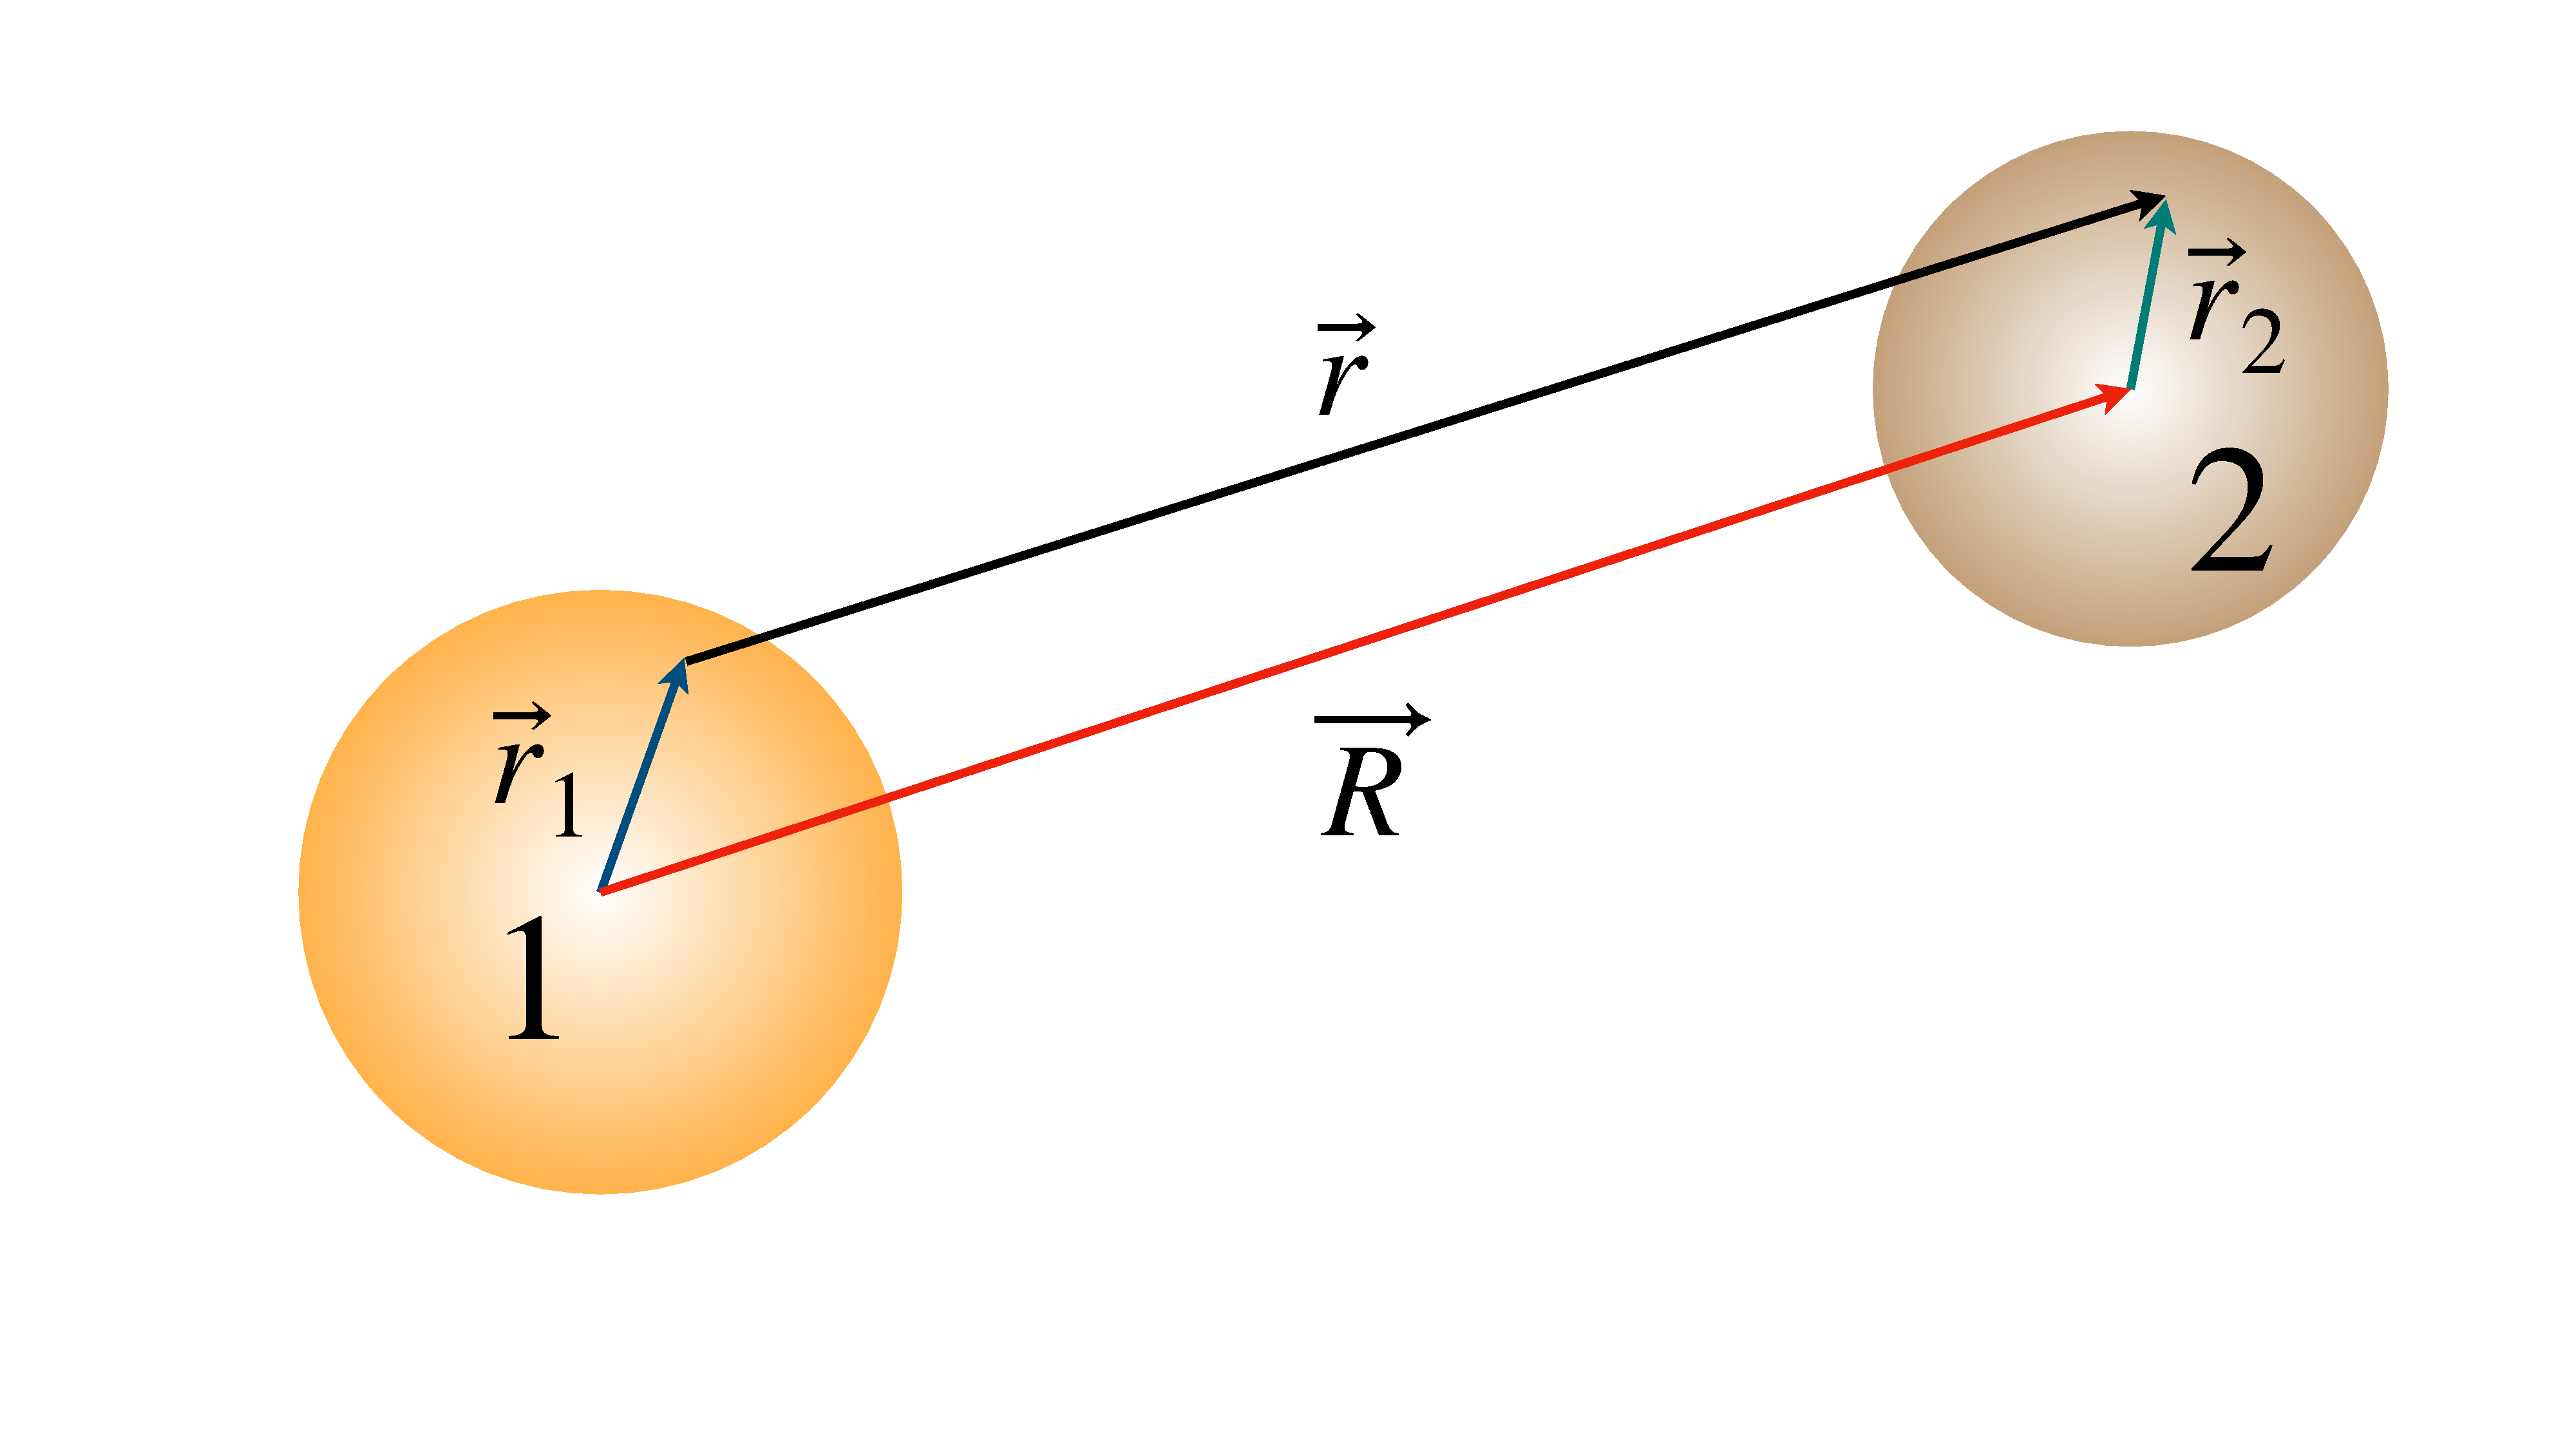
\includegraphics[scale=0.25]{Graphs/DoubleFolding.pdf}
	\caption[Double folding model calculation illustration]{Double folding model calculation illustration. Nuclei, instead of points, are represented as extended structures with finite radii. Then, vector $\vec R$ represents the separation between the center of the nuclei while $\vec r_1$ and $\vec r_2$ are integration variables. }
	\label{fig:DoubleFolding}
\end{figure}


\subsubsection{Calculations with selected NN interactions}

Capture reaction review light nuclei. It included a double folding model with two Yukawa like terms plus additional delta term  for a $NN$ potential given by  \cite{ghasemi_sadeghi_2018}:

\begin{equation}\label{eq:potential_NN_YukawaDelta}
	v(s) = A \frac{\exp {(-\beta_1 s)}}{\beta_1 s} + B \frac{\exp {(-\beta_2 s)}}{\beta_2 s} + C \delta(s),
\end{equation}

with $s = |\vec r + \vec r_2 - \vec r_1|$. Additionally, the spin orbit coupling term is expressed as: 

\begin{equation}\label{eq:potential_M3Y_spinOrbit}
	V_{\mathrm{SO}} = 	- \lambda_{\mathrm{SO}} \left(\frac{\hbar}{m_\pi c}\right)^2 \frac{1}{r} \frac{d}{dr} V(r),
\end{equation}

where $m_\pi$ corresponds to the mass of the pion and $\lambda_{\mathrm{SO}}$ serves as an adjustable parameter for the spin-orbit coupling potential contribution. \\

However, one of the main issues of implementing equation \ref{eq:micro_doubleFolding_potential} is that it involves two three dimensional integration. Alternatively, in order to simplify computations, a Fourier transform may be performed. The convention used for this transformation is given by: 

\begin{equation}\label{eq:micro_doubleFolding_fourierTransform}
	\hat f(\vec k) = \int f(\vec r) \exp(i \hat k \cdot \hat r) d \vec r,
\end{equation}

where the Fourier transform of $f(r)$, as parametrized in the position space, corresponds to the function defined in reciprocal space $\hat f(\vec k)$, with $\vec k$ as parameter. \\

Then, in order to proceed with the transformations, concrete formulae for the densities shall be given. In the case of  $\alpha$ particle, the usual shape is modeled by the function:

\begin{equation}\label{eq:micro_doubleFolding_potential_rhoalpha}
	\rho_\alpha (\vec r_1) = \rho_1 \exp (-\beta r^2_2),
\end{equation}

where $\rho_1$ and $\beta$ are the characteristic amplitude and decay factor of the double exponent like shape. \\

On the other hand, with respect to the core part, a Woods-Saxon term is used. More concretely, the expression: 

\begin{equation}\label{eq:micro_doubleFolding_potential_rhoC}
	\rho_c(\vec r_2) =  \frac{\rho_2}{1 + \exp {\left(\frac{r_1 - r_0}{a'}\right)}},
\end{equation}

with $\rho_2$ as the amplitude and $r_0$ and $a'$ as the radius shift and diffuseness parameters. \\ 

With all these density functions already considered, the computation of $U(r)$ proceeds by applying the inverse Fourier transform to get the transformed potential, in the reciprocal representation, back to the position form. Then, the potential is given by:

\begin{equation}\label{eq:micro_doubleFolding_potential_Fourier}
	U(\vec r ) = \frac{1}{(2\pi)^3} \int { \exp{(-i\hat k \cdot \hat r )} \bar {\rho}_c(\vec k)  \bar {\rho}_\alpha (\vec k) \overline{V_{\mathrm{NN}}}(\vec k)  d\vec k},
\end{equation}

where $\bar {\rho}_\alpha (\vec k)$ and $\bar {\rho}_c(\vec k) $ correspond to the Fourier transforms of the alpha and core densities as well as $\overline{V_{\mathrm{NN}}}(\vec k)$ labels the transformation the $\mathrm{NN}$ potential.  \\

\subsubsection{Clustering}

A double folding potential can be hybridized with clustering for selected reactions. For instance, in the case of $\mathrm{{}^{6}Li + {}^{12}C}$, can be represented as assuming $\mathrm{{}^{12}C}$ as the core interacting with the composed $\alpha + d = \mathrm{{}^{6}Li}$ nucleus as \cite{amer_penionzhkevich_2021}:

\begin{equation}\label{eq:potential_cluster_6Li12C}
	V_{\mathrm{6Li-12C}}(\vec R) = \int \left[V_{\alpha-\mathrm{12C}} \left(\vec R - \frac{1}{3} \vec r\right) + V_{d-\mathrm{12C}}\left(\vec R + \frac{2}{3} \vec r \right) \right]  |\chi_{\alpha d} (\vec r)|^2 d\vec r,
\end{equation} 

where $\chi_{\alpha d}$ corresponds to the inter cluster wave function. Similarly, for the case of $\mathrm{{}^{6}Li + {}^{12}C}$, the potential is given by:


\begin{equation}\label{eq:potential_cluster_6He12C}
	V_{\mathrm{6He-12C}}(\vec R) = \int \left[V_{t-\mathrm{12C}} \left(\vec R - \frac{1}{2} \vec r\right) + V_{t-\mathrm{12C}}\left(\vec R + \frac{1}{2} \vec r\right)  \right] |\chi_{t t} (\vec r)|^2 d\vec r .
\end{equation} 

\subsubsection{Deformed potential}

$\Ofusion$ with  inelastic and elastic scattering description.  and coupled channels based on optical model with folded M3Y NN effective interaction study is presented in \cite{hassanain_al_sebiey_2014}. A deformed potential is introduced by: 

\begin{equation}\label{eq:potential_deformed}
	U^{\mathrm{DP}}_\lambda = - \delta^{U}_\lambda \frac{dU(r)}{dr},
\end{equation} 

with $\delta^{U}_\lambda$ as the deformation length, which is accountable for parametrizing the strength of this potential contribution. Alternatively, the density additional contribution is also obtained similarly with: 

\begin{equation}\label{eq:potential_deformed_density}
	\rho^{\mathrm{tr}}_\lambda = - \delta^{m}_\lambda \frac{d\rho(r)}{dr},
\end{equation} 

where the $\delta^{m}_\lambda$ is usually equivalent to its potential analogous $\delta^{U}_\lambda$, as well it is equal regardless of the kind of nucleon. These densities can be used for calculating folded potentials. \\


\subsubsection{Extended screened potential}

$\mathrm{\ddexchange}$ reaction in metallic environments with screening effect included \cite{czerski_huke_heide_ruprecht_2006}. Screening effect due to electrons damps the Coulomb potential. In a first estimation, the damped $V(r)$ is given by:

\begin{equation}\label{eq:potential_screening_simple}
	V(r) = \frac{e^2}{r} \exp {\left( - \frac{r}{a}\right)},
\end{equation}

with $e$ as the electric charge and $a$ as the diffuseness parameter. A more sophisticated treatment of the screening effect is giving by modeling the Coulomb potential as:

\begin{equation}\label{eq:potential_screening}
	V(r) = \frac{e^2}{r} \Psi(r),
\end{equation}

with $\Psi(r)$ as the correction to be made to the Coulomb potential. An usual approximation to $V(r)$ is given by conveniently evaluating the Fourier transform such:

\begin{equation}\label{eq:potential_screening_fourier}
	V(r) = \frac{1}{(2\pi)^3} \int \frac{4\pi e^2 \phi^2(k)}{\epsilon_\nu (k) \epsilon_c (k) k^2} \exp(i \vec k \cdot \vec r) d^3 \vec k,
\end{equation}

with the form factor $\phi(k)$, being defined with the aid of the Thomas-Fermi approximation, with the form: 

\begin{equation}\label{eq:potential_screening_formFactor}
	\phi(k) = 1 - z + \frac{zk^2}{k^2 + {k'}^2} + \mathcal{O}(z^3),
\end{equation}

where $z$ is an expansion variable and $k'$ is defined as: 

\begin{equation}\label{eq:potential_screening_kThomasFermi}
	{k'}^2 = \frac{6\pi e^2 n}{E_F},
\end{equation}

with $n$ and $E_F$ as the number density and Fermi energy respectively. On the other hand, the dielectric function is given by:

\begin{equation}\label{eq:potential_screening_dielectric}
	\epsilon_\nu = 1 - \frac{\nu(k) P(\nu)}{1 + \nu(k) G(k) P(k)},
\end{equation}

with $\nu(k)$ defined as: 

\begin{equation}\label{eq:potential_screening_nu}
	\nu(k) = \frac{4\pi e^2}{k^2}.
\end{equation}

Additionally, parameters $P(k)$ and $G(k)$ are linked with the polaribizability and electron correlation respectively. Another quantity that is useful for annotating is the polarizability energy $U_{\mathrm{pol}}$, which is defined as: 

\begin{equation}\label{eq:potential_screening_Upolarizability}
	U_{\mathrm{pol}} = \lim_{r \rightarrow 0 } {\left(\frac{e^2}{r} - \frac{e^2}{r} \Phi(r) \right)}.
\end{equation}


\subsection{Non-locality}  \label{sub:potential_nonlocality}

Nuclear interactions are affected by an intrinsic quantum mechanical characteristic in which it is not possible to distinguish the incoming to the out coming particle. For example, if a neutron collides with a nucleus and, as a result of a complex process, it emits another neutron, it is not possible to claim that the exiting neutron is the incoming neutron.  This effect is closely related with the so called Pauli non-locality. \\

\subsubsection{Generalities}

A first approach to model this effect is by considering the action of the potential $V(r)$ when operating the wave function. A general picture of a non-local potential is given by \cite{descouvemont_baye_2010}:

\begin{equation} \label{eq:nonLocality_picture}
	V(r) \psi(r) = U(r) \psi(r) + \int W(r, r') \psi(r') dr'.
\end{equation}

where $\psi(r)$ is related with the wave function, $U(r)$ is the local part of the potential and $W(r, r')$ assumes the role of a kernel term. \\

Notice that the right term involves integration under the primed radius $r'$. This accounts for the fact that non-local potentials are not uniquely defined by the information provided in the point of calculation interest, which is parametrized by $r$ in this case. When the result of equation \ref{eq:nonLocality_picture} is considered, it is possible to conclude that the shape of the Schrödinger will be modified as:

\begin{equation} \label{eq:nonLocality_schrodinger}
	\left(\frac{-\hbar^2 \nabla^2}{2\mu} + V(r)  - E  \right) \psi(\vec r) =   \int W(r, r') \psi(r') dr'.
\end{equation}

This modified form is usually named as the integral Schrödinger equation. When it comes to computing equation \ref{eq:nonLocality_schrodinger}, it would be desired to have an equivalent local potential which gives the same results as the non-local potential. In fact, it is possible to find a matching condition to encounter such effective local potential. The precedent was established by the work on non-local approximations for neutron potentials by Perry and Buck \cite{perey_buck_1962}. They state the connection between non-local $V_{\mathrm{N}}$ and local potentials $V_{\mathrm{L}}$ has the form:

\begin{equation}\label{eq:nonLocality_connection}
	V_{\mathrm{N}} = V_{\mathrm{L}} \exp{\frac{a V_{\mathrm{N}}}{b}}.
\end{equation}

The previous formula gives a way of calculating the desired potential by solving an implicitly defined non-linear equation. For example, a generic potential, which includes Pauli nonlocality, is expressed by \cite{golf_hellmers_weber_2009} by:

\begin{equation}\label{potential_nonLocal_folding}
	V_{\mathrm{F}} = \int \rho_1(\vec r_1) \rho_2(\vec r_2) V_\mathrm{NN} d\vec r_1 d\vec r_2,
\end{equation}

where $V_\mathrm{NN}$ is the nucleon - nucleon potential and $\rho_1(\vec r_1)$ with  $\rho_2(\vec r_2)$ correspond to the pair of densities evaluated at points $\vec r_1$ and $\vec r_2$ respectively. The approximation, which is derived from the Perey and Buck approach, is given by: 

\begin{equation}\label{potential_nonLocal_LE}
	V_\mathrm{LE}(R, E) \approx V_\mathrm{F}(R) \exp [{-\gamma (E - V_C(R) -V_\mathrm{LE}(R, E))}].
\end{equation}

With the gamma defined as:

\begin{equation}\label{potential_nonLocal_b}
	\gamma = \frac{\mu b^2}{2\hbar^2}.
\end{equation}


\subsubsection{São Paulo potential}

This is a classical example of a non-local potential that is widely applied, for example, in alpha-cluster. Reference \cite{bai_ren_2018} has more details. Its form is given by \cite{chamon_2007}:

\begin{equation} \label{eq:potential_SaoPaulo}
	V_{\mathrm{SPP}} (r) = V_{\mathrm{F}} (r)e^{-4V^2/c^2},
\end{equation}

where the velocity like term $V$, is expressed as: 

\begin{equation} \label{eq:potential_SaoPaulo_speed}
	V^2 = \frac{2}{\mu} \left( E - V_{\mathrm{F}}(r) - V_{\mathrm{C}}(r) \right),
\end{equation}

where the reduced mass is $\mu$, the Coulomb potential is $V_{\mathrm{C}}(r)$ and the folded potential  $V_{\mathrm{F}}(r)$. Notice that the fact that $V$ depends on $V_{\mathrm{F}}(r)$, which is used in order to determine $V_{\mathrm{SPP}} (r)$ implies that the potential has to be solved by computing iterations. \\


\subsubsection{Application to alpha decay}

Non-locality review in $\alpha$ decay is given in \cite{rojas-gamboa_velasquez_kelkar_upadhyay_2022}. A WKB quantization condition to be imposed is given by:

\begin{equation}\label{potential_nonLocal_WKB_quantization}
	\int_{r_1}^{r_2} {k(r) dr} = \left (n + \frac{1}{2} \right )\pi,
\end{equation}

where $n$ is an integer that serves to parametrize the quantization. \\

The non-local potential, which could be also referred to as the Mumbai potential, is expressed as \cite{upadhyay_bhagwat_jain_2017}:

\begin{equation}\label{potential_nonLocal_gaussian}
	V_{\mathrm{NL}} (\vec r, \vec r') = \frac{1}{\pi^{3/2}b} U_N \left( \frac{|\vec r + \vec r'|}{2}\right) \exp \left(- \left( \frac{|\vec r - \vec r'|}{2}\right)^2\right),
\end{equation}

with $b$ as the label for the non-locality parameter.\\

Deformed nuclei is given by modifying the Woods-Saxon distribution as by accounting for angle $\theta$ as:


 \begin{equation}\label{potential_nonLocal_modifiedWoodsSaxon}
 	\rho'(r, \theta) = \frac{\rho }{1+\exp{\left(\frac{r-R(\theta)}{a(\theta)}\right)}}.
 \end{equation}
 
The modified parameters are given by:

 \begin{equation}\label{potential_nonLocal_modifiedWoodsSaxon_r}
	R(\theta) = R_0(1 + \beta_2 Y^{2}_{0}(\theta) + \beta_4Y^{4}(\theta)).
\end{equation}

Additionally the diffuseness is corrected with:

 \begin{equation}\label{potential_nonLocal_modifiedWoodsSaxon_a}
	a(\theta) = a'(\theta) \sqrt{1 + |\vec \nabla R(\theta)|^2 }
\end{equation}

with $a'$ being defined as:

 \begin{equation}\label{potential_nonLocal_modifiedWoodsSaxon_aprime}
	a'(\theta) = a_0 \left(1 + \beta_2 Y^{2}_{0}(\theta) + \beta_4Y^{4}(\theta)\right)
\end{equation}

Non-locality assessment in $\alpha$ decay is performed in \cite{perez_velasquez_kelkar_upadhyay_2019}. For the specific case of beta decay, the NN interaction might be modeled as a double Yukawua exponential term like: 

\begin{equation}\label{potential_nonLocal_M3Y}
	V_{\mathrm{NN}}(\vec r_{12}, E) = V_0 \frac{-\beta_0 |\vec r_{12}|}{a_0} - V_1 \frac{-\beta_1 |\vec r_{12}|}{a_1} + J_{00}\delta{\vec r_{12}},
\end{equation}

where $J_{00}$ parametrizes the exchange term of the $\alpha-\alpha$ interaction. The Coulomb potential can also be modified as: 

\begin{equation}\label{potential_nonLocal_coulomb}
	V_{C}(r) = \int \rho^{(C)}_\alpha(\vec r_1) \rho^{(C)}(\vec r_2) \frac{e^2}{|\vec r_{12}|} d\vec r_1 d\vec r_2.
\end{equation}


\subsubsection{Polatization potential}

Coupled channels with optical potential,  polarization potential is studied in \cite{cardenas_canto_donangelo_hussein_lubian_romanelli_2002}. \\ 

An alternative method when treating coupled channel matrix is by constructing a polarization potential, which is defined as: 

\begin{equation}\label{eq:potential_polatization}
	U^{(\mathrm{pol})} = \sum_\alpha {V_{0\alpha} (\vec r) G(E_\alpha, \vec r, \vec r') V_{\alpha0} (\vec r)},
\end{equation}

where the non local $U^{(\mathrm{pol})} $  depends on a local potential $V$ and the Green's function $G(E_\alpha, \vec r, \vec r')$ corresponding to the propagator, which is given by:

\begin{equation}\label{eq:potential_propagator}
	G = \frac{1}{E - QH_0Q + i\epsilon},
\end{equation}

given that $Q = 1 - P$, where $P$ is the projector and $H_0$ is related with the base Hamiltonian. \\

\section{Empirical formulas} \label{sec:empiricalFormulas}

The S-factor energy dependence can be directly estimated by using some conveniently chosen formulas. Unlike the approaches of previous sections, empirical modeling focus on reproducing the form of the S-factor by curve fitting rather than performing cross section computations.

\subsection{Interpolations} \label{sub:empirical_interpolation}

Non-resonant reaction S-factors, which typically have an overall smooth and monotonic behavior, are well suited to polynomial fit calculations. Therefore, the astrophysical S-factor can be estimated as:

\begin{equation}  \label{eq:empirical_polynomial}
	S(E) = a_0 + a_1E + a_2 E^2 + ... a_NE^N \, 
\end{equation}

where coefficients of the form $a_k$ correspond to the weights of the term of order $k$. The sum is interrupted until the maximum exponent $N$, which is named as the order or degree of the polynomial, is reached. Then, based on square error minimization, it is possible to estimate the best value for each coefficient. Additionally, when the order of magnitude of the S-factor curve varies rapidly, there is an useful formula, which is referred to as exponential fit, given by:

\begin{equation} \label{eq:empirical_exponential}
	S(E) = \exp{(g_0 + g_1E + g_2E^2 + g_3E^3 + ... + g_NE^N)}.
\end{equation}

Notice that its form consists of the polynomial expansion indicated in equation \ref{eq:empirical_polynomial} embedded within the exponential term. \\

Interpolations may also arise as accurate approximations to more sophisticated S-factor modeling. For example, in the case of the study of the $\BeRadiativeCapture$ reaction performed by \cite{jennings_karataglidis_shoppa_1998}, the S-factor is initially given by: 

\begin{equation}\label{eq:empirical_sFactor_integralFromula}
	S = C(I^2_0 + 2I^2_2)  \frac{E^3_\gamma (J_{11}\beta^2_{11} + J_{12}\beta^2_{12})}{1 - \exp {(-2\pi \eta(E))}},
\end{equation}

where $E_\gamma = E - E_B$ is the photon energy given in terms of $E$ and $E_\mathrm{B}$, which correspond to the energies of the center of mass and final state of $\mathrm{{}^{8}B}$ respectively. Additionally, $I_0$ and $I_2$ are the radial integrals associated with angular momentum values $l=0$ and $l=2$. The remaining variables are specific to the model, and their particularities are detailed in the aforementioned reference.  \\

A relevant fact used to simplify $S$ is that $I_0$ is quadratic divergent with respect to $E_\gamma$, which means that the integral is given by:

\begin{equation}\label{eq:empirical_sFactor_integralFromula_I.0}
	I_0 \propto \frac{1}{E^2_\gamma}.
\end{equation}

Now, considering that $I_0$ is related to the dominant s-wave contribution, it is concluded that $I_0 \gg I_2$. Consequently, the S-factor can be approximated to a Laurent series by assuming that all the additional terms of equation \ref{eq:empirical_sFactor_integralFromula}, except $E^3_\gamma$, can be Taylor expanded with respect to the photon energy. Therefore, the S-factor is estimated with the formula:

\begin{equation}  \label{eq:empirical_laurent}
	S(E_\gamma) \approx \frac{ a_{-1}}{E_\gamma} + a_0 + a_1 E_\gamma+ a_2 E_\gamma^2 + ... \ .
\end{equation}

It includes a pole at $E_\gamma = 0$ in the specific case studied in the reference. However, for the reactions analyzed in this document, $a_{-1} = 0$, since the S-factor should be smooth at very low energies. Ultimately, this example motivates why the S-factor is described as a Taylor series expansion, as it is shown in equation \ref{eq:empirical_polynomial}. More sophisticated formulas can imply exponential enhancement coefficients due to screening effects. The particularities of these adjustments are presented in section \ref{sub:resultsAnalysisNonResonant}. 

\subsection{Fusion reactions formulas} \label{sub:empirical_fusion}

A formula consistent with the behavior of the S-factor for a  fusion reaction should include the regimes at energies lower and greater than the height of the Coulomb barrier. One possible choice is given by introducing a Woods-Saxon like term in order to distinguish the two aforementioned regions. For example, an empirical formula given in  \cite{beard_afanasjev_chamon_gasques_wiescher_yakovlev_2010} relates the S-factor energy dependence as:

\begin{equation} \label{eq:empirical_yakovlev}
	S(E) = \sum_{k=0}^{N} {a_kE^k} + \left(1 + \exp{\left( \frac{E_c - E}{D}\right)}\right)^{-1} \sum_{l=1}^{M} {b_lE^l},
\end{equation}

where $E_c$ and $D$ are quantities related to the Coulomb barrier and the diffuseness parameter of the Woods-Saxon distribution respectively. \\

In order to check that the formula presented in equation \ref{eq:empirical_yakovlev} is consistent with the expected behavior for fusion reactions, it is essential to be noticed that it gives two different asymptotic behaviors. On the one hand, at the limit of subbarrier energies with $E \rightarrow 0 $, and if $\exp {(E_c/D)} \gg 1$, as it usually happens since $E_c > D$, the right term vanishes and thus the S-factor approaches: 

\begin{equation} \label{eq:empirical_yakovlev_0}
	S(E) \rightarrow \sum_{k=0}^{N} {a_kE^k}. 
\end{equation}

Where the last expression corresponds to a polynomial interpolation of order $N$. On the other hand, for superbarrier energies, at the limit of $E \rightarrow \infty $, the exponential factor leans to $\exp {(-E/D)} \approx 0$ and then the S-factor is expressed as: 

\begin{equation} \label{eq:empirical_yakovlev_infty}
	S(E) \rightarrow \sum_{k=0}^{N} {a_kE^k} + \sum_{l=1}^{M} {b_lE^l}.
\end{equation}

This expression shows that the high-energy behavior corresponds to the low-energy contribution of equation \ref{eq:empirical_yakovlev_0} with an additional polynomial term of degree $M$. Then, the sum of these two polynomials is equivalent to a polynomial of order $\max \{{N, M}\}$. \\

At energies such that $|E_c - E|/D \sim 1$, the S-factor presents a sharp change on its energy dependence due to the transition regime of the Woods-Saxon curve. In particular, a rapid varying transition from the behavior of equation \ref{eq:empirical_yakovlev_0} to equation  \ref{eq:empirical_yakovlev_infty} happens. This break away effect will be visualized in the analysis of fusion reactions in section \ref{sec:nonResonant}. \\

Alternatively, an example of another parametrization which does not depend on Taylor expansions is used in the context of  oxygen-oxygen and oxygen-carbon fusion reactions. It consists of extending the classical hard sphere cross section by including an energy dependent factor. The formula is given by \cite{kovar_geesaman_braid_eisen_henning_ophel_paul_rehm_sanders_sperr_et_1979}:

\begin{equation}\label{eq:middleFusion_empirical_crossSection_Parametrized}
	\sigma_F(E) = \pi R_b^2 \left(1 - \frac{V_b}{E}\right),
\end{equation}

with $R_b$ and $V_b$ are associated with the radius and height of the potential barrier respectively. Particularly, $V_b$ is further parametrized as: 

\begin{equation}\label{eq:middleFusion_empirical_barrier_Parametrized}
	V_b = \frac{Z_1Z_2e^2}{R + a + d},
\end{equation}

where $R = r_0 (A^{1/3}_1 + A^{1/3}_2)$ is the empirical formula for the radius, which is given in terms of the reactant mass numbers $A_1$ and $A_2$, $d$ corresponds to the distance between the surfaces at the barrier and $a$ is model specific term related to the range of the potential. Therefore, the S-factor formula which corresponds to this approach is given by: 

\begin{equation}\label{eq:middleFusion_empirical_sFactor}
	S_F(E) = \pi R_b^2 \left(E - V_b\right) \exp (2\pi \eta).
\end{equation}


\subsection{Resonances and composite formulas} \label{sub:empirical_resonances}


For resonant reactions, the Breit-Wigner formula is the most appropriate approximation for modeling the S-factor shape. An example of a Breit-Wigner fit is given by: 

\begin{equation} \label{eq:empirical_breitWigner}
	S(E) = S_r \frac{\Gamma^2_r/4}{(E-E_r)^2 + (\Gamma_r/2)^2}.
\end{equation}

where the index $r$ runs through all the resonances with total widths and energy peaks being $\Gamma_r$ and $E_r$ respectively. Additionally, a phenomenological parameter for the height of the resonance was included and is named as $S_0$. \\

 Note that this is a modification of equation \ref{eq:rmatrix_breitWigner} when $\gamma = \Gamma/2$, which is consistent with interpreting $\Gamma$ as the double of the two partial widths $\gamma$. Additionally, the resonance amplitude has a relation with the cross section value, based on the Breit-Wigner formula, which can be expressed, for the case of $l = 0$, as: 
 
 \begin{equation} \label{eq:empirical_breitWigner_S0}
 	S_0 \sim  \frac{\pi}{k^2}. 
 \end{equation}

This formulation permits empirical formulas to add resonant terms to the non-resonant estimation. Usually, the resonant terms are added to a background which is fitted to a non-resonant formula. For example, consider the expression: 

\begin{equation}  \label{eq:empirical_hybridPolynomial}
	S(E) =  \sum _{k = 0}^{N} {a_kE^k} + \sum_{l = 1}^{M} {\frac{c_l}{(E - E_l)^2 + \Gamma_l^2/4}},
\end{equation}

where $c$ is a parameter with units of those of the width squared. When comparing the last formula with equation \ref{eq:empirical_breitWigner}, it happens that $c_l = \Gamma^2_l/4$ is the best estimation. \\

Analogously, if the non-resonant term has a polynomial form, the S-factor is expressed as:

\begin{equation}  \label{eq:empirical_hybridExponential}
	S(E) =  \exp { \left( \sum _{k = 0}^{N} {a_kE^k} \right) } + \sum_{l = 1}^{M} {\frac{\Gamma_l^2/4}{(E - E_l)^2 + \Gamma_l^2/4}},
\end{equation}

where $N$ is the order of the polynomial which estimates the non-resonant background and $M$ represents the number of resonances considered.  \\

\chapter{S-factor calculations for selected reactions} \label{ch:sfactorCalculations}

Astrophysical S-factor calculations for a selected list of reactions will be presented. The list distinguishes between resonant and non-resonant reactions. Additionally, various astrophysical environments like Big Bang Nucleosynthesis, pp-chain, CNO cycle and middle heavy nuclei fusion are included.  \\

Selected reactions calculations are based on specific models conveniently chosen to reproduce the S-factor behavior. Particularly, since most of microscopical and R-matrix treatments require sophisticated parametrizations and imply considerable computational resources, potential models and empirical formulas are preferred as a first approximation for S-factor calculations in this work.  \\

Potential models and empirical formulas typically include free parameters. The values of these parameters are fitted to experimental data in order to obtain the error minimizing prediction. Consequently, S-factor experimental data gathering is of special concern in this work. In order to account for this need, several experimental data sources were consulted. Most of these references were extracted from databases like NACRE II \cite{xu_takahashi_goriely_arnould_ohta_utsunomiya_2013}. Further related details are given in Appendix \ref{ap:literatureData}. \\ 

With experimental data given, fitting of the S-factor values of the selected reaction follows. Details corresponding to fitting procedures are covered in Appendix \ref{ap:fitting}.  In particular, the values of the fitting parameters determined in this work are presented in Section \ref{sec:empiricalFitting}.  \\

In order to perform the numerical computations for fits, a set of programs were written as specified in Appendix \ref{ap:codes}. The programming language used was Python \cite{rossum_drake_2009}. In addition, data management depended on Pandas \cite{mckinney_2010}, numerical computations were performed on top of subroutines from NumPy  \cite{harris_millman_vanderwalt_gommers_virtanen_cournapeau_wieser_taylor_berg_smith_et_2020}, fitting parameters were obtained with SciPy \cite{virtanen_gommers_oliphant_haberland_reddy_cournapeau_burovski_peterson_weckesser_bright_et_2020} and data was visualized with the support of Matplotlib \cite{hunter_2007}. \\

The evaluation of the models to be studied in this chapter is divided in two main parts: non-resonant and resonant reactions.  In addition, for each subsection of the chapter, calculations considerations are included. Subsequently, the results and analysis of the S-factor calculation for each  selected reaction are presented.

\section{Non-resonant reactions} \label{sec:nonResonant}

The results produced by this work start with the study of the background of the S-factor energy curves for the selected reactions. In particular, most of the backgrounds of reactions are modeled as having non-resonant behavior. Then, the study of non-resonant reactions has priority as a first approximation to the calculation of the astrophysical S-factor. \\

The selected non-resonant reactions include light heavy nuclei exchange reaction $\mathrm{{}^{2}{H}(d,p){}^{3}{H}} $ and radiative capture reaction  $\mathrm{{}^{2}{H} (p, \gamma) {}^{3}{He}} $. The first reaction is critical for Big Bang Nucleosynthesis since it provides a way of fusing deuterium, which is essential for the production of heavier nuclei in the early universe \cite{coc_vangioni_2010}. The second reaction is a pivotal process in the pp-chain as it produces $\mathrm{{}^{3}He}$, which is a prerequisite  for producing the ending product of the chain $\mathrm{{}^{4}He}$ \cite{fowler_1958}. \\

 On the other hand, the middle heavy nuclei fusion reactions to be considered contain carbon and oxygen isotopes as reactants. These types of reactions are considered since the low-energy study of these two reactions are of recent research interest \cite{torilov_maltsev_zherebchevsky_2021, taniguchi_kimura_2021,mukhamedzhanov_pang_kadyrov_2019}. In fact, new successful models usually include aspects inherent on middle heavy nuclei like clustering \cite{assuncao_descouvemont_2016} or couplings to vibrational modes \cite{duarte_gasques_oliveira_zagatto_chamon_medina_added_seale_alcantara-nunez_rossi_et_2015}. \\
 
 Particularly, the $\Cfusion$  and $\Ofusion$ reactions are selected since they are essential for the burning process in massive stars at the end period of their lives. Additionally, the $\mathrm{{}^{12}C + {}^{16}O}$ reaction is also chosen due to the relevance of the study of the fusion of the two more stable carbon and oxygen nuclei. Lastly, other oxygen fusion channels like $\mathrm{{}^{16}O + {}^{17}O}$ and $\mathrm{{}^{16}O + {}^{18}O}$ are selected given their close relation to the $\Ofusion$ reaction, as well due to the existence of inelastic contributions corresponding to excited $\mathrm{O^{17*}}$ and $\mathrm{O^{18*}}$ nuclei \cite{thomas_chen_hinds_meredith_olson_1986}.   \\

 
\subsection{Calculation considerations} \label{sub:considerationsNonResonant}

Empirical formulas are initially considered for the light heavy S-factor description. In particular, the non-resonant part of the equations \ref{eq:empirical_hybridExponential}  and \ref{eq:empirical_hybridPolynomial} are fitted to experimental data.  \\

Fitting parameters to best describe experimental data were determined for empirical formulas. In particular, the parameters chosen minimized the chi-squared $\chi^2$ function as it is described in appendix \ref{ap:fitting}. In some cases, it was necessary to constraint the interval of validity of the parameters in order to avoid unphysical behavior of the fittings. Further details about these constraints can be found in section \ref{sec:empiricalFitting}. \\

On the other hand, fusion reactions are described by the Yakovlev et. al empirical formula \cite{beard_afanasjev_chamon_gasques_wiescher_yakovlev_2010} and analytical potential model  \cite{yakovlev_beard_gasques_wiescher_2010}.  \\

Particularly, in the Yakovlev model, parameters are fitted as follows: The initial free parameters are $\delta$, $E_c$,  $\xi$ and $S_0$, which parametrize the nuclear-electromagnetic transition of the potential, the Coulomb barrier, the asymptotic value of the S-factor at higher energies and the low energy extrapolation of the S-factor respectively.  \\

Then, additional parameters are introduced in order to take into account the atomic and massive numbers of the colliding nuclei. For example, the Coulomb barrier like term is given in terms of a new parameter $R$ as follows:

\begin{equation} \label{eq:potential_Yakovlev_Ec}
	E_c = \frac{\alpha}{R},
\end{equation}

where $\alpha = \sqrt{Z_1Z_2e^2}$ and $R$ is determined in terms of the mass numbers $A_1$ and $A_2$ as well as the atomic numbers $Z_1$ and $Z_2$ of the reacting nuclei as:

\begin{equation} \label{eq:potential_Yakovlev_R}
	R = R_0 + \Delta R_{1} |2Z_1 - A_1| + \Delta R_{2}|2Z_2 - A_2|.
\end{equation}

In particular, the parameter $R_0$ is unique for a given combination of $Z_1$ and $Z_2$ values,  the parameters $\Delta R_{1}$ and $\Delta R_{2}$ are specific for each reactant nuclei. In addition, this parameter takes different values given in the following way: 

\begin{equation} \label{eq:potential_Yakovlev_R1}
	\Delta R_1= 	\left\{\begin{array}{l}
		\begin{split}
			\Delta R_{10}, \quad & 2Z_1 \ge A_1.\\ 
			\Delta R_{11}, \quad & 2Z_1 < A_1.
		\end{split}
	\end{array}\right.
\end{equation}

Analogously, $\Delta R_2$ is determined as: 

\begin{equation} \label{eq:potential_Yakovlev_R2}
	\Delta R_2= 	\left\{\begin{array}{l}
		\begin{split}
			\Delta R_{20}, \quad & 2Z_2 \ge A_2.\\ 
			\Delta R_{21}, \quad & 2Z_2 < A_2.
		\end{split}
	\end{array}\right.
\end{equation}

In quite a similar manner, the $\xi$ parameter is expressed in terms of two new parameters $\xi_0$ and $\xi_1$ with the form:

\begin{equation} \label{eq:potential_Yakovlev_xi}
	\xi = 	\xi_0 + \xi_1(A_1 + A_2).
\end{equation}

Then, $\xi_0$ can be interpreted as a zero order approximation for $\xi$ while $\xi_1$ is the correction term coupled to the total mass number of the reacting nuclei. The numerical values of the 9 lastly mentioned parameters are provided in the Table II contained in \cite{yakovlev_beard_gasques_wiescher_2010}. \\

Finally, although Yakovlev et al. model is used for middle-heavy fusion reactions, it is not expected to work for radiative capture reactions since it predicts a decrement of the S-factor for all energies. In contrast, the S-factor increases in radiative capture reactions.  \\

Actually, for calculations, data from the modified astrophysical S-factor $S^{*}$ is usually given instead of unmodified S-factor data. The expression of this new factor is given by:

\begin{equation}\label{eq:potential_modifed_Sfactor}
	S^{*}(E) = S(E) \exp {(g_1E)},
\end{equation}

where the constant is widely chosen to be $g_1 = 0.46 \mathrm{MeV^{-1}}$. Then, experimental points were chosen by computing $S(E)$ values with the expression of equation \ref{eq:potential_modifed_Sfactor} and with experimental data for $S^{*}(E)$.


\subsection{Results and analysis} \label{sub:resultsAnalysisNonResonant}

Results are given in this section regarding the $\ddexchange$ reaction as presented in Figure \ref{fig:2H(d,p)3H}. Initially, polynomial interpolations were calculated with orders $N = 1$ to $N = 5$ as it is visualized in Figure \ref{sfig:2H(d,p)3H-poly12345}. The generality of these fits is that the greater the polynomial order, the better the fit. In particular, the best is obtained with a polynomial of order $N = 5$.  \\

Similarly, exponential interpolations were obtained with $N$ ranging from 1 to 5. These fits are visualized in Figure \ref{sfig:2H(d,p)3H-exp12345}. Additionally, as it happens with polynomial fits, the best fit is given with $N = 5$. However, the polynomial fitting approach gives a better result than this exponential treatment. \\

In particular, this difference could be attributed to the fact that exponential fitting is more ideal when the order of magnitude varies considerably. Therefore, since the S-factor values have all roughly the same order of magnitude, the fitting capacity of the exponential function is limited. In addition, given that exponential fit leans to reproduce data with higher S-factor values, which happens because choosing to fitting better these data points will minimize the square error, the low energy entries are more sensible to errors.  \\

Additionally, it is observed that fits slightly overestimate the reaction S-factor at the lower energies of the plot. This deviation is due to the fact that values from RA02 data principally, as well as GR95 data in a minor extent, are pushing the S-factor estimations up. This S-factor increase is attributed to enhancements caused by the screening effect. A treatment of this S-factor increase is going to be treated in a moment. \\

 In fact, it is noticeable that very low energy values for the S-factor are not entirely consistent since various experiments give noticeable different values for points with similar energy. Then, an additional fifth order fit called poly5-exclude was calculated by not including disruptive data, in which are included RA02 and GR95. This fit is visualized, with polynomial and exponential order five fits, in the best fit graph given in Figure \ref{sfig:2H(d,p)3H-exp5-poly5-best}.

\graphWrapper{
	\subGraph{2H(d,p)3H-poly12345}{Polynomial fits.}
	\subGraph{2H(d,p)3H-exp12345}{Exponential fits.}
	\subGraph{2H(d,p)3H-exp5-poly5-best}{Best fits.}[1]
}
{2H(d,p)3H}{Polynomial and exponential fits $\ddexchange$ reaction}{Empirical formulas fitted to $\ddexchange$ reaction S-factor data. In panel a), poly1, poly2, poly3, poly4, and poly5 represent fits to polynomials from 1st to 5th order.  Similarly, in panel b), exp1, exp2, exp3, exp4 and exp5 represent exponential fits up to 5th order. Additionally, in panel c), poly5-exclude corresponds to a poly5 fit without data from RA02 and GR95. References to the sources of the black colored experimental points are given in Table \ref{table:light_nonResonant}. Fitting parameters values are given in Tables \ref{table:fitting_empirical_dd_poly} and \ref{table:fitting_empirical_dd_exp}.}


Now, resuming the screening effect considerations, at low-energies as far as $ \mathrm{10^{-3} \ MeV}  <  E<\mathrm{10^{-2} \ MeV}$, an exponential-like damping of the S-factor is observed. In fact, this behavior could be explained due to the electron screening effect \cite{raiola_migliardi_gyurky_aliotta_formicola_bonetti_broggini_campajola_corvisiero_costantini_et_2002}. In particular, the enhancement factor $f$ for the S-factor is defined as \cite{assenbaum_langanke_rolfs_1987}: 

\begin{equation}\label{eq:screening_factor}
	f = \frac{E}{E + U_e}\exp{\left(\frac{\pi \eta U_e}{E}\right)},
\end{equation}

where $E$ is the center of mass energy, $\eta$ is the Sommerfeld parameter and $U_e$ is a parameter that quantifies the degree of enhancement of the S-factor. The sharp increase of the S-factor at low energies is explained by the shielding of the Coulomb potential produced by the electron cloud that surrounds the interacting nuclei \cite{assenbaum_langanke_rolfs_1987}. In particular, this dismissal of the strength of the potential reduces the Coulomb barrier. Therefore, as the tunneling probability increases, the cross-section, and thus the S-factor, of the reaction also increases. \\

Additionally, the value of the $U_e$ parameter is usually obtained by fitting. An example of such fitting is found in the graphs of Figure \ref{fig:2H(d,p)3H-screening-exp5-poly5-exclude}.

\graph{2H(d,p)3H-screening-exp5-poly5-exclude}{Screening effect $\ddexchange$ reaction}{Polynomial fits to experimental data with screening effect. The curve labeled as screening-all-fit is obtained by fitting $U_e$ with all data points, screening-only-RA02-fit is obtained only with RA02 data,  \textit{screening-Ue-theory} is calculated with $U_e$ fixed to the value given in RA02. The poly5-exclude fit of Figure \ref{fig:2H(d,p)3H} was used as the S-factor estimation without screening of the last three curves. Additionally, the screening-RAO2 curve presents the S-factor prediction made in the RA02 paper. Further details about the fitting parameters and their values are given in Table \ref{table:fitting_empirical_dd_screening}.}

Initially, the RA02 calculation \cite{raiola_migliardi_gyurky_aliotta_formicola_bonetti_broggini_campajola_corvisiero_costantini_et_2002} was tested against data. This estimation is referred as RAO2-paper in the last plot. Despite the fact that this prediction is able to accurately reproduce the S-factor values of their measurements, namely those marked with the RA02 tag, it is unable to fit appropriately points with higher energies than 0.1MeV. Then, a more comprehensive fitting was needed to be introduced. \\

In response to this improvement need, the poly5-exclude curve for background estimation calculated in this work was used. Then, in order to account for the screening data, the enhancement factor given in equation \ref{eq:screening_factor} was multiplied to the background estimation. In a first approach, a fitting with all data was made, which is visualized with the label screening-all-fit. However, since the S-factor prediction for the RA02 entries were improvable, a second curve was determined by only taking into account RA02 data, which is given the name of screening-only-RA02-fit. In this case, the fit appropriately fits both the screening affected RA02 data and the remaining  background. Therefore, this result can be regarded as an improvement for the RA02 calculation. \\

Finally, as it is visualized in the curve labeled as screening-Ue-theory, the S-factor background estimation calculated in this work also approximates acceptably the S-factor values with the value of the $U_e$ parameter given in the RA02 paper \cite{raiola_migliardi_gyurky_aliotta_formicola_bonetti_broggini_campajola_corvisiero_costantini_et_2002}. In particular, details regarding the determination of this parameter are encountered in Table \ref{table:fitting_empirical_dd_screening}. \\

The analysis now proceeds with the study of the S-factor curves related to the $\dRadiativeCapture$ presented in Figure \ref{fig:2H(p,gamma)3He}. This reaction was treated similarly than previous since there are polynomial and exponential fits. However, there is not a considerable screening effect caused S-factor enhancement. \\

Firstly, polynomial interpolations fits were determined. The result of this fitting is visualized in Figure \ref{sfig:2H(p,gamma)3He-poly12345-bounds}. As it happened with the polynomial fits related to the $\ddexchange$ reaction, there is a general tendency of S-factor estimation improvement with the increase of polynomial order. However, in this case the best fit occurred with $N = 4$, not with $N = 5$. \\

A possible cause of this finding can be associated with parameter overestimation. In addition, it is essential to comment that it was not possible to obtain fitting parameters without constraints, which eventually affected the least-squares optimization process. Then, it was likely that the polynomial with $N = 4$ had the necessary parameters to reproduce the S-factor results but also the sufficient number of them to not overestimate the selection of data with higher energies, as it happens with the $N = 5$ interpolation. \\

Secondly, exponential fits were calculated with results visible in Figure \ref{sfig:2H(p,gamma)3He-exp12345}. Fits approximate better to S-factor values with greater $N$. However,  in the $\dRadiativeCapture$ case, the fits do not entirely converge for low energy values. In particular, it seems that the fitting process is choosing the higher S-factor values rather than lower values for error minimizing. Then, it is more complex to this empirical formula to account for low energy data. This reasoning is similar to those made when commenting the exponential fits of the $\ddexchange$ reaction. \\

Lastly, selected fits are zoomed in as it is shown in Figure \ref{sfig:2H(p,gamma)3He-selected-exp5-poly45}. Given the comparison of the fits, it follows that the most robust is given by the fourth order polynomial interpolation.


\graphWrapper{
	\subGraph{2H(p,gamma)3He-poly12345-bounds}{Polynomial fits with constraints.}
	\subGraph{2H(p,gamma)3He-exp12345}{Exponential fits.}
	\subGraph{2H(p,gamma)3He-selected-exp5-poly45}{Selected fits.}[1]
}
{2H(p,gamma)3He}{Polynomial and exponential fits $\dRadiativeCapture$ reaction}{Empirical formulas fitted to the S-factor for the $\dRadiativeCapture$ reaction. In panels a) and b) polynomial and exponential fits up to fifth order are presented respectively.  In particular, the fit parameters used for the graphs in panel a) were constrained. Additionally, in panel c), the best selected fits are visualized. The references to the experimental points are given in Table \ref{table:light_nonResonant}. The values of the fitting parameters are encountered in Tables \ref{table:fitting_empirical_dp_poly} and \ref{table:fitting_empirical_dp_exp}.}


With respect to middle heavy nuclei fusion reactions, the Yakovlev et al. model of \cite{yakovlev_beard_gasques_wiescher_2010} is considered as the analytical model. In addition, Beard and collaborators, in whom Yakovlev is included, present an empirical formula useful to reproduce middle heavy fusion behavior \cite{beard_afanasjev_chamon_gasques_wiescher_yakovlev_2010} is also used. \\

In this work, fits are done based on the previous empirical formula  with the advantage that parameters are determined by fitting data points directly. In contrast, both of the referenced approaches attempt to estimate São Paulo potential model calculations which are not necessarily close to actual experimental data, specially at energies below the Coulomb barrier. \\

As a starting point, S-factor estimations for the $\Cfusion$ reaction are presented in Figure \ref{fig:12C12C} using the potential and empirical Yakovlev estimations, as well as empirical fits to equation \ref{eq:empirical_yakovlev} with $N = 3$ and $M = 2$. In addition, data survey for this reaction was concentrated at energies below the Coulomb barrier given that both of the cited models were already tested successfully at energies above the barrier against experimental data.

\graph{12C12C}{Potential model prediction $\mathrm{{}^{12}C + {}^{12}C}$ reaction }{Astrophysical S-factor prediction for the $\Cfusion$ reaction as parametrized in the Yakovlev et al. analytical potential model \cite{yakovlev_beard_gasques_wiescher_2010}. In addition, two empirical fittings are included. References for experimental points are presented in Table \ref{table:fusion}. Parameters related to empirical fits are given in Table \ref{table:fitting_empirical_12C12C}.}

It is observed that both the potential and empirical external calculations underestimate the value of S-factor. Meanwhile, the plot calculated from this work passes through most data points. This distinction is not exclusive to the $\Cfusion$ reaction. In fact, this is a pattern present in more middle heavy fusion reactions. \\

Additionally, one of the key features of the $\Cfusion$ channel is the presence of various low-energy resonances \cite{notani_esbensen_fang_bucher_davies_jiang_lamm_lin_ma_martin_et_2012}. In fact, this resonant behavior seems to be out of the scope of the Yakovlev potential predicting capacity, as well certainly far from being taken into account with the empirical formula used.  Therefore, further predictions should be able to parametrize these resonances and to give a more accurate S-factor estimation with composite non-resonant and resonant contributions. \\

In fact, the $\mathrm{{}^{12}C + {}^{16}O}$ reaction also presents resonant peaks at energies below the Coulomb barrier, as it is seen in Figure \ref{fig:12C16O} and as it is reported in literature \cite{torilov_maltsev_zherebchevsky_2021}. As it happens with the $\Cfusion$ reaction, this work fit passes through most of the experimental points up to a certain energy, when there is a deviation from the main behavior of the S-factor data. In contrast, both of the Yakovlev et al. estimations underestimate the S-factor values at low energies but predict closely values at higher energies. \\

\graph{12C16O}{Potential model prediction $\mathrm{{}^{12}C + {}^{16}O}$ reaction }{Astrophysical S-factor prediction for the $\mathrm{{}^{12}C + {}^{16}O}$ reaction as parametrized in the Yakovlev et. al analytical potential model \cite{yakovlev_beard_gasques_wiescher_2010}. Additionally,  two empirical fittings are included. The reference for the experimental points is given in Table \ref{table:fusion}. The values of the empirical fits parameters are given in Table \ref{table:fitting_empirical_12C16O}.}

This difference might be explained by considering that the fittings presented in work are minimizing error by usually choosing to fit more appropriately values with higher S-factor. This bias could sufficiently explain why the accuracy of S-factor calculations decreases at energies above the Coulomb barrier. On the other hand, discrepancies between the predictions of the cited models and data are produced since they do not account for aspects inherent to the microscopical behavior of middle heavy nuclei like carbon and oxygen  \cite{duarte_gasques_oliveira_zagatto_chamon_medina_added_seale_alcantara-nunez_rossi_et_2015}. \\

In particular,  since Yakovlev et al. calculations are based in barrier penetration models like the São Paulo model reported in \cite{yakovlev_beard_gasques_wiescher_2010} which does not account for nuclei substructures, it underestimates the fusion cross section since this approach does not include details on the nuclei like coupling with inelastic states or the existence of screening effect S-factor enhancement \cite{koyuncu_soylu_2018}. \\

In a similar way, the S-factor of oxygen fusion reactions of Figure \ref{fig:Oreactions} present low-energy differences in the prediction at low energies for the referred Yakovlev et al. calculations. Then, the empirical fitting proposed in this work serves as an improvement for low energy data extrapolation. \\

With respect to the results related to the $\Ofusion[16][18]$ reaction as presented in Figure \ref{sfig:16O16O}, it is observed how the fit calculated in this work estimates appropriately the S-factor for the complete range of energies of the graph. On the other hand, as anticipated, the cited models underestimate the S-factor at energies below the Coulomb barrier. \\

Similarly, the S-factor values related to the $\Ofusion[16][17]$ reaction illustrated in Figure  \ref{sfig:16O17O} shares a similar behavior as compared to the previous reaction. However, there were not available calculations for the Beard et al. empirical formula. Additionally, both of the fits were less accurate than those presented for the $\Ofusion[16][18]$ reaction analysis. This difference might be caused because of inherent aspects of the $\mathrm{{}^{17}O}$ nuclei. In particular, it is known of the existence of inelastic channels related to both $\mathrm{{}^{17}O}$ and $\mathrm{{}^{18}O}$ nuclei \cite{kovar_geesaman_braid_eisen_henning_ophel_paul_rehm_sanders_sperr_et_1979}. Moreover, the fact that $\mathrm{{}^{17}O}$ has an even $A$ number could introduce more instability and potentially higher fusion capacity. \\

Finally,  $\Ofusion$ data is visualized in Figure \ref{sfig:16O18O}. As it happened to the last two reactions, the values corresponding to the S-factor are fitted better at energies below the Coulomb barrier with the empirical fit determined in this work and at energies above the barrier with the Yakovlev and collaborators potential model and empirical formula. Particularly, an entry with theoretical perdition with São Paulo data was included in order to illustrate the closeness of the cited papers results to this theoretical calculation. 


\graphWrapper{
	\subGraph{16O18O}{$\Ofusion[16][18]$ reaction.}
	\subGraph{16O17O}{$\Ofusion[16][17]$ reaction.}
	\subGraph{16O16O}{$\Ofusion[16][16]$ reaction.}[1]
}
{Oreactions}{Potential model prediction for a selection of oxygen fusion reactions.}{Potential model prediction for a selection of oxygen fusion reactions. In panels a), b) and c) are presented the  Yakovlev et al. prediction for the S-factor, as well as empirical two empirical fittings,  of the $\Ofusion[16][18]$, $\Ofusion[16][17]$ and $\Ofusion$ reactions respectively. Additionally, in panel c), the \textit{SaoPaulo} entry corresponds with the predictions made in \cite{yakovlev_beard_gasques_wiescher_2010} which were obtained by using the São Paulo potential model. Experimental data sources are cited in Table \ref{table:fusion}. Values of empirical fits parameters are given in Tables \ref{table:fitting_empirical_16O18O}, \ref{table:fitting_empirical_16O17O} and \ref{table:fitting_empirical_16O16O}.}


\section{Resonant reactions} \label{sec:resonant}

It is frequent to find sharp peaks in the S-factor values of some nuclear reactions. The existence of these fluctuations usually suggests the presence of resonant phenomena, which cannot be explained effectively with only background estimation. \\

In this work, the radiative capture $\mathrm{{}^{7}{Be}(p, \gamma){}^{8}{B} } $ and $\mathrm{{}^{13}{C}(p, \gamma){}^{14}{N}} $ reactions were selected. The first has astrophysical relevance since it produces a tripe-alpha nuclei like $\mathrm{{}^{8}B}$ \cite{coc_2012}. The second is essential in the CNO and hot CNO cycles \cite{wiescher_gorres_schatz_1999}. \\

A first approach towards the description of resonances consists of introducing a Breit-Wigner (BW) term in the S-factor calculation. In particular, the most simple estimation is provided by assuming that the reaction proceeds with a single channel. Then, the astrophysical S-factor can be approximated as the expression given in equation \ref{eq:rmatrix_sfactor}. \\

In particular, each peak is characterized by additional variables like its height, width and energy center, referred to as $S_0$, $\Gamma_r$ and $E_r$ respectively. With these new variables taken into account, the non-resonant astrophysical S-factor predictions of section \ref{sec:nonResonant} shall be modified.\\

Usually, more sophisticated treatments of resonances require more advanced approaches than bare curve fitting. For instance, the S-factor values of several radiative capture reactions can be analyzed by using the R-matrix model \cite{descouvemont_adahchour_angulo_coc_vangioni-flam_2004}. The main advantage of this approach is that resonances are intuitively included by adding parameters to the model.

\subsection{Calculation considerations} \label{sub:considerationsResonant}

The Breit-Wigner empirical formula is used for empirical fitting of the resonant part. However, not all the regions of S-factor energy curve for a reaction with resonances are going to coincide with resonant behavior. In contrast, these regions are critical in order to estimate the non-resonant background of the reaction.\\

For the purpose of this work, there are two methods for background estimation. The first method consists of fitting a polynomial or exponential function to data including the whole dataset. This is specially convenient when resonances are narrow as compared to the total energy range, like it happens in the $\BeRadiativeCapture$ reaction.  \\

On the other hand, when a resonance occupies almost all the energy range, it is better to fit the Breit-Wigner function first. Then, residuals, which represent the differences between predictions and experimental values, are calculated. Ultimately, the background estimation is given by fitting the remaining residuals of the fit. An example of this approach is given in the study of the $\CRadiativeCapture$ reaction. In both cases, the total S-factor is computed by summing the resonant and non-resonant contributions. This sum is consistent since the S-factor is proportional to the cross section, which is an additive quantity. \\

Finally, in the special case of estimating the background of the reactions with polynomial functions, it is usually convenient to modify slightly the Breit-Wigner fitting function. In particular, an extra parameter $c$ related to the width is included. Then, the resonant contribution of equation \ref{eq:rmatrix_sfactor} is substituted with the expression \cite{sparta_pizzone_bertulani_hou_lamia_tumino_2020}:

\begin{equation}\label{eq:rmatrix_sfactor_modified}
	S(E) = S_0 \frac{c_r}{(E - E_r)^2 + \Gamma_r^2/4}. 
\end{equation}

\subsection{Results and analysis} \label{sub:resultsAnalysisResonant}

Estimation for background and resonant contributions for the $\BeRadiativeCapture$ reaction are visualized in Figure \ref{fig:7Be(p,gamma)8B-parts}. In particular, in Figures \ref{sfig:7Be(p,gamma)8B-poly} and \ref{sfig:7Be(p,gamma)8B-exp} the polynomial and exponential background estimations, which were calculated in this work, are illustrated. Notice that, in contrast to the correlation between fitting quality and order number reported in section \ref{sub:resultsAnalysisNonResonant}, fits with higher order present a nonphysical behavior at higher energies. In fact, the best fits are those with $N = 1, 2$.  \\

This difference can be also contrasted in the high values of most the errors of the parameters as $N$ increases, as it is shown in Tables \ref{table:fitting_empirical_BeRadiative_exp} and \ref{table:fitting_empirical_BeRadiative_poly}. In particular, the curves with $N = 4$ for both exponential and polynomial formulas were too deviated from S-factor data that the fitting algorithm was unable to determine errors for the parameters.   \\

This finding could be explained by considering the effect of parameter overdetermination. In particular, since low order fits are ideal enough, a further increment in the degrees of freedom of the fitting function will cause conflicts between already well determined parameters and new parameters, which have a higher contribution at larger energies. Therefore, for the sake of simplicity, the selected background estimations for the $\BeRadiativeCapture$ reaction are those related with $N = 1$ order fitting formulas as it is visualized in Figure \ref{sfig:7Be(p,gamma)8B-BW-exp1-poly1}. \\

Actually, a fine splitting is observed between the exponential and polynomial fits. In particular, the exponential contribution presents slightly higher values than those calculated from the polynomial contribution. Although at this range of energies this discrepancy might not be considered as substantial, this could be of interest when extrapolating S-factor data to larger energies. In particular, it seems more plausible that the exponential fit would extrapolate better than the polynomial fit when considering the SC06 entry point at $E \approx$ 3.0MeV. \\

\graphWrapper{
	\subGraph{7Be(p,gamma)8B-poly}{Polynomial fits.}
	\subGraph{7Be(p,gamma)8B-exp}{Exponential fits.}
	\subGraph{7Be(p,gamma)8B-BW-exp1-poly1}{Selected fits.}[1]
}
{7Be(p,gamma)8B-parts}{Background and resonance fits for the $\BeRadiativeCapture$ reaction}{Empirical formulas fitted to background of the S-factor for the $\BeRadiativeCapture$ reaction. In panels a) and b) polynomial and exponential fits up to sixth order are presented respectively. Additionally, in panel c), the most simple and accurate fits, in this case exp1 and poly1, were selected. In addition, the BW labeled curve corresponds to a Breit-Wigner fit for the resonance.  The references to the experimental points are given in Table \ref{table:light_resonant}. The values of the fitting parameters are found in Tables \ref{table:fitting_empirical_BeRadiative_poly}, \ref{table:fitting_empirical_BeRadiative_exp} and  \ref{table:fitting_empirical_BeRadiative_BW}.}



\graph{7Be(p,gamma)8B-background-exp1-poly1}{Joint resonant and non-resonant fit for the $\BeRadiativeCapture$ reaction}{Empirical fit for the $\BeRadiativeCapture$ reaction. In this graph, the resonant contribution, as modeled with a Breit-Wigner formula, was added to the non-resonant background estimation, which was modeled with first order polynomial and exponential formulas. In addition, fitting parameters are found in Table \ref{table:fitting_empirical_BeRadiative_composite}.}


A single resonance with a peak close to $E \approx$ 0.7 MeV is observed in Figure \ref{fig:7Be(p,gamma)8B-background-exp1-poly1}. Then, in order to describe the single resonance, a Breit-Wigner fit was performed. In particular, the fitting parameters are given in Table \ref{table:fitting_empirical_BeRadiative_BW}. However, as it is visualized in S-factor dependence, this fit does not account for the entire behavior of the experimental points far from the resonance. Consequently, there is the need of including the non-resonant part which was previously calculated. \\

Lastly, with both resonant and non-resonant parts considered, it is possible to plot a single function estimation of the $\BeRadiativeCapture$ S-factor as it is presented in Figure \ref{fig:13C(p,gamma)14N-BW}. In order to achieve the result presented, it was needed to slightly adjust some of the parameters for the non-resonant and resonant formulas before the sum. The final values determined in this work for the resonant and non-resonant parameters are tabulated in Table \ref{table:fitting_empirical_BeRadiative_composite}. \\

 

\graph{13C(p,gamma)14N-BW}{Resonance fit of the $\CRadiativeCapture$ reaction}{Breit-Wigner fit for the S-factor of the resonant $\CRadiativeCapture$ reaction. The experimental data points were taken from sources cited in Table \ref{table:light_resonant}.  Further details about the fitting parameters and their values are given in Table \ref{table:fitting_empirical_CRadiative_BW}.} 


On the other hand, with respect to the S-factor of the $\CRadiativeCapture$ reaction, a resonance with a peak close to $E\approx$  0.6 MeV is observed in Figure \ref{fig:13C(p,gamma)14N-BW}. Then, a Breit-Wigner fit was initially calculated. Despite the global correspondence between the experimental data and the predictions of the fit, the resonant behavior does not entirely explain the shape of the S-factor data. This discrepancy specially  occurs far from the resonance peak at low energies. In order to improve the prediction, the non-resonant contribution to the S-factor needs to be included. \\

In a first approach, the non-resonant background was estimated empirically with the residuals of the BW fitting. In particular, polynomial and exponential expansions were used as it is illustrated in Figures \ref{sfig:13C(p,gamma)14N-BW-residuals-poly1234} and \ref{sfig:13C(p,gamma)14N-BW-residuals-exp1234} respectively.

\graphWrapper{
	\subGraph{13C(p,gamma)14N-BW-residuals-poly1234}{Polynomial fits.}
	\subGraph{13C(p,gamma)14N-BW-residuals-exp1234}{Exponential fits.}
	\subGraph{13C(p,gamma)14N-BW-residuals-exp1-poly1}{Selected fits.}[1]
}
{13C(p,gamma)14N-BW-residuals}{Background estimation for the $\CRadiativeCapture$ reaction}{Empirical formulas fitted to background of the S-factor for the $\CRadiativeCapture$ reaction. The background was quantified with the residuals of the Breit-Wigner fit of Figure \ref{fig:13C(p,gamma)14N-BW}. The values of the fitting parameters are found in Tables \ref{table:fitting_empirical_CRadiative_poly} and \ref{table:fitting_empirical_CRadiative_exp}.}

In order to avoid unrealistic physical behavior, only fits with orders up to $N = 2$ were selected, as it is shown in Figure \ref{sfig:13C(p,gamma)14N-BW-residuals-exp1-poly1}. In particular, it is visualized that the fits do not entirely account for the discrepancies between data and the BW fit. This suggests that the initial assumption of a single channel contribution for the resonance has limitations in predicting the S-factor of the $\CRadiativeCapture$ reaction. \\

The last observation is supported by comparing the joint resonant and non-resonant prediction with experimental data, both found in Figure \ref{fig:13C(p,gamma)14N-background-exp12-poly12}. Even though the S-factor estimation improved at low energies, new fits actually overestimate the  S-factor for entries with energies above the resonance peak. 

\graph{13C(p,gamma)14N-background-exp12-poly12}{Empirical fit of the $\CRadiativeCapture$ reaction}{Empirical fit for the S-factor of the resonant $\CRadiativeCapture$ reaction. The resonant part was estimated with a Breit-Wigner fit added to a  non-resonant background, which was fitted with exponential and polynomial with first and second order formulas. All the values of the parameters used are found in Table \ref{table:fitting_empirical_CRadiative_composite}.} 

Additionally, the poly2 + BW fit has an unphysical stepping descent at low energies, as well as it does not entirely account for values beyond the resonance. At a first glance, discrepancies can be explained by the fact poly2 + BW includes the greatest number of parameters of all the fits. This is partially supported by the fact that the shape of the fit also suggests over fitting. Additionally, some predictions for experimental points worsen for values with energies lower and higher with respect to the energy of the reaction peak.  In fact, by increasing the degree of the polynomial, it seems that Breit-Wigner formula fitting may not be the most ideal way of modeling this capture reaction. \\ 

This overall difference between S-factor experimental data and the prediction of the empirical formulas could be explained due to particularities of the physical phenomena underlying the $\mathrm{{}^{13}C(p, \gamma)^{14}N}$ reaction. In fact, the S-factor values presented in Figure \ref{fig:13C(p,gamma)14N-BW} corresponds to the sum of different channels associated with non-excited and excited states of $\mathrm{{}^{14}N}$ \cite{xu_takahashi_goriely_arnould_ohta_utsunomiya_2013}. This means that the theoretical prediction should consider the transitions to all possible states of the reactants and product nuclei. 

\chapter{Summary and prospective work} \label{ch:summary}

This work began with a literature survey on selected topics in fundamentals of nuclear astrophysics. Initially, generalities about the nucleus were introduced. Then, quantum-mechanical essentials for nuclear astrophysics were explained. The selection of topics included scattering, tunneling, perturbation and angular momentum with a special emphasize on nuclear reactions. Later, main aspects on the structure of nuclei were covered principally by exploring nuclear models and transitions. Later, topics on nuclear reactions were given including a general classification and kinematics. Furthermore, relevant quantities like the cross section and reaction rate were introduced. Finally, the astrophysical S-factor was defined and some applications were provided. \\

Next, the survey continued with the classification of nuclear reactions with respect to distinct astrophysical environments. The list of scenarios included Big Bang nucleosynthesis (BBN), which was dominant in the early stages on the Universe and developed the initial reactions involving the lightest elements. Additionally, stellar fusion was surveyed with special focus on light nuclei, the CNO cycle and middle heavy nuclear reactions. Later, heavy nuclei nucleosynthesis was explained with a description of the alpha ladder reaction chain, as well as the slow (s and p) and rapid (p and rp) neutron and proton capture processes respectively. Lastly, current research topics including compact object, neutrinos and exotic nucleosynthesis were covered. \\

Subsequently, S-factor models were reviewed and classified in four categories. Firstly, microscopic models were included as the most fundamental approaches to model the nucleus by considering its substructures. For example, quantum mechanical first principles based \textit{ab initio} models were included. Later, many-body and mean field models, with the Hartree Fock model as a classical example, were added. Then, shell models with multiple cores and collective behavior like the no core shell model were presented. Additionally, molecular models, which pretend to characterize nuclei as systems of nucleons, like the case of wave packet dynamics and antisymmetrized molecular dynamics approaches, were introduced. Finally, cluster models were included with their two main approaches: general coordinate model (GCM) and resonance group method (RCM) \\

Secondly, matrix models were introduced as an extension of the partial wave analysis with special consideration on the R-matrix formalism. These models can be approached by extending Schrödinger equation calculations, which is the case of the calculable approach, or by introducing convenient parameters like widths and poles, which is the usual choice for resonances study with the phenomenological approach. Additionally, some applications of the R-matrix model associated with relevant nuclear reactions were presented. \\

Later, potential models were presented as approaches which use effective potentials to represent nuclear interactions. Initially, a diverse list of empirical potentials was introduced including classical examples as the Woods-Saxon, Yukawa and optical formulas. Then, particular considerations about cross section computation were presented for selected cases such as radiative capture, direct and fusion reactions. Additionally, considerations regarding the extended charge and mass distribution of nuclei were introduced by explaining folded potentials. Lastly, the unique features of non-locally were included. \\

Ultimately, empirical formulas were presented as alternatives for computing S-factors through fitting energy dependent curves. Initially, interpolations were presented, including classical exponential and polynomial fits. Subsequently, specific formulas were introduced for the case of fusion reactions. Additionally, the Breit-Wigner (BW) and related formulas for predicting resonances were also included. These equations were pivotal in computing the S-factor when analyzing experimental data of reactions. \\

With the survey completed, the astrophysical S-factor was calculated for a selection of reactions of astrophysical interest. The reaction list included the light heavy $\ddexchange$ and $\dRadiativeCapture$, resonant $\BeRadiativeCapture$ and $\CRadiativeCapture$, as well as middle heavy $\Cfusion$, $\Ofusion$, $\Ofusion[16][17]$, $\Ofusion[16][18]$ and $\mathrm{{}^{12}C + {}^{16}O}$ reactions. In all cases, the fitting values were determined and compiled in this document. \\

Initially, the light nuclei exchange $\ddexchange$ reaction was analyzed. The background was estimated using exponential and polynomial functions with a better result in the latter case with the highest order. Additionally, screening effect was considerably appreciated in the range of energies $\mathrm{10^{-3} \ MeV} \ < E < \mathrm{10^{-2} \ MeV }$. Screening enhancement factor was computed and contrasted with the work by Raiola et al. \cite{raiola_migliardi_gyurky_aliotta_formicola_bonetti_broggini_campajola_corvisiero_costantini_et_2002}. The value obtained in this work for the screening effect parameter $U_e = 230.7 \pm 9.2 \ \mathrm{eV}$ permitted the reproduction of the low energy S-factor enhancement presented in the cited work and allowed an improved extrapolation at higher energies with respect to the results of the reference. \\

In addition, the ascending behavior of the S-factor curve corresponding to the $\dRadiativeCapture$ reaction was effectively fitted by polynomial functions. As it happened with the previous case, the highest order polynomial fit was the most successful. Although exponential curves were also used, the convergence of the fits were limited since the S-factor was not varying strongly in magnitude order and the error minimization algorithm leaned to adjusting higher S-factor values. \\

Later, middle heavy nuclei reactions were also analyzed with specific empirical formulae and a potential model. The study on the $\Cfusion$ reaction was delimited to consider energies below the Coulomb barrier, which is the region of most interest. The average decreasing S-factor behavior was effectively obtained by adjusting the formula given in equation \cite{beard_afanasjev_chamon_gasques_wiescher_yakovlev_2010}. This result was consistent with the Yakovlev et al. potential model prediction, which is closely related with the Beard et al. empirical fitting. However, unexplained gross structures at low energies were evidenced. Indeed, the explanation of their existence has been pending since their discovery \cite{chan_bohn_vandenbosch_sielemann_cramer_bernhardt_bhang_chiang_1979}. Further research could be directed in relating the unexplained S-factor behavior as resonances \cite{assuncao_descouvemont_2015, kovar_geesaman_braid_eisen_henning_ophel_paul_rehm_sanders_sperr_et_1979}, angular momentum potential barrier effects related with middle heavy nuclei \cite{esbensen_2012} or electron screening \cite{koyuncu_soylu_2018}. \\

Additionally, the analysis of the $\Ofusion$ reaction was similar to its predecessor with an extended description of data beyond the Coulomb barrier. The empirical fit of this work was able to improve the predictions at subbarier energies with respect to the potential and empirical models referenced. More particularly, it was reaffirmed that barrier penetration models like the São Paulo approach, which inspired both the already referred Yakovlev et al. \cite{yakovlev_beard_gasques_wiescher_2010} and Beard et al. \cite{beard_afanasjev_chamon_gasques_wiescher_yakovlev_2010} models, underestimated the S-factor. This difference is explained as these models do not account for internal degrees of nuclear rotation nor vibration \cite{duarte_gasques_oliveira_zagatto_chamon_medina_added_seale_alcantara-nunez_rossi_et_2015}. However, the fitting result can be further improved by including a double folding potential with non-local phenomena considered \cite{rojas-gamboa_velasquez_kelkar_upadhyay_2022}. Moreover, complementary oxygen fusion reaction channels $\Ofusion[16][17]$ and $\Ofusion[16][18]$ were also analyzed. In both cases, the S-factor prediction was improved by the fit obtained in this work specially at energies below the barrier. However, the fitting result corresponding to the former reaction is not completely satisfactory. Further exploration of the effects of the oddness in the mass number of $\mathrm{{}^{17}O}$ nuclei might explain discrepancies between data and predictions. \\

Furthermore, the reaction $\mathrm{{}^{12}C + {}^{16}O}$ was also analyzed with the aforementioned formulas. The present work fitting substantially improved the results below the Coulomb barrier with respect to the cited predictions. However, it presented slight discrepancies above the barrier. Additionally, low energy substructures were also observed, like in the $\Cfusion$ case. Although they can be regarded as resonances \cite{torilov_maltsev_zherebchevsky_2021}, extended analysis on them is still needed to sufficiently describe the S-factor behavior. \\

Later, reactions with the presence of resonant phenomena were also examined. Particularly, in the case of the triple alpha and BBN $\BeRadiativeCapture$ reaction, a successful background estimation was obtained by considering the composite resonant and non-resonant behavior. In the former part, a Breit-Wigner function was effectively fitted to the narrow resonance. In the latter part, it was observed that exponential and polynomial fits with orders $N = \{1, 2, 3\}$ prevented unphysical behavior related to overfitting, which was present in formulas with greater $N$. Lastly, the S-factor was estimated by adding the BW curve to the polynomial and exponential functions of order $N = 1$. The latter is arguably considered the best result. \\

Finally, the $\CRadiativeCapture$ CNO cycle reaction was analyzed with a similar approach to the previous case. BW fitting was found to have overall satisfactory agreement within the resonance values. However, the background was not completely reproduced specially at low energies. In fact, polynomial and exponential background estimation partially improved these predictions. However, it also affected predictions with energies above the peak of the resonance. A likely reason for these discrepancies is the existence of multiple channels and excited states associated with $\mathrm{{}^{13}N}$ nuclei \cite{xu_takahashi_goriely_arnould_ohta_utsunomiya_2013}. Then, further details about other related reactions may provide the desired low-energy contributions and could be explored in a prospective approach of this work. 


\appendix

\chapter{Literature selected data} \label{ap:literatureData}

\section{General data of nuclei} \label{sec:nucleiData}

In this section, general data about the structure of nuclei will be presented. There are two main databases for collecting relevant data for this project. On the one hand, the EXFOR (Experimental Nuclear Reaction Data) database \cite{zerkin_pritychenko_totans_vrapcenjak_rodionov_shulyak_2022} was managed for accessing to the nuclear chart. This source provides values for transitions properties and energy levels of a particular nucleus. On the other hand, the JENDL (Japanese Evaluated Nuclear Data Library) \cite{iwamoto_iwamoto_shibata_ichihara_kunieda_minato_nakayama_2020} was principally used to obtain data for the atomic mass of nuclei, which were incorporated the computations performed in this work. 

\subsection{Selected constants} \label{sub:selectedConstants}

NIST (National Institute of Standards and Technology) selected constants and conversion factors to convenient units are used for computations. SI units are discouraged since alternative units are better suited to astrophysical S-factors calculations. In particular, the unit of energy is given in mega-electronvolts (MeV), and the distances between nuclei are given in fentometers (fm), and the cross sections are provided in barns ($\mathrm{1b = 10^{-28}cm}$). Moreover, in the units used for  the calculations of this work, it is imposed convention that $4\pi\epsilon_0 = 1$. Therefore, some constants like the elementary charge $e$, the speed of light $c$, the Planck's normal $h$ and modified $\hbar$ constants, as well as electron $m_e$, proton $m_p$, neutron $m_n$ masses are converted based on the previous considerations. \\

This conversion procedure can be illustrated with how $e$ ends up being expressed. When the aforementioned conventions are taken into account, the fine structure constant is given by: 

\begin{equation} \label{eq:constants_alpha}
	\alpha = \frac{e^2}{\hbar c}.
\end{equation}

Then, the elementary charge is given by: 

\begin{equation} \label{eq:constants_e}
	e = \sqrt{\alpha\hbar c} \approx \sqrt{1.41...} \sqrt{\mathrm{MeV \ fm}}.
\end{equation}

The previous calculation considered the fact that masses can be expressed in terms of $\mathrm{MeV/c^2}$ or $\mathrm{MeV \ {fm}^{-2} \ s^{2}}$ depending on the context.  Also, the Planck constant acquires different units than the SI in order to account for the new MeV fm S-factor values. Instead, the converted units are $\mathrm{eV \ {s}^{-1}}$. 


\section{Astrophysical S-factor data} \label{sec:sfactorData}

In this section, references to experimental data of astrophysical S-factors for the selected reactions will be presented. In particular, the Nacre II database was widely used in the case of mass numbers with $A < 10$. On the other hand, for $A > 10$, more specific references were used to obtain the data. More light heavy experimental data for the $\mathrm{p(d,\gamma){}^{3}He}$ and  $\dRadiativeCapture$  channels can be found in \cite{bystritsky_gerasimov_krylov_parzhitskii_dudkin_kaminskii_nechaev_padalko_petrov_mesyats_et_2008} and  \cite{schmid_chasteler_laymon_weller_prior_tilley_1995} respectively. Further analysis on specific experimental conditions of light heavy nuclei reactions, particularly $\ddexchange$ and  $\mathrm{{}^{3}He(\gamma, p)d}$, are presented in \cite{berman_koester_smith_1964} and \cite{warren_erdman_robertson_axen_macdonald_1963} papers respectively.

\subsection{Nacre II database} \label{sub:nacreII}

Experimental data for a comprehensive selection of radiative capture and exchange reactions at low energies are found in the Nacre II database \cite{xu_takahashi_goriely_arnould_ohta_utsunomiya_2013}. This serves as a compilation of data obtained form various experiments for the relevant reactions. In addition, in this paper potential model calculation considerations are also included. In the following tables, the references to the articles from which experimental data were obtained by this work will be presented. \\

Light nuclei reactions

\begin{table}[H]
	\centering
	\begin{tabular}{|c|c|c|}
		\hline
		Name & Reference & Reaction \\ \hline
		GR85 &  \cite{greife_gorris_junker_rolfs_zahnow_1995}  &   \multirow{6}{*}{$\ddexchange$}       \\ \cline{1-2}
		KR87a &  \cite{krauss_becker_trautvetter_rolfs_brand_1987}  &         \\ \cline{1-2}
		LE06a &     \cite{leonard_karwowski_brune_fisher_ludwig_2006}  &     \\ \cline{1-2}
		RA02 &    \cite{raiola_migliardi_gyurky_aliotta_formicola_bonetti_broggini_campajola_corvisiero_costantini_et_2002}      & \\ \cline{1-2}
		SC72 &    \cite{schulte_cosack_obst_weil_1972} & \\ \cline{1-2}
		TU11 &  \cite{tumino_spitaleri_mukhamedzhanov_typel_aliotta_burjan_delsanto_kiss_kroha_hons_et_2011} & \\ \hline
		CA02 &   \cite{casella_costantini_lemut_limata_bonetti_broggini_campajola_corvisiero_cruz_donofrio_et_2002}  &   \multirow{8}{*}{$\dRadiativeCapture$}         \\ \cline{1-2}
		FE65 &  \cite{fetisov_gorbunov_varfolomeev_1965} &         \\ \cline{1-2}
		GE67 &  \cite{geller_muirhead_cohen_1967} &     \\ \cline{1-2}
		GR62 &  \cite{griffiths_larson_robertson_1962} &     \\ \cline{1-2}
		MA97 &    \cite{ma_karwowski_brune_ayer_black_blackmon_ludwig_viviani_kievsky_schiavilla_et_1997} &  \\ \cline{1-2}
		SC96  &   \cite{schmid_viviani_rice_chasteler_godwin_kiang_kiang_kievsky_laymon_prior_et_1996} & \\ \cline{1-2}
		WA63 &   \cite{warren_erdman_robertson_axen_macdonald_1963} & \\ \cline{1-2}
		WO67  &   \cite{wolfli_bosch_lang_muller_marmier_1967} & \\ \hline
	\end{tabular}
	\caption[References $\ddexchange$ and $\dRadiativeCapture$ experimental data]{Experimental data references for a selection of non-resonant light heavy nuclei reactions. This table includes data corresponding to the $\ddexchange$ and $\dRadiativeCapture$ reactions.}
	\label{table:light_nonResonant}
\end{table}

Resonant reactions

\begin{table}[H]
	\centering
	\begin{tabular}{|c|c|c|}
		\hline
		Name & Reference & Reaction \\ \hline
		BA03 &\cite{baby_bordeanu_goldring_hass_weissman_fedoseyev_koster_nir-el_haquin_gaggeler_weinreich_et_2003}  &   \multirow{4}{*}{$\BeRadiativeCapture$}       \\ \cline{1-2}
		JU03 &  \cite{junghans_mohrmann_snover_steiger_adelberger_casandjian_swanson_buchmann_park_zyuzin_et_2003}  &         \\ \cline{1-2}
		JU10 &    \cite{junghans_snover_mohrmann_adelberger_buchmann_2010}  &     \\ \cline{1-2}
		SC06 &     \cite{schumann_typel_hammache_summerer_uhlig_bottcher_cortina_forster_gai_geissel_et_2006} & \\  \hline
		KI94 &    \cite{king_azuma_vise_gorres_rolfs_trautvetter_vlieks_1994} &   \multirow{2}{*}{$\CRadiativeCapture$}         \\ \cline{1-2}
		WO52 &   \cite{woodbury_fowler_1952}
		 &      \\ \hline
	\end{tabular}
	\caption[References $\BeRadiativeCapture$ and $\CRadiativeCapture$ experimental data]{Experimental data references for a selection of resonant reactions. This table includes data corresponding to the $\BeRadiativeCapture$ and $\CRadiativeCapture$ reactions.}
	\label{table:light_resonant}
\end{table}



\subsection{Middle heavy nuclei data} \label{sub:middleHeavyData}

References for the reactions: $\mathrm{{}^{12}C + {}^{12}C}$, $\mathrm{{}^{12}C + {}^{16}O}$,  $\mathrm{{}^{16}O + {}^{16}O}$ ,  $\mathrm{{}^{13}C + {}^{13}C}$ with their respective conventions are presented in Table \ref{table:fusion}.

 
\begin{table}[H]
	\centering
	\begin{tabular}{|c|c|c|}
		\hline
		Name & Reference & Reaction \\ \hline
		Becker1981 &   \cite{becker_kettner_rolfs_trautvetter_1981}  &    \multirow{4}{*}{$\Cfusion$} \\ \cline{1-2}
		Fruet2020 &  \cite{fruet_courtin_heine_jenkins_adsley_brown_canavan_catford_charon_curien_et_2020}          & \\ \cline{1-2}
		Spillane2007 &   \cite{spillane_raiola_rolfs_schurmann_strieder_zeng_becker_bordeanu_gialanella_romano_et_2007}  &   \\ \cline{1-2}
		Tan2002 &    \cite{tan_boeltzig_dulal_deboer_frentz_henderson_howard_kelmar_kolata_long_et_2020}  & \\ \hline
		Torilov21  &  \cite{torilov_maltsev_zherebchevsky_2021}     & $\mathrm{{}^{12}C + {}^{16}O}$       \\ \hline
		\multirow{2}{*}{Thomas86} & \multirow{2}{*}{  \cite{thomas_chen_hinds_meredith_olson_1986} }  &     $\Ofusion[16][18]$  \\ \cline{3-3} 
	 	 &  &     $\Ofusion[16][17]$ \\ \hline
		Duarte2015  &   \cite{duarte_gasques_oliveira_zagatto_chamon_medina_added_seale_alcantara-nunez_rossi_et_2015} & \multirow{2}{*}{ $\Ofusion$}  \\ \cline{1-2} 
		Spinka1974   &  \cite{spinka_winkler_1974}  &  \\ \hline
	\end{tabular}
	\caption[References oxygen and carbon fusion experimental data]{Experimental data citations for a selection of oxygen and carbon fusion reactions.}
\label{table:fusion}
\end{table}

\chapter{Special functions} \label{ap:specialFunctions}

In this section will be encountered special functions to be used in scattering theory and solution of analytical equations.

\section{Bessel functions} \label{sec:bessel}

The spherical functions are solutions for the differential equation:

\begin{equation} \label{eq:special_bessel_diffEquation}
	\rho^2 \frac{d^2x}{d\rho^2} + 2\rho \frac{dx}{d\rho} + (\rho^2 - l(l+1))x= 0.
\end{equation}

In particular, the solutions $j_l(\rho)$ and $y_l(\rho)$ are called the Bessel and Neumann solutions. One difference between these solutions is that $j_l(\rho)$ is well defined while $y_l(\rho)$  has a pole at that $\rho = 0$.   \\

In addition, the asymptotic behavior when $\rho \rightarrow \infty$ is different for each function, as it is given by \cite{joachain_1975}:

\begin{equation} \label{eq:special_bessel_J}
	j_l(\rho) \rightarrow  \frac{1}{\rho} \sin{\left(\rho - \frac{l\pi}{2}\right)}.
\end{equation}

and

\begin{equation} \label{eq:special_bessel_Y}
	n_l(\rho) \rightarrow -\frac{1}{\rho}\cos{\left(\rho - \frac{l\pi}{2}\right)}.
\end{equation}

In order to account for the incoming and outgoing waves, as appropriate linear combinations, a special combination of the Bessel and Neumann spherical functions can be defined as:

\begin{equation}\label{eq:special_hankel}
	h^{\pm}_{l} = j_{l} \pm in_{l},
\end{equation}

where $h^{-}_{l}$ and $h^{+}_{l}$ correspond to the incoming and outgoing spherical Hankel functions respectively. \\

\section{Coulomb functions} \label{sec:coulomb}

The differential equation related to these functions is given by:

\begin{equation}  \label{eq:special_coulomb_diffEquation}
	\rho^2 \frac{d^2x}{d\rho^2}+ (\rho^2 - 2\eta \rho  - l(l+1) )x= 0.
\end{equation}

There are two solutions for this equation. In the context of scattering theory, the solutions $F_{l\eta}(\rho)$ and $G_{l\eta}(\rho)$ are analogous to the  $j_l(\rho)$ and $n_l(\rho)$ solutions of the Bessel differential equation respectively.  \\

The formulas are connected as \cite{gaspard_2018}:

\begin{equation}  \label{eq:special_coulomb_connection}
	G_{l\eta} = \frac{F_{l\eta} - iF_{-l\eta} }{2i}.
\end{equation}

In a similar way than the Bessel functions, the Coulomb functions have a harmonic like asymptotic behavior. In particular,  $F_{l\eta} \rightarrow \sin{\theta_{l\eta}}$ and $G_{l\eta} \rightarrow \cos{\theta_{l\eta}}$ with $\theta_{l\eta}$ defined as:

\begin{equation} \label{eq:special_coulomb_theta}
	\theta_{l\eta}(\rho) = \rho -  l\frac{\pi}{2}  - \eta\ln{(2\rho)} +  \arg\Gamma(l+ 1+i\eta).
\end{equation}

Alternative functions are defined as linear combinations of the solutions and are introduced following:

\begin{equation}\label{eq:special_coulomb_hankel}
	H^{\pm}_{l\eta} = F_{l\eta} \pm iG_{l\eta},
\end{equation}

where $H^{-}_{l\eta}$ and $H^{+}_{l\eta}$ can be interpreted as the incoming and outgoing Coulomb wave functions respectively. 

\section{Clebsch-Gordan coefficients} \label{sec:clebschGordan}

The addition of angular momenta strategy is to change  representation from the uncoupled to the coupled basis. Initially, in terms of direct sum and products, the operation is associated with the expression: 

\begin{equation}\label{eq:angularMomentum_tensorProduct_addition}
	j_1 \oplus j_2 = (j_1 \otimes 1) \oplus  (1 \otimes j_2).
\end{equation}

In order to obtain the coupled basis, some definitions are used. With respect to the total angular momentum, the action on the ket is given by:

\begin{equation}\label{eq:angularMomentum_J2}
	J^2|j, m \rangle  = j(j+1)\hbar^2| j, m \rangle. 
\end{equation}

Additionally, the $z$ axis projection operator is given by: 

\begin{equation}\label{eq:angularMomentum_Jz}
	J_z|l, m \rangle  =m \hbar |l, m \rangle. 
\end{equation}

Also, ladder operators are relevant when relating states with different values of $m$. Their expression is given in terms of:

\begin{equation}\label{eq:angularMomentum_Jladder}
	J_\pm|l, m \rangle  = \sqrt{(j \pm m)(j \mp m + 1)} \hbar |l, m \pm \rangle. 
\end{equation}

One of the key aspects of Clebsh-Gordan coefficients is they orthogonality. However, their exact form is not related in a simpler manner for each case. Nonetheless. a comprehensive formula for this case is given in equation 8.37 of the quantum mechanics textbook \cite{beck_2012}. More handy coefficient tables are provided in appendix A.5 of \cite{blatt_weisskopf_1952}. \\

Alternatively, Wigner $3j$ symbols are introduced for expressing recurrent expressions involving Clebsh-Gordan coefficients. They are related to a single coefficient by \cite{heyde_2004}:

\begin{equation} \label{eq:angularMomentum_Wigner_3j}
	\left(\begin{array}{ccc}
		j_1 &	j_2& j_3 \\
		m_1 & m_2 & m_3
	\end{array}\right) = \frac{(-1)^{j_1 -j_2 - m_3}}{\sqrt{2j_3 +1}}  \langle j_1 m_1, j_2 m_2| j_3 -m_3 \rangle.
\end{equation}


On the other hand, the $6j$ number is related to multiple independent Clebsh-Gordan coefficients. In fact, this coefficient is convenient when there are three angular momentum operators adding and when a change of sub coupling is needed. The expression of the symbols is provided by \cite{heyde_2004}:

\begin{equation}  \label{eq:angularMomentum_Wigner_6j}
	\left\{\begin{array}{ccc}
		j_1 & j_2 &	j_{12} \\
		j_3 & j & j_{23}
	\end{array}\right\} = \frac{1}{(-1)^{j_1+j_2+j_3+j}}  \langle j_1 (j_2j_3) j_{23} \  j | (j_1j_2) j_{12}, j_3 \ j \rangle.
\end{equation}

Further explanation about this formula is given in \cite{heyde_2004}.

\chapter{Fitting} \label{ap:fitting}

This section is about fitting considerations on the different approaches used to calculate the astrophysical S-factor.

\section{Calculation procedure} \label{sec:calculationFitting}

Least square minimization of the quantity is given by:

\begin{equation} \label{eq:fitting_chiSquared}
	\chi^2  = \sum_{l=1}^{N} {\left(\frac{f(\vec x) - x_l}{\sigma_l}\right)^2},
\end{equation}

where $l$ is an index running through all $N$ of the sample points, $x_l$ is the value, $\sigma_l$ is the error of each point and $f(\vec x)$ corresponds to the estimation of the function to be fitted and $\vec x$ the estimated vector of parameters. Alternatively, the chi-squared function can be expressed as: 

\begin{equation} \label{eq:fitting_chiSquared_residuals}
	\chi^2  = \sum_{l=1}^{N} {\left(\frac{r_l}{\sigma_l}\right)^2},
\end{equation}

where the terms of the form $r_l$ are known as the residuals, which are defined as:

\begin{equation} \label{eq:fitting_residuals}
	r_l = f(\vec x) - x_l.
\end{equation}

There are two processes depending if the optimization is bounded or unbounded.

\subsection{Unconstrained fitting} \label{sub:unconstrainedFitting}

In order to introduce the algorithm used in this project, it is necessary to expand generalities on standard approaches for searching. The general idea on this is to find the vector of parameters $\vec x$ such that a particular function, which in this case corresponds to $\chi^2$, is minimized. Namely, when the derivative of the function is set to zero. \\

One alternative is based on finding the roots of the derivative.
Two main relevant approaches are the Gaussian-Newton and gradient descent methods for minimizing the $\chi^2$ function. However, these algorithms do not always entirely converge for diverse reason since they can be excessively sensible to initial conditions or can fluctuate such that the final estimation turns unfeasible.  \\

An alternative method is presented by partially unifying the gradient descent and the Gaussian-Newton algorithms to constitute the Leavenberg-Marquardt algorithm \cite{watson_more_1978}. The key distinct feature of this approach is the inclusion a damping parameter $\beta$, which is useful when accelerating the convergence of the iterative equations. The computations of the implementations are based on solving the following matrix equation \cite{ramadasan_chevaldonne_chateau_2017}: 
 
 \begin{equation}\label{eq:fitting_LeavenbergMarquardt}
 	(J^{T}(\vec x_n) J(\vec x_n) + \beta I ) \delta \vec x_n = J^{T}(\vec x_n) \mathcal{E}(\vec x_n),
 \end{equation}

where $I$ is the identity matrix, $\mathcal{E}(\vec x_n)$ is the vector of the sum of the residuals and $J$ is known as the Jacobian matrix, which is defined in terms of the residuals as: 

\begin{equation}\label{eq:fitting_Jacobian}
	J  = \left[ \begin{array}{ccc}
		\frac{\partial \vec r(\vec x_n) }{\partial x_1  } & ... &  	\frac{\partial  \vec r(\vec x_n) }{\partial x_k}
	\end{array} \right].
\end{equation}

Additionally, the variable to be solved is the difference of the parameter vector $\delta \vec x_n$. After each iteration, the vector is updated as: 

\begin{equation}\label{eq:fitting_update}
	\vec x_{n+1} = \vec x_{n} - \delta \vec x _n.
\end{equation}

Then, $\beta$ is calibrated each instance to accelerate and control convergence.  The iteration stops when $|\vec x_{n+1} - \vec x_{n}| < \epsilon $, where $\epsilon$ is adjusted to obtain the precision desired.

\subsection{Constrained fitting} \label{sub:constrainedFitting}

In some cases, fitting is achieved when constraints are defined for the parameters. Then, optimization with restrictions shall be implemented. This implies that the algorithms reviewed in the past section are going to be modified to include the boundaries of the parameters. The main objective is to minimize the $\chi^2$ function up to certain conditions on a region $R$ as:

\begin{equation}\label{eq:constrained_fitting_definition}
	\min_{x \in R} f(x).
\end{equation}

In the case of curve fitting, a classical algorithm is referred to as the trust region reflective algorithm. Further details on this approach are given by \cite{branch_coleman_li_1999}. Actually, there is an upgrade of this algorithm  which implements a reflective rather than direct searching of error function minima. An extended description of this kind if approach is provided by \cite{coleman_li_1994}.  \\ 


\section{Empirical formulas fitting} \label{sec:empiricalFitting}

The values of the parameter of empirical formulas which were determined by fitting are presented in this section. \\

\subsection{Non-resonant light heavy nuclei}\label{sub:fitting_nonResonant}

Units for the fitting parameters related with exponential and polynomial fits are presented in Table \ref{table:fitting_empirical_polyexp_units}.

\begin{table}[H]
	\centering
	\begin{tabular}{|c|c|c|c|c|c|c|c|}
		\hline
		Label & $g_0$ & $g_1$  & $g_2$   & $g_3$ &  $g_4$ &  $g_5$ & $g_6$   \\  \hline
		poly &  MeV b & b & $\mathrm{{MeV}^{-1}}$ b &  $\mathrm{{MeV}^{-2}}$ b &  $\mathrm{{MeV}^{-3}}$ b & $\mathrm{{MeV}^{-4}}$ b & $\mathrm{{MeV}^{-5}}$ b  \\  \hline
		exp &  &  $\mathrm{{MeV}^{-1}}$  & $\mathrm{{MeV}^{-2}}$  &  $\mathrm{{MeV}^{-3}}$  &  $\mathrm{{MeV}^{-4}}$  &  $\mathrm{{MeV}^{-5}}$ & $\mathrm{{MeV}^{-6}}$    \\ \hline
	\end{tabular}
	\caption[Units of the exponential and polynomial parameters.]{Units of the exponential and polynomial parameters.}
	\label{table:fitting_empirical_polyexp_units}
\end{table}

Polynomial $\ddexchange$ reaction.

\begin{table}[H]
	\centering
	\begin{tabular}{|c|c|c|c|c|c|c|}
		\hline
		Label & $g_0$ & $g_1$  & $g_2$   & $g_3$ &  $g_4$ &  $g_5$    \\  \hline
		poly1 &  \begin{tabular}[c]{@{}c@{}} 0.0680  \\  $\pm$  0.0017 \end{tabular} & \begin{tabular}[c]{@{}c@{}} 0.152 \\  $\pm$  0.0025 \end{tabular}  &   &  &  &  \\  \hline
		poly2 &   \begin{tabular}[c]{@{}c@{}} 0.0627 \\  $\pm$  0.0016  \end{tabular} &  \begin{tabular}[c]{@{}c@{}}  0.193 \\  $\pm$  0.0052  \end{tabular}  &   \begin{tabular}[c]{@{}c@{}} -0.0205 \\  $\pm$  0.0023 \end{tabular}   &   &  &     \\ \hline
		poly3 &    \begin{tabular}[c]{@{}c@{}} 0.0613\\  $\pm$  0.0016 \end{tabular}  &   \begin{tabular}[c]{@{}c@{}} 0.218  \\  $\pm$  0.011  \end{tabular}  &   \begin{tabular}[c]{@{}c@{}} -0.0523\\  $\pm$  0.013 \end{tabular}  &   \begin{tabular}[c]{@{}c@{}}   0.00847 \\  $\pm$  0.0034 \end{tabular}   & & \\ \hline
		poly4 &  0.0615  &  0.212 & -0.0401 & 0.00128  &  1.000 & \\ \hline
		poly5 &    \begin{tabular}[c]{@{}c@{}} 0.0622  \\  $\pm$  0.0018 \end{tabular}  &   \begin{tabular}[c]{@{}c@{}} 0.173  \\  $\pm$  0.032 \end{tabular}  &   \begin{tabular}[c]{@{}c@{}} 0.116 \\  $\pm$ 0.094 \end{tabular}  &   \begin{tabular}[c]{@{}c@{}}   -0.189 \\  $\pm$   0.097 \end{tabular}   &   \begin{tabular}[c]{@{}c@{}} 0.0886 \\  $\pm$ 0.040 \end{tabular}  &   \begin{tabular}[c]{@{}c@{}}  -0.0133  \\  $\pm$  0.0058  \end{tabular}  \\ \hline
		   \begin{tabular}[c]{@{}c@{}} poly5-  \\  exclude \end{tabular}&    \begin{tabular}[c]{@{}c@{}} 0.0554  \\  $\pm$  0.0013  \end{tabular}  &   \begin{tabular}[c]{@{}c@{}} 0.254 \\  $\pm$  0.015 \end{tabular}  &   \begin{tabular}[c]{@{}c@{}} -0.0827 \\  $\pm$ 0.041 \end{tabular}  &   \begin{tabular}[c]{@{}c@{}}  -0.00712 \\  $\pm$   0.042 \end{tabular}   &   \begin{tabular}[c]{@{}c@{}} 0.0197 \\  $\pm$ 0.017 \end{tabular}  &   \begin{tabular}[c]{@{}c@{}} -0.00417 \\  $\pm$  0.0024 \end{tabular}  \\ \hline
	\end{tabular}
	\caption[Fitting parameters polynomial $\ddexchange$ reaction.]{Fitting parameters of the polynomial fits, presented in Figures \ref{sfig:2H(d,p)3H-poly12345} and  \ref{sfig:2H(d,p)3H-exp5-poly5-best}, of the $\ddexchange$ reaction.}
	\label{table:fitting_empirical_dd_poly}
\end{table}

Exponential $\ddexchange$ reaction.

\begin{table}[H]
	\centering
	\begin{tabular}{|c|c|c|c|c|c|c|}
		\hline
		Label & $g_0$ & $g_1$  & $g_2$   & $g_3$ &  $g_4$ &  $g_5$    \\  \hline
		exp1 &  \begin{tabular}[c]{@{}c@{}} 0.0929 \\  $\pm$  0.003 \end{tabular} & \begin{tabular}[c]{@{}c@{}} 0.622 \\  $\pm$  0.019  \end{tabular}  &   &  &  &  \\  \hline
		exp2 &   \begin{tabular}[c]{@{}c@{}} 0.0724 \\  $\pm$  0.0018 \end{tabular} &  \begin{tabular}[c]{@{}c@{}}  1.397 \\  $\pm$  0.039 \end{tabular}  &   \begin{tabular}[c]{@{}c@{}} -0.271 \\  $\pm$  0.013 \end{tabular}   &   &  &     \\ \hline
		exp3 &    \begin{tabular}[c]{@{}c@{}} 0.066 \\  $\pm$  0.0016  \end{tabular}  &   \begin{tabular}[c]{@{}c@{}} 2.028 \\  $\pm$  0.075 \end{tabular}  &   \begin{tabular}[c]{@{}c@{}}  -0.888 \\  $\pm$  0.066 \end{tabular}  &   \begin{tabular}[c]{@{}c@{}}   0.145  \\  $\pm$  0.015 \end{tabular}   & & \\ \hline
		exp4 &  0.0674 & 1.847 & -0.623 &  0.0191  &  1.000 & \\ \hline
		exp5 &    \begin{tabular}[c]{@{}c@{}} -2.789  \\  $\pm$  0.026 \end{tabular}  &   \begin{tabular}[c]{@{}c@{}} 3.011 \\  $\pm$  0.22 \end{tabular}  &   \begin{tabular}[c]{@{}c@{}}  -2.818 \\  $\pm$  0.51 \end{tabular}  &   \begin{tabular}[c]{@{}c@{}}   1.495  \\  $\pm$  0.46 \end{tabular}   &   \begin{tabular}[c]{@{}c@{}}  -0.384 \\  $\pm$  0.17 \end{tabular}  &   \begin{tabular}[c]{@{}c@{}}  0.459 \\  $\pm$  0.023  \end{tabular}  \\ \hline
	\end{tabular}
	\caption[Fitting parameters exponential $\ddexchange$ reaction.]{Fitting parameters of the exponential fits, presented in Figure \ref{sfig:2H(d,p)3H-exp12345}, of the $\ddexchange$ reaction.}
	\label{table:fitting_empirical_dd_exp}
\end{table}

Screening with \textit{poly5-exclude} polynomial used as background estimation.

\begin{table}[H]
	\centering
	\begin{tabular}{|c|c|c|}
		\hline
		Label & Comment & $U_e(\mathrm{eV})$  \\  \hline
		screening-all-fit &  Fitting & \begin{tabular}[c]{@{}c@{}} 100.0 \\  $\pm$  8.6 \end{tabular}   \\  \hline
		screening-only-RA02-fit & \begin{tabular}[c]{@{}c@{}} Fitting with only \\  RA02 data included \end{tabular}  &  \begin{tabular}[c]{@{}c@{}}  230.7 \\  $\pm$ 9.2 \end{tabular}      \\ \hline
		screening-Ue-theory&   \begin{tabular}[c]{@{}c@{}}  Calculation with \\ RA02 $U_e$ value  \end{tabular}  &   \multirow{2}{*}{ \begin{tabular}[c]{@{}c@{}} 309  \\ $\pm$ 12 \\ \cite{raiola_migliardi_gyurky_aliotta_formicola_bonetti_broggini_campajola_corvisiero_costantini_et_2002}  \end{tabular} } \\ \cline{1-2}
		RA02-paper &  \begin{tabular}[c]{@{}c@{}}  Prediction \\ RA02 paper  \end{tabular}  & \\ \hline
	\end{tabular}
	\caption[Screening parameter $\ddexchange$ reaction.]{Screening effect parameter $U_e$ values related to $\ddexchange$ reaction fits presented in Figure \ref{fig:2H(d,p)3H-screening-exp5-poly5-exclude}. In the RA02-paper curve a poly1 for background estimation was used with parameters $g_0 = 0.0043 \pm 0.0001$ MeV b and $g_1 = 0.54 \pm 0.05$ b \cite{raiola_migliardi_gyurky_aliotta_formicola_bonetti_broggini_campajola_corvisiero_costantini_et_2002}.}
	\label{table:fitting_empirical_dd_screening}
\end{table}


Polynomial $\dRadiativeCapture$ reaction.

\begin{table}[H]
	\centering
	\begin{tabular}{|c|c|c|c|c|c|c|}
		\hline
		Label & $g_0$ & $g_1$  & $g_2$   & $g_3$ &  $g_4$ &  $g_5$    \\  \hline
		poly1-c &  \begin{tabular}[c]{@{}c@{}} 1.0 \\  $\pm$  1.5 \end{tabular} & \begin{tabular}[c]{@{}c@{}} 10.00 \\  $\pm$  0.43  \end{tabular}  &   &  &  &  \\  \hline
		poly2-c &   \begin{tabular}[c]{@{}c@{}} 1.0 \\  $\pm$  1.2 \end{tabular} &  \begin{tabular}[c]{@{}c@{}}   10.00 \\  $\pm$ 0.93  \end{tabular}  &   \begin{tabular}[c]{@{}c@{}} 0.309 \\  $\pm$ 0.11 \end{tabular}   &   &  &     \\ \hline
		poly3-c &    \begin{tabular}[c]{@{}c@{}}   0.0342 \\  $\pm$  1.1  \end{tabular}  &   \begin{tabular}[c]{@{}c@{}} 10.0   \\  $\pm$ 1.8 \end{tabular}  &   \begin{tabular}[c]{@{}c@{}} 1.011 \\  $\pm$  0.55 \end{tabular}  &   \begin{tabular}[c]{@{}c@{}}   -0.0839 \\  $\pm$  0.043 \end{tabular}   & & \\ \hline
		poly4-c &    \begin{tabular}[c]{@{}c@{}}   0.253 \\  $\pm$  1.1 \end{tabular}  &   \begin{tabular}[c]{@{}c@{}} 4.712   \\  $\pm$ 3.30 \end{tabular}  &   \begin{tabular}[c]{@{}c@{}} 4.803 \\  $\pm$   1.9 \end{tabular}  &   \begin{tabular}[c]{@{}c@{}}  -0.830 \\  $\pm$ 0.34 \end{tabular}   & 
		\begin{tabular}[c]{@{}c@{}}  0.0432 \\  $\pm$ 0.019 \end{tabular} & \\ \hline
		poly5-c &    \begin{tabular}[c]{@{}c@{}} 0.434  \\  $\pm$  1.2 \end{tabular}  &   \begin{tabular}[c]{@{}c@{}} 1.389  \\  $\pm$  5.96 \end{tabular}  &   \begin{tabular}[c]{@{}c@{}} 7.980 \\  $\pm$ 5.1 \end{tabular}  &   \begin{tabular}[c]{@{}c@{}}  -1.829\\  $\pm$   1.5 \end{tabular}   &   \begin{tabular}[c]{@{}c@{}} 0.169 \\  $\pm$ 0.19 \end{tabular}  &   \begin{tabular}[c]{@{}c@{}} -0.00547\\  $\pm$  0.0081 \end{tabular}  \\ \hline
	\end{tabular}
	\caption[Fitting parameters polynomial $\dRadiativeCapture$ reaction.]{Fitting parameters polynomial fits, shown in Figure \ref{sfig:2H(p,gamma)3He-poly12345-bounds}, $\dRadiativeCapture$ reaction.}
	\label{table:fitting_empirical_dp_poly}
\end{table}

Exponential $\dRadiativeCapture$ reaction.

\begin{table}[H]
	\centering
	\begin{tabular}{|c|c|c|c|c|c|c|}
		\hline
		Label & $g_0$ & $g_1$  & $g_2$   & $g_3$ &  $g_4$ &  $g_5$    \\  \hline
		exp1 &  \begin{tabular}[c]{@{}c@{}} 12.958 \\  $\pm$ 1.4 \end{tabular} & \begin{tabular}[c]{@{}c@{}} 0.250 \\  $\pm$  0.014 \end{tabular}  &   &  &  &  \\  \hline
		exp2 &   \begin{tabular}[c]{@{}c@{}} 6.165 \\  $\pm$  0.86  \end{tabular} &  \begin{tabular}[c]{@{}c@{}}  0.649 \\  $\pm$  0.047 \end{tabular}  &   \begin{tabular}[c]{@{}c@{}} -0.0367 \\  $\pm$  0.038 \end{tabular}   &   &  &     \\ \hline
		exp3 &    \begin{tabular}[c]{@{}c@{}} 2.754 \\  $\pm$ 0.64 \end{tabular}  &   \begin{tabular}[c]{@{}c@{}} 1.334 \\  $\pm$  0.14  \end{tabular}  &   \begin{tabular}[c]{@{}c@{}}  -0.181 \\  $\pm$  0.025  \end{tabular}  &   \begin{tabular}[c]{@{}c@{}}   0.00865 \\  $\pm$  0.0014 \end{tabular}   & & \\ \hline
		exp4 &    \begin{tabular}[c]{@{}c@{}} 0.311 \\  $\pm$ 0.45 \end{tabular}  &   \begin{tabular}[c]{@{}c@{}} 2.116 \\  $\pm$  0.39  \end{tabular}  &   \begin{tabular}[c]{@{}c@{}}  -0.447\\  $\pm$  0.12  \end{tabular}  &   \begin{tabular}[c]{@{}c@{}}  0.0439 \\  $\pm$  0.014 \end{tabular}   &
		\begin{tabular}[c]{@{}c@{}}   -0.00159 \\  $\pm$  0.00063 \end{tabular} & \\ 
		\hline
		exp5 &    \begin{tabular}[c]{@{}c@{}} 0.315  \\  $\pm$  0.62  \end{tabular}  &   \begin{tabular}[c]{@{}c@{}}  2.109  \\$\pm$  0.73  \end{tabular}  &   \begin{tabular}[c]{@{}c@{}} -0.444\\  $\pm$  0.33 \end{tabular}  &   \begin{tabular}[c]{@{}c@{}}  0.0431 \\  $\pm$  0.067 \end{tabular}   &   \begin{tabular}[c]{@{}c@{}}  -0.00151\\  $\pm$  0.0064 \end{tabular}  &   \begin{tabular}[c]{@{}c@{}}  -0.000294 \\  $\pm$ 0.00023 \end{tabular}  \\ \hline
	\end{tabular}
	\caption[Fitting parameters exponential $\dRadiativeCapture$ reaction.]{Fitting parameters exponential fits, shown in Figure \ref{sfig:2H(p,gamma)3He-exp12345}, related to the $\dRadiativeCapture$ reaction.}
	\label{table:fitting_empirical_dp_exp}
\end{table}


Non-resonant polynomial background $\BeRadiativeCapture$ reaction. 

\begin{table}[H]
	\centering
	\begin{tabular}{|c|c|c|c|c|c|c|c|}
		\hline
		Label & $g_0$ & $g_1$  & $g_2$   & $g_3$ &  $g_4$ &  $g_5$ & $g_6$   \\  \hline
		poly1 &  \begin{tabular}[c]{@{}c@{}} 18.429  \\  $\pm$  0.86 \end{tabular} & \begin{tabular}[c]{@{}c@{}} 7.668 \\  $\pm$  1.1 \end{tabular}  &   &  &  & &  \\  \hline
		poly2 &   \begin{tabular}[c]{@{}c@{}} 18.316 \\  $\pm$  1.3  \end{tabular} &  \begin{tabular}[c]{@{}c@{}}  8.042 \\  $\pm$  3.3  \end{tabular}  &   \begin{tabular}[c]{@{}c@{}} -0.217 \\  $\pm$  1.8 \end{tabular}   &   &  &  &   \\ \hline
		poly3 &    \begin{tabular}[c]{@{}c@{}} 13.868 \\  $\pm$  2.3 \end{tabular}  &   \begin{tabular}[c]{@{}c@{}} 29.490 \\  $\pm$ 10.0  \end{tabular}  &   \begin{tabular}[c]{@{}c@{}} -24.403\\  $\pm$ 10.8 \end{tabular}  &   \begin{tabular}[c]{@{}c@{}}  7.101 \\  $\pm$ 3.1 \end{tabular}   & & &  \\ \hline
		poly4 &  15.075  &  22.690 & -13.835 &1.106   &  	0.000  & & \\ \hline
		poly5 &    \begin{tabular}[c]{@{}c@{}}13.219  \\  $\pm$  5.4 \end{tabular}  &   \begin{tabular}[c]{@{}c@{}} 27.594   \\  $\pm$  35.8 \end{tabular}  &   \begin{tabular}[c]{@{}c@{}} -0.187 \\  $\pm$ 79.8 \end{tabular}  &   \begin{tabular}[c]{@{}c@{}}   -35.841 \\  $\pm$   78.3 \end{tabular}   &   \begin{tabular}[c]{@{}c@{}} 26.055  \\  $\pm$  34.3 \end{tabular}  &   \begin{tabular}[c]{@{}c@{}}  -5.072  \\  $\pm$   5.4  \end{tabular} &  \\ \hline
		poly6 &    \begin{tabular}[c]{@{}c@{}} 27.181  \\  $\pm$  7.7  \end{tabular}  &   \begin{tabular}[c]{@{}c@{}}  -103.057\\  $\pm$   63.1 \end{tabular}  &   \begin{tabular}[c]{@{}c@{}} 419.070  \\  $\pm$ 185.7 \end{tabular}  &   \begin{tabular}[c]{@{}c@{}}  -631.656 \\  $\pm$  251.3  \end{tabular}   &   \begin{tabular}[c]{@{}c@{}} 435.745 \\  $\pm$  167.9 \end{tabular}  &   \begin{tabular}[c]{@{}c@{}} -138.269 \\  $\pm$  53.8  \end{tabular} & \begin{tabular}[c]{@{}c@{}} 16.382\\  $\pm$   6.6  \end{tabular}   \\ \hline
	\end{tabular}
	\caption[Fitting parameters polynomial $\BeRadiativeCapture$ reaction.]{Parameters polynomial fits, included in Figure \ref{sfig:7Be(p,gamma)8B-poly}, corresponding to $\BeRadiativeCapture$ reaction.}
	\label{table:fitting_empirical_BeRadiative_poly}
\end{table}

Exponential $\BeRadiativeCapture$ reaction.

\begin{table}[H]
	\centering
	\begin{tabular}{|c|c|c|c|c|c|c|c|}
		\hline
		Label & $g_0$ & $g_1$  & $g_2$   & $g_3$ &  $g_4$ &  $g_5$ & $g_6$   \\  \hline
		exp1 &  \begin{tabular}[c]{@{}c@{}} 19.091   \\  $\pm$ 0.71 \end{tabular} & \begin{tabular}[c]{@{}c@{}} 0.301  \\  $\pm$  0.042 \end{tabular}  &   &  &  & &  \\  \hline
		exp2 &   \begin{tabular}[c]{@{}c@{}} 18.731 \\  $\pm$  1.1   \end{tabular} &  \begin{tabular}[c]{@{}c@{}}  0.356  \\  $\pm$  0.13  \end{tabular}  &   \begin{tabular}[c]{@{}c@{}} -0.0278  \\  $\pm$  0.060 \end{tabular}   &   &  &  &   \\ \hline
		exp3 &    \begin{tabular}[c]{@{}c@{}} 16.162  \\  $\pm$  1.5 \end{tabular}  &   \begin{tabular}[c]{@{}c@{}} 1.024\\  $\pm$  0.36  \end{tabular}  &   \begin{tabular}[c]{@{}c@{}} -0.734\\  $\pm$  0.36 \end{tabular}  &   \begin{tabular}[c]{@{}c@{}}  0.194  \\  $\pm$ 0.096 \end{tabular}   & & &  \\ \hline
		exp4 & 16.985 & 0.770 & -0.388 & 0.0261 & 0.000 & & \\ \hline
		exp5 &    \begin{tabular}[c]{@{}c@{}} 2.645   \\  $\pm$  0.29 \end{tabular}  &   \begin{tabular}[c]{@{}c@{}} 1.355   \\  $\pm$  1.9 \end{tabular}  &   \begin{tabular}[c]{@{}c@{}} 0.295  \\ $\pm$  4.3\ \end{tabular}  &   \begin{tabular}[c]{@{}c@{}}   -2.425  \\  $\pm$   4.2  \end{tabular}   &   \begin{tabular}[c]{@{}c@{}} 1.720 \\  $\pm$ 1.9 \end{tabular}  &   \begin{tabular}[c]{@{}c@{}}  -0.344 \\  $\pm$  0.30   \end{tabular} &  \\ \hline
		exp6 &    \begin{tabular}[c]{@{}c@{}} 3.071   \\  $\pm$  0.36  \end{tabular}  &   \begin{tabular}[c]{@{}c@{}} -2.499  \\  $\pm$ 2.7 \end{tabular}  &   \begin{tabular}[c]{@{}c@{}} 12.451 \\  $\pm$ 7.5 \end{tabular}  &   \begin{tabular}[c]{@{}c@{}}  -19.720  \\  $\pm$  9.6 \end{tabular}   &   \begin{tabular}[c]{@{}c@{}} 13.799 \\  $\pm$ 6.1  \end{tabular}  &   \begin{tabular}[c]{@{}c@{}} -4.382 \\  $\pm$  1.9  \end{tabular} & \begin{tabular}[c]{@{}c@{}} 0.516  \\  $\pm$   0.22 \end{tabular}   \\ \hline
	\end{tabular}
	\caption[Fitting parameters exponential $\BeRadiativeCapture$ reaction.]{Parameters exponential fits, included in Figure \ref{sfig:7Be(p,gamma)8B-exp}, associated with the $\BeRadiativeCapture$ reaction.}
	\label{table:fitting_empirical_BeRadiative_exp}
\end{table}

\subsection{Middle heavy nuclei}\label{sub:fitting_middleHeavy}

$\Cfusion$ fusion reaction.

\begin{table}[H]
	\centering
	\begin{tabular}{|c|c|c|c|c|c|c|c|c|c|}
		\hline
		Label & $a_0$ & $a_1$  & $a_2$   & $b_1$ &  $b_2$ &  $b_3$ & $b_4$ & $E_c$(MeV) & $D$(MeV)  \\  \hline
		\begin{tabular}[c]{@{}c@{}} empirical \\  -Yakovlev  \cite{beard_afanasjev_chamon_gasques_wiescher_yakovlev_2010} \end{tabular} & 37.333 & -0.4065  & -0.0137   & \multirow{2}{*}{4.881} &  \multirow{2}{*}{-1.1909}  &  \multirow{2}{*}{ 0.0418}   &  \multirow{2}{*}{0.00014}   &  \multirow{2}{*}{7.134} &  \multirow{2}{*}{0.94}  \\  \cline{1-4} 
		\begin{tabular}[c]{@{}c@{}} empirical \\  -fit \end{tabular} &   \begin{tabular}[c]{@{}c@{}} 36.623 \\  $\pm$  2.7  \end{tabular} &  \begin{tabular}[c]{@{}c@{}}  0.625  \\  $\pm$ 1.8  \end{tabular}  &   \begin{tabular}[c]{@{}c@{}} -0.132  \\  $\pm$ 0.28 \end{tabular}   &   &  &  & & &    \\ \hline
	\end{tabular}
	\caption[Parameters empirical formula $\mathrm{{}^{12}C + {}^{12}C}$ reaction.]{Parameters empirical formula, associated with Figure \ref{fig:12C12C}, for the $\Cfusion$ reaction.}
	\label{table:fitting_empirical_12C12C}
\end{table}

$\mathrm{{}^{12}C + {}^{16}O}$ fusion reaction.

\begin{table}[H]
	\centering
	\begin{tabular}{|c|c|c|c|c|c|c|c|c|c|}
		\hline
		Label & $a_0$ & $a_1$  & $a_2$   & $b_1$ &  $b_2$ &  $b_3$ & $b_4$ & $E_c$(MeV) & $D$(MeV)  \\  \hline
		\begin{tabular}[c]{@{}c@{}} empirical \\  -Yakovlev  \cite{beard_afanasjev_chamon_gasques_wiescher_yakovlev_2010} \end{tabular} & 47.541 & -0.4158 & -0.01195 & 7.454 & -1.3683 & 0.04019 & -0.000005 & 8.998 & 1.00 \\  \hline
		\begin{tabular}[c]{@{}c@{}} empirical \\  -fit \end{tabular} &   \begin{tabular}[c]{@{}c@{}} 47.717 \\  $\pm$  83.5  \end{tabular} &  \begin{tabular}[c]{@{}c@{}}  -0.294   \\  $\pm$  43.2  \end{tabular}  &   \begin{tabular}[c]{@{}c@{}} -0.01   \\  $\pm$  13.5 \end{tabular}   & 7.6  & -1.299  & 0 & -0.00001 & 8.9 & 0.99   \\ \hline
	\end{tabular}
	\caption[Parameters empirical formula $\mathrm{{}^{12}C + {}^{16}O}$ reaction.]{Parameters empirical formula, associated with Figure \ref{fig:12C16O}, for the $\mathrm{{}^{12}C + {}^{16}O}$ reaction.}
	\label{table:fitting_empirical_12C16O}
\end{table}


$\mathrm{{}^{16}O + {}^{18}O}$ fusion reaction.

\begin{table}[H]
	\centering
	\begin{tabular}{|c|c|c|c|c|c|c|c|c|c|}
		\hline
		Label & $a_0$ & $a_1$  & $a_2$   & $b_1$ &  $b_2$ &  $b_3$ & $b_4$ & $E_c$(MeV) & $D$(MeV)  \\  \hline
		\begin{tabular}[c]{@{}c@{}} empirical \\  -Yakovlev  \cite{beard_afanasjev_chamon_gasques_wiescher_yakovlev_2010} \end{tabular} & 63.550 &  -0.4610 &  -0.01137 &  5.498 &  -0.2623 &  -0.05928 &  0.002232 &  10.871 &  0.89 \\  \hline
		\begin{tabular}[c]{@{}c@{}} empirical \\  -fit \end{tabular} &   \begin{tabular}[c]{@{}c@{}} 66.914 \\  $\pm$  541   \end{tabular} &  \begin{tabular}[c]{@{}c@{}}  -0.6  \\  $\pm$ 214 \end{tabular}  &   \begin{tabular}[c]{@{}c@{}} -0.0223 \\  $\pm$ 24.4 \end{tabular}   &  3.5  & -0.25  & -0.1 &0.00679 &10.86 & 0.90  \\ \hline
	\end{tabular}
	\caption[Parameters empirical formula $\mathrm{{}^{16}O + {}^{18}O}$ reaction.]{Parameters empirical formula, associated with Figure \ref{sfig:16O18O}, for the $\mathrm{{}^{16}O + {}^{18}O}$ reaction.}
	\label{table:fitting_empirical_16O18O}
\end{table}

$\mathrm{{}^{16}O + {}^{17}O}$ fusion reaction.

\begin{table}[H]
	\centering
	\begin{tabular}{|c|c|c|c|c|c|c|c|c|c|}
		\hline
		Label & $a_0$ & $a_1$  & $a_2$   & $b_1$ &  $b_2$ &  $b_3$ & $b_4$ & $E_c$(MeV) & $D$(MeV)  \\  \hline
		\begin{tabular}[c]{@{}c@{}} empirical \\  -fit \end{tabular} &  70.5 &  -1.110  &  -0.015   & 3.9 & -0.16 &-0.05  &0.002 &11.0 & 0.88     \\ \hline
	\end{tabular}
	\caption[Parameters empirical formula $\mathrm{{}^{16}O + {}^{17}O}$ reaction.]{Parameters empirical formula, associated with Figure \ref{sfig:16O17O}, for the $\mathrm{{}^{16}O + {}^{17}O}$ reaction.}
	\label{table:fitting_empirical_16O17O}
\end{table}

$\mathrm{{}^{16}O + {}^{16}O}$ fusion reaction.

\begin{table}[H]
	\centering
	\begin{tabular}{|c|c|c|c|c|c|c|c|c|c|}
		\hline
		Label & $a_0$ & $a_1$  & $a_2$   & $b_1$ &  $b_2$ &  $b_3$ & $b_4$ & $E_c$(MeV) & $D$(MeV)  \\  \hline
		\begin{tabular}[c]{@{}c@{}} empirical \\  -Yakovlev  \cite{beard_afanasjev_chamon_gasques_wiescher_yakovlev_2010} \end{tabular} &  60.932 & -0.4236 & -0.01018 & 2.485 & 0.3363 & -0.09320 & 0.002830 & 11.079 &  0.88
		\\  \hline
		\begin{tabular}[c]{@{}c@{}} empirical \\  -fit \end{tabular} &   64.9 & -0.6085 & -0.028 & 2.49  & 0.34 & -0.079 & 0.003  & 10.9  & 0.89 \\ \hline
	\end{tabular}
	\caption[Parameters empirical formula $\mathrm{{}^{16}O + {}^{16}O}$ reaction.]{Parameters empirical formula, associated with Figure \ref{sfig:16O16O}, for the $\mathrm{{}^{16}O + {}^{16}O}$ reaction.}
	\label{table:fitting_empirical_16O16O}
\end{table}

\subsection{Resonant and composite}\label{sub:fitting_resonantComposite}

BW $\BeRadiativeCapture$ reaction.

\begin{table}[H]
	\centering
	\begin{tabular}{|c|c|c|c|}
		\hline
		Label & $S_r$(MeV b) & $E_r$(MeV)  & $\Gamma_r$(MeV)    \\  \hline
		BW &  \begin{tabular}[c]{@{}c@{}} 99.153 \\  $\pm$  4.9 \end{tabular} & \begin{tabular}[c]{@{}c@{}} 0.632  \\  $\pm$  0.0010  \end{tabular}  &  
		\begin{tabular}[c]{@{}c@{}} 0.0535 \\  $\pm$  0.0034 \end{tabular}    \\  \hline
	\end{tabular}
	\caption[Fitting parameters Breit-Wigner $\BeRadiativeCapture$ reaction.]{Fitting parameters to the Breit-Wigner function, shown in Figure \ref{sfig:7Be(p,gamma)8B-BW-exp1-poly1}, for the $\BeRadiativeCapture$ reaction.}
	\label{table:fitting_empirical_BeRadiative_BW}
\end{table}


Composite fit $\BeRadiativeCapture$ reaction.

\begin{table}[H]
	\centering
	\begin{tabular}{|c|c|c|c|c|c|c|}
		\hline
		Label & $S_r$(MeV b) & $E_r$(MeV) & $\Gamma_r$(MeV) & $c_r$($\mathrm{MeV}^{2}$) & $g_0$ & $g_1$   \\  \hline
		exp + BW &  \begin{tabular}[c]{@{}c@{}} 87.097 \\  $\pm$  2.2 \end{tabular} & \begin{tabular}[c]{@{}c@{}} 0.631  \\  $\pm$  0.00036   \end{tabular}  &  \begin{tabular}[c]{@{}c@{}}  0.0335  \\  $\pm$  0.00095   \end{tabular} & & \begin{tabular}[c]{@{}c@{}}  17.935  \\  $\pm$ 0.13  \end{tabular} & 
		\begin{tabular}[c]{@{}c@{}} 0.325   \\  $\pm$ 0.0077 \end{tabular}  \\  \hline
		poly + BW &  21.227 & \begin{tabular}[c]{@{}c@{}} 0.631 \\  $\pm$  0.00062 \end{tabular}  & 0.0331 & 0.00113  &  \begin{tabular}[c]{@{}c@{}} 17.370  \\  $\pm$ 0.20  \end{tabular} &  \begin{tabular}[c]{@{}c@{}} 7.725   \\  $\pm$ 0.27  \end{tabular} \\  \hline
	\end{tabular}
	\caption[Fitting parameters composite $\BeRadiativeCapture$ reaction.]{Fitting parameters for composite resonant and non-resonant behavior fits, as visualized in Figure \ref{fig:7Be(p,gamma)8B-background-exp1-poly1}, for the $\BeRadiativeCapture$ reaction.}
	\label{table:fitting_empirical_BeRadiative_composite}
\end{table}

BW $\CRadiativeCapture$ reaction.

\begin{table}[H]
	\centering
	\begin{tabular}{|c|c|c|c|}
		\hline
		Label & $S_r$(MeV b) & $E_r$(MeV)  & $\Gamma_r$(MeV)    \\  \hline
		BW &  \begin{tabular}[c]{@{}c@{}} 2.040  \\  $\pm$  0.059 \end{tabular} & \begin{tabular}[c]{@{}c@{}} 0.514 \\  $\pm$  0.00026   \end{tabular}  &   
		\begin{tabular}[c]{@{}c@{}} 0.0325  \\  $\pm$ 0.0013  \end{tabular}   \\  \hline
	\end{tabular}
	\caption[Fitting parameters Breit-Wigner $\CRadiativeCapture$ reaction.]{Fitting parameters Breit-Wigner fits, included in Figure \ref{fig:13C(p,gamma)14N-BW}, related to the $\CRadiativeCapture$ reaction.}
	\label{table:fitting_empirical_CRadiative_BW}
\end{table}

Residuals polynomial fit $\CRadiativeCapture$ reaction. 

\begin{table}[H]
	\centering
	\begin{tabular}{|c|c|c|c|c|c|}
		\hline
		Label & $g_0$ & $g_1$  & $g_2$   & $g_3$ &  $g_4$    \\  \hline
		poly1 &  \begin{tabular}[c]{@{}c@{}} 0.00841  \\  $\pm$  0.016 \end{tabular} & \begin{tabular}[c]{@{}c@{}} 0.00211  \\  $\pm$  0.033  \end{tabular}  &   &  &    \\  \hline
		poly2 &   \begin{tabular}[c]{@{}c@{}} -0.00204 \\  $\pm$  0.032  \end{tabular} &  \begin{tabular}[c]{@{}c@{}}  0.0628 \\  $\pm$ 0.17  \end{tabular}  &   \begin{tabular}[c]{@{}c@{}} -0.0697 \\  $\pm$ 0.19  \end{tabular}   &   &      \\ \hline
		poly3 &    \begin{tabular}[c]{@{}c@{}}   0.00694 \\  $\pm$   0.076  \end{tabular}  &   \begin{tabular}[c]{@{}c@{}} -0.0193   \\  $\pm$  0.65 \end{tabular}  &   \begin{tabular}[c]{@{}c@{}} 0.135 \\  $\pm$  1.6 \end{tabular}  &   \begin{tabular}[c]{@{}c@{}}   -0.150 \\  $\pm$  1.1 \end{tabular}   &  \\ \hline
		poly4 &   0.00678  &  -0.0134  & 0.0943  &  -0.0606 & 1.000 \\ \hline
	\end{tabular}
	\caption[Fitting parameters polynomial fit residuals $\CRadiativeCapture$ reaction.]{Fitting parameters polynomial fit residuals, as visible in Figure \ref{sfig:13C(p,gamma)14N-BW-residuals-poly1234}, for the $\CRadiativeCapture$ reaction.}
	\label{table:fitting_empirical_CRadiative_poly}
\end{table}

Residuals exponential fit $\CRadiativeCapture$ reaction. 

\begin{table}[H]
	\centering
	\begin{tabular}{|c|c|c|c|c|c|}
		\hline
		Label & $g_0$ & $g_1$  & $g_2$   & $g_3$ &  $g_4$     \\  \hline
		exp1 &  \begin{tabular}[c]{@{}c@{}} 0.00862 \\  $\pm$ 0.015  \end{tabular} & \begin{tabular}[c]{@{}c@{}} 0.181  \\  $\pm$  3.6 \end{tabular}  &   &  &    \\  \hline
		exp2 &   \begin{tabular}[c]{@{}c@{}} 0.00292  \\  $\pm$  0.013  \end{tabular} &  \begin{tabular}[c]{@{}c@{}}  6.049  \\  $\pm$  21.3 \end{tabular}  &   \begin{tabular}[c]{@{}c@{}} -6.526  \\  $\pm$  23.9 \end{tabular}   &   &    \\ \hline
		exp3 &    \begin{tabular}[c]{@{}c@{}} 0.0238  \\  $\pm$  0.23\end{tabular}  &   \begin{tabular}[c]{@{}c@{}} -13.564  \\  $\pm$  83.3  \end{tabular}  &   \begin{tabular}[c]{@{}c@{}}  42.626  \\  $\pm$ 205.1  \end{tabular}  &   \begin{tabular}[c]{@{}c@{}}   -36.166 \\  $\pm$  153.3  \end{tabular}   & \\ \hline
		exp4 &   0.0306 & -15.084  & 39.610 &  -17.343  & 0.000\\ 
		\hline
	\end{tabular}
	\caption[Fitting parameters exponential fit residuals $\CRadiativeCapture$ reaction.]{Fitting parameters exponential fit t residuals, as shown in Figure \ref{sfig:13C(p,gamma)14N-BW-residuals-exp1234}, for the $\CRadiativeCapture$  reaction.}
	\label{table:fitting_empirical_CRadiative_exp}
\end{table}

Composite fit $\CRadiativeCapture$.

\begin{table}[H]
	\centering
	\begin{tabular}{|c|c|c|c|c|c|c|c|}
		\hline
		Label & $S_r$& $E_r$ & $\Gamma_r$ & $c_r$ & $g_0$ & $g_1$ & $g_2$   \\  \hline
		exp1 + BW &  \begin{tabular}[c]{@{}c@{}} 2.056 \\  $\pm$  0.062  \end{tabular} & \begin{tabular}[c]{@{}c@{}} 0.514 \\  $\pm$  0.00025  \end{tabular}  &    \begin{tabular}[c]{@{}c@{}} 0.0314 \\  $\pm$  0.0014 \end{tabular} & & \begin{tabular}[c]{@{}c@{}} 0.0113 \\ $\pm$  0.014  \end{tabular}  & \begin{tabular}[c]{@{}c@{}} 0.612  \\ $\pm$ 2.4  \end{tabular} &  \\  \hline
		poly1 + BW & 2.057 & \begin{tabular}[c]{@{}c@{}} 0.514 \\  $\pm$  0.00026    \end{tabular}  &  0.0314 &  \begin{tabular}[c]{@{}c@{}} 0.000247 \\  $\pm$ 0.0014 \end{tabular} &  \begin{tabular}[c]{@{}c@{}} 0.00910 \\  $\pm$ 0.017 \end{tabular} &  \begin{tabular}[c]{@{}c@{}} 0.0135  \\  $\pm$  0.037 \end{tabular}  &  \\  \hline
		exp2 + BW &  \begin{tabular}[c]{@{}c@{}} 2.057  \\  $\pm$  0.063  \end{tabular} & \begin{tabular}[c]{@{}c@{}} 0.514  \\  $\pm$  0.00026  \end{tabular}  &    \begin{tabular}[c]{@{}c@{}} 0.0314 \\  $\pm$ 0.0015 \end{tabular} & & \begin{tabular}[c]{@{}c@{}} 0.0117\\ $\pm$   0.033  \end{tabular}  & \begin{tabular}[c]{@{}c@{}} 1.0	    \\ $\pm$ 15.1  \end{tabular} & \begin{tabular}[c]{@{}c@{}} -0.770    \\ $\pm$ 16.3  \end{tabular}   \\  \hline
		poly2 + BW & 2.041 & \begin{tabular}[c]{@{}c@{}} 0.514 \\  $\pm$  0.00025  \end{tabular}  & \begin{tabular}[c]{@{}c@{}} 0.031  \\  $\pm$ 0.0015 \end{tabular} & 0.000236  &  \begin{tabular}[c]{@{}c@{}} -0.037 \\  $\pm$ 0.039 \end{tabular} &  \begin{tabular}[c]{@{}c@{}} 0.294   \\  $\pm$  0.22 \end{tabular}  & \begin{tabular}[c]{@{}c@{}} -0.310  \\  $\pm$ 0.24  \end{tabular}  \\  \hline
	\end{tabular}
	\caption[Fitting parameters composite $\CRadiativeCapture$ reaction.]{Fitting parameters composite fits, included in Figure \ref{fig:13C(p,gamma)14N-background-exp12-poly12}, corresponding to the $\CRadiativeCapture$ reaction.}
	\label{table:fitting_empirical_CRadiative_composite}
\end{table}

\chapter{Computer codes implementation} \label{ap:codes}

This appendix briefly presents aspects related to the \texttt{sfactors} python module used in this work. The code related to this module is found in a public GitHub repository:  \\

\href{https://github.com/CarlosAlbertoCalvachiSalas/astrophysicalSfactors}{https://github.com/CarlosAlbertoCalvachiSalas/astrophysicalSfactors}

\section{Installation} \label{suc:codesInstallation}

The first step consists of downloading the source code from the GitHub repository with the command: \\

\texttt{git clone https://github.com/CarlosAlbertoCalvachiSalas/astrophysicalSfactor} \\

Next, in root file \texttt{\_\_init\_\_.py}, the string \textit{PATH} shall be substituted with the path of the parent directory of the \texttt{sfactor} folder. Additionally, this main folder is needed to be included in the \texttt{PYTHONPATH}.

\section{Structure of the computer program} \label{sec:programStructure}

The full tree with the files is presented in Figure \ref{fig:programTree}.

\begin{figure}[H]
	\usetikzlibrary {arrows.meta, trees} 
\begin{center}
	\begin{tikzpicture}[edge from parent fork down, sibling distance=23mm, level distance=23mm]
		 \node {sfactors}
			child {node {Databases}}
			child {node {nonResonant}}
			child {node {Plots}}
			child {node {\begin{tabular}{l}
						Reconstructed \\
						Plots
			\end{tabular}}}
			child {node {Resonant}}
			child {node {Solver}}
			child {node {Tests}}
			child {node {Utils}};
	\end{tikzpicture}
\end{center}

	\caption[Tree of the dependencies of the program]{Tree of the dependencies of the program.}
	\label{fig:programTree}
\end{figure}

A broad description of the folders is listed as following: \\

\textbf{Databases} corresponds to where relevant experimental and model data, as well as selected nuclear data is presented. \\

\textbf{nonResonant} is the section with the codes for the empirical, screening enhancement and Yakolvev et al.  potential model formulas. \\

\textbf{Plots} consists of the general plotting instructions used for graphing the results encountered in Chapter \ref{ch:sfactorCalculations}. \\

\textbf{Reconstructed Plots} is the folder in where the Chapter \ref{ch:sfactorCalculations} graphs are hosted in. \\

\textbf{Resonant} consists of the collection of files which implement the Breit-Wigner and related formulas for the study of resonances. Additionally, hybrid formulas with BW and non-resonant background are also included. \\

\textbf{Solver} is conformed by the engines which permit the computation of differential Schrödinger and Coulomb equations solutions. Moreover it includes a WKB calculation subroutine. \\

\textbf{Tests} corresponds to the list of tests for some routines in the Solver file, as well as it contains the programs to reproduce the graphs of the fusion, non-resonant and resonant reactions of Chapter \ref{ch:sfactorCalculations}. \\

\textbf{Utils} contains several handy tools for implementing string manipulation, unit conversion, fit merging, constant values storage and more, which were used in other parts of the program. 

\newpage

\bibliography{bibliography}

\end{document}



